\begin{flushleft}
\begin{flushleft}

\end{flushleft}
\end{flushleft}\chapter{Particle Reconstruction and Analysis}\label{sec:analysis}

This chapter will explore the methods and techniques used for particle reconstruction and analysis. There were 2 packages of algorithms used to perform particle identification, while only one was used for the analysis part. The algorithms used for particle identification were codes compiled in the \emph{``clas6-trunk''} under the package \abbr{CLASEVENT}. \abbr{CLASEVENT} is a C++, class-based package written primarily by Dennis Weygand for the purpose of analyzing the output of the reconstruction program that was discussed in Sec.~\ref{sec:data.cook}. For this analysis, \abbr{CLASEVENT} was utilized to skim the reconstructed data and output the data into \abbr{ROOT} format for later evaluation. 

The second set of algorithms used to perform this analysis were written primarily by the author, except for the algorithms pertaining to the kinematic fitter. The second set of algorithms were built off of the \abbr{ROOT} platform. The kinematic fitter algorithms were written by Dustin Keller and the procedure of kinematic fitting is discussed in Sec.~\ref{sec:analysis.fitting}. 
\section{Data Reduction and Event Selection}\label{sec:analysis.event}
\subsection{Excluded Runs}\label{sec:analysis.excluded}

For this analysis 165 production runs, all single-prong runs and all special calibration runs were excluded. Table~\ref{tab:excluded_runs} contains a list of the runs that are excluded along with the reason of exclusion.

\newpage
\small
\begin{center}
\begin{singlespacing}
\begin{longtable}{lr||lr}
\caption[\g12 Production Run List Excluded From Current Analysis]{\label{tab:excluded_runs}\g12 production runs excluded from current analysis and the reasoning}\\ %\vspace{0.75mm}

\hline \hline
\multicolumn{2}{l||}{Excluded Run}  & \multicolumn{2}{l}{Excluded Run} \\
\multicolumn{2}{r||}{Exclusion Reason} & \multicolumn{2}{r}{Exclusion Reason} \\
\hline
\endfirsthead

\multicolumn{4}{l}{\scriptsize continued from previous page.} \\
\hline
\multicolumn{2}{l||}{Excluded Run}  & \multicolumn{2}{l}{Excluded Run} \\
\multicolumn{2}{r||}{Exclusion Reason}  & \multicolumn{2}{r}{Exclusion Reason} \\
\hline
\endhead

\hline
\multicolumn{4}{r}{\scriptsize continued on next page.} \\
\endfoot

\hline \hline
\endlastfoot

56476	&	 Single-prong Run 		&	56408	&	  Lepton TrigBit (6) Not Set 	\\
56502	&	 Single-prong Run 		&	56410	&	  Lepton TrigBit (6) Not Set 	\\
56520	&	 Single-prong Run 		&	56420-56422 	&	  Lepton TrigBit (6) Not Set 	\\
56544	&	 Single-prong Run 		&	56435-56436 	&	  Lepton TrigBit (6) Not Set 	\\
56559	&	 Single-prong Run 		&	56441	&	  Lepton TrigBit (6) Not Set 	\\
56585	&	 Single-prong Run 		&	56442-56443 	&	  Lepton TrigBit (6) Not Set 	\\
56619	&	 Single-prong Run 		&	56445-56450 	&	  Lepton TrigBit (6) Not Set 	\\
56637	&	 Single-prong Run 		&	56453-56462 	&	  Lepton TrigBit (6) Not Set 	\\
56663	&	 Single-prong Run 		&	56465	&	  Lepton TrigBit (6) Not Set 	\\
56664	&	 Single-prong Run 		&	56467-56472 	&	  Lepton TrigBit (6) Not Set 	\\
56697	&	 Single-prong Run 		&	56476	&	  Lepton TrigBit (6) Not Set 	\\
56725	&	 Single-prong Run 		&	56478-56483 	&	  Lepton TrigBit (6) Not Set 	\\
56747	&	 Single-prong Run 		&	56485-56487 	&	  Lepton TrigBit (6) Not Set 	\\
56769	&	 Single-prong Run 		&	56489-56490 	&	  Lepton TrigBit (6) Not Set 	\\
56804	&	 Single-prong Run 		&	56499	&	  Lepton TrigBit (6) Not Set 	\\
56835	&	 Single-prong Run 		&	56501-56506 	&	  Lepton TrigBit (6) Not Set 	\\
56869	&	 Single-prong Run 		&	56508-56510 	&	  Lepton TrigBit (6) Not Set 	\\
56910-56913 	&	 Single-prong Run 		&	56513-56517 	&	  Lepton TrigBit (6) Not Set 	\\
56933-56934 	&	 Single-prong Run 		&	56519-56542 	&	  Lepton TrigBit (6) Not Set 	\\
56981-56983 	&	 Single-prong Run 		&	56544-56550 	&	  Lepton TrigBit (6) Not Set 	\\
56985-56986 	&	 Single-prong Run 		&	56555-56556 	&	  Lepton TrigBit (6) Not Set 	\\
56989	&	 Single-prong Run 		&	56559-56564 	&	  Lepton TrigBit (6) Not Set 	\\
57028	&	 Single-prong Run 		&	56573-56583 	&	  Lepton TrigBit (6) Not Set 	\\
57061	&	 Single-prong Run 		&	56586-56594 	&	  Lepton TrigBit (6) Not Set 	\\
57094	&	 Single-prong Run 		&	56608-56636 	&	  Lepton TrigBit (6) Not Set 	\\
57129	&	 Single-prong Run 		&	56638-56646 	&	  Lepton TrigBit (6) Not Set 	\\
57155-57156 	&	 Single-prong Run 		&	56397	&	 normalization 	\\
57237-57238 	&	 Single-prong Run 		&	56475	&	 zero-field 	\\
57312	&	 No Flux Information 		&	56511	&	 normalization 	\\
57314-57316 	&	 No Flux Information 		&	56512	&	 normalization 	\\
57273	&	 No Flux Information 		&	56584	&	 normalization 	\\
57241	&	 No Flux Information 		&	56682	&	 normalization 	\\
56906	&	 No Flux Information 		&	56790	&	 normalization 	\\
56363	&	  Lepton TrigBit (6) Not Set 		&	56931	&	 normalization 	\\
56365	&	  Lepton TrigBit (6) Not Set 		&	56947	&	 normalization 	\\
56369	&	  Lepton TrigBit (6) Not Set 		&	57169	&	 normalization 	\\
56384	&	  Lepton TrigBit (6) Not Set 		&	57239	&	 empty-target 	\\
56386	&	  Lepton TrigBit (6) Not Set 		&	57241	&	 empty-target 	\\
56400-56401 	&	  Lepton TrigBit (6) Not Set 		&	57248	&	 normalization	\\
56403-56406 	&	  Lepton TrigBit (6) Not Set 		&		&		\\

\end{longtable}
\end{singlespacing}
\end{center}
\vspace{20pt}


\subsection{\label{sec:analysis.event_selection}Event Selection}

During the skimming process, \abbr{CLASEVENT} employs several corrections to the data that are necessary to analyze the data. Such corrections are ``energy-loss'' and ``tagger-sag'' correction which are discussed in Sec.~\ref{sec:analysis.corrections.eloss} and Sec.~\ref{sec:analysis.corrections.beam} respectively. 

The skim performed on the \abbr{BOS} files included the criteria of Table~\ref{tab:skim.requirements} using the \abbr{PART} reconstruction scheme. There is another particle reconstruction scheme, \abbr{EVNT}. However this method was first reported unreliable for \g12 by the author of this manuscript and then later confirmed by various other users.
\begin{table}[h!]
\begin{minipage}{\textwidth}
\begin{center}
\begin{singlespacing}
\caption[Skim requirements]{\label{tab:skim.requirements}Requirements of initial skim \vspace{0.75mm}} %\vspace{0.75mm}

\begin{tabular}{lr}

\hline
Requirement & \quad \quad Section Discussed \\
\hline
One in-time beam photon &  Sec.~\ref{sec:analysis.beam} \\ 
One proton & Sec.~\ref{sec:data.cook} \\
One $\pi^+$ or \emph{``unknown''} of q$^+$ & Sec.~\ref{sec:data.cook} \\
One $\pi^-$ or \emph{``unknown''} of q$^-$ & Sec.~\ref{sec:data.cook} \\
\hline \hline
\end{tabular}

\end{singlespacing}
\end{center}
\end{minipage}
\end{table}
\vspace{20pt}
Pions were skimmed initially and then re-identified as leptons by changing the mass of the pion. This method is sufficient when the decaying particle's mass, i.e. $m_{\pi^0}$, is less than that of pions. If the event satisfied the requirements listed in Table~\ref{tab:skim.requirements}, then all \abbr{TOF}, \abbr{ST}, momentum and vertex information was outputted as well as \abbr{CC} and \abbr{EC} information for the $\pi^{\pm}$ particles to be used to identify leptons, as discussed in Sec~\ref{sec:analysis.pid}. To reduce the size of the data set, a cut was placed on the total missing mass of $\gamma p \to p \pi^{+} \pi^{-}$ to be less than 275~MeV. This cut was broad enough to not interfere with \piz selection from single \piz production i.e. $\gamma p \to p \pi^{0}$ when assigned the pion the lighter mass of a electron/positron. This broad cut also does not interfere with \piz production from light meson decay, i.e $\gamma p \to p \omega \to p \pi^{+} \pi^{-} \pi^{0}$.


\subsection{Beam Photon Identification}\label{sec:analysis.beam}

As described in Sec.~\ref{sec:analysis.excluded}, only runs in which the beam current was 60-65~nA were used. This high current incident on the radiator can create multiple tagger hits within the time gate of the trigger. To determine which beam photon interacted with the target creating the event, a tagger time best matching the average \abbr{ST} time is chosen to be the time of the interacting photon that created the triggered event.

Due to the 2.004~ns \abbr{CEBAF} beam bunching spacing, there are possibilities in which a beam bunch will contain multiple bremsstrahlung photons that are indistinguishable in timing, within 2.004~ns, that satisfy the best tagger time. Figs~\ref{fig:beam.timing} and~\ref{fig:beam.timingII} show that $\simeq$ 86\% of events have a single in-time tagger-\abbr{ST} coincidence, $\simeq$ 11.5\% of events have two in-time tagger-\abbr{ST} coincidences, $\simeq$ 2\% of events have three in-time tagger-\abbr{ST} coincidences and $<$ .5\% of events have have more than three in-time tagger-\abbr{ST} coincidences. For the events in which there are multiple photons within the 2.004~ns window that are in time with the \abbr{ST}, the best photon is chosen at random with no preference to the energies of each photon. This method of random choice allows for a 7\% background increase due to the mismatching of the photon The 7\% is due to randomly choosing the incorrect photon $\frac{1}{2}$ of the 14\%. 

\begin{figure}[h!]\begin{center}
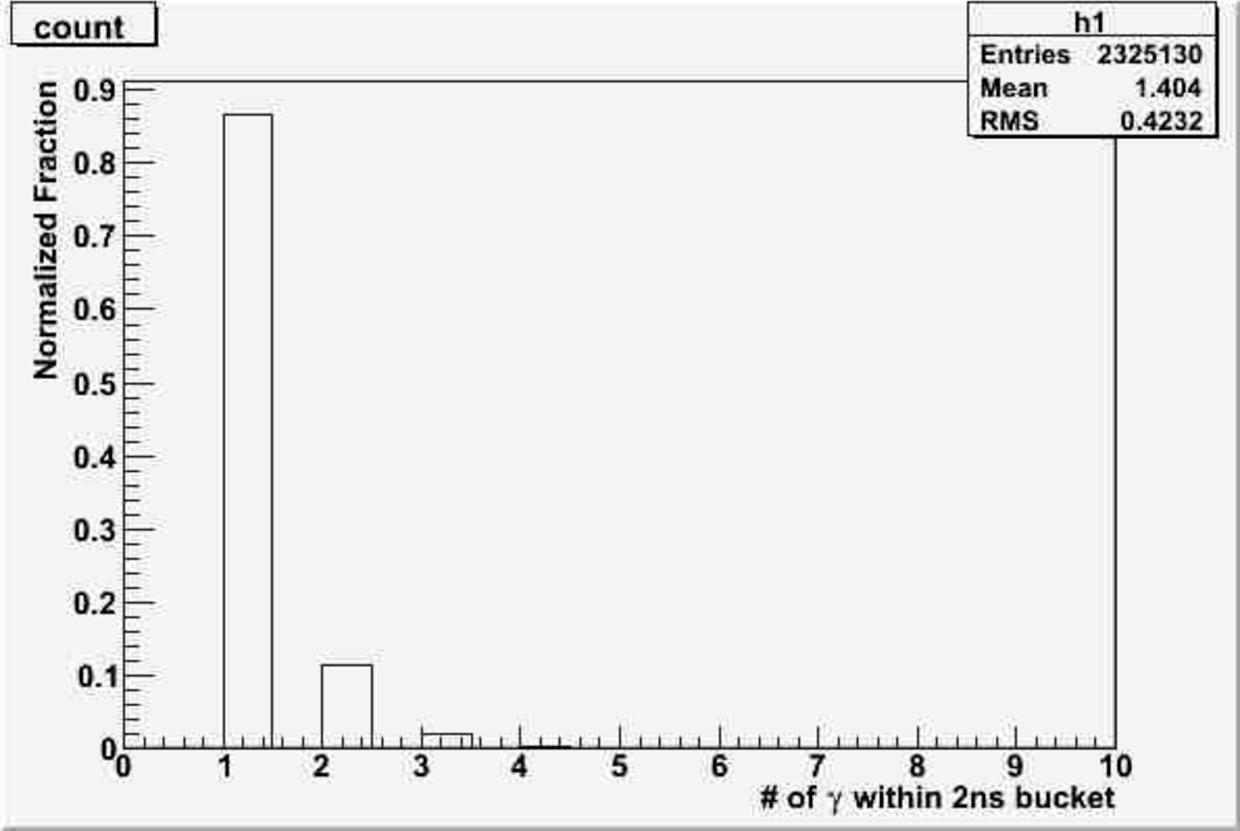
\includegraphics[width=\figwidth,height=0.75\hfigheight]{\figures/analysis/photon_timing/Photoncount1.pdf}
\caption[Probability of single and multiple photons within the \abbr{CEBAF} timing window of 2.004~ns]{\label{fig:beam.timing}Probability of single and multiple photons within the \abbr{CEBAF} timing window of 2.004~ns.}
\end{center}\end{figure}

\begin{figure}[h!]\begin{center}
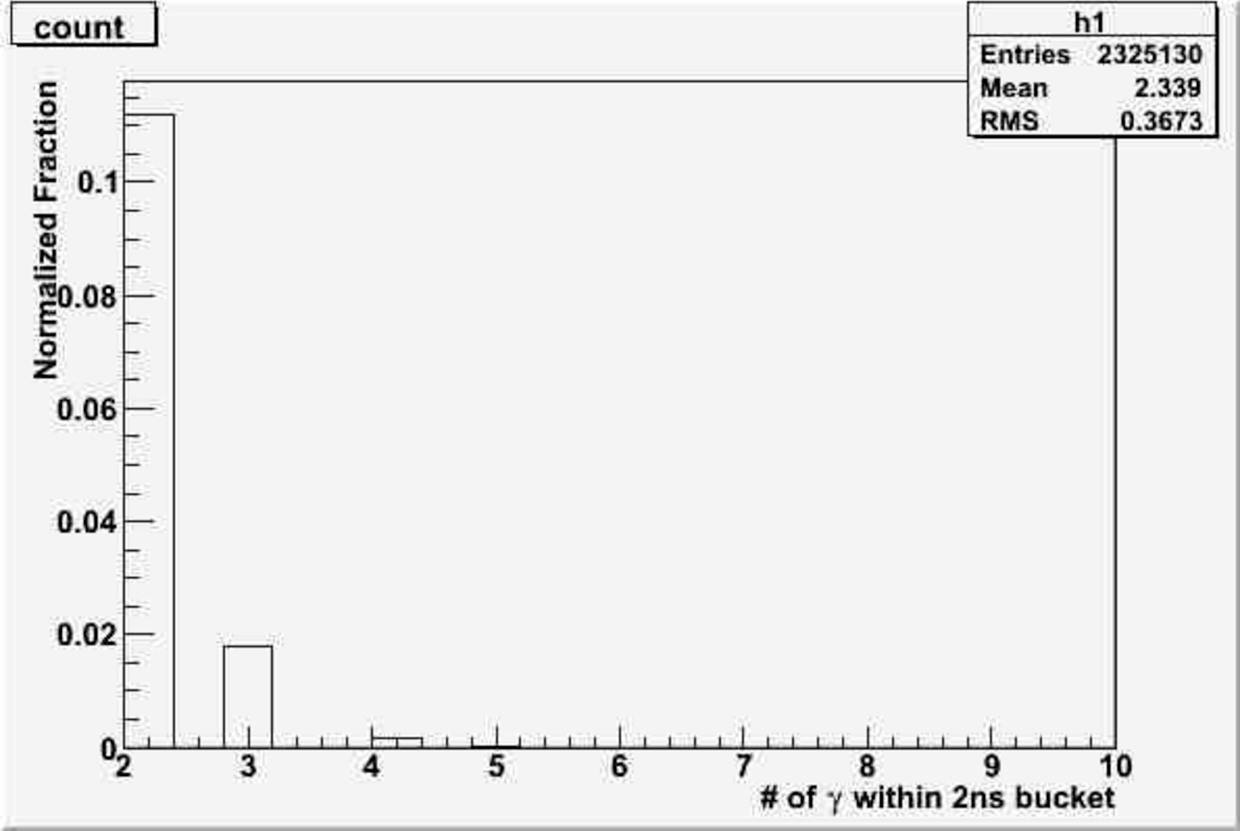
\includegraphics[width=\figwidth,height=0.75\hfigheight]{\figures/analysis/photon_timing/Photoncount.pdf}
\caption[Probability of multiple photons within the \abbr{CEBAF} timing window of 2.004~ns]{\label{fig:beam.timingII}Probability of multiple photons within the \abbr{CEBAF} timing window of 2.004~ns.}
\end{center}\end{figure}

\FloatBarrier
\subsection{Particle Identification}\label{sec:analysis.pid}

Lepton identification was based on conservation of mass. Once the data is skimmed according to Table~\ref{tab:skim.requirements}, all particles that were $\pi^+$, $\pi^-$, unknown with $q^+$ or unknown with $q^-$ were tentatively assigned to be electrons or positrons based on their charge. This meant that the mass term of the particle's 4-vector was set to be the mass of an electron instead of that of a pion. This technique works because the mass of the \piz (0.135~GeV) is less than the mass of $\pi^+$ or $\pi^-$ (0.139~GeV) and by laws of conservation of energy-momentum, a lighter particle cannot decay into heavier particle's.
%To explain this effect, lets consider a particle A decaying into daughters B and C.
%\begin{align}
%A\rightarrow B+C
%\end{align}
%In the rest frame of A the 4-momentum transforms to  
%\begin{align}
%P_A\rightarrow (0,M_A), \nonumber \\
%P_B\rightarrow (\overline{P}_B,E_B), \nonumber \\
%P_C\rightarrow (\overline{P}_C,E_C),
%\end{align}
%where $\overline{P}_B$ and $\overline{P}_C$ are the 3-momentum of particles B and C respectively. Using conservation of 4-momentum and the property $P_i^2 = m_i^2$, $E_C$ can be calculated as;
%\begin{align}\label{eq:piz.kinematics}
%P_B^2 = (P_A - P_C)^2 \nonumber \\
%M_B^2 = P_A^2 + P_C^2 - 2P_A\cdot P_C \nonumber \\
%M_B^2 = M_A^2 + M_C^2 - 2M_AE_C \nonumber \\
%E_C = \frac{M_A^2 + M_C^2 - M_B^2}{2M_A}.
%\end{align}
%For the case in which particle A is a \piz and the particles B and C are electron and positron which have equal mass eq.~\ref{eq:piz.kinematics} simplifies to 
%\begin{align}\label{eq:piz.decay}
%E_C = \frac{M_{\pi^0}^2}{2}.
%\end{align}
%The same procedure can be applied for particle B which would yield the same result as eq.~\ref{eq:piz.decay} with the interchange of the index $C\leftrightarrow B$. From eq.~\ref{eq:piz.decay} it can be seen that because 
%\begin{align}\label{eq:piz.energy}
%E_{C,B} = \sqrt{M_{C,B}^2 + \overline{P}_{C,B}^2} \nonumber
%\end{align}
%that
%\begin{align}
%M_{C,B} <  \frac{M_{\pi^0}^2}{2}, \nonumber
%\end{align}
%therefore \piz cannot decay into particles of heavier mass.

For particles with higher masses that can decay into two-pions  or into \epem, such as $\eta,\ \omega$, etc., the \abbr{CC} and \abbr{EC} provide a $\frac{e^+e^-}{\pi^+\pi^-}$ rejection factor of $\approx 10^6$. The method to achieve this rejection factor was developed by Mike Wood and is based on using various cuts placed on the \abbr{CC} and \abbr{EC} measured quantities. This method was not used in this analysis, the $\gamma p \to  p \pi^0 \to p e^+e^-\gamma$ reaction provides insight into the validity of the method. The Mike Wood method of $\frac{e^+e^-}{\pi^+\pi^-}$ rejection factor is discussed in~\cite{clas.g12.note}.   


%\section{General Features of Lepton Data in \g12}\label{sec:analysis.Lepton.general}

Electron and positron energy deposition while propagating through a material was briefly explained in Sec.~\ref{sec:clas.cc} and ~\ref{sec:clas.ec}. To identify electrons and positrons properly in \abbr{CLAS}, quantities obtained from the \abbr{CC} and \abbr{EC} are used to reject charged pions. The \abbr{CC} collects the number of photo-electrons caused by Cherenkov radiation and the \abbr{EC} records the energy deposition of electrons/positrons as well as photons. A previous \abbr{CLAS} experiment \emph{g7} analyzed the properties of medium modifications from the decay of vector mesons through the leptonic decay channel. This experiment derived a set of cits for identifying electron/positrons pairs in \abbr{CLAS} by employing specific cuts to the number of photo-electrons (\abbr{NPE}) detected in the \abbr{CC}, a match in azimuthal angle $\phi$ from a charged track in the \abbr{DC} to the $\phi$ of the \abbr{CC}, as well as comparing the momentum of the charged track to the energy deposited in the \abbr{EC}. These cuts can be found in Table~\ref{tab:ISLEP_cuts}.  
\begin{table}[h!]
\begin{minipage}{\textwidth}
\begin{center}
\begin{singlespacing}

\caption[Electron/Positron PID Cuts]{\label{tab:ISLEP_cuts}Cuts applied to the \abbr{CC} and \abbr{EC} to perform electron/positron \abbr{PID} \vspace{0.75mm}}

\begin{tabular}{c|c|c}

\hline
Subsystem & Quantity & Cut \\
\hline
\multirow{2}{*}{\abbr{CC}}  & \# of photo-electrons (\abbr{NPE})  & \abbr{NPE} $>$ 2.5 \\
 &  \abbr{DC} $\phi$ \& \abbr{CC} $\phi$  & \abbr{DC} $\phi$ = \abbr{CC} $\phi$ \\
\hline
\multirow{2}{*}{\abbr{EC}}  & q$^{\pm}$ momentum threshold (p$\mathrm{_{thres}}$) & \multirow{2}{*}{p$\mathrm{_{thres}^{high}} < \ $E$\mathrm{_{calo}} <$ p$\mathrm{_{thres}^{low}}$ } \\
&  \& \abbr{EC} deposited energy (E$\mathrm{_{calo}}$) & \\
\hline \hline
\end{tabular}

%\begin{tabular}{c|c|c}
%\hline
%Subsystem & Quantity & Cut   \vspace{0.5mm} \\
%\hline
%\multirow{2}{*}{\abbr{CC}}  & \# of photo-electrons (\abbr{NPE})  & \abbr{NPE} $>$ 2.5 \\
% &  \abbr{DC} $\phi$ \& \abbr{CC} $\phi$  & \abbr{DC} $\phi$ = \abbr{CC} $\phi$ \\
%\hline
% \multirow{2}{*}{\abbr{EC}}  & q$^{\pm}$ momentum threshold (p$\mathrm{_{thres}}$) \& \abbr{EC} deposited energy (E$\mathrm{_{calo}}$)& p$\mathrm{_{thres}^{low}}$ $<$E$\mathrm{_{calo}}$ \\
%  &  q$^{\pm}$ momentum \& \abbr{EC} deposited energy  & \abbr{DC} $\phi$ = \abbr{CC} $\phi$ \\
%\hline \hline
%\end{tabular}  


\end{singlespacing}
\end{center}
\end{minipage}
\end{table}
\vspace{20pt}
To validate the \emph{g7} electron/positron \abbr{PID} scheme for \g12, a comparison of  the \abbr{CC} and \abbr{EC} quantities was performed for all charged tracks \abbr{CC}/\abbr{EC} hit signatures and while selecting events from \piz decay. To separate the \piz events from the $\pi^{+}\pi^{-}$ events, all charged pions were assigned the mass of electrons and cuts were placed on the missing energy of $\gamma p \rightarrow p e^+ e^-$ as well as a cut on the missing mass squared of $\gamma p \rightarrow p$, values found in Table~\ref{tab:lep_cuts}. A graphical depiction of the cuts applied to separate \piz events from the $\pi^{+}\pi^{-}$ events is seen in Fig.~\ref{fig:islep.cuts}.
\begin{table}[h!]
\begin{minipage}{\textwidth}
\begin{center}
\begin{singlespacing}

\caption[Cuts To Seperate \piz from $\pi^{+}\pi^{-}$ for \abbr{PID} Validation]{\label{tab:lep_cuts}Cuts applied to seperate \piz evetns from $\pi^{+}\pi^{-}$ events \vspace{0.75mm}}

\begin{tabular}{c|c|c}

\hline
Cut Topology & Topology Quantity & Value  \\
\hline
$\gamma p \rightarrow p e^+ e^-$ & Missing Energy ($\mathrm{M_E}$) & $>0.075$~GeV \\
\hline
\multirow{2}{*}{$\gamma p \rightarrow p $}  & \multirow{2}{*}{Missing mass squared ($\mathrm{M_x^2}$)} & $<$ 0.0779~GeV$^2$ for \piz events \\
&  & $>$ 0.0779~GeV$^2$ for $\pi^{+}\pi^{-}$ events\\
\hline \hline
\end{tabular}

\end{singlespacing}
\end{center}
\end{minipage}
\end{table}
\vspace{20pt} 
The values of the threshold momentum are calculated from empirical studies and are based upon calculations using the momentum obtained from the \abbr{DC }$p$ under the following criteria;
\begin{align}
\mathrm{p_{thres}^{low}} = \alpha p *(p+EC_{P\_LO})/p \nonumber \\
\mathrm{p_{thres}^{high}} = \alpha p *(p+EC_{P\_HIGH})/p \nonumber
\end{align}
where $EC_{P\_LO} = -0.3$, $EC_{P\_HIGH} = 0.5$ and  
\begin{align}
\alpha p =
\begin{cases}
.23*p + .071p^2 - .032p^3, & p<1.0 \mathrm{~GeV} \\
0.272p, & p>1.0 \mathrm{~GeV} \\
\end{cases}\nonumber
\end{align}


\begin{figure}[h!]\begin{center}
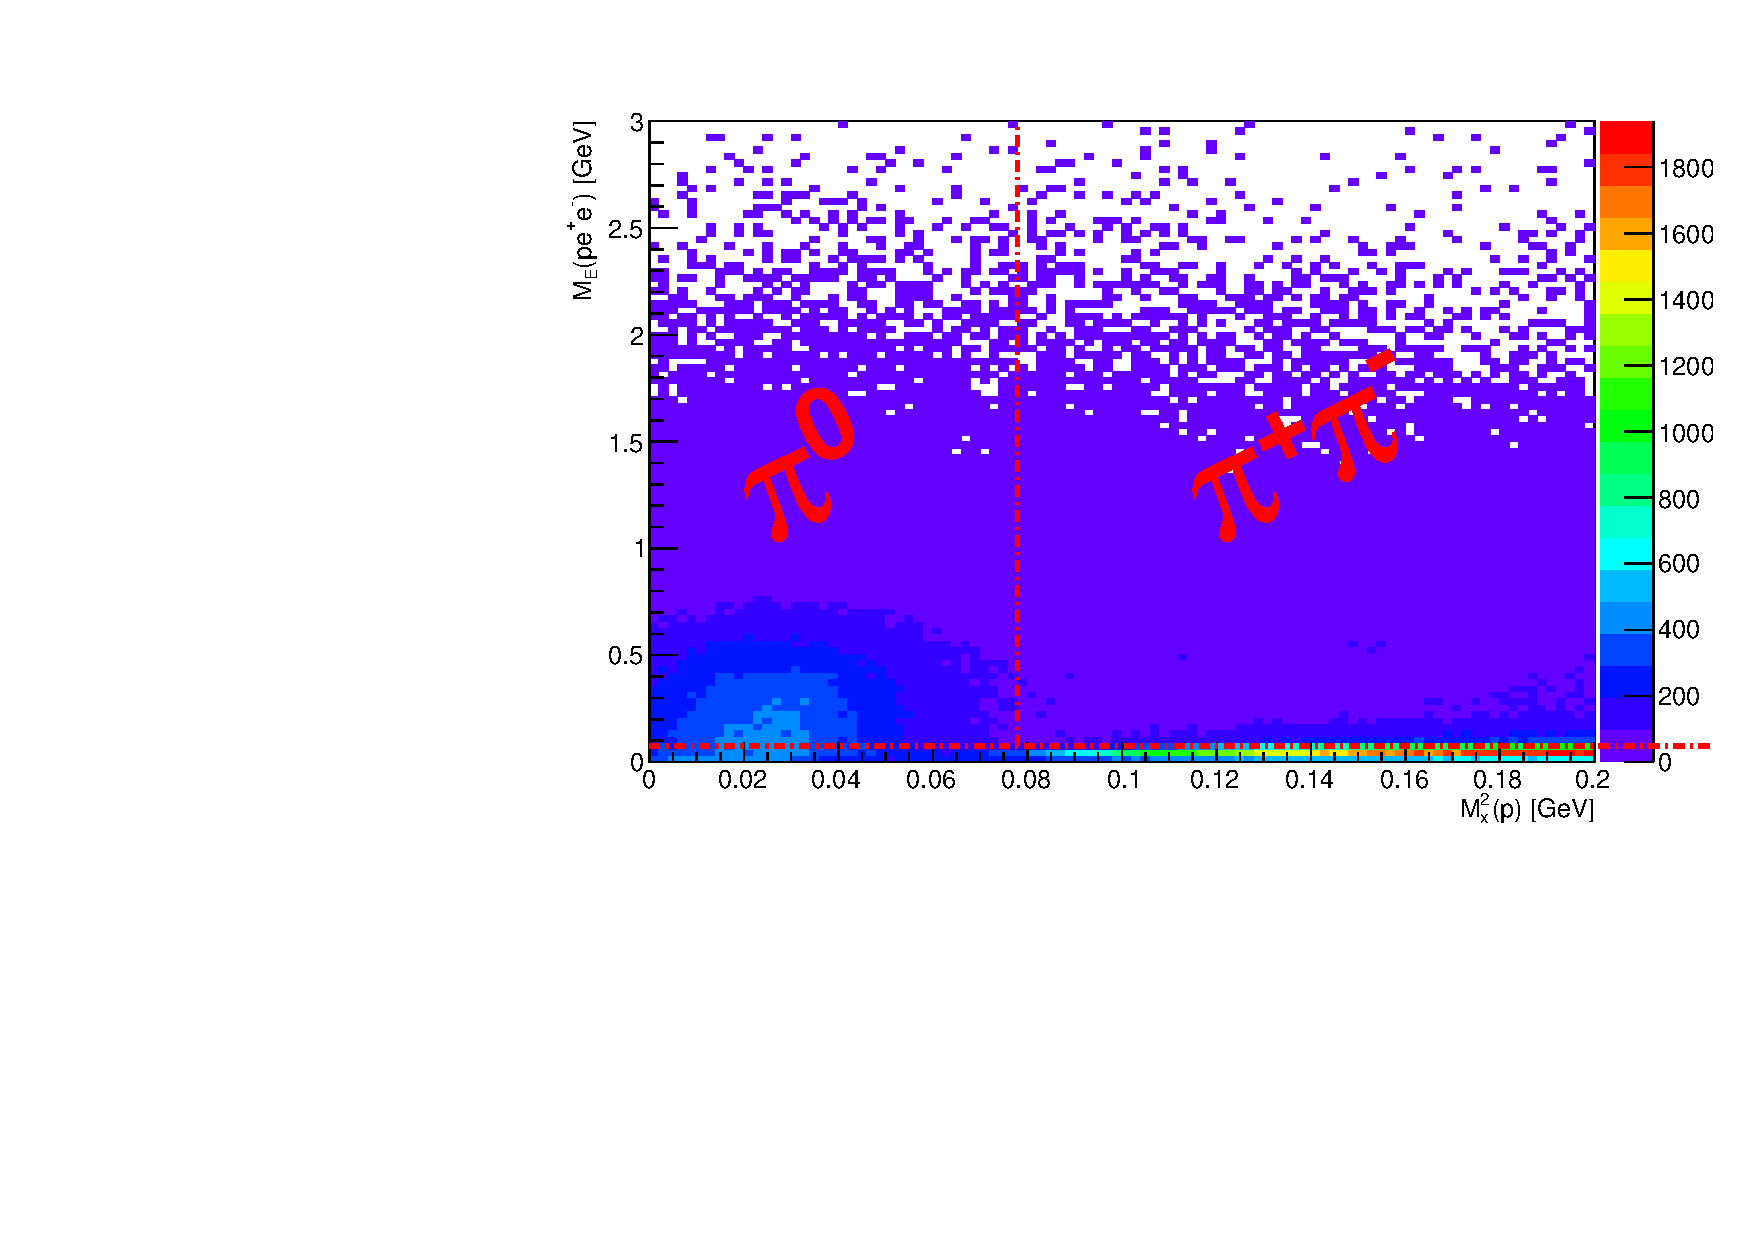
\includegraphics[width=\figwidth,height=\hfigheight]{\figures/analysis/LEP_FEATURES/Lepfeature_cuts.pdf}
\caption[Cuts Applied to Isolate \piz and $\pi^{+}\pi^{-}$ for \abbr{PID} Validation]{\label{fig:islep.cuts}Plot of missing mass squared of off proton (horizontal) vs. missing energy of proton e$^+$e$^-$ (vertical). The red dashed vertical line depicts the $\pi^{+}\pi^{-}$ threshold mass cut while the horizontal red dashed line represents the missing energy cut-off used to sepertate $\pi^{+}\pi^{-}$ from \piz.}
\end{center}\end{figure}

\subsubsection{\abbr{CC} Comparison}

The \abbr{NPE} measured by the \abbr{CC} for all positron/electron (e$^+$/e$^-$) candidates can be seen in Fig~\ref{fig:islep.CC}. The sharp decline prior to 2.5 \abbr{NPE} is due to photo-electrons created by electron/positrons, pions traveling through the \abbr{CC} or pions producing delta-electrons which pass through the \abbr{CC}. Delta-electrons are created as an effect of the ionization of gases that could be present when the pion travels through the \abbr{DC}. These types of electrons are typically lower in momentum than the electrons obtained from particle decays in \abbr{CLAS} and thus according to eq.~\ref{eq:cc.NPE} should emit less \abbr{NPE} per unit length.

Through mass conservation, as discussed in Sec.~\ref{sec:analysis.pid}, the particles in the \piz events must be e$^+$/e$^-$ pairs. In comparison to fig.~\ref{fig:islep.CC}, fig.~\ref{fig:islep.CC1} plots the \abbr{NPE} measured by the \abbr{CC} for all e$^+$/e$^-$ pairs for \piz events selected as shown in fig.~\ref{fig:islep.cuts}. It can be seen that the sharp decline prior to \abbr{NPE} = 2.5 is reduced leaving mostly electrons or positrons signatures in the \abbr{CC} concluding that the \emph{g7} \abbr{CC} \abbr{NPE} cut is valid for identifying e$^+$/e$^-$ pairs while rejecting $\pi^+$/$\pi^-$ pairs.
 
%
\begin{figure}[h!]\begin{center}
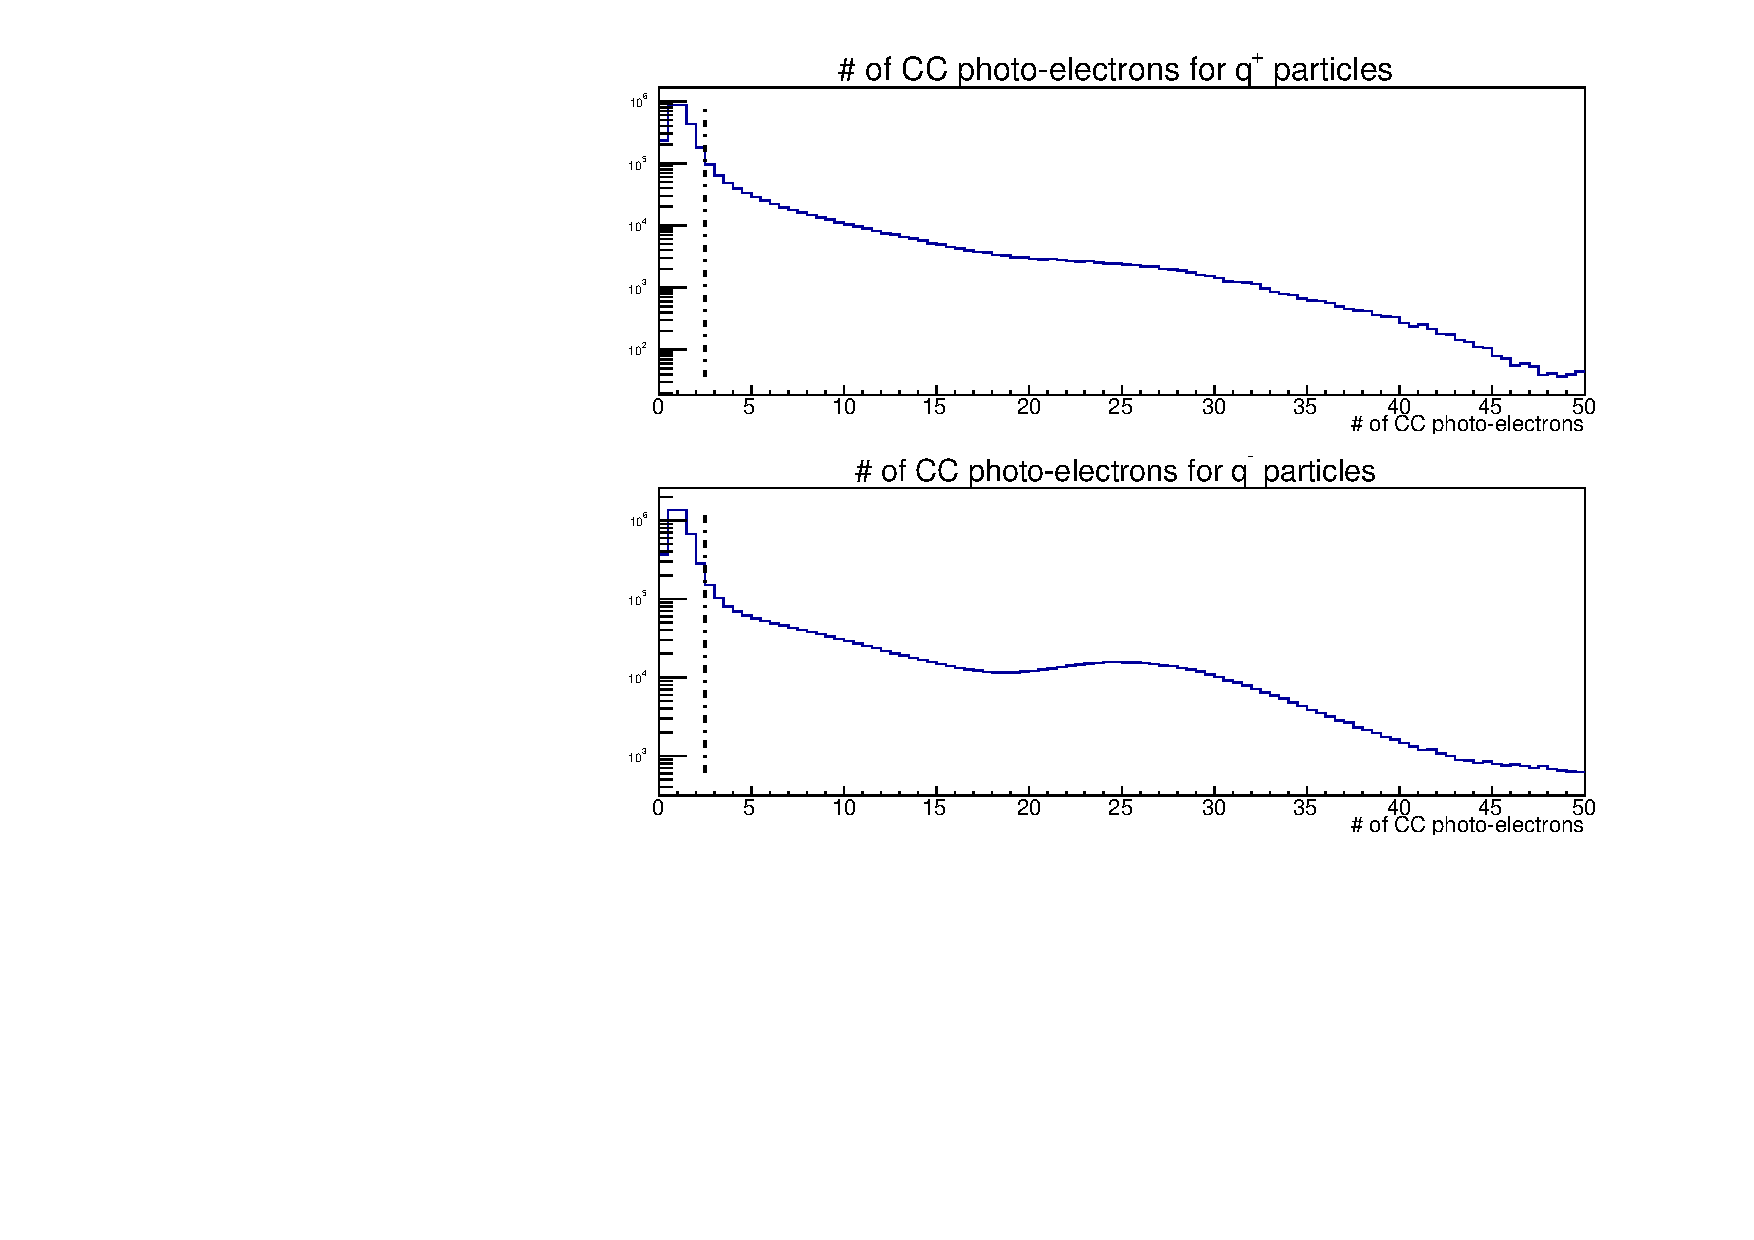
\includegraphics[width=\figwidth,height=\hfigheight]{\figures/analysis/LEP_FEATURES/CC_nPE.pdf}
\caption[Number of Photo-electrons Measured by \abbr{CC} for All e$^-$ and e$^+$ Candidates]{\label{fig:islep.CC}Plot of \abbr{NPE} measured by \abbr{CLAS} \abbr{CC} subsystem for positron/electron candidates top/bottom respectively. The dashed dotted vertical line depicts the cut applied if using the \emph{g7} lepton \abbr{PID} scheme.}
\end{center}\end{figure}

\begin{figure}[h!]\begin{center}
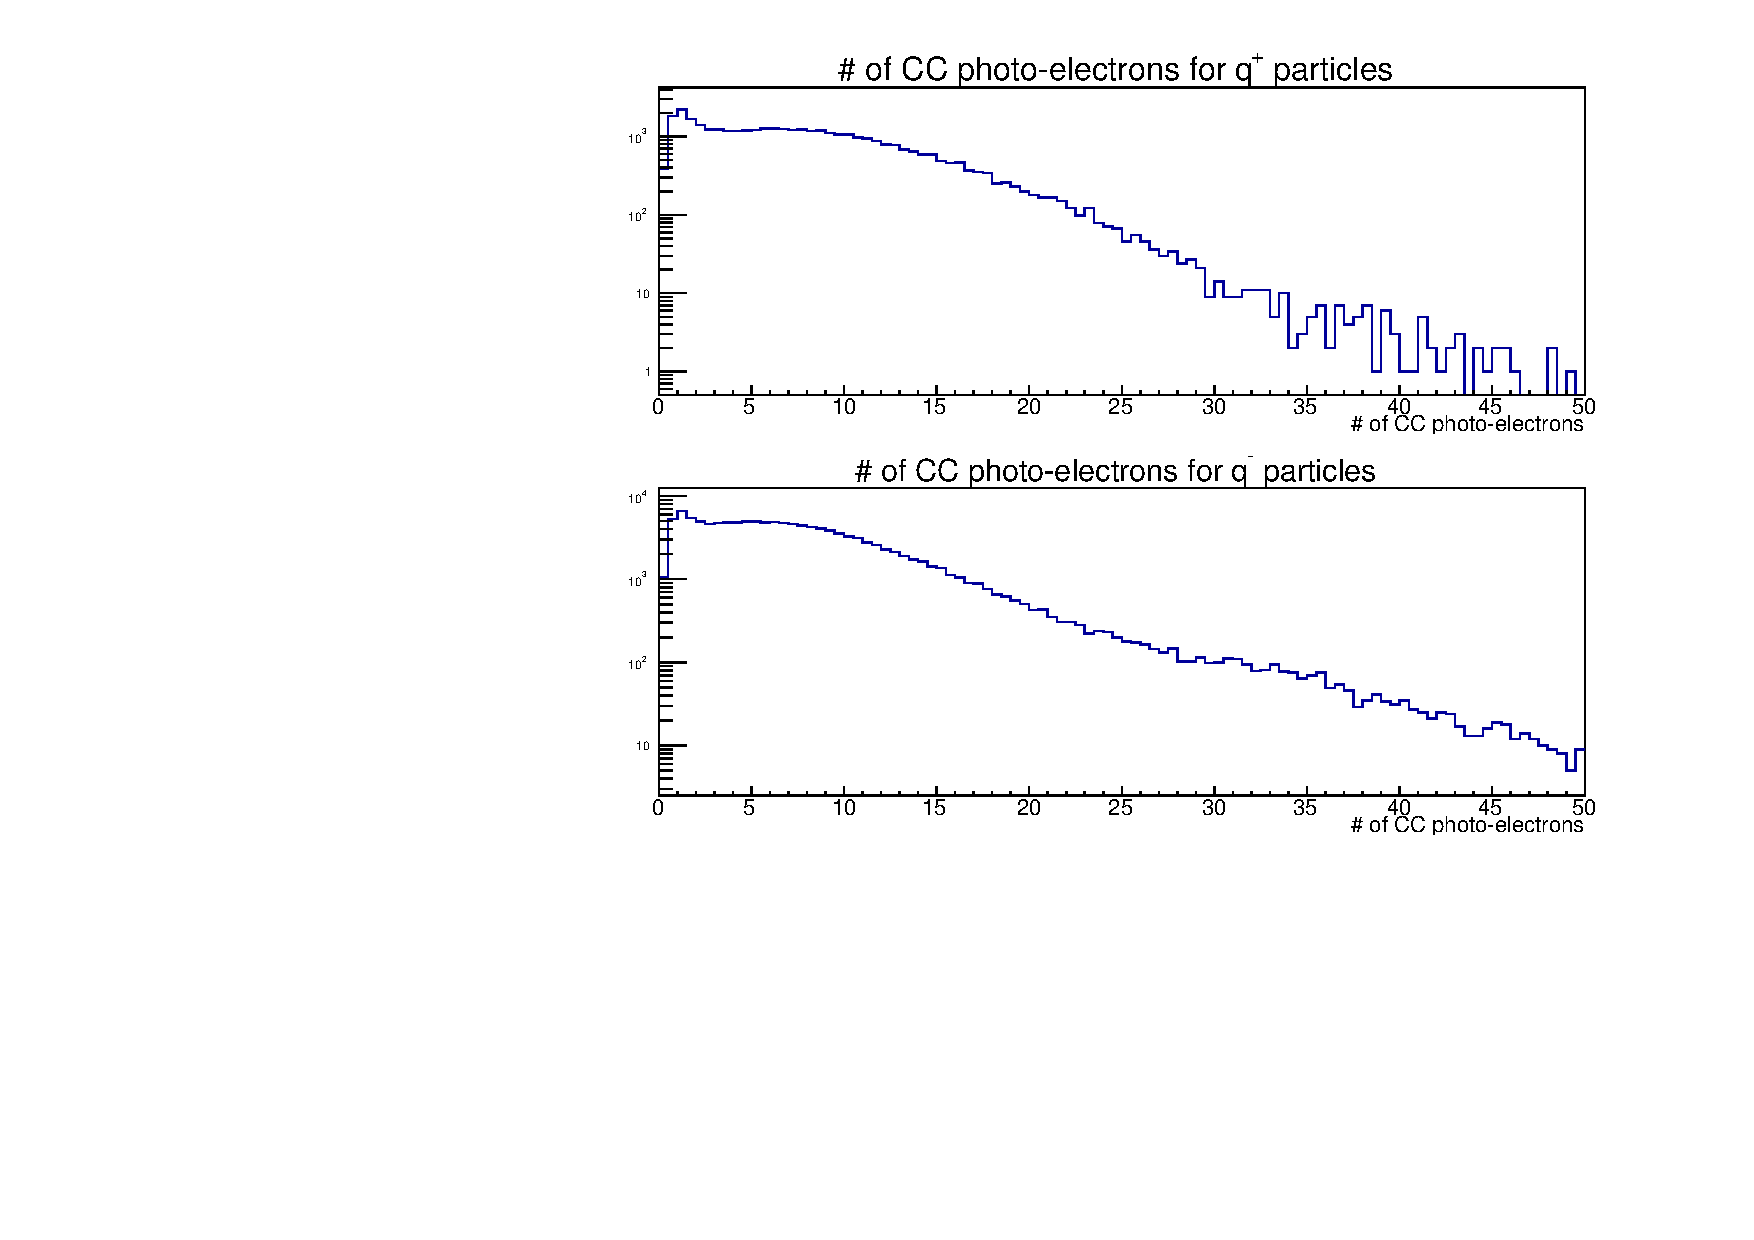
\includegraphics[width=\figwidth,height=\hfigheight]{\figures/analysis/LEP_FEATURES/CC_NPEcut.pdf}
\caption[Number of Photo-electrons Measured by \abbr{CC} for \piz Events]{\label{fig:islep.CC1}Plot of \abbr{NPE} measured by \abbr{CLAS} \abbr{CC} subsystem when selecting \piz events seen in Fig~\ref{fig:islep.cuts}, positron/electron candidates top/bottom respectively.}
\end{center}\end{figure}
\FloatBarrier
\subsubsection{\abbr{EC} Comparison}
%EC
%
%e-
%

Similarly to the \abbr{CC} comparison, figures~\ref{fig:islep.pimEClow},~\ref{fig:islep.pimEChigh},~\ref{fig:islep.pipEClow},~\ref{fig:islep.pipEChigh} depict the  p$\mathrm{_{thres}^{low}}$ and  p$\mathrm{_{thres}^{low}}$ cuts listed in  Table~\ref{tab:ISLEP_cuts} for the q$^-$ and q$^+$ tracks respectively. After \piz event selection, seen in figures~\ref{fig:islep.pimEC},~\ref{fig:islep.pimECcut} ,~\ref{fig:islep.pipEC} ,~\ref{fig:islep.pipECcut}, the bulk of e$^+$/e$^-$ events reside within the region of the cut acceptance therefore it is evident that the \emph{g7} \abbr{EC} cuts are valid for identifying e$^+$/e$^-$ pairs. The following four plots are for electron($e^-$) \abbr{PID} validation of the \emph{g7} \abbr{EC} cuts described in Table~\ref{tab:ISLEP_cuts}.
%
\begin{figure}[h!]\begin{center}
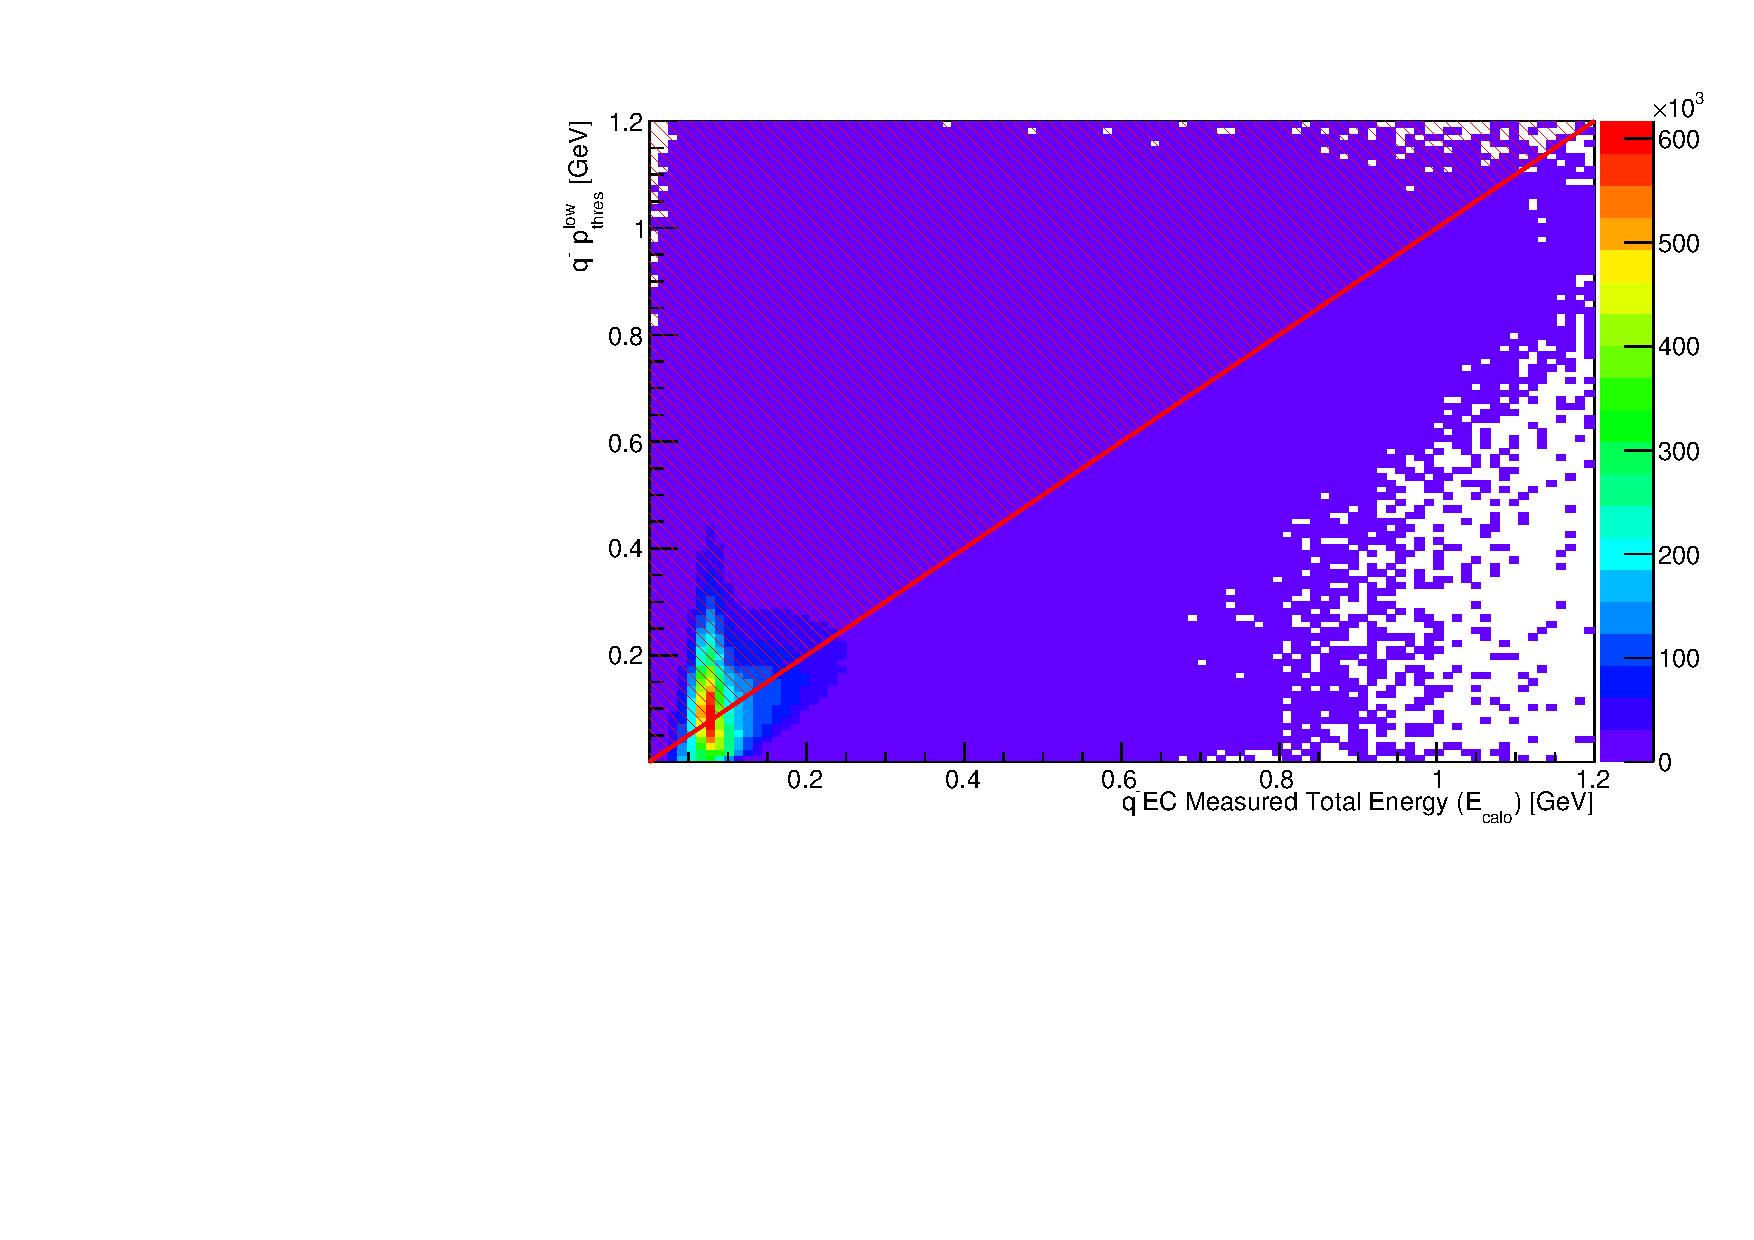
\includegraphics[width=\figwidth,height=0.7\hfigheight]{\figures/analysis/LEP_FEATURES/Pim_EClow.pdf}
\caption[\abbr{EC} Deposited Energy Comparison to Lower Threshold Track Momentum for q$^-$ Tracks]{\label{fig:islep.pimEClow}Plot of energy deposited measured by \abbr{EC} vs. track momentum p$\mathrm{_{thres}^{low}}$ for negative charged tracks. The red region depicts the cut that would reject events in the \emph{g7} lepton \abbr{EC} \abbr{PID} scheme.}
\end{center}\end{figure}

\begin{figure}[h!]\begin{center}
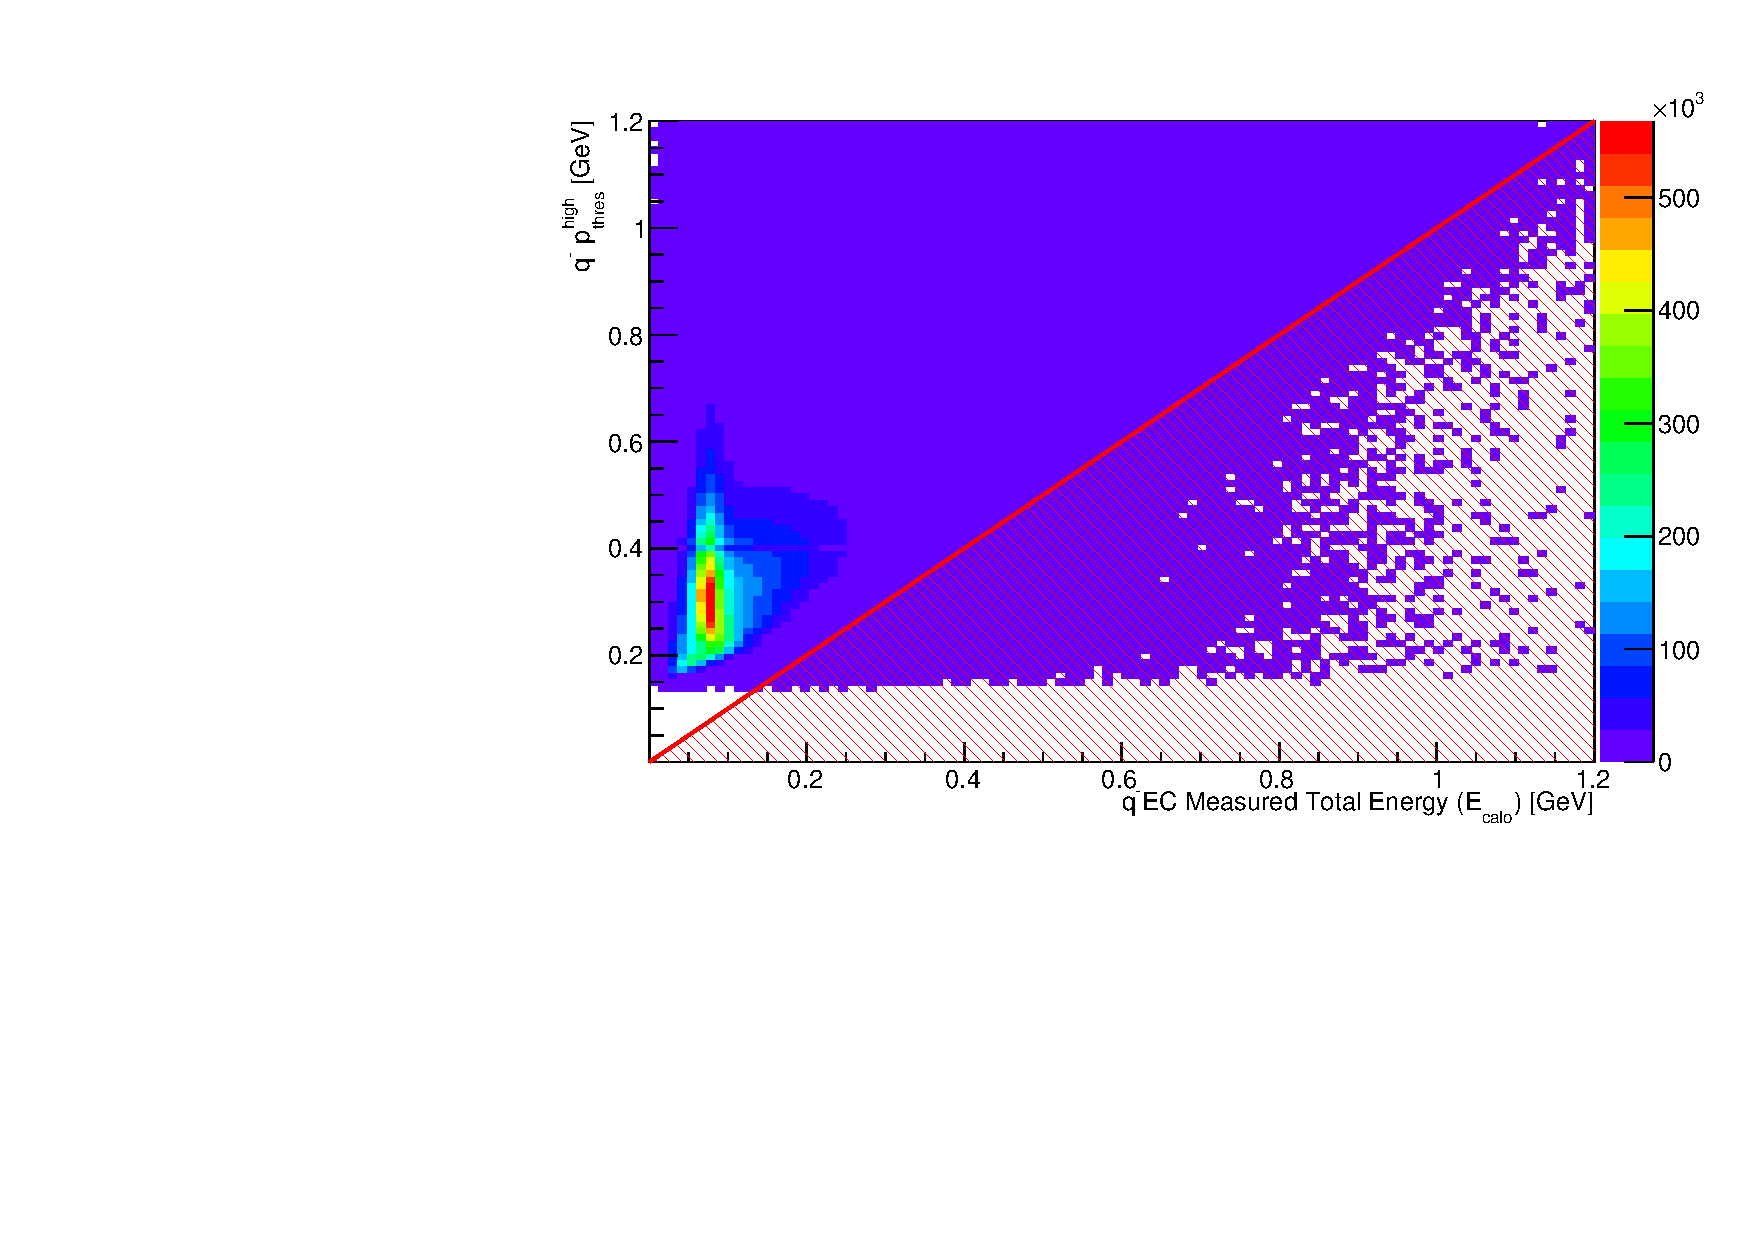
\includegraphics[width=\figwidth,height=0.7\hfigheight]{\figures/analysis/LEP_FEATURES/Pim_EChigh.pdf}
\caption[\abbr{EC} Deposited Energy Comparison to Upper Threshold Track Momentum for q$^-$ Tracks]{\label{fig:islep.pimEChigh}Plot of energy deposited measured by \abbr{EC} vs. track momentum p$\mathrm{_{thres}^{high}}$ for negative charged tracks. The red region depicts the cut that would reject events in the \emph{g7} lepton \abbr{EC} \abbr{PID} scheme.}
\end{center}\end{figure}


\begin{figure}[h!]\begin{center}
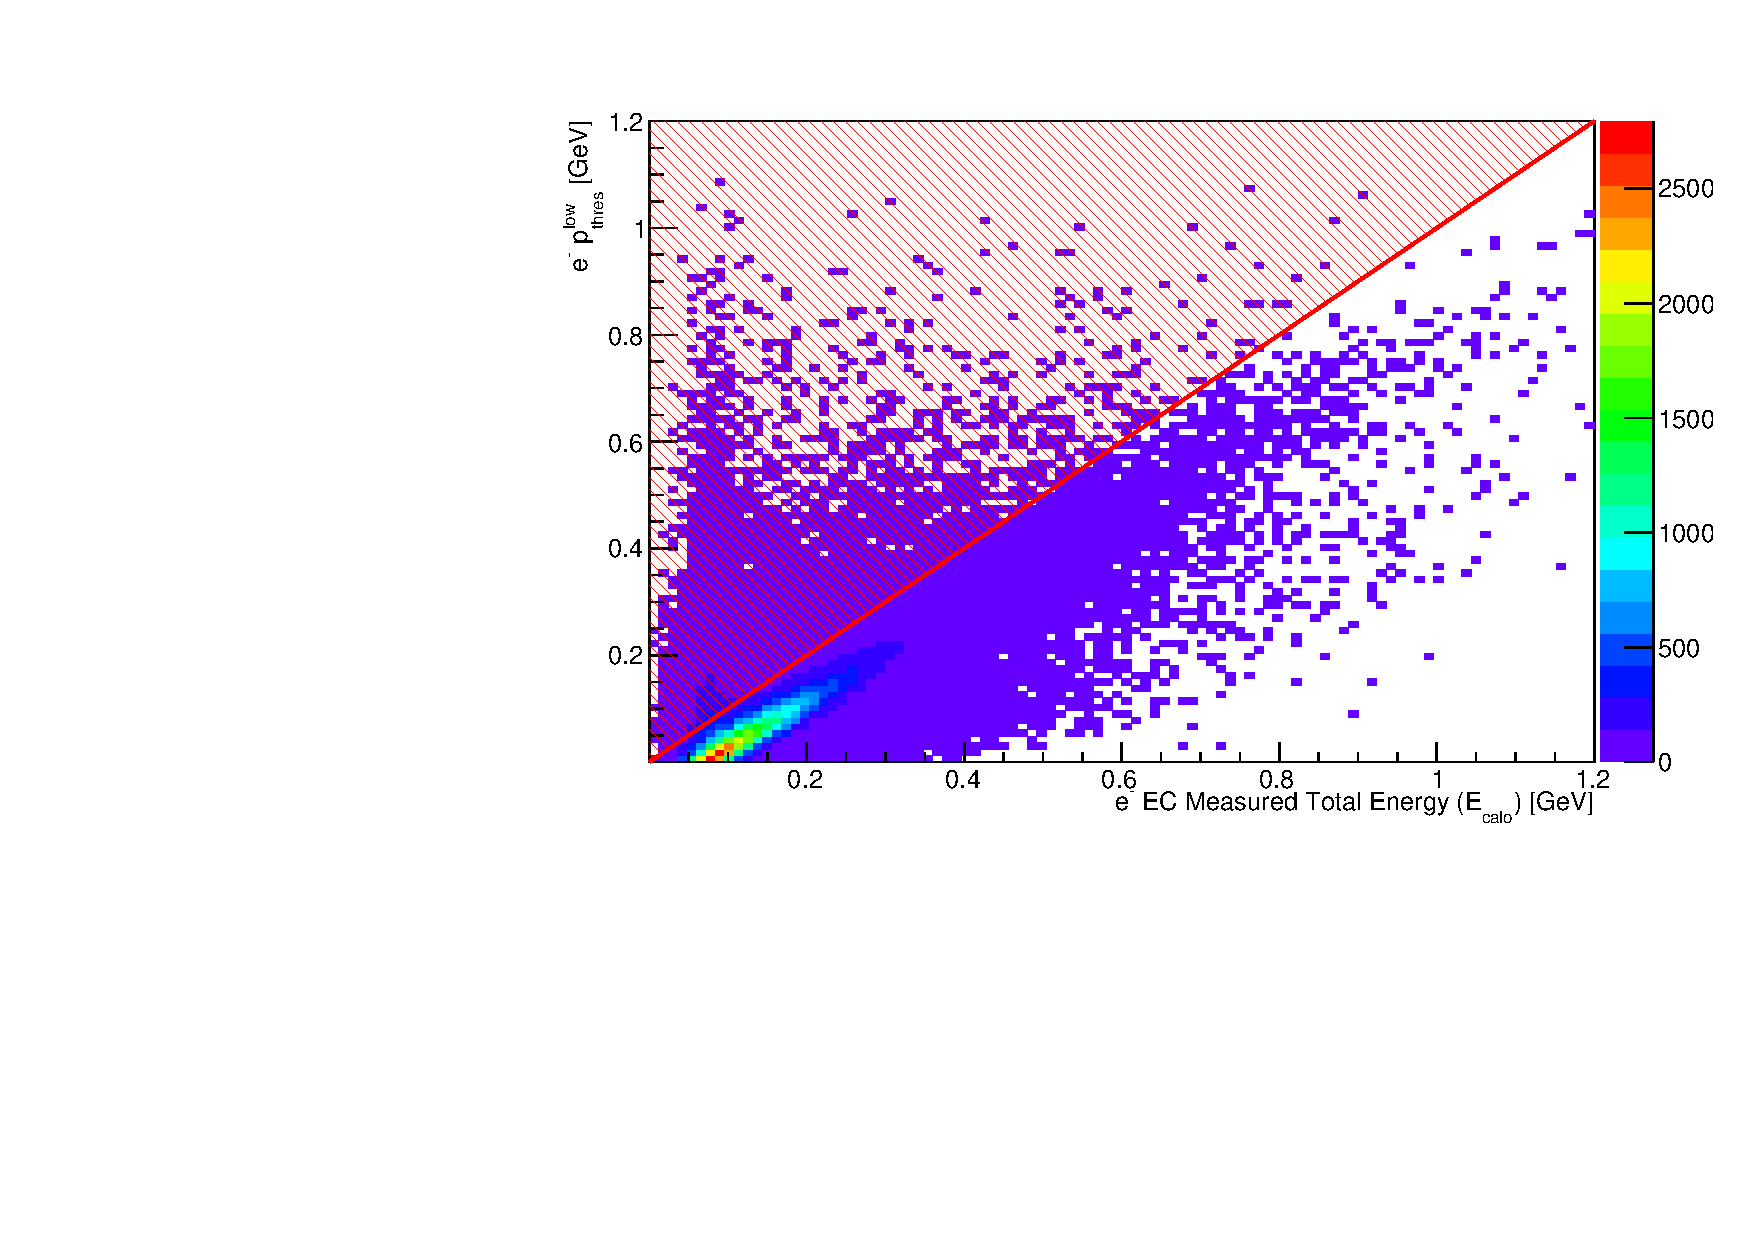
\includegraphics[width=\figwidth,height=0.7\hfigheight]{\figures/analysis/LEP_FEATURES/Pim_EClowcut.pdf}
\caption[\abbr{EC} Deposited Energy Comparison to Track Momentum for e$^-$ Candidates]{\label{fig:islep.pimEC}Plot of energy deposited measured by \abbr{EC} vs. track momentum p$\mathrm{_{thres}^{low}}$ for electrons from \piz events without the \emph{g7} lepton \abbr{EC} \abbr{PID} scheme applied. The red region depicts the cut that would reject events in the \emph{g7} lepton \abbr{EC} \abbr{PID} scheme.}
\end{center}\end{figure}

\begin{figure}[h!]\begin{center}
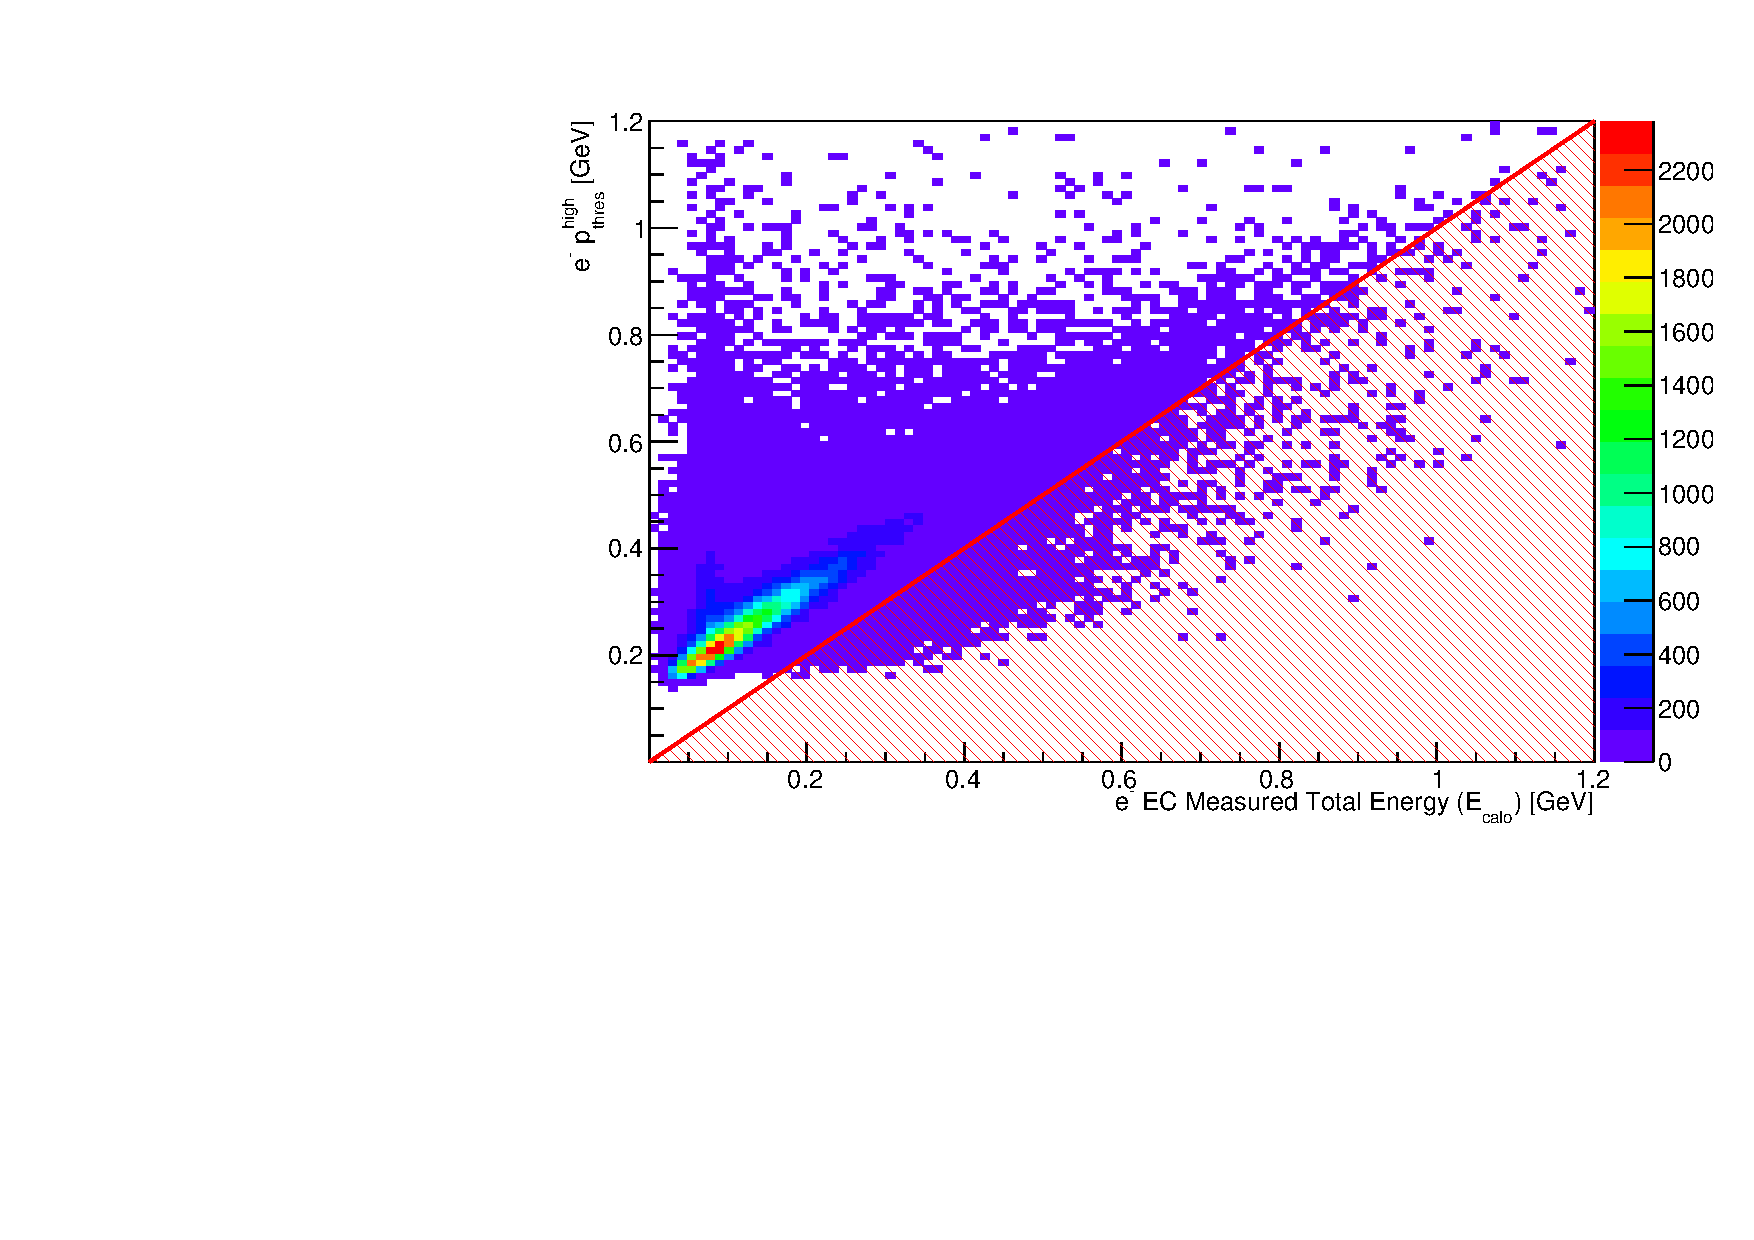
\includegraphics[width=\figwidth,height=0.7\hfigheight]{\figures/analysis/LEP_FEATURES/Pim_EChighcut.pdf}
\caption[\abbr{EC} Deposited Energy Comparison to Track Momentum for e$^-$ from \piz Events]{\label{fig:islep.pimECcut}Plot of energy deposited measured by \abbr{EC} vs. track momentum p$\mathrm{_{thres}^{high}}$ for electrons from \piz events without the \emph{g7} lepton \abbr{EC} \abbr{PID} scheme applied. The red region depicts the cut that would reject events in the \emph{g7} lepton \abbr{EC} \abbr{PID} scheme.}
\end{center}\end{figure}
\FloatBarrier
The following four plots are for positron($e^+$) \abbr{PID} validation of the \emph{g7} \abbr{EC}
cuts described in Table~\ref{tab:ISLEP_cuts}.
%
%
%e+
%
%
\begin{figure}[h!]\begin{center}
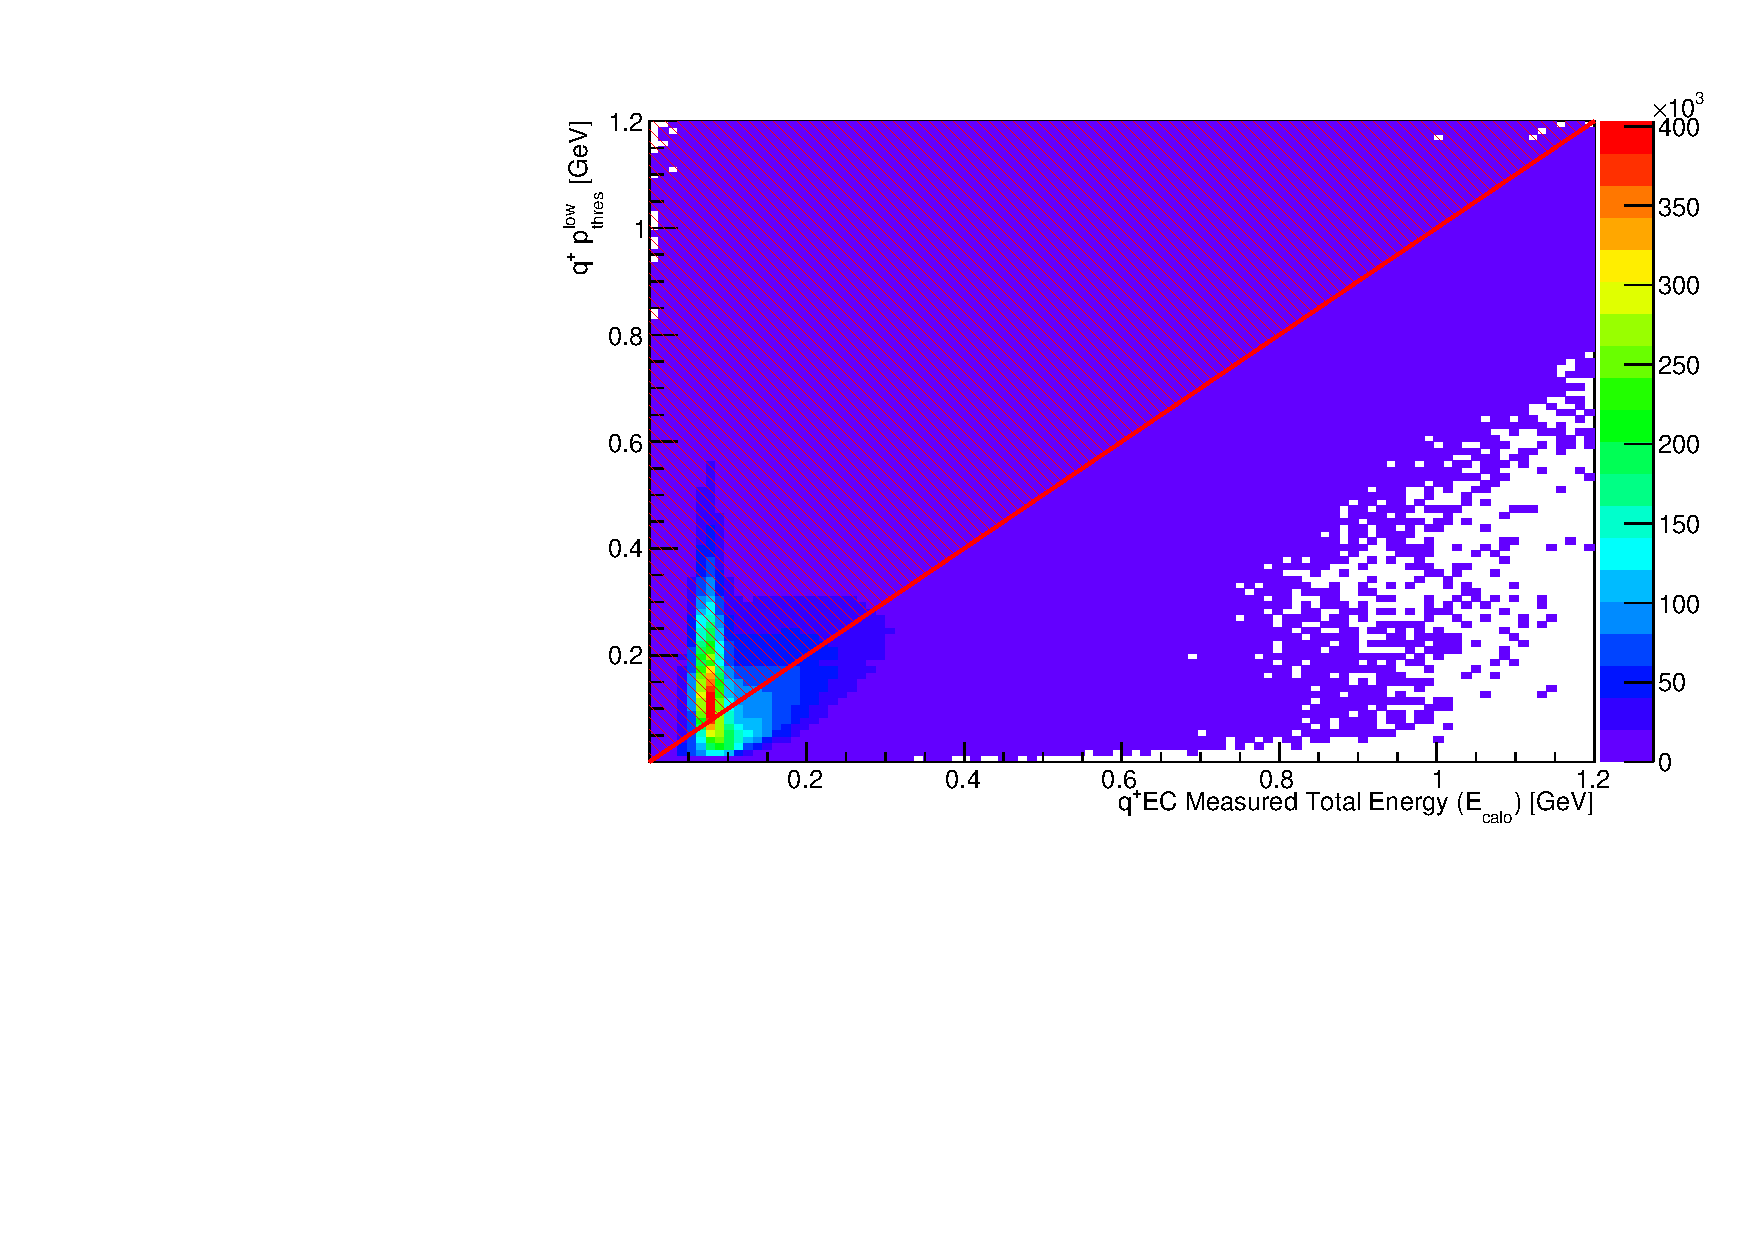
\includegraphics[width=\figwidth,height=0.7\hfigheight]{\figures/analysis/LEP_FEATURES/Pip_EClow.pdf}
\caption[\abbr{EC} Deposited Energy Comparison to Lower Threshold Track Momentum for q$^+$ Tracks]{\label{fig:islep.pipEClow}Plot of energy deposited measured by \abbr{EC} vs. track momentum p$\mathrm{_{thres}^{low}}$ for positive charged tracks. The red region depicts the cut that would reject events in the \emph{g7} lepton \abbr{EC} \abbr{PID} scheme.}
\end{center}\end{figure}

\begin{figure}[h!]\begin{center}
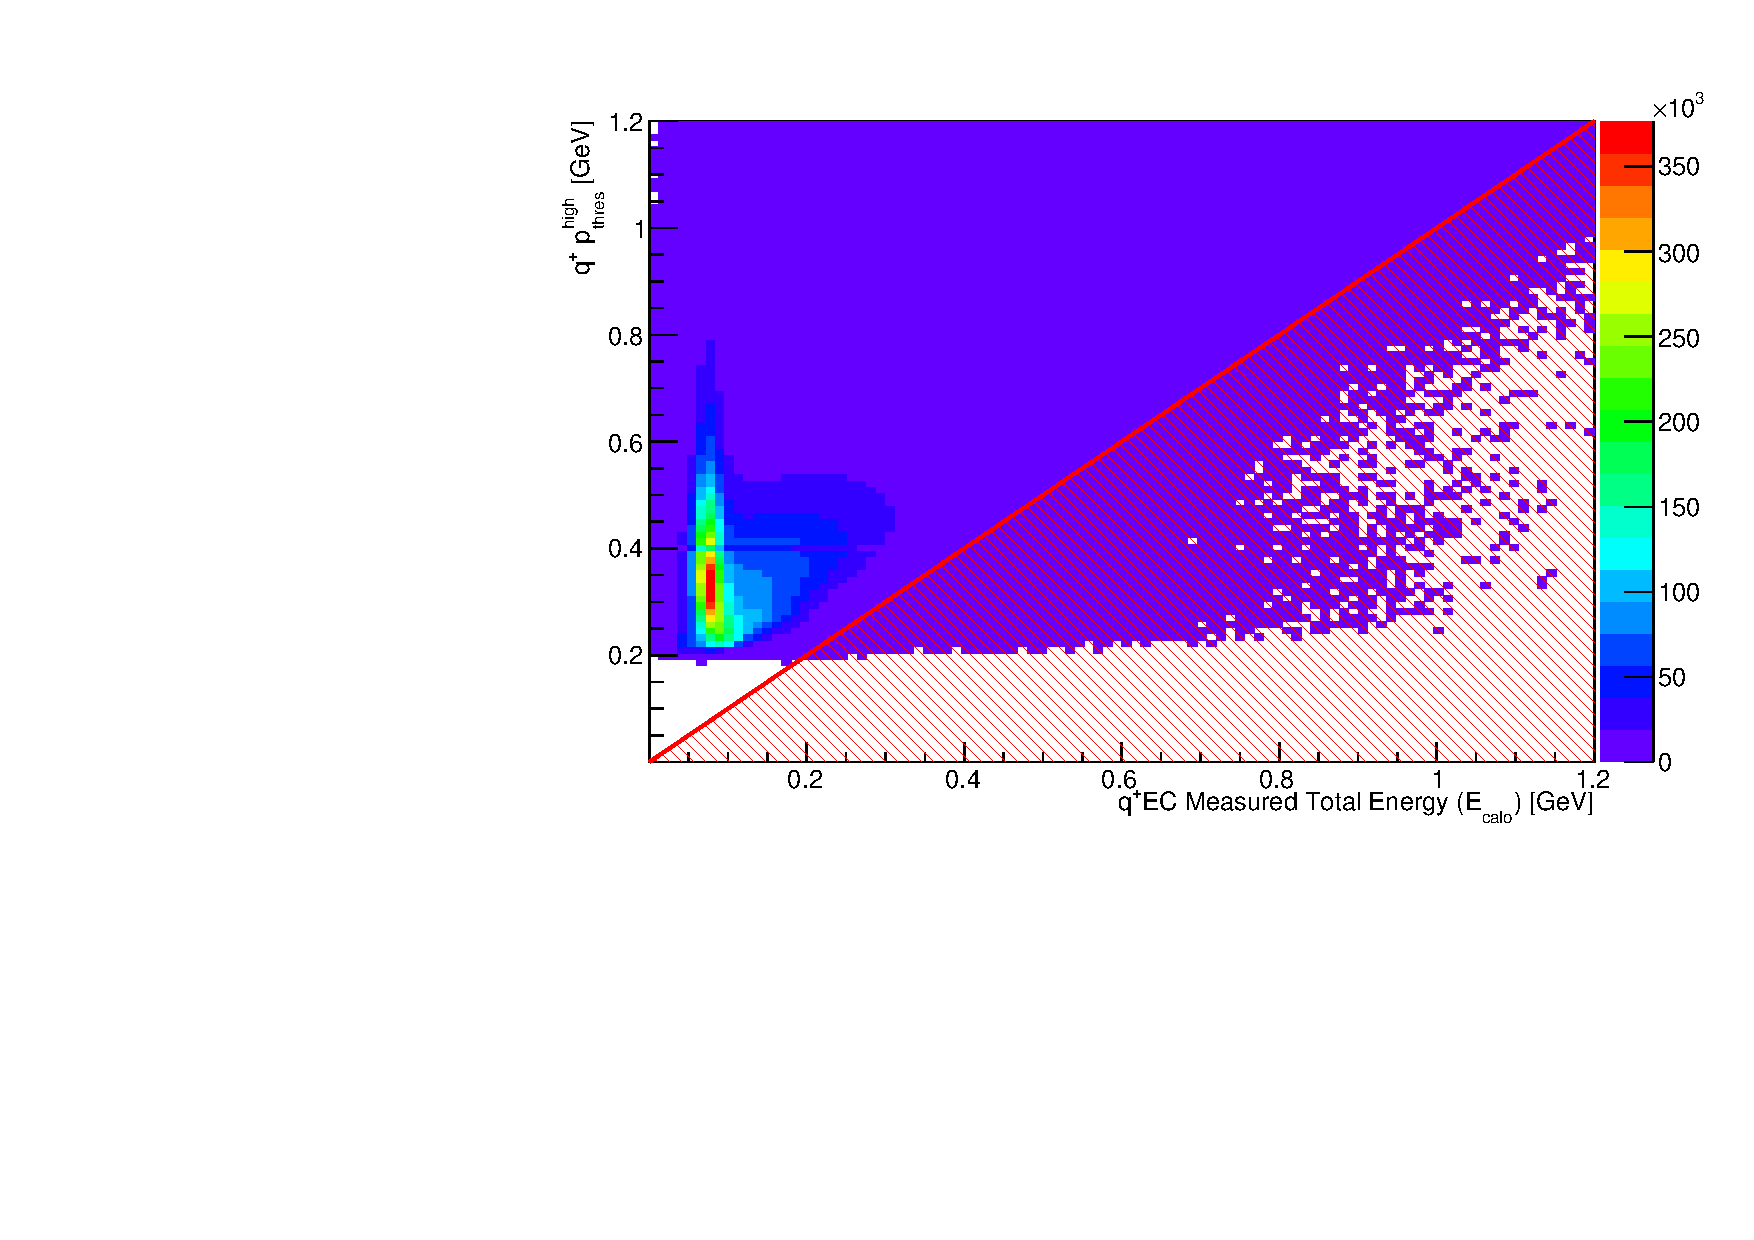
\includegraphics[width=\figwidth,height=0.7\hfigheight]{\figures/analysis/LEP_FEATURES/Pip_EChigh.pdf}
\caption[\abbr{EC} Deposited Energy Comparison to Upper Threshold Track Momentum for q$^+$ Tracks]{\label{fig:islep.pipEChigh}Plot of energy deposited measured by \abbr{EC} vs. track momentum p$\mathrm{_{thres}^{high}}$ for positive charged tracks. The red region depicts the cut that would reject events in the \emph{g7} lepton \abbr{EC} \abbr{PID} scheme.}
\end{center}\end{figure}

\begin{figure}[h!]\begin{center}
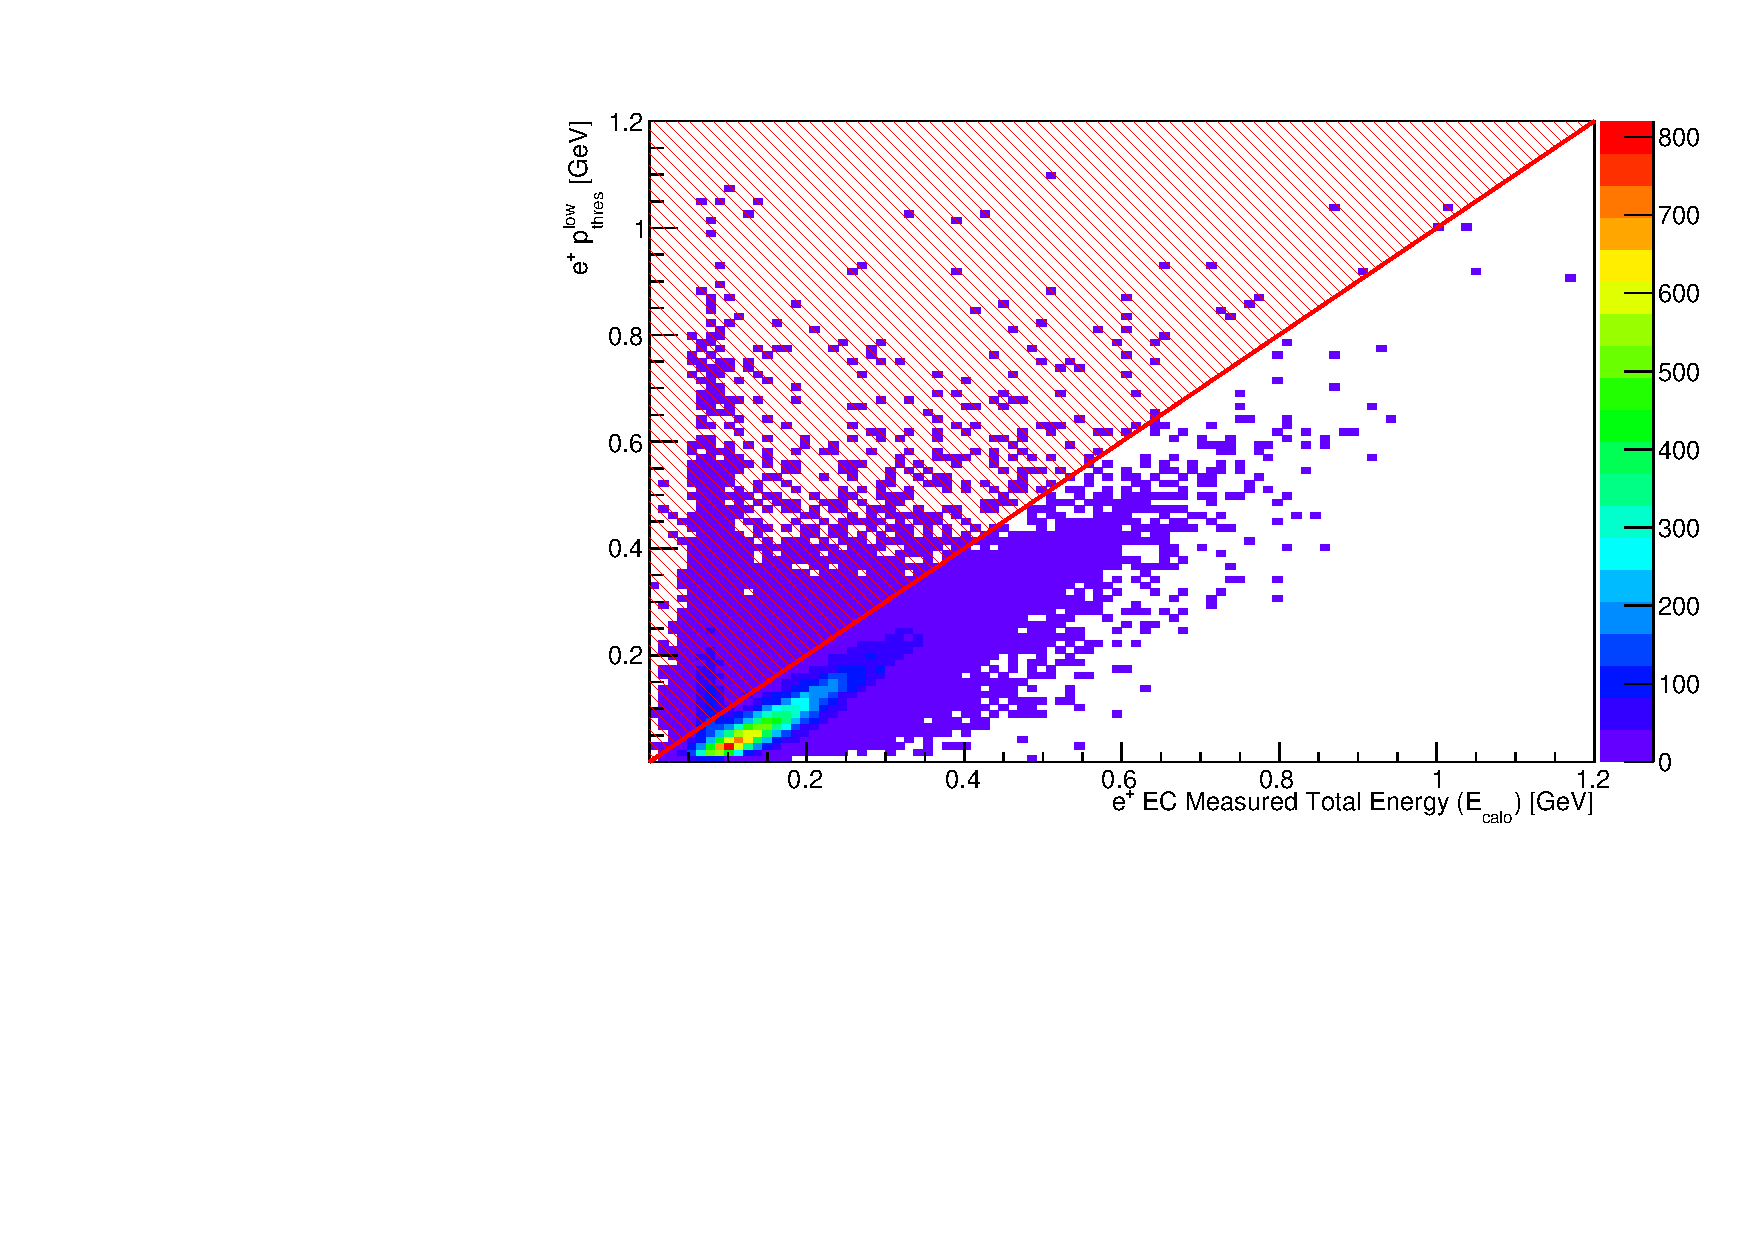
\includegraphics[width=\figwidth,height=0.7\hfigheight]{\figures/analysis/LEP_FEATURES/Pip_EClowcut.pdf}
\caption[\abbr{EC} Deposited Energy Comparison to Track Momentum for e$^+$ Candidates]{\label{fig:islep.pipEC}Plot of energy deposited measured by \abbr{EC} vs. track momentum p$\mathrm{_{thres}^{low}}$ for positrons from \piz events without the \emph{g7} lepton \abbr{EC} \abbr{PID} scheme applied. The red region depicts the cut that would reject events in the \emph{g7} lepton \abbr{EC} \abbr{PID} scheme.}
\end{center}\end{figure}

\begin{figure}[h!]\begin{center}
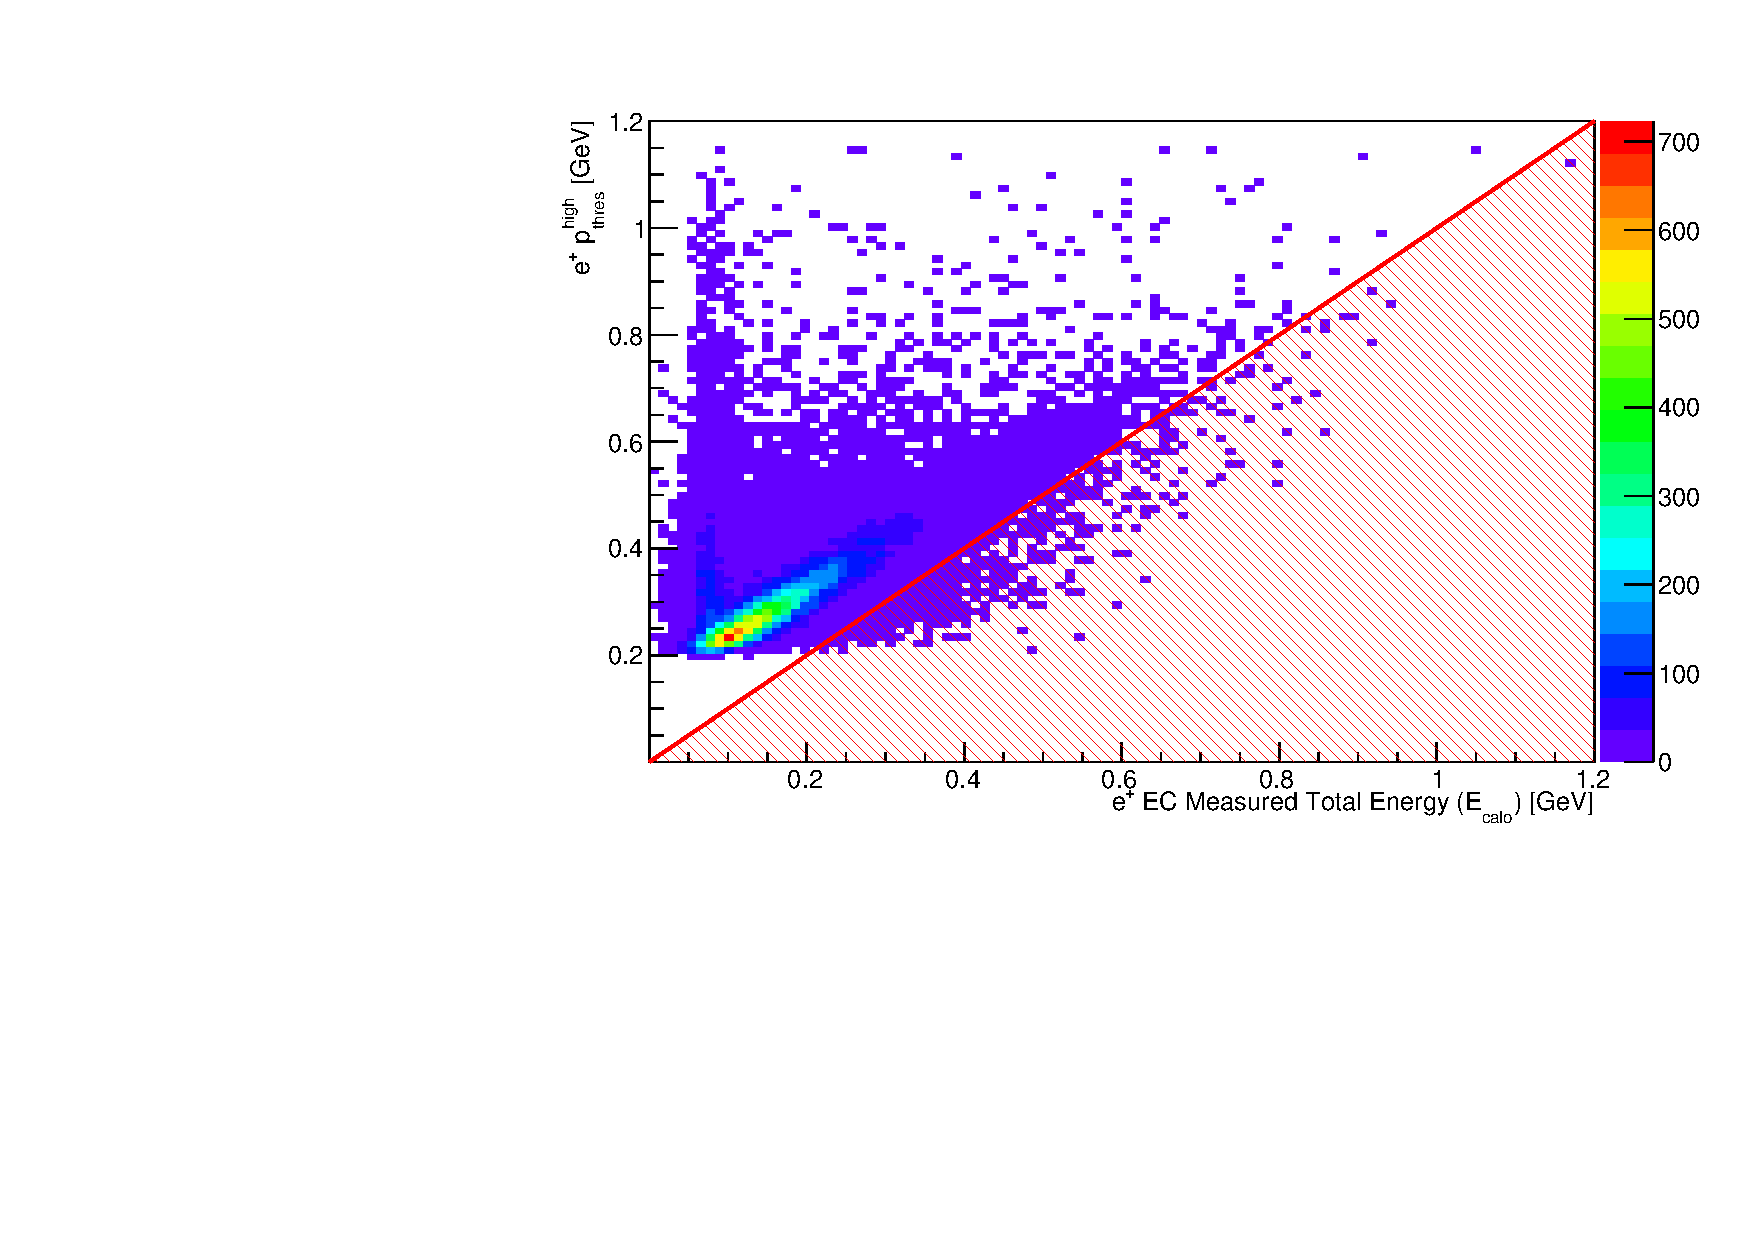
\includegraphics[width=\figwidth,height=0.7\hfigheight]{\figures/analysis/LEP_FEATURES/Pip_EChighcut.pdf}
\caption[\abbr{EC} Deposited Energy Comparison to Track Momentum for e$^+$ from \piz Events]{\label{fig:islep.pipECcut}Plot of energy deposited measured by \abbr{EC} vs. track momentum p$\mathrm{_{thres}^{high}}$ for positrons from \piz events without the \emph{g7} lepton \abbr{EC} \abbr{PID} scheme applied. The red region depicts the cut that would reject events in the \emph{g7} lepton \abbr{EC} \abbr{PID} scheme.}
\end{center}\end{figure}
%


\FloatBarrier



\section{\g12 Corrections}\label{sec:analysis.corrections}
There were three corrections that were implemented onto the \g12 data set. The first correction was applied to the tagger subsystem due to a magnetic field problem that affected only the \g12 experiment. The second correction corrects for the ``energy-loss'' of a particle through matter. These corrections are discussed further in the proceeding subsections. The third correction was the tagger sag correction that was handled in the tagger calibration.
\subsection{Energy Loss}\label{sec:analysis.corrections.eloss}

Since tracking began after the particle had already traversed through the target and \abbr{ST}, the measured momentum was decreased by the ``energy-loss'' the particle underwent before entering the Region 1 \abbr{DC}. This ``energy-loss' is due to charged particles losing their energy through atomic excitation and ionization while traveling through materials in the \abbr{CLAS} detector. The effect of ``energy-loss'', in \abbr{CLAS}, is only indicative to all charged particles. However, using the Bethe-Bloch equation:
\begin{align}
\frac{dE}{dx} \sim \frac{\ln \gamma}{\beta^2} \ ,
\end{align}
where $\gamma$ and $\beta$ have their usual meanings, it is seen that for electrons with $\beta \approx 1$ lose less energy than protons. Therefore ``energy-loss" corrections are not applied to electrons or positrons. For those charged particles that are subject to ``energy-loss'', such as the proton for this analysis, corrections were made to account for energy lost in the target material ($\ell H_2$), kapton target walls, the beam pipe, the start counter and the air between the start counter and the Region 1 \abbr{DC}. The corrections were applied by the eloss software package written by Eugene Pasyuk for the CLAS detector~\cite{clas.eloss} as an add-on to the \abbr{CLASEVENT} software package.

\subsection{Beam Corrections}\label{sec:analysis.corrections.beam}
Initially, missing masses computed for \g12 were systematically low. It was realized while investigating the issue that the low missing mass depended on run number and varied by as much as 10~MeV. The run dependent missing mass showed a constant low mass (run$<$56550) followed by a higher mass which remained constant (56500$<$run$<$56920) until another increase in mass (run$>$56920). To analyze and correct for the problem, two reactions were chosen to select missing protons and neutrons. The first reaction;
\begin{equation}
\gamma p \rightarrow \pi^+ \pi^- p \label{eq:beam.cortopology}
\end{equation}
was used to derive the correction, while the second reaction;
\begin{align}
\gamma p \rightarrow \pi^+ \pi^+ \pi^- (n)  \label{eq:beam.checktopology}
\end{align}
was chosen to verify the corrections. The reaction of Eq.~\ref{eq:beam.cortopology} was used to derive the correction because all three particles can be detected. Thus
\begin{align}
(P_{\gamma} + P_{target} - (P_{\pi^+} + P_{\pi^-}))^2 = P^2_{p} = m_p^2 \,
\end{align}
where $P_{\gamma}$, $P_{target}$,$P_{\pi^{\pm}}$ and $P_{p}$ are the 4-vectors of the incident photon, target, $\pi^{\pm}$ and proton respectively and $m_p$ is the mass of the proton.
We selected events for the correction with one \abbr{CLAS} \abbr{PID} $\pi^+$, one \abbr{CLAS} \abbr{PID} $\pi^-$, one \abbr{CLAS} \abbr{PID} proton and nothing else. Exclusive cuts were then placed by requiring the missing energy, $M_E(\gamma p \rightarrow p \pi^+ \pi^-) < 0.025$~GeV and the missing mass squared of $M_x^2(\gamma p \rightarrow p \pi^+ \pi^-) < 0.015$~GeV$^2$. These cuts assure that the selected evetns did not have a undetected $pi^0$,
since the mass squared of \piz $= 0.0182$~GeV$^2$.

The first step chosen was to verify whether the ``energy-loss'' correction was causing the discrepancy,. This can be seen in Figs.~\ref{fig:beamcor.p_mass},~\ref{fig:beamcor.n_mass}. It was concluded that the ``energy-loss'' correction was not the problem. From Fig.~\ref{fig:beamcor.p_mass}, two runs were chosen, 56515 and 57130, in which the difference in the missing mass was $\approx$10~MeV. Inspecting the invariant mass, $M(\pi^+\pi^-)$, Fig~\ref{fig:beamcor.k_mass}, for runs 56515 and 57130 revealed only a mass deviation of $\approx$1.4~MeV. This implies that the problem  is caused by the photon beam energy.


\begin{figure}[h!]\begin{center}
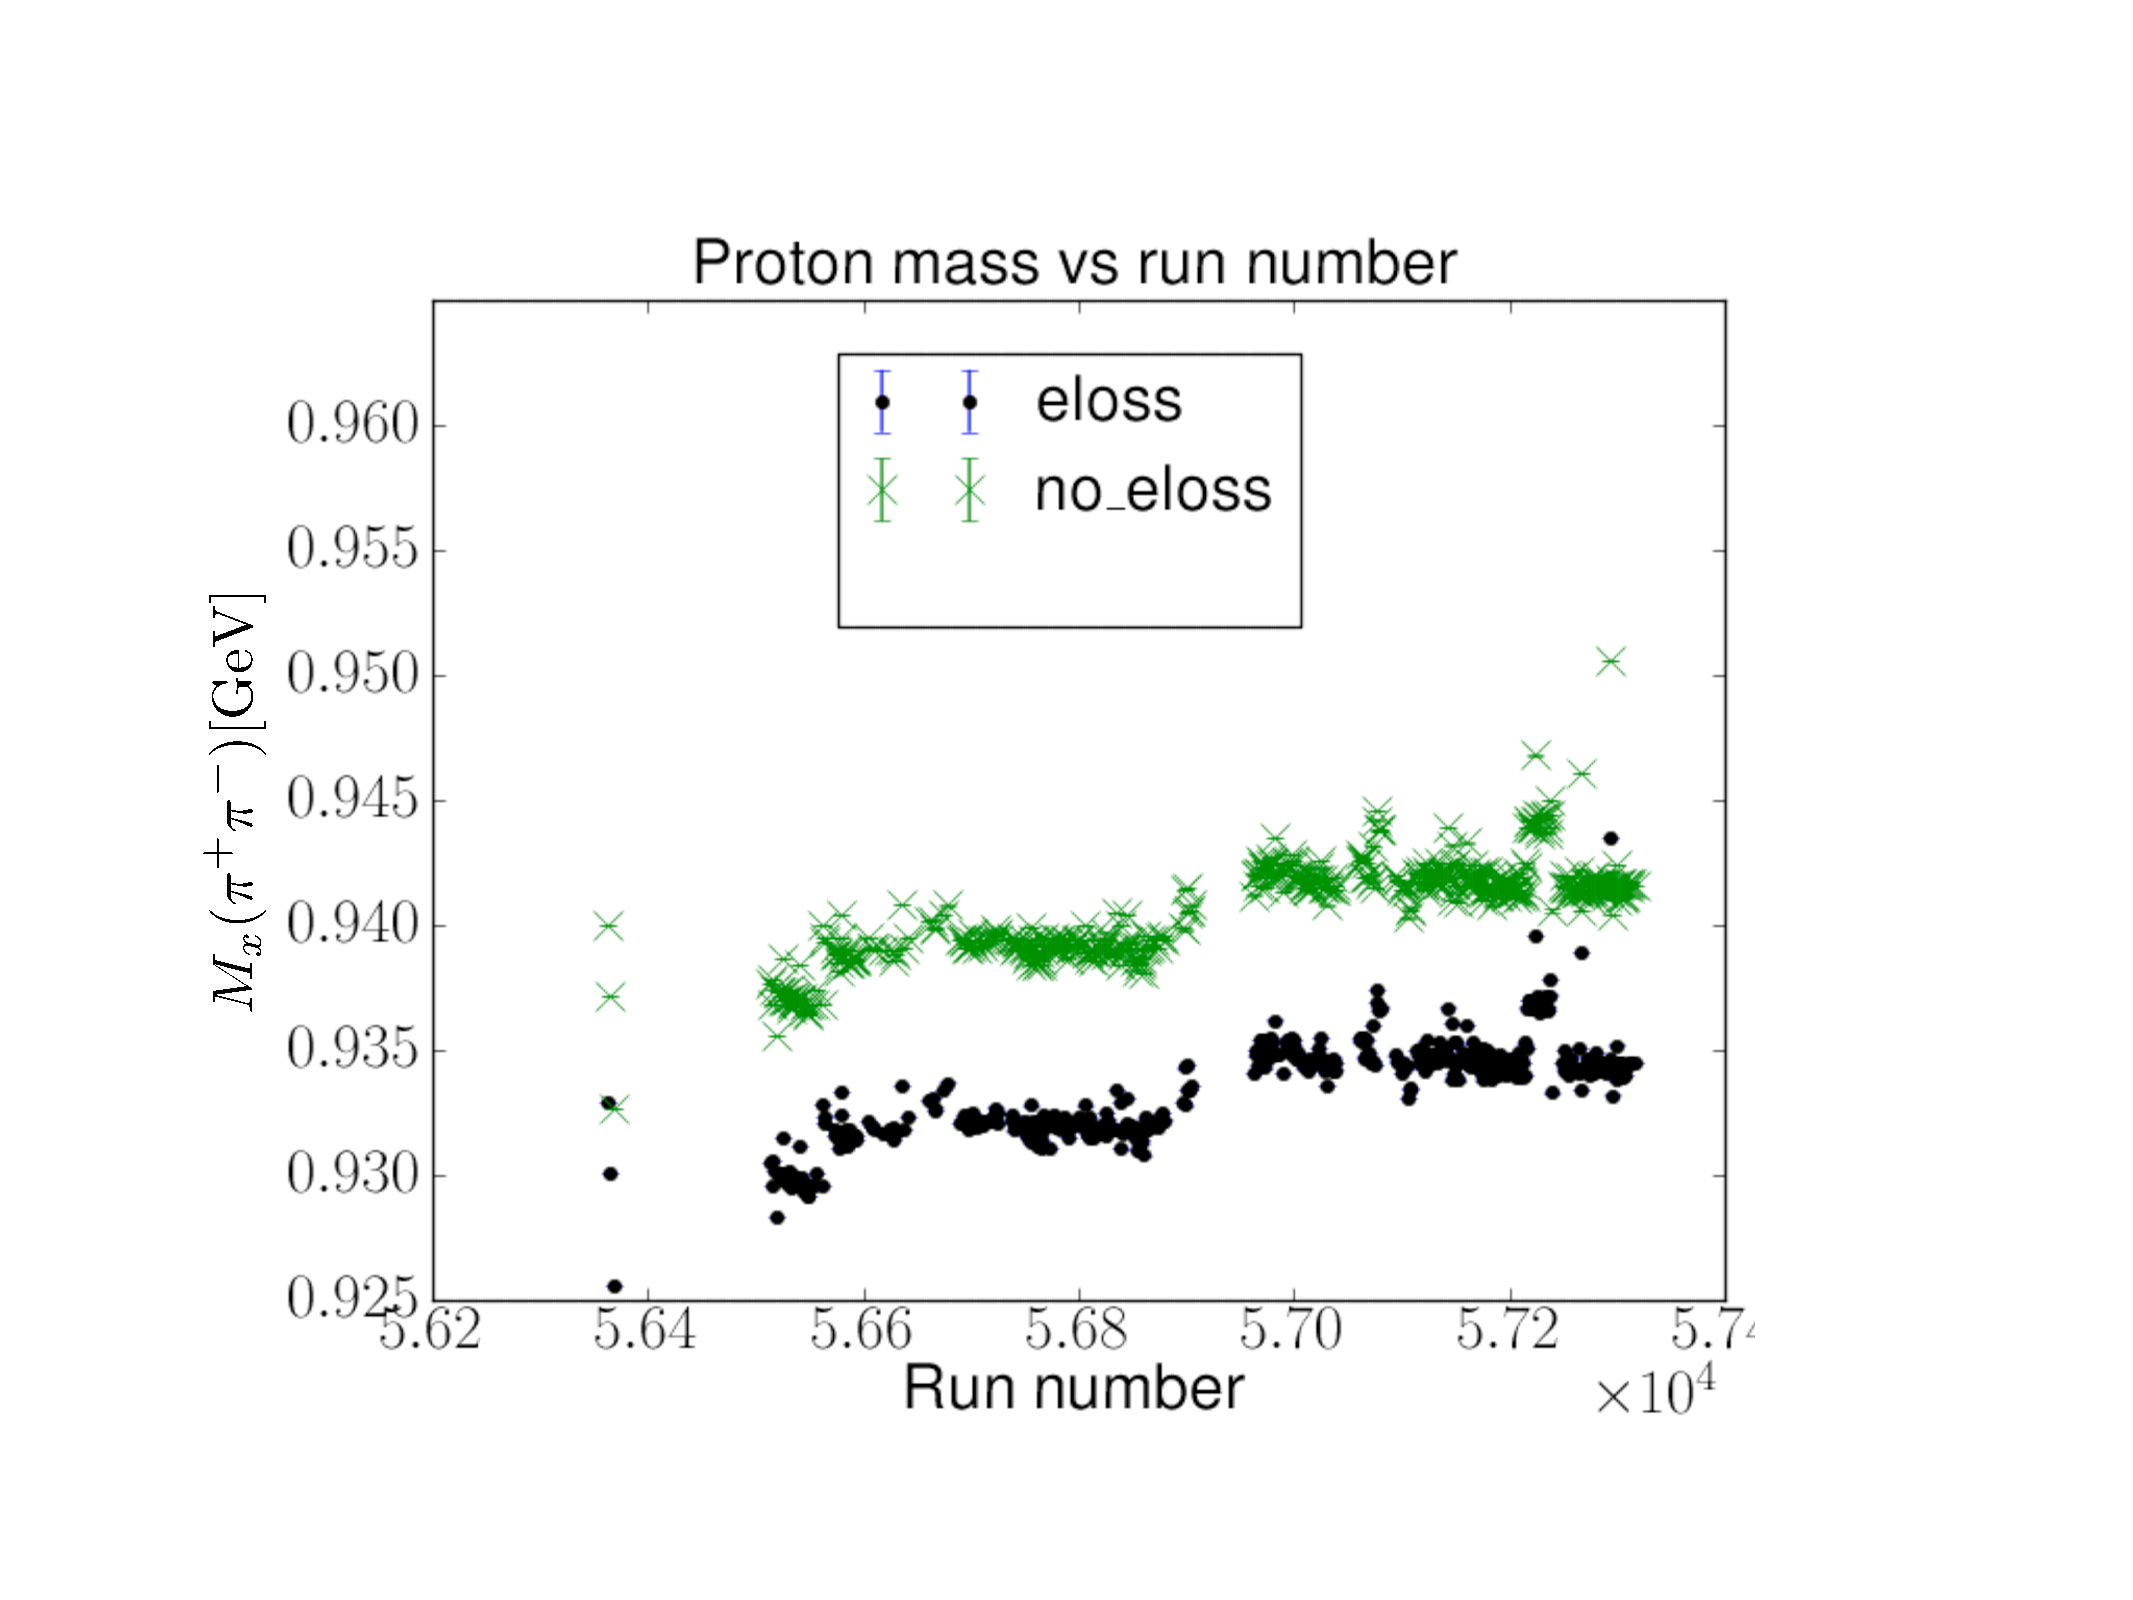
\includegraphics[width=\figwidth,height=0.75\hfigheight]{\figures/analysis/beam_correction/P_mass_issue.pdf}
\caption[Plot of \g12 run number vs. undetected proton mass with and without the ``energy-loss'' applied]{\label{fig:beamcor.p_mass}Plot of \g12 run number vs. undetected proton mass with and without the ``energy-loss'' applied. }
\end{center}\end{figure}

\begin{figure}[h!]\begin{center}
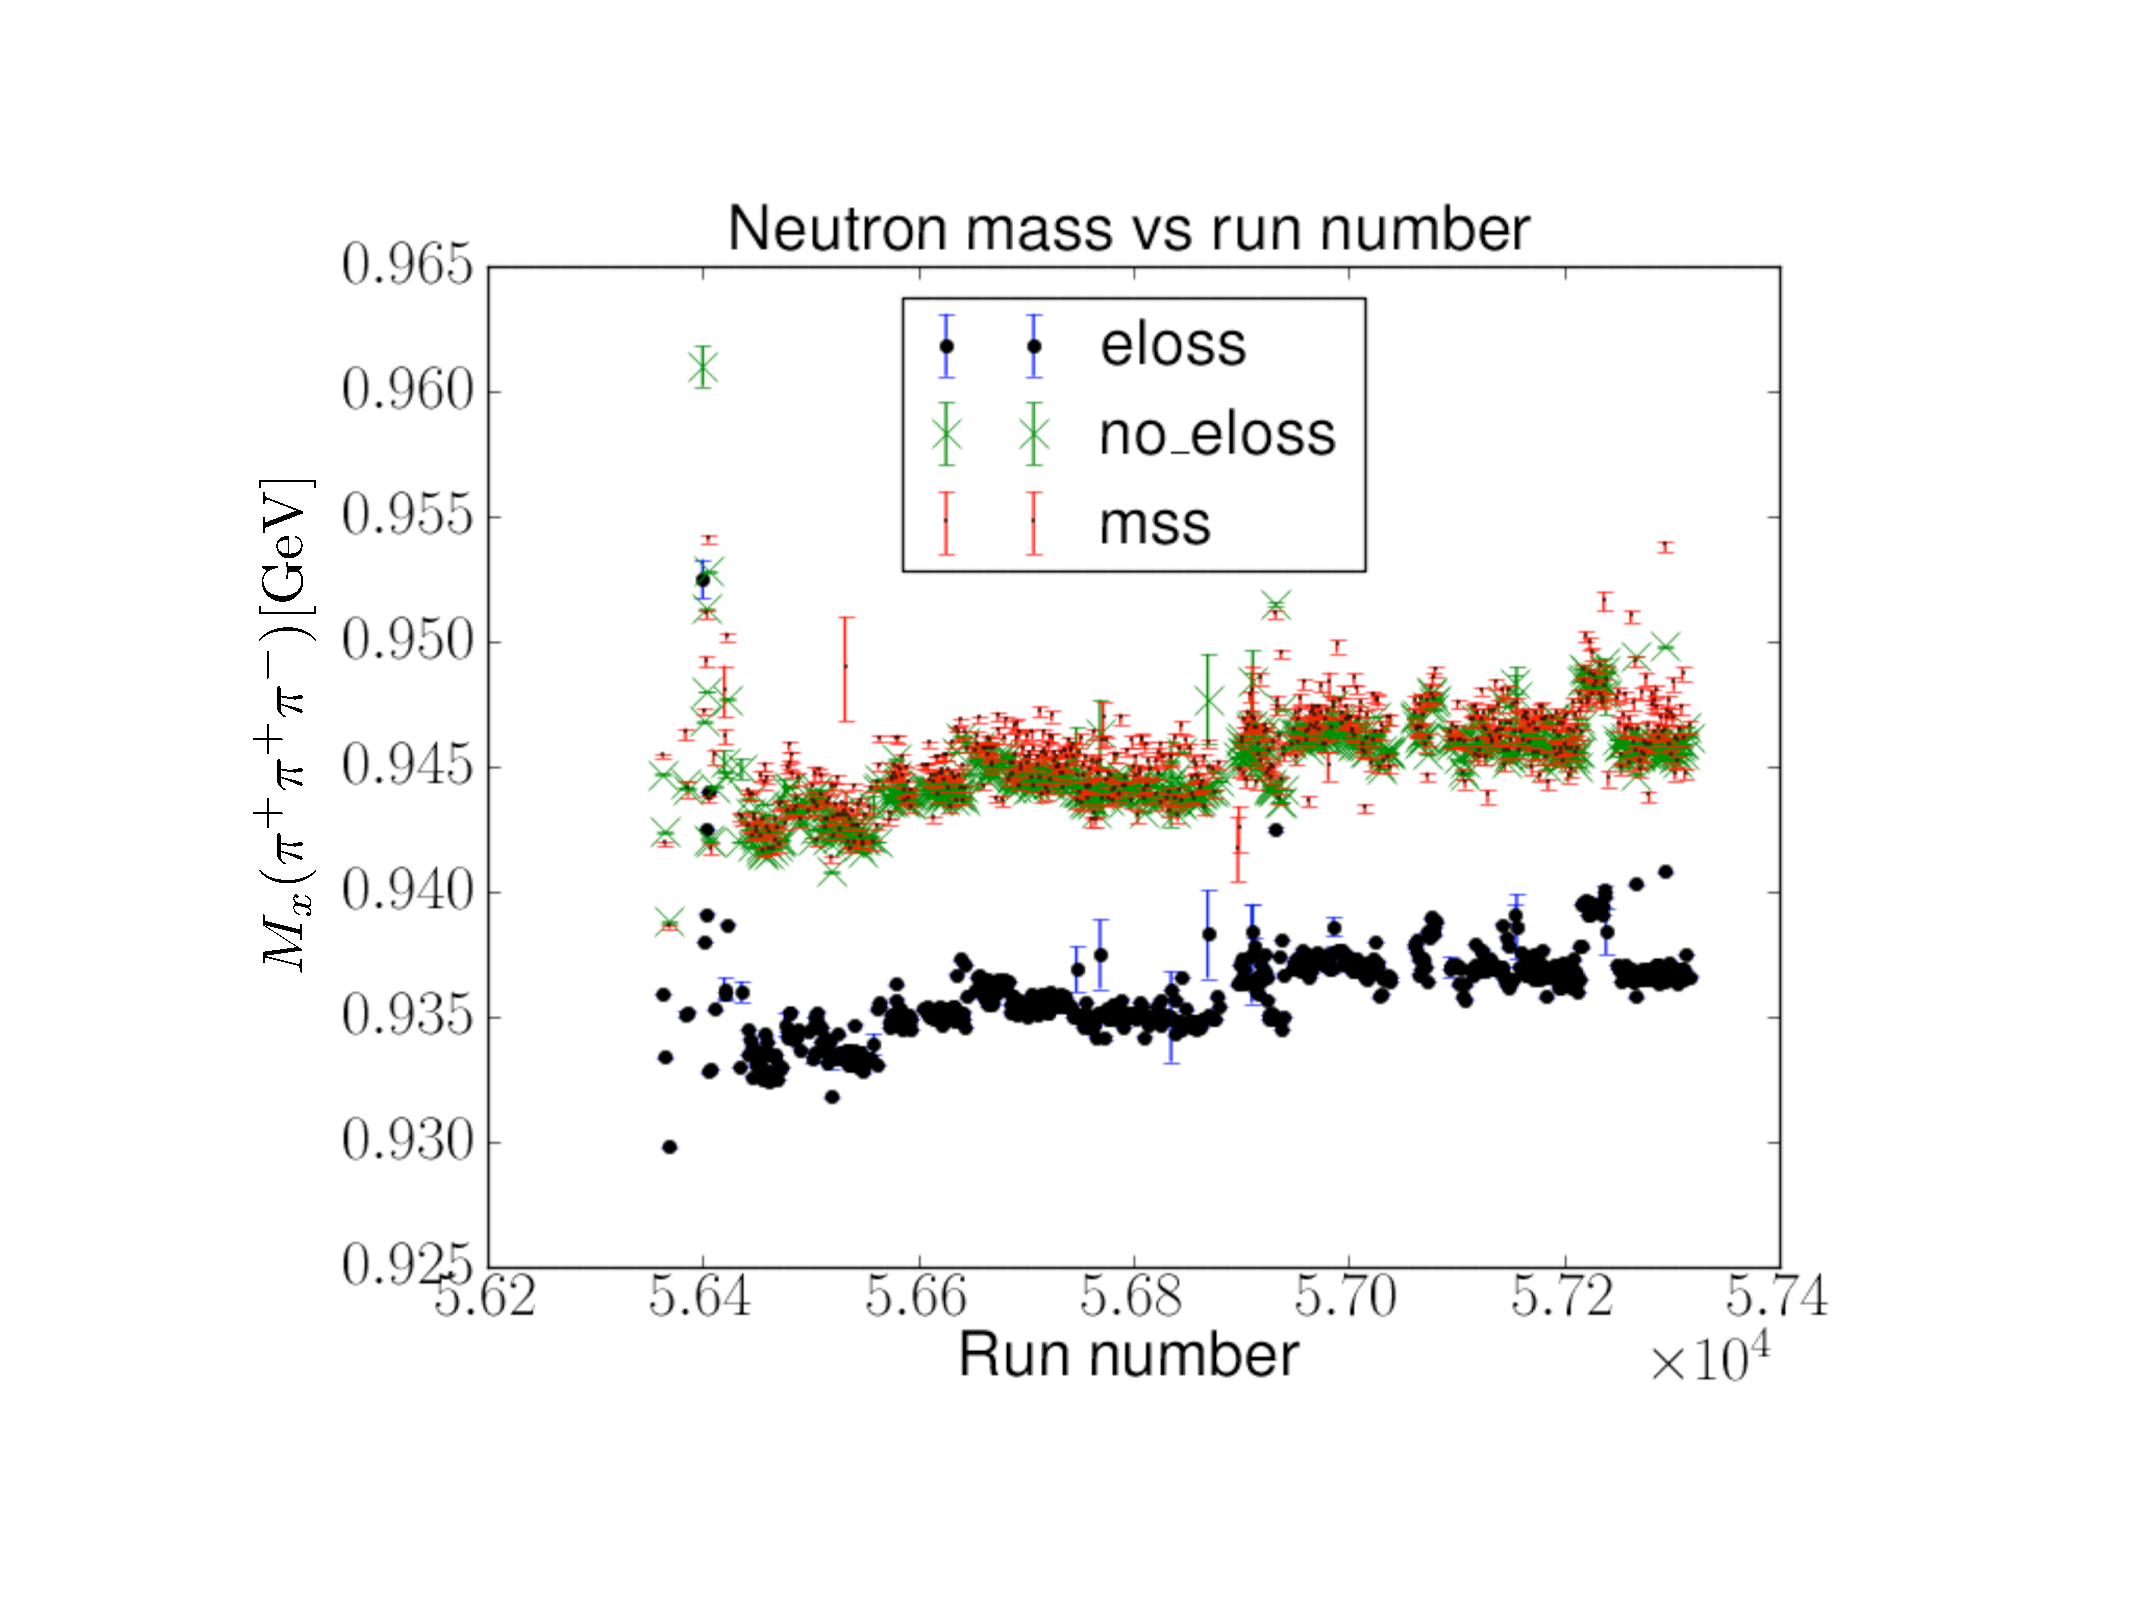
\includegraphics[width=\figwidth,height=0.75\hfigheight]{\figures/analysis/beam_correction/N_mass_issue.pdf}
\caption[Plot of \g12 run number vs. undetected neutron mass with and without the ``energy-loss'' applied]{\label{fig:beamcor.n_mass}Plot of \g12 run number vs. undetected neutron mass with and without the ``energy-loss'' applied. The red data points labeled ``mss" are data taken directly from tape. Image Source:~\cite{bookwalter}}
  \end{center}\end{figure}
  
  \begin{figure}[h!]\begin{center}
  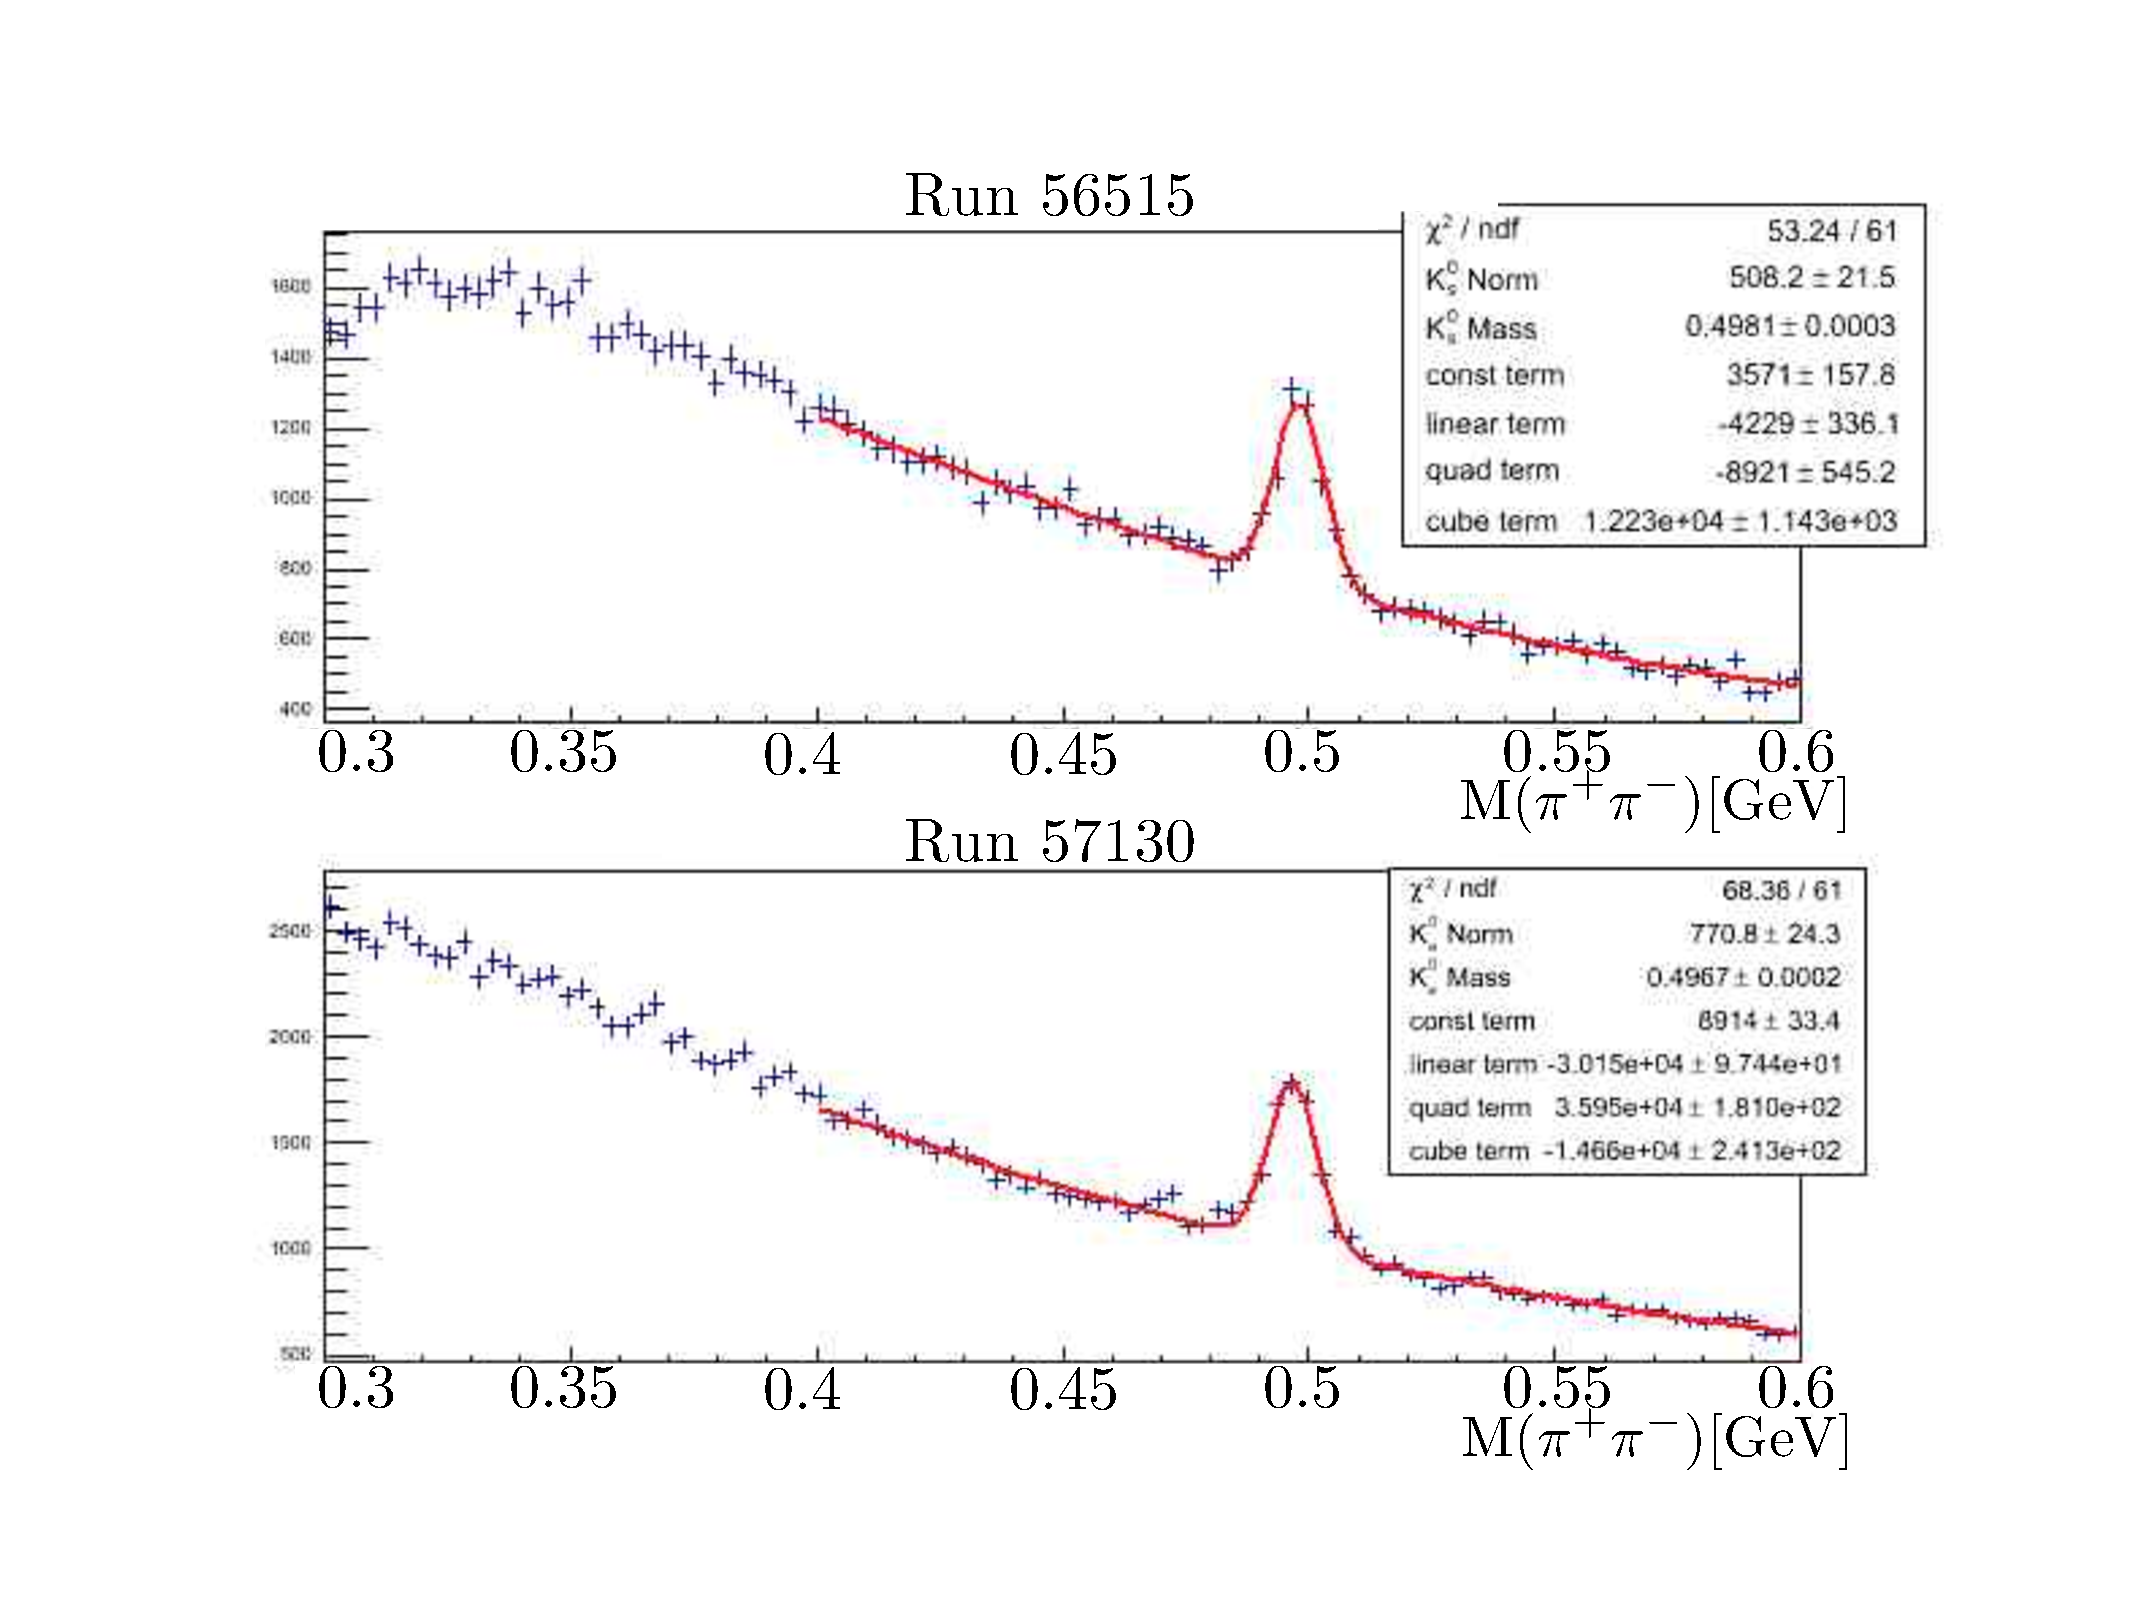
\includegraphics[width=\figwidth,height=0.7\hfigheight]{\figures/analysis/beam_correction/Kaon_mass.pdf}
  \caption[Plot of $\pi^+ \pi^-$ mass for runs 56515 and 57130]{\label{fig:beamcor.k_mass}Plot of $\pi^+ \pi^-$ mass for runs 56515 and 57130. $m_{K_0}$ = 0.4976 GeV/c$^2$.}
  \end{center}\end{figure}
  % % %
  \FloatBarrier
  Several tagger quantities were analyzed. The tagger magnet current was apparently constant (see Fig.~\ref{fig:tag.magnet.epics}) but had been turned off around run=56920 (May 12, 2008). When the tagger magnet was turned on, the current was set to its previous setting. The tagger magnet current was recorded by the accelerator group shown in Fig.~\ref{fig:tag.magnet.arne}, it was also stable throughout the running of \g12. The beam current was also stable (see Fig.~\ref{fig:beamcurrents})
  
  %Now that it is known that the photon beam energy is the cause of the issue, it must be known the cause of the photon beam error. Several quantities that the tagger subsystem are subjected to were analyzed, first being the tagger magnet current which, according to the \abbr{EPICS} Fig~\ref{fig:tag.magnet.epics}, remain constant
  %but showed that around run = 56920 (May 12, 2008) the tagger magnet was shut-off. The tagger magnet shut-off was done because work had to be done in the hall, however after the tagger magnet was turned on, the current was set to its previous setting. A further investigation into the tagger magnet was performed by private communication with the accelerator group chief Arne Freyberger, Fig~\ref{fig:tag.magnet.arne} shows the data the accelerator group had for the tagger magnet which confirms that the tagger magnet current was stable throughout the running of \g12. The next beam quantity analyzed was the beam current delivered by \abbr{CEBAF}, again through private communication with the accelerator group chief Arne Freyberger it is shown in Fig.~\ref{fig:beamcurrents} that the electron beam current remained constant throughout the \g12 experiment.
  
  \begin{figure}[h!]\begin{center}
  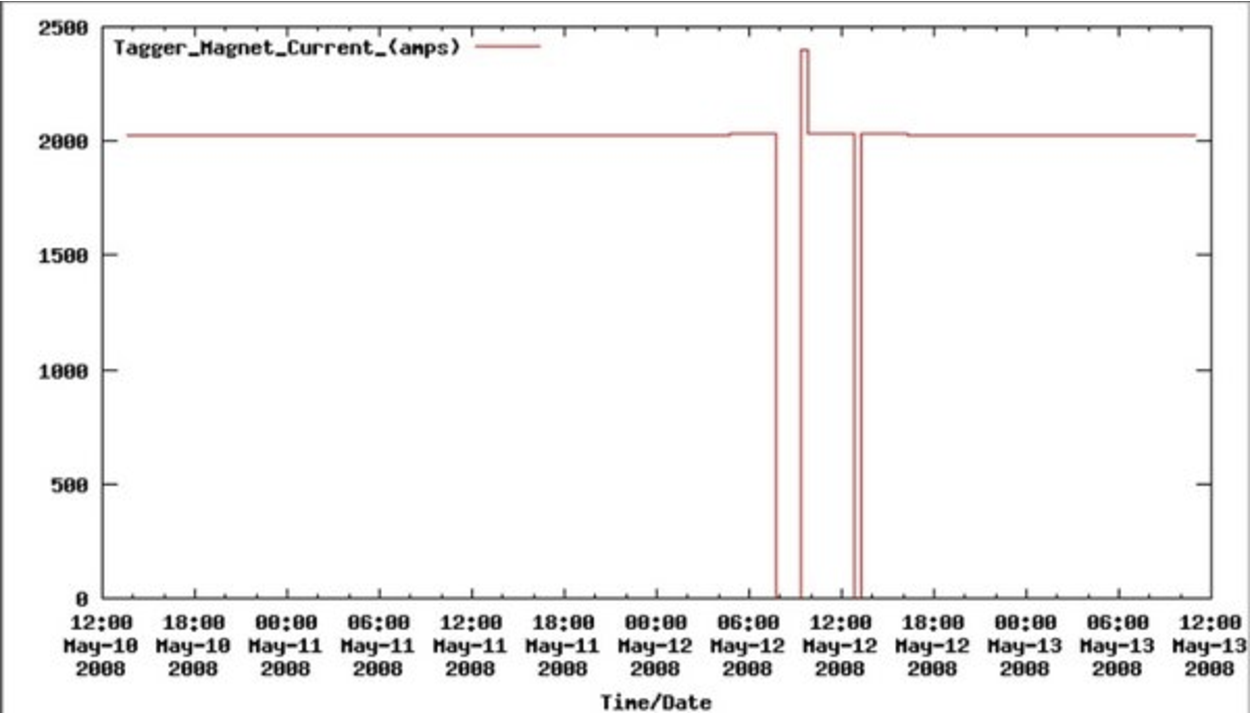
\includegraphics[width=\figwidth,height=0.7\hfigheight]{\figures/analysis/beam_correction/600px-Hystersis_smokingGun.pdf}
  \caption[Tagger magnet current according to \abbr{EPICS}]{\label{fig:tag.magnet.epics}Tagger magnet current according to \abbr{EPICS}}
  \end{center}\end{figure}
  
  \begin{figure}[h!]\begin{center}
  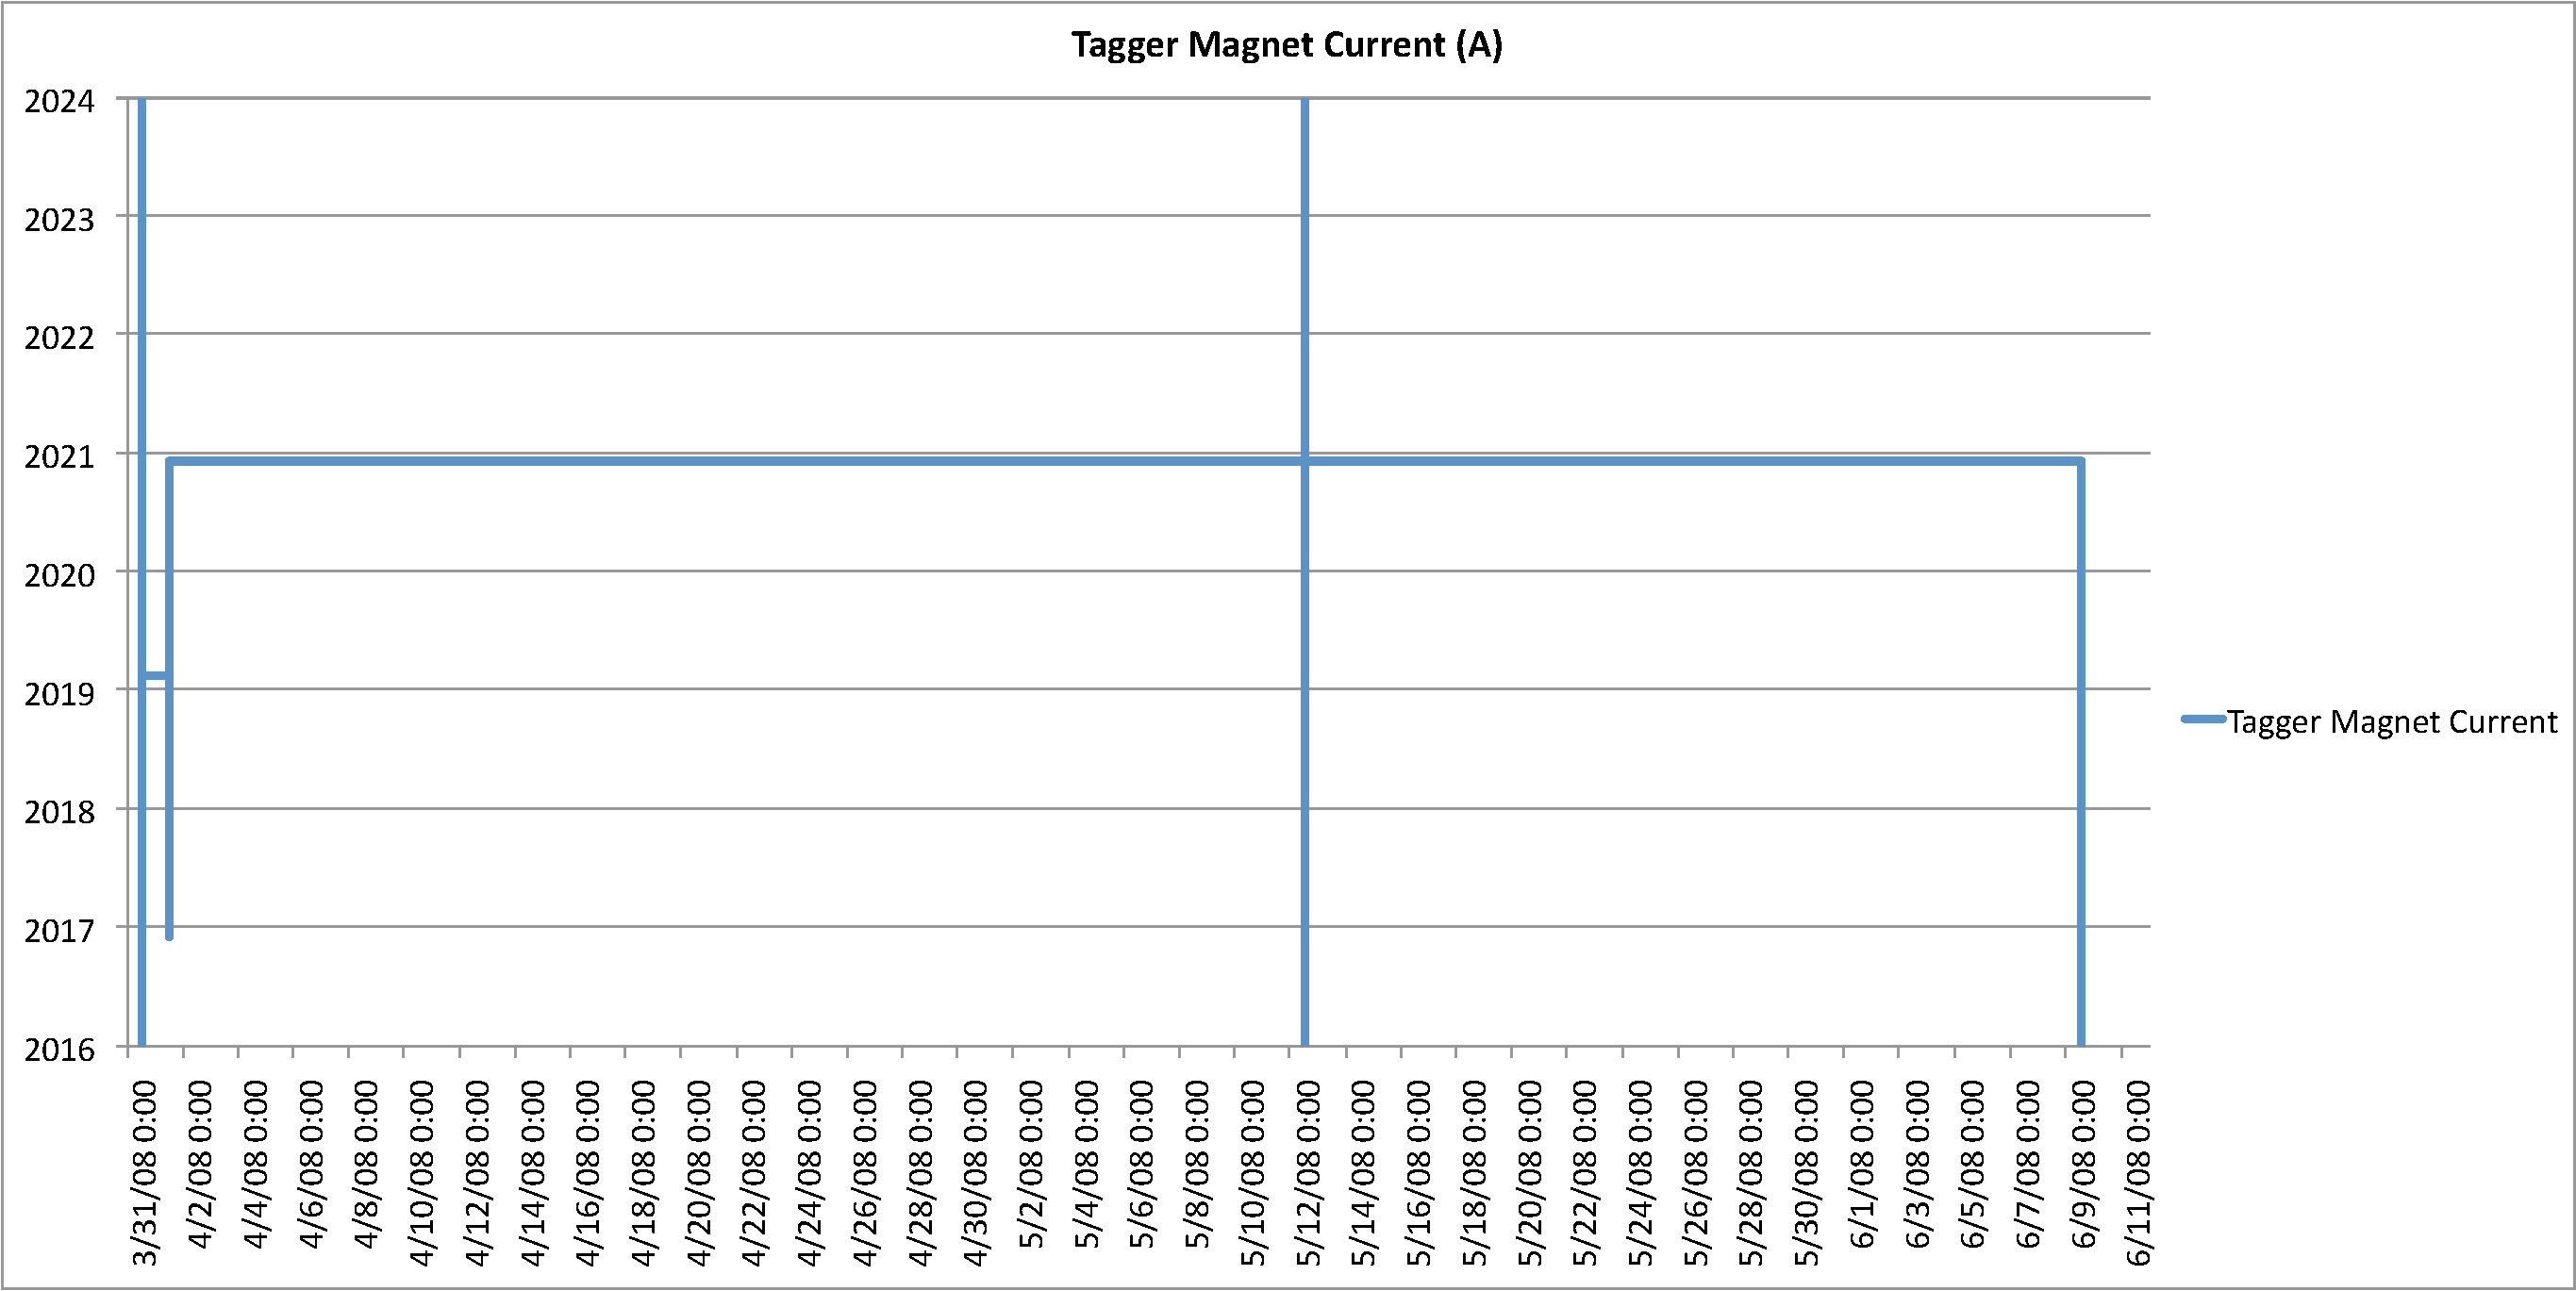
\includegraphics[width=\figwidth,height=0.7\hfigheight]{\figures/analysis/beam_correction/tagger_current_arne.pdf}
  \caption[Tagger magnet current according to accelerator group via \abbr{EPICS}]{\label{fig:tag.magnet.arne} Tagger magnet current according to accelerator group via \abbr{EPICS}}
  \end{center}\end{figure}
  
  \begin{figure}[h!]\begin{center}
  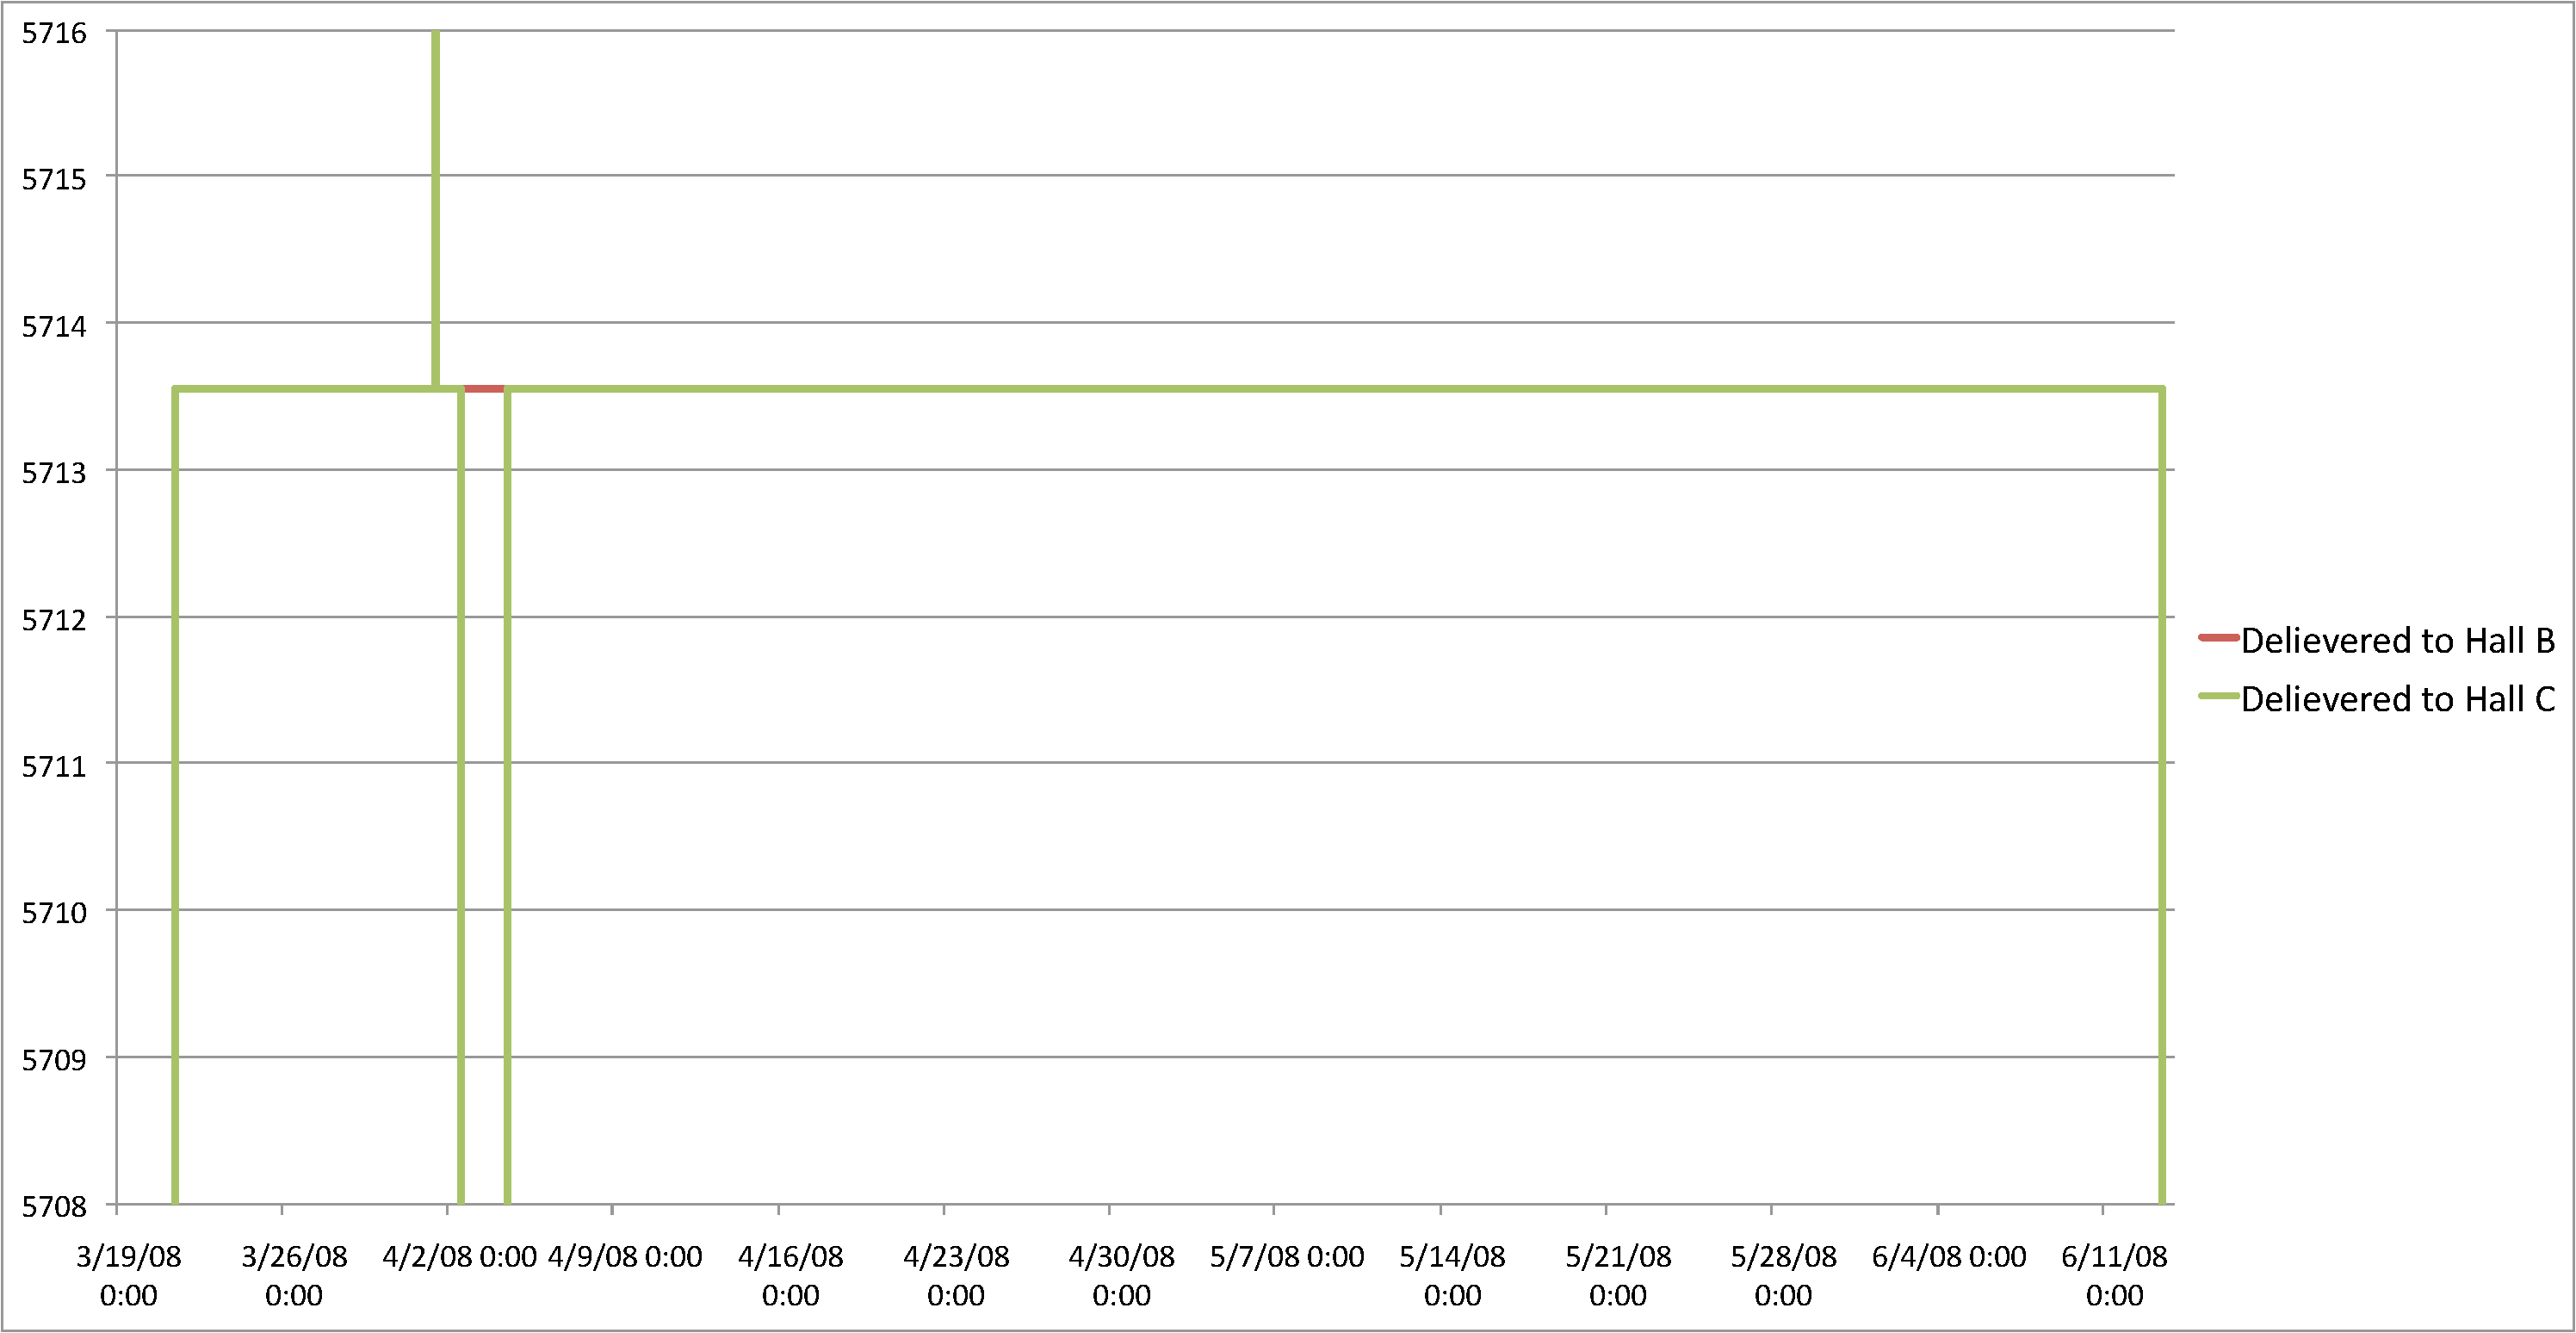
\includegraphics[width=\figwidth,height=0.7\hfigheight]{\figures/analysis/beam_correction/beam_currentsII.pdf}
  \caption[Electron beam current delivered to hall \desg{B}(red) and hall \desg{C} (green) according to the accelerator group during \g12]{\label{fig:beamcurrents}Electron beam current delivered to hall \desg{B}(red) and hall \desg{C} (green) according to the accelerator group during \g12. The green line overlays the red line except during the time around April, 03, 2008.}
  \end{center}\end{figure}
  
  The next quantity investigated was the positioning of the beam spot on the tagger dump. This quantity was used in place of the tagger magnetic field strength because hall \desg{B} does not measure the tagger magnetic field strength. However since the radius of curvature of a charged particle is inversely proportional to the magnetic field this quantity is suitable.
  \begin{equation}\label{eq:motioninmagII}
  p = qrB \ (\mathrm{if}\ \vec{p} \perp \vec{B} )
  \end{equation}
  The y-position of the tagger beam spot on the dump jumps on or about May 12, 2008 (see Fig.~\ref{fig:tagdump}). The change in y-position can only be due to the magnetic field changing. The phenomena in magnetism that allows for a steady current but a change in magnetic field is known as hysteresis (see Fig.~\ref{fig:hyst}).
    \begin{figure}[h!]\begin{center}
  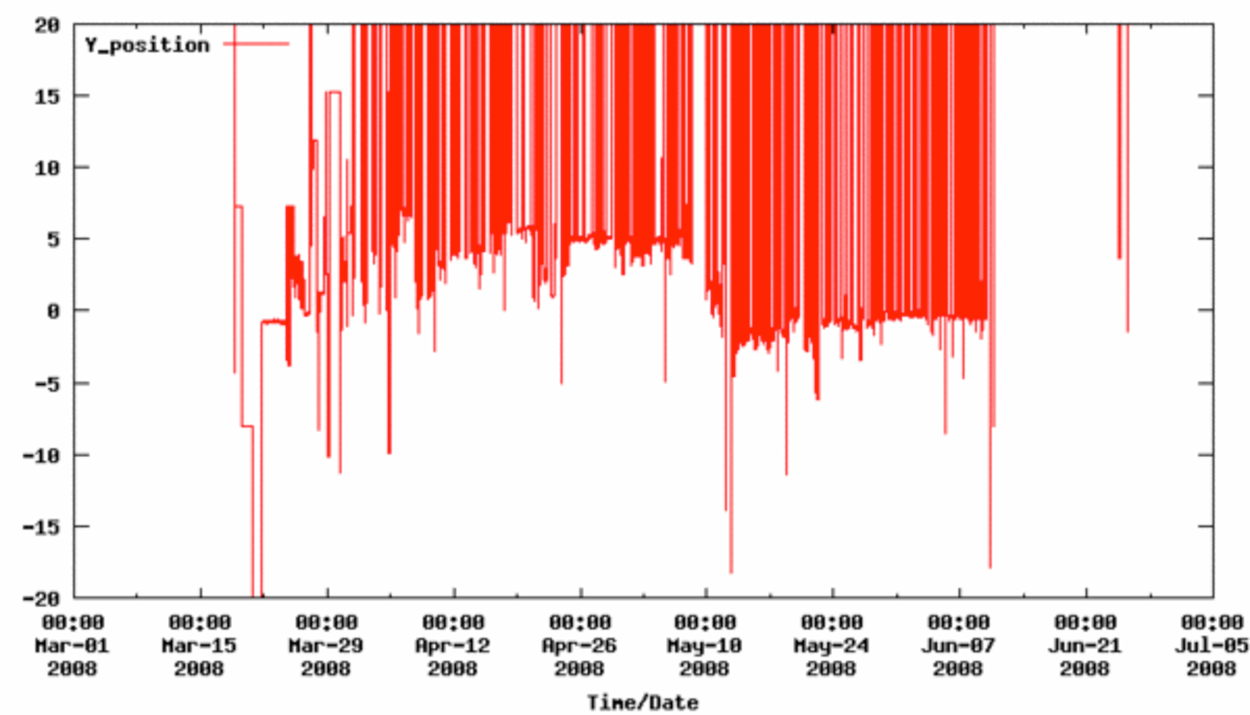
\includegraphics[width=\figwidth,height=0.7\hfigheight]{\figures/analysis/beam_correction/600px-Tagger-dump-y.pdf}
  \caption[Tagger dump beam spot y-position according to \abbr{EPICS}]{\label{fig:tagdump}Tagger dump beam spot y-position according to \abbr{EPICS}}
  \end{center}\end{figure}
  
  \begin{figure}[h!]\begin{center}
  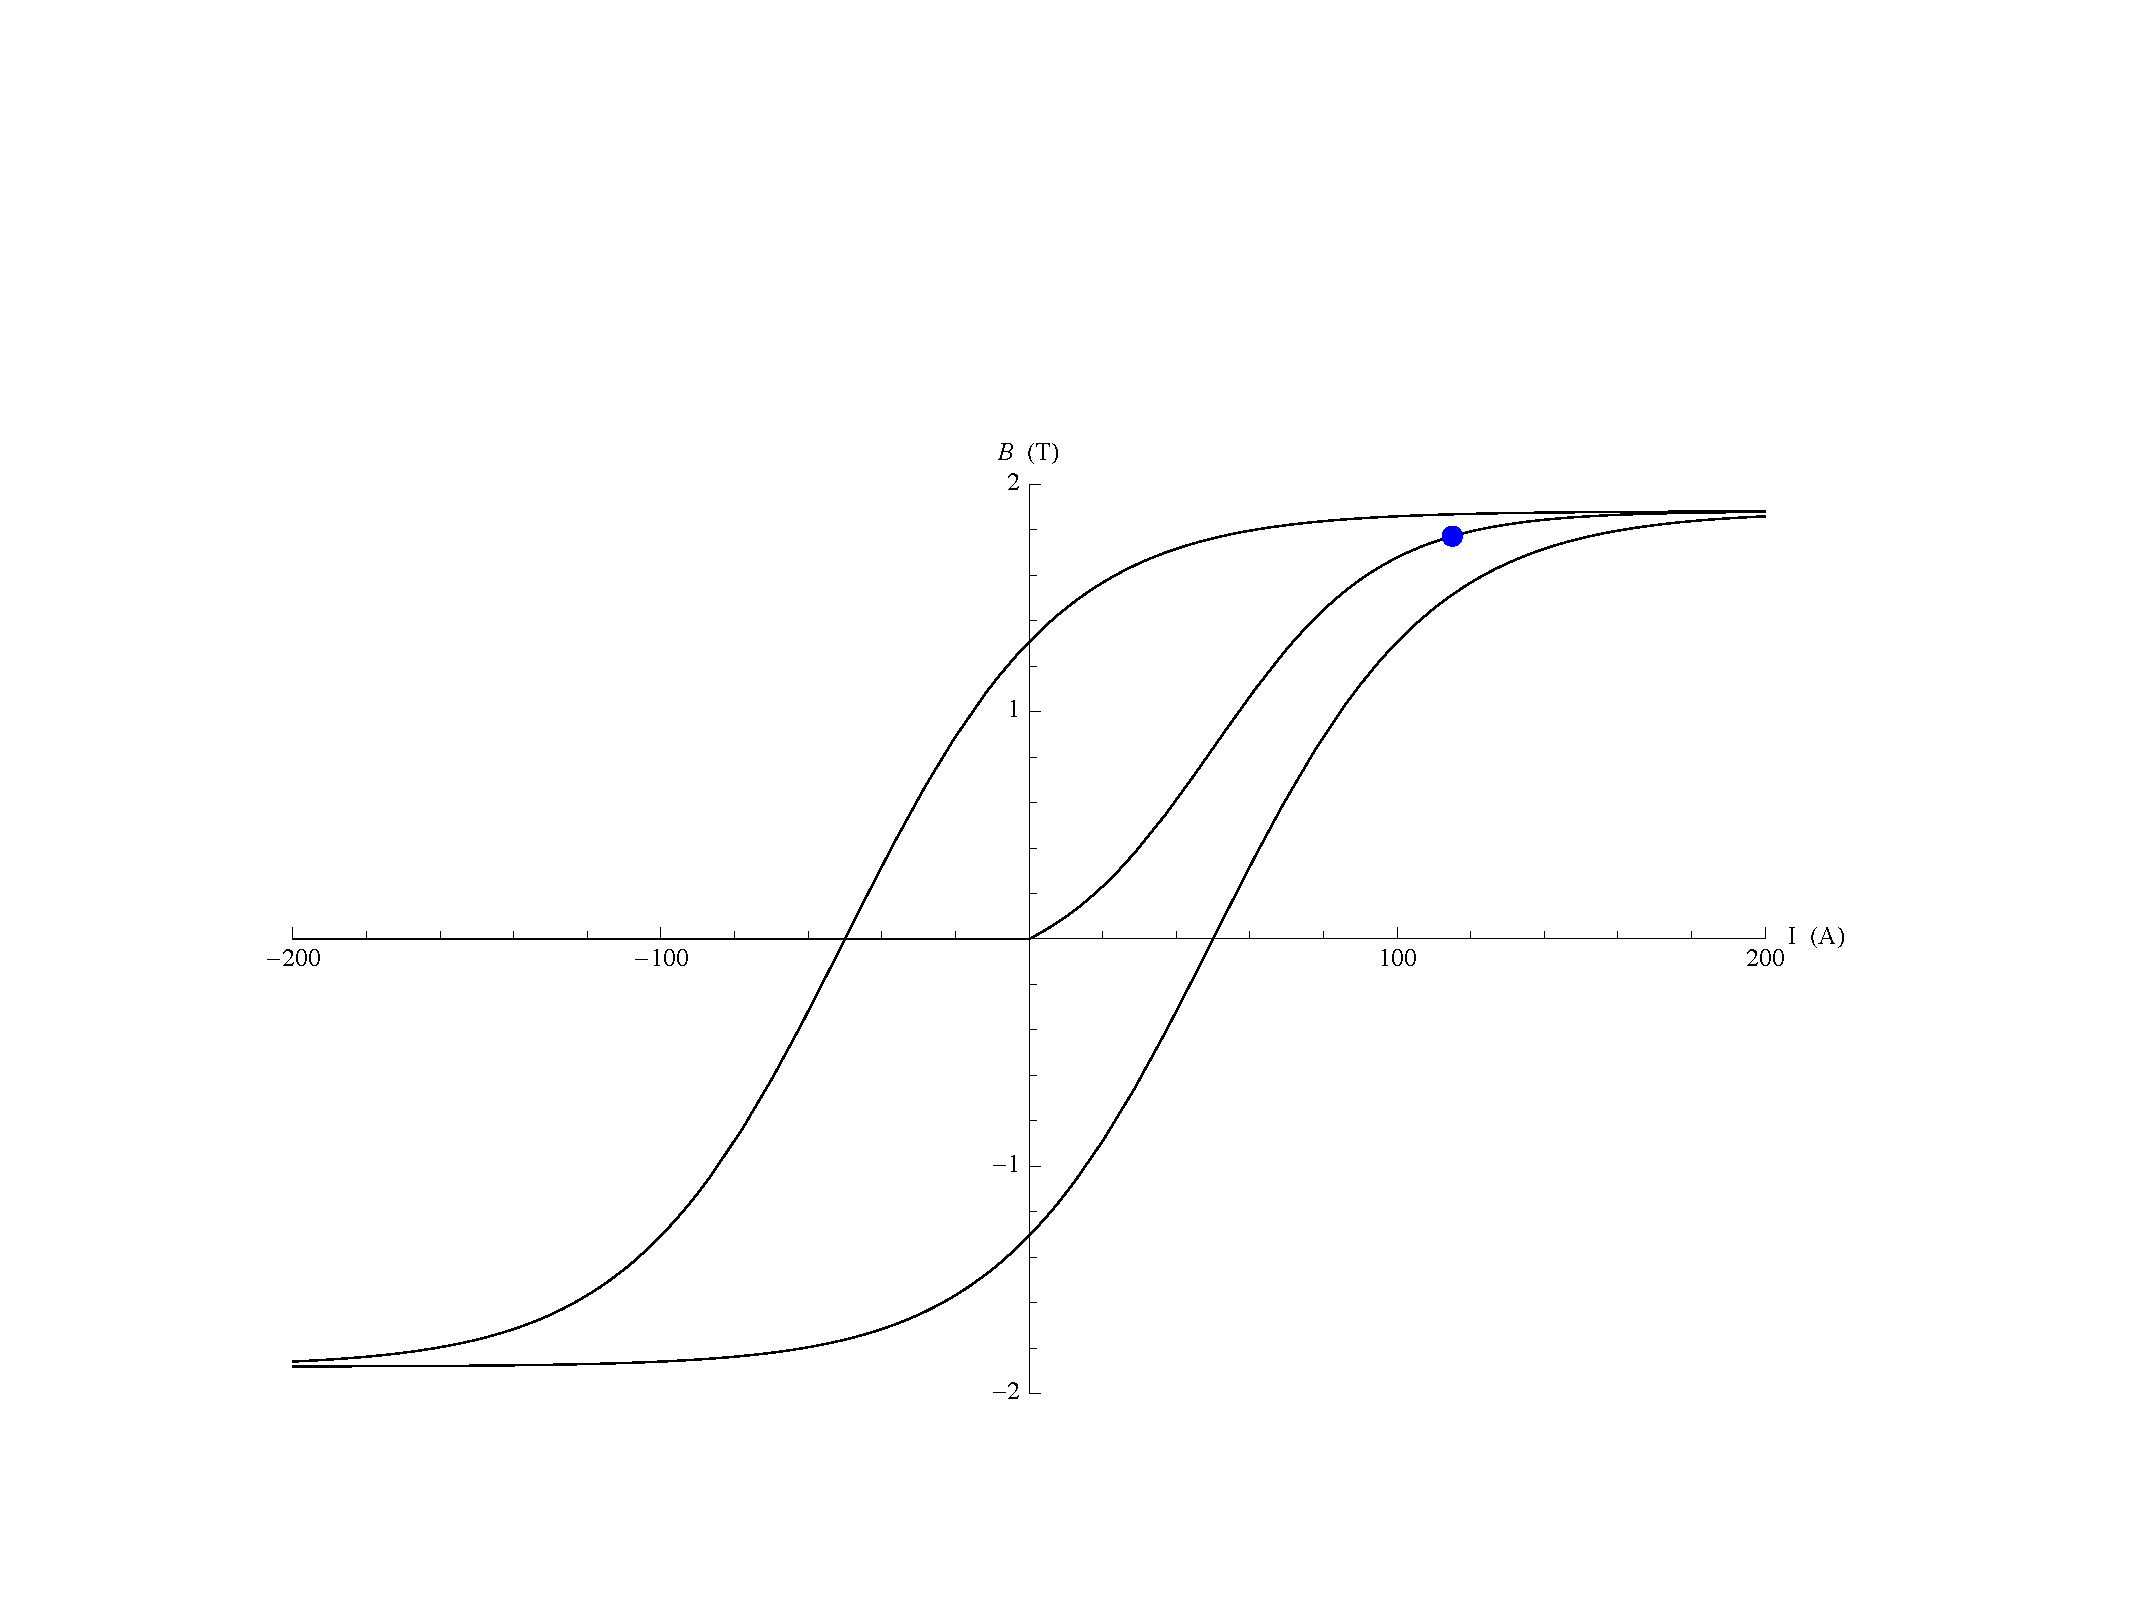
\includegraphics[width=\figwidth,height=0.7\hfigheight]{\figures/analysis/beam_correction/hysteresis_keynote.pdf}
  \caption[Plot depicting magnetic field strength vs. magnet current showing the process of hysteresis]{\label{fig:hyst}Plot depicting magnetic field strength vs. magnet current showing the process of hysteresis. For a current of strength I, there could exist many magnetic fields of strength B.}
  \end{center}\end{figure}
  \FloatBarrier
  It appeared that the \g12 missing mass fluctuations are due to tagger magnet hysteresis and the effect it would be on the scattered electron nd hence the tagged photon. The tagged photon energies were corrected as follows;
  \begin{align}
  P_{\pi^+} + P_{\pi^-} = P_{\pi^+ \pi^-} \nonumber
  \end{align}
  where $P_{\pi^+}$, $P_{\pi^-}$ are the 4-momenta of the $\pi^+$, $\pi^-$ respectively and $P_{\pi^+ \pi^-}$ is the sum of $\pi^+$ and $\pi^-$ 4-momenta.
  Therefore;
  \begin{align}
  &(P_{\gamma} + P_{target} - (P_{\pi^+\pi^-}))^2 = m_p^2 \\
  & P_{\gamma}^2 + P_{target}^2 + P_{\pi^+\pi^-}^2 + 2P_{\gamma}P_{target} - 2P_{\gamma}P_{\pi^+\pi^-} - 2P_{target}P_{\pi^+\pi^-}= m_p^2
  \end{align}
  collecting terms of $P_{\gamma}$ to one side and using $P_{target}^2 = m_p^2 $ and $P_{\gamma}^2 = 0$
  \begin{align}\label{eq:hyst.eqI}
  P_{\pi^+\pi^-}^2 - 2P_{target}P_{\pi^+\pi^-}= 2P_{\gamma}(P_{\pi^+\pi^-} - P_{target})
  \end{align}
  From this using Eq.~\ref{eq:tagger.energy} in 4-vector notation
  \begin{align}\label{eq:tagger.energyII}
  P_{\gamma} = P_{E_0} - P_{e}\nonumber
  \end{align}
  where $P_{E_0}$ is the four vector of the incident electron and $P_{e}$ is the four vector of the scattered electron in the bremsstrahlung process that is measured by the tagger. Applying a scaler correction to $P_{e}$ as $xP_{e}$ and solving for $x$ for all known quantities, Eq.~\ref{eq:hyst.eqI} simplifies to;
  \begin{align}
  x= \frac{P_{E_0}(P_{target}-P_{\pi^+\pi^-}) + P_{\pi^+\pi^-}^2/2  - P_{target}P_{\pi^+\pi^-}}{(P_{E_0} - P_{\gamma})(P_{target} - P_{\pi^+\pi^-})}
  \end{align}
  To reduce statistical fluctuations $\frac{1}{10}$ of run 56515 was analyzed to obtain the correction factor $x$. The correction factor was fitted using a Gaussian to establish an accurate measurement of the peak, this is shown in Fig~\ref{fig:56515.cor}. After the correction factor was extracted for run 56515, it was applied to both the reactions listed in Eq.~\ref{eq:beam.cortopology} and Eq.~\ref{eq:beam.checktopology} by recalculating the photon beam energy as;
  \begin{align}
  E_e = E_{E_0} - E_{\gamma} \nonumber \\
  E_{\gamma}^{new} = E_{E_0} - xE_e \nonumber.
  \end{align}
  Figures~\ref{fig:proton.fix},~\ref{fig:neutron.fix} illustrate the missing masses after the tagger correction and show that the new calculated missing masses are less than 1~MeV from \abbr{PDG} values. Since both the missing proton mass and missing neutron mass were adjusted properly to the correct mass by using the same beam correction factor, it shows that the correction factor is independent of reaction and therefore can be applied to all \g12 analyses. The procedure to calculate $x$ was repeated for every run in \g12, Fig~\ref{fig:beamcor.run}, with $\frac{1}{10}$ of the data used. To validate the corrections of the entire \g12 data set, the missing neutron mass was recalculated for each run, shown in  Fig.~\ref{fig:neutron.fixall}, using several correction schemes, i.e. a scheme of just ``energy-loss'' corrections, a scheme of ``energy-loss'' and momentum corrections (JTG PCor), a scheme of ``energy-loss'', momentum corrections (JTG PCor) and beam corrections (MK BeamCor) and a scheme of ``energy-loss'' and beam corrections (MK BeamCor). It can be seen in Fig.~\ref{fig:neutron.fixall} that the only scheme that sufficed was the combination of ``energy-loss'' and beam corrections.
  
  
  \begin{figure}[h!]\begin{center}
  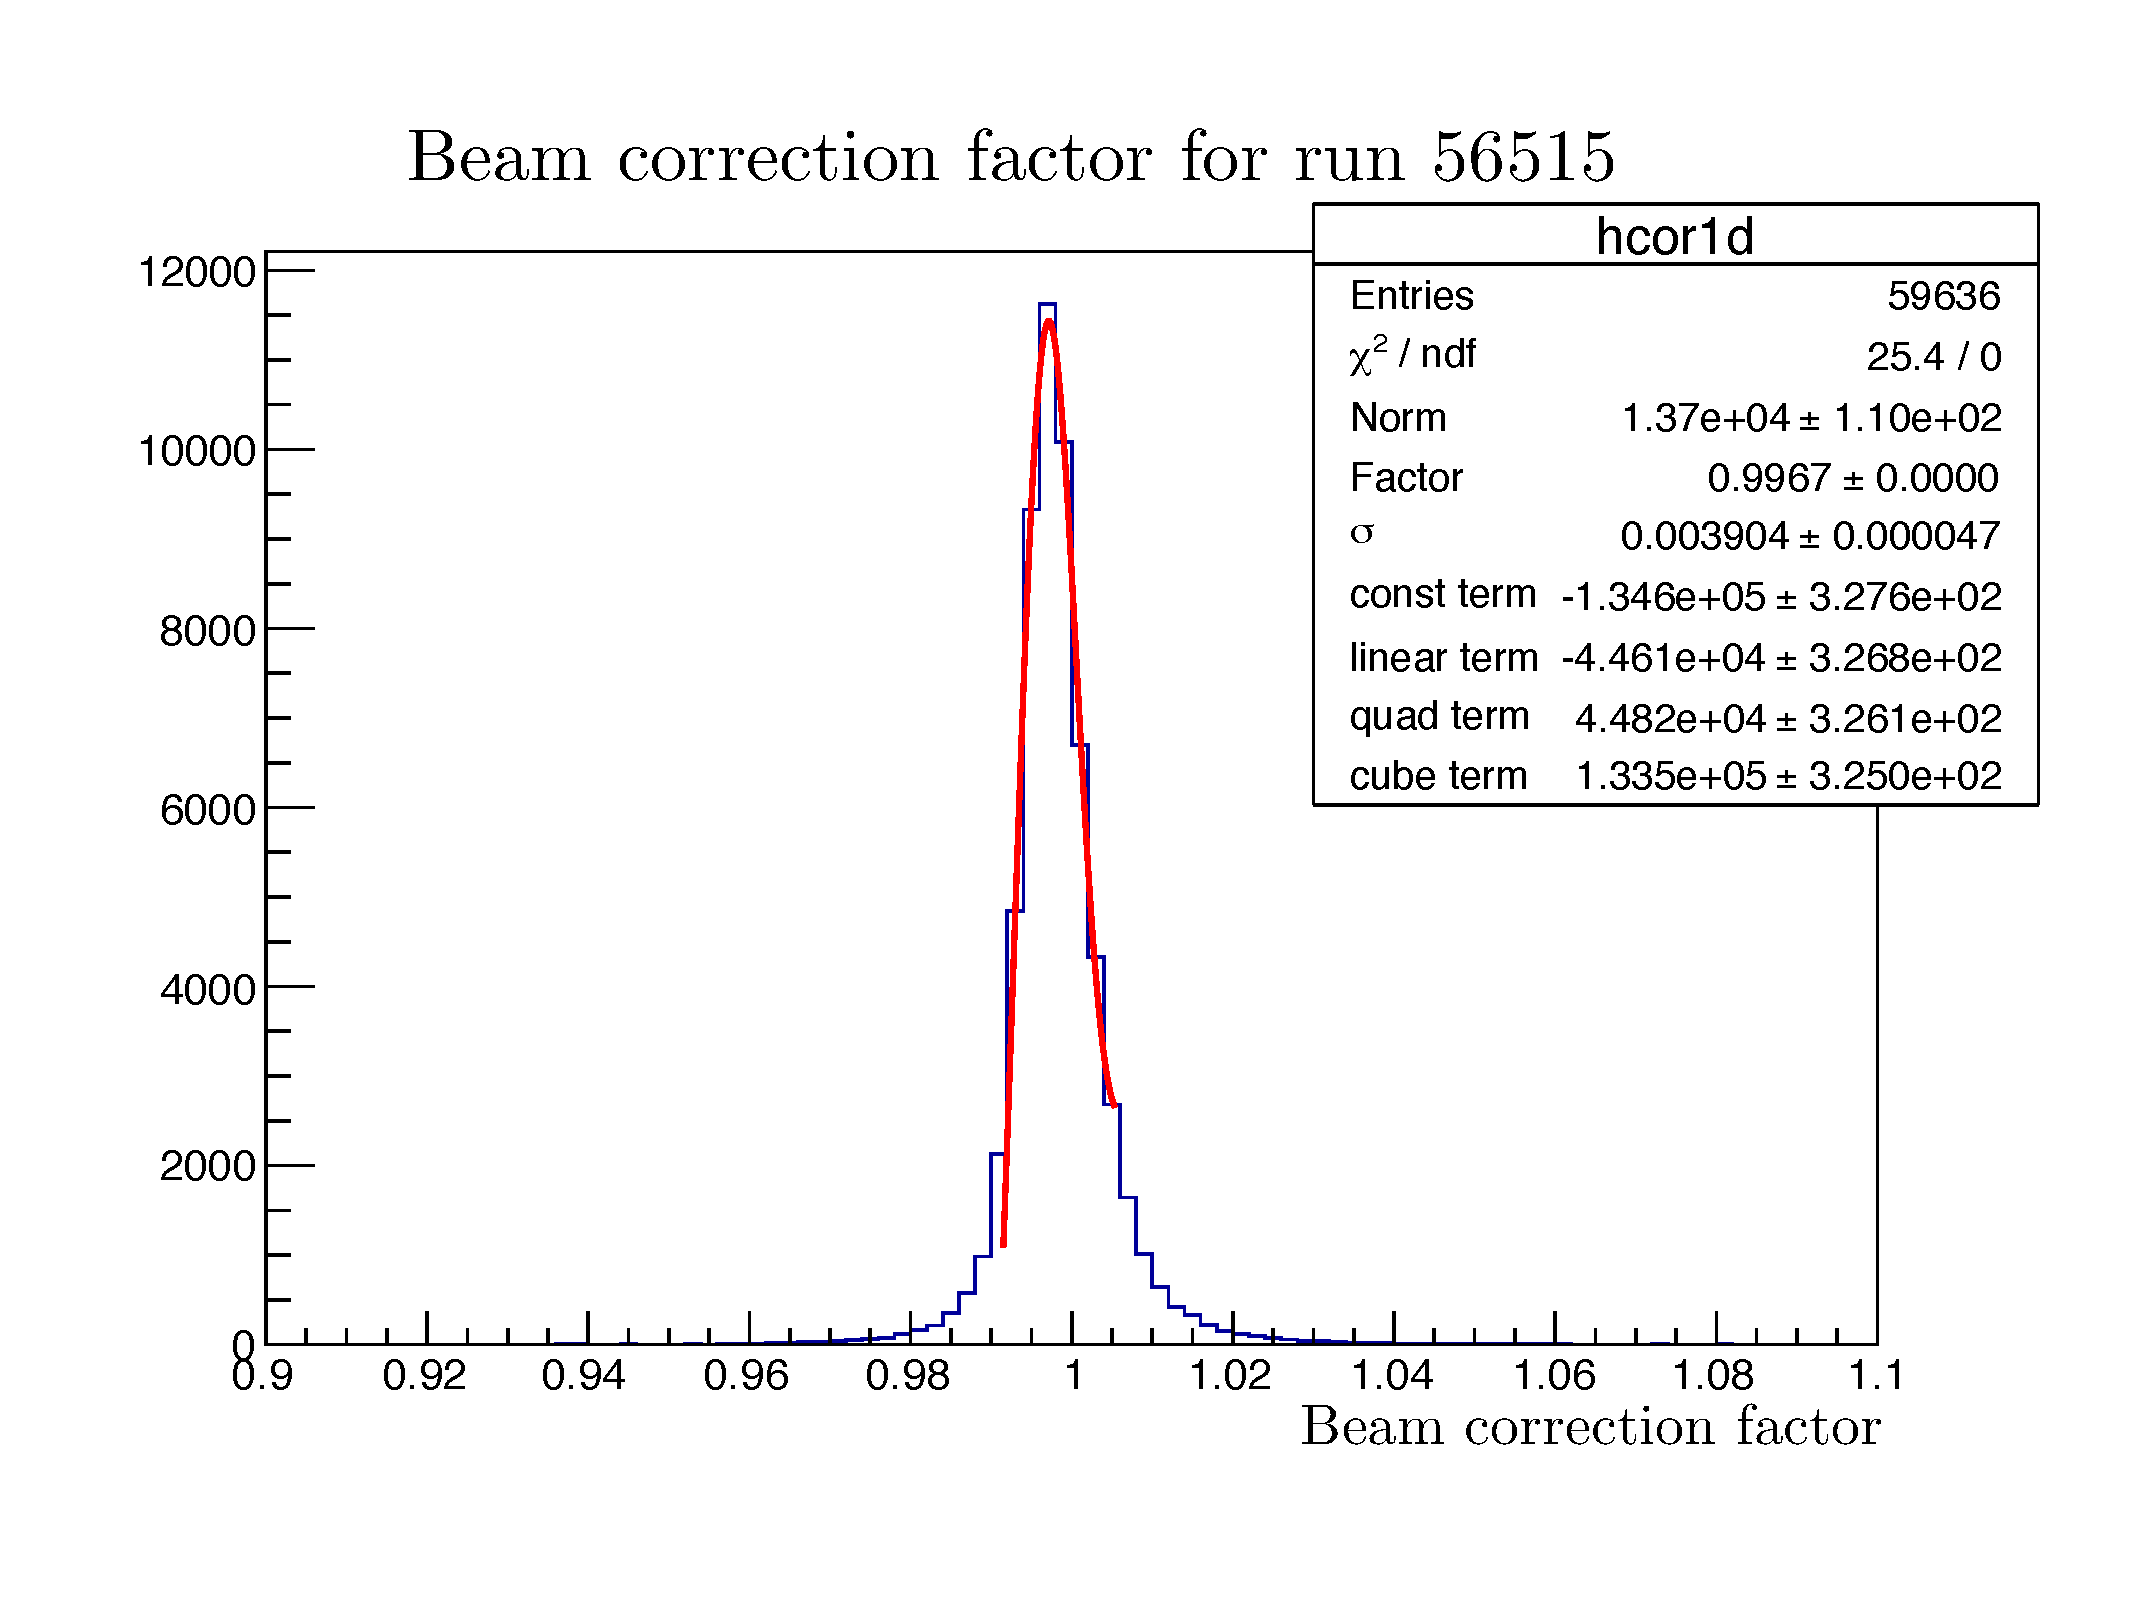
\includegraphics[width=\figwidth,height=0.7\hfigheight]{\figures/analysis/beam_correction/56515_cor.pdf}
  \caption[Beam correction factor for run 56515]{\label{fig:56515.cor} Beam correction factor for run 56515. The fit is a Gaussian function.}
    \end{center}\end{figure}
    
    \begin{figure}[h!]\begin{center}
    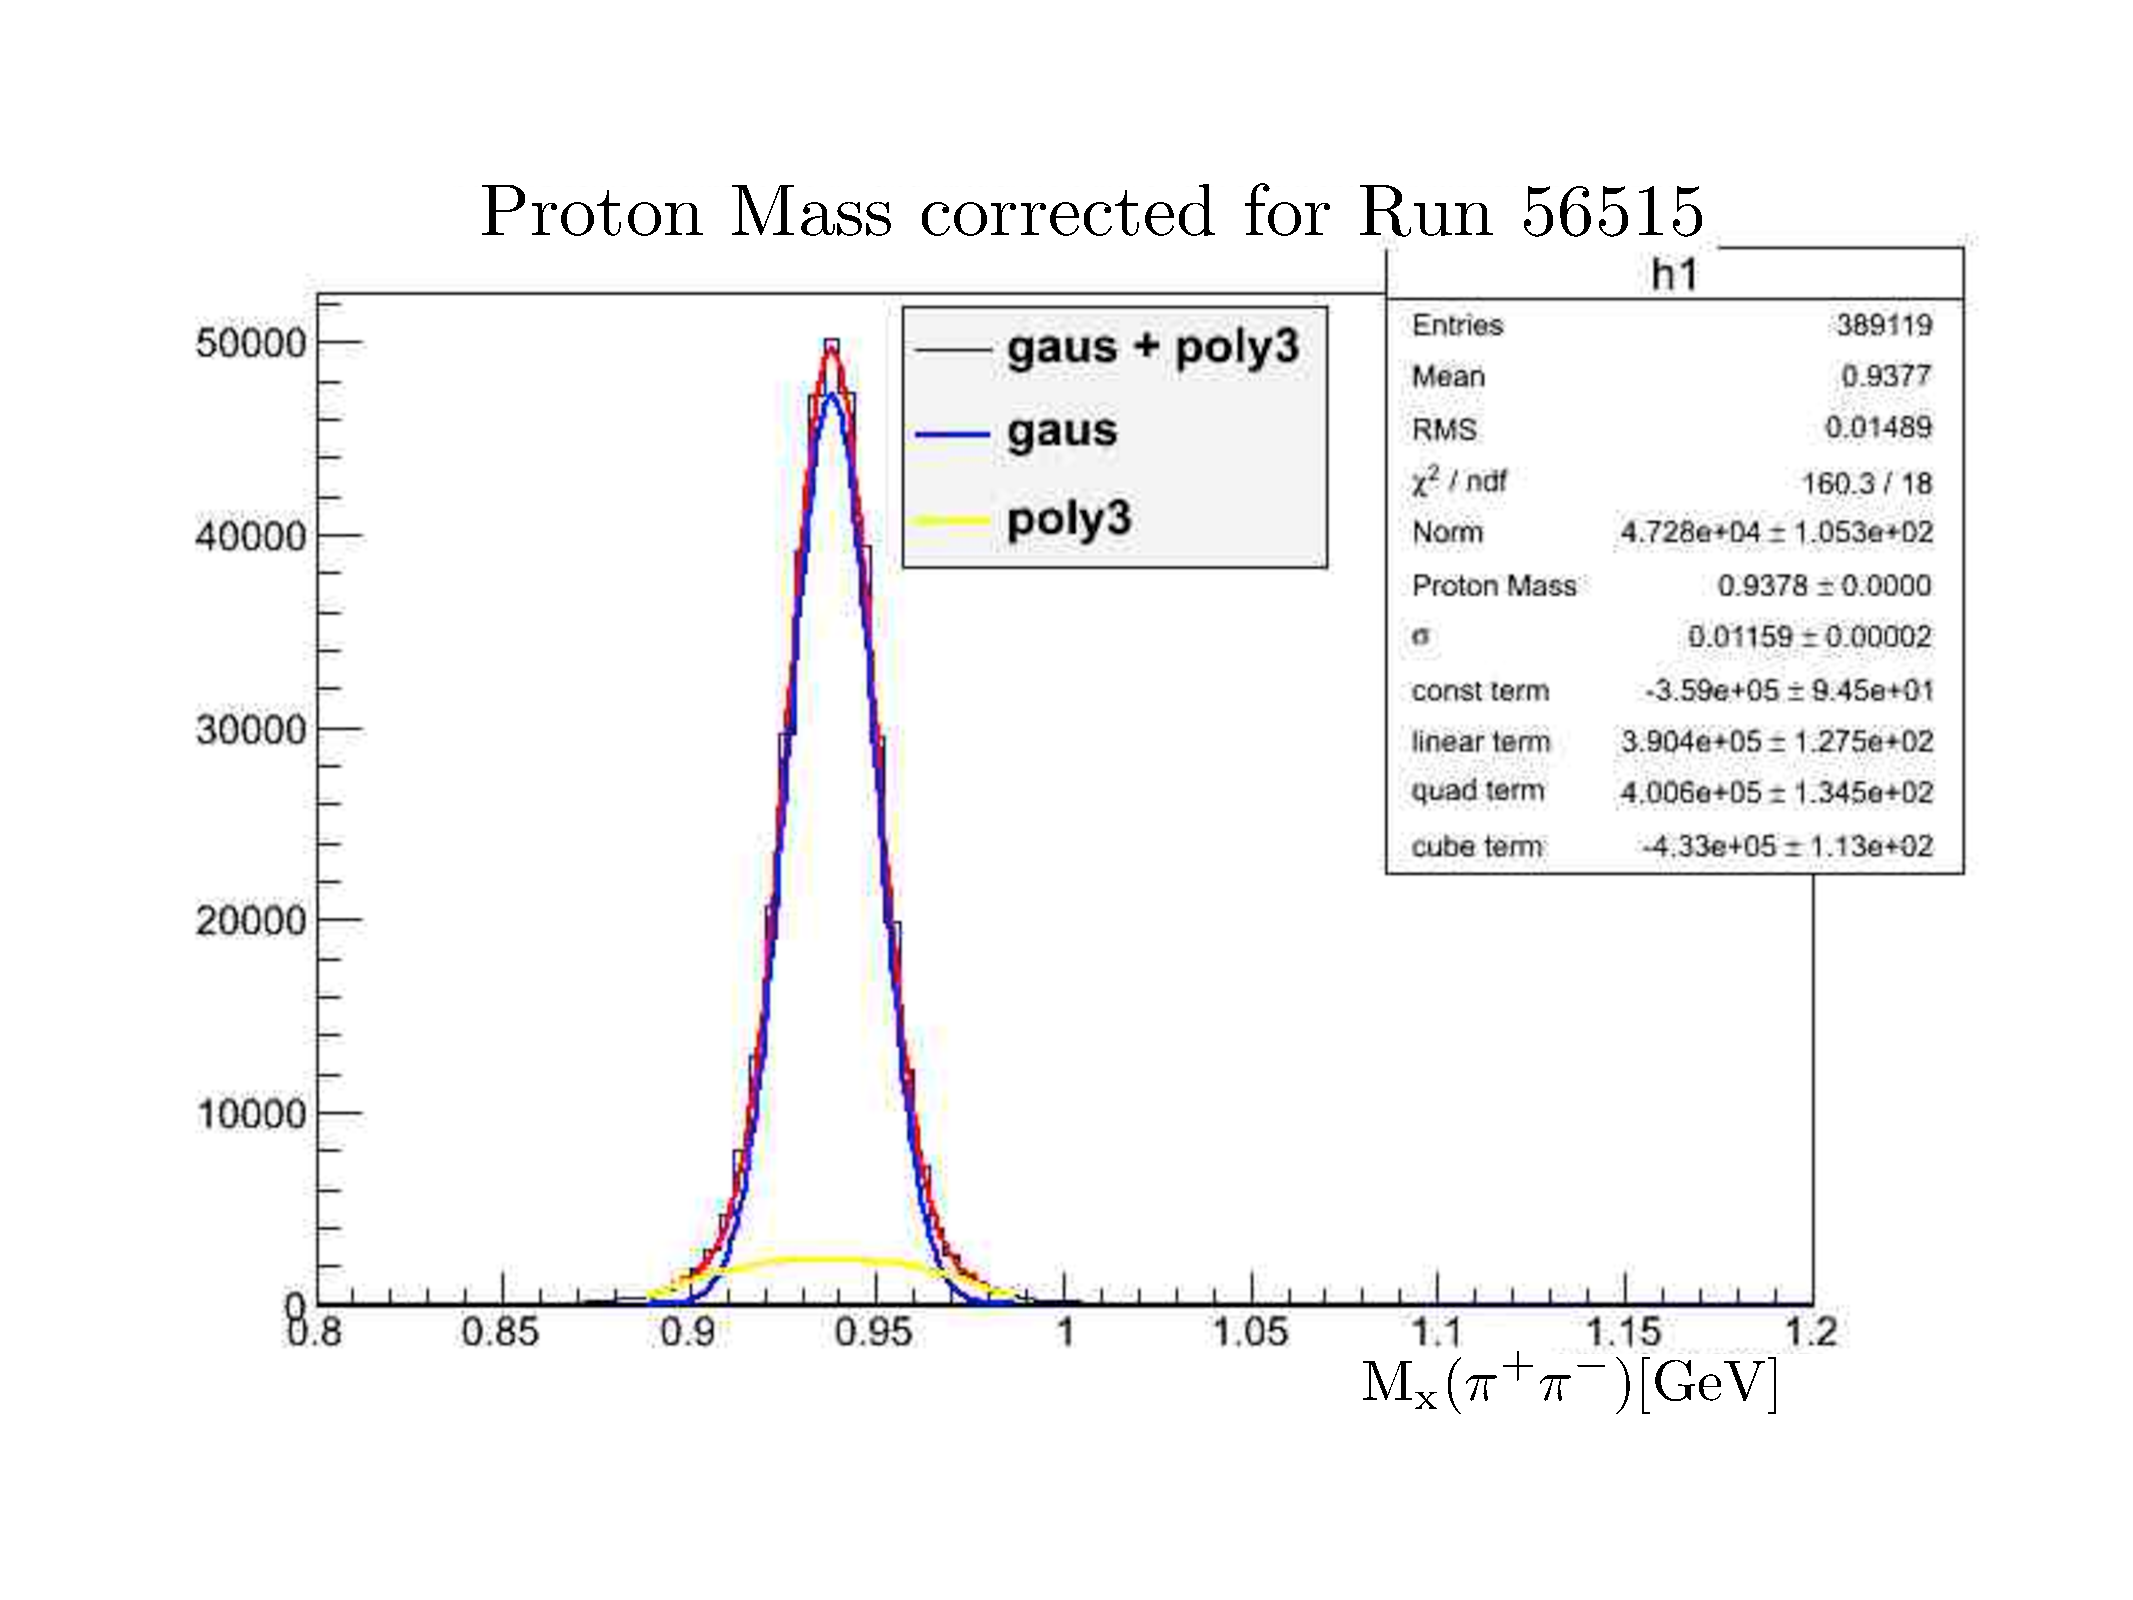
\includegraphics[width=\figwidth,height=0.7\hfigheight]{\figures/analysis/beam_correction/FixedmisssingmassII.pdf}
    \caption[Plot of proton mass for runs 56515 after beam correction was applied]{\label{fig:proton.fix} Plot of proton mass for runs 56515 after beam correction was applied.  \abbr{PDG} mass for the proton is 0.938272 GeV/c.}
    \end{center}\end{figure}
    
    \begin{figure}[h!]\begin{center}
    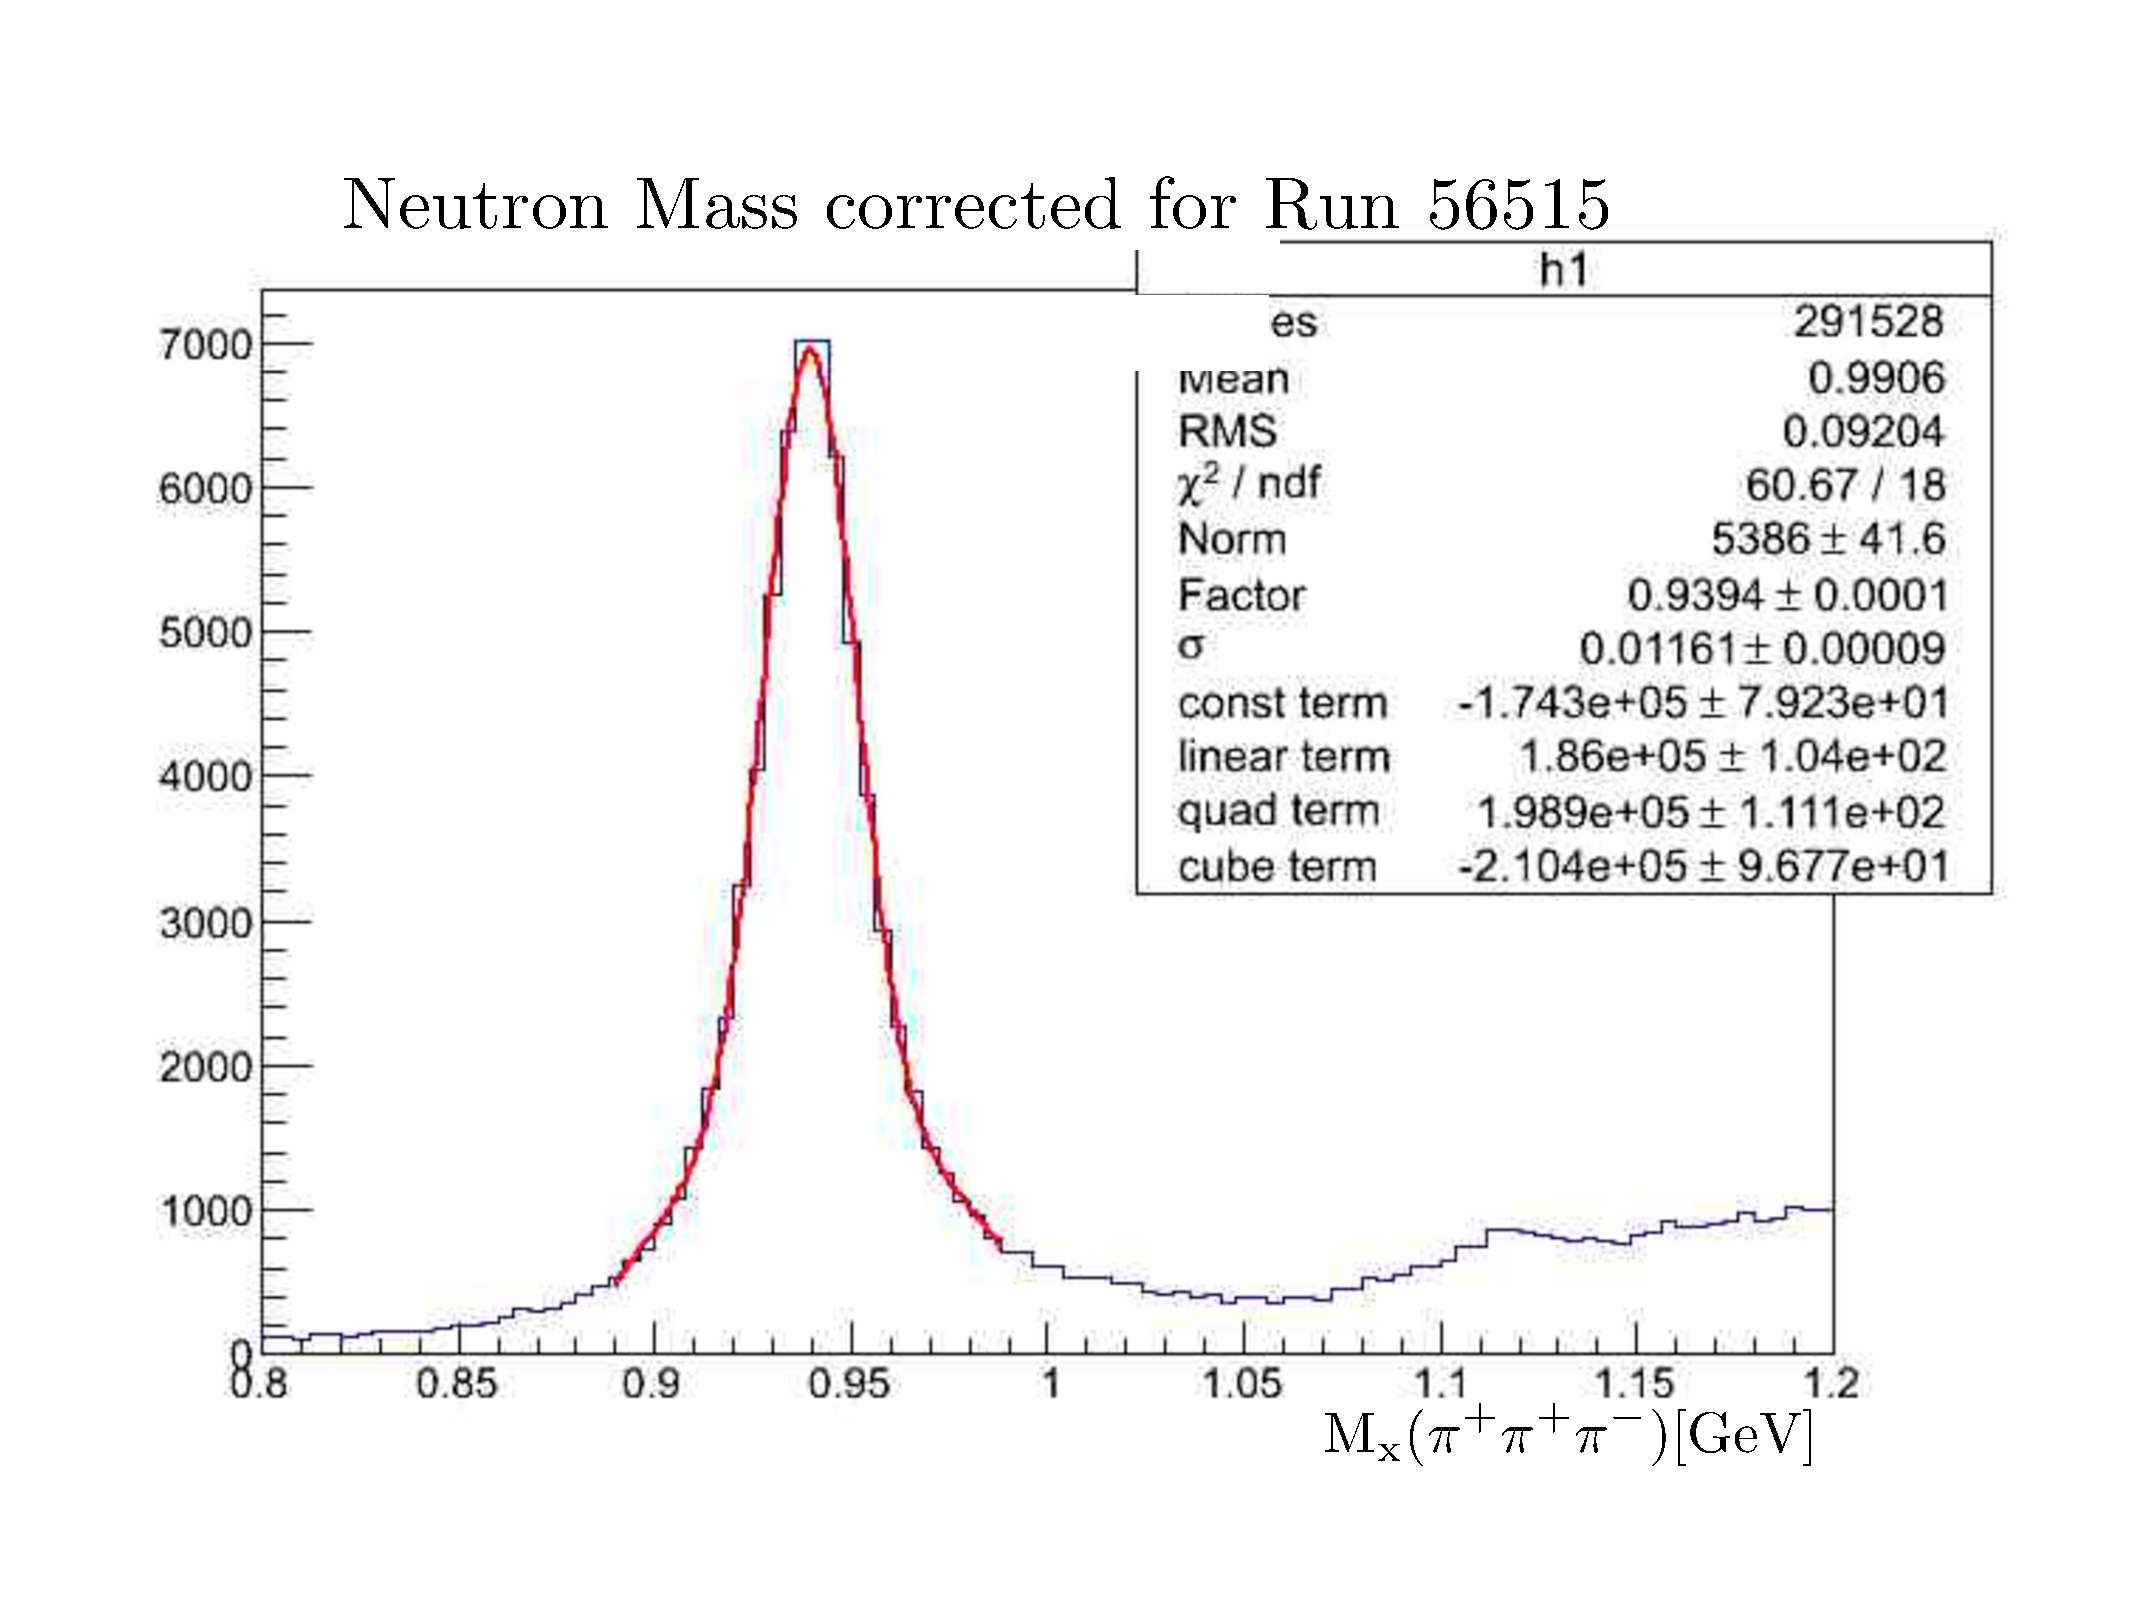
\includegraphics[width=\figwidth,height=0.7\hfigheight]{\figures/analysis/beam_correction/FixedmisssingmassneutronII.pdf}
    \caption[Plot of neutron mass for runs 56515 after beam correction was applied]{\label{fig:neutron.fix} Plot of neutron mass for runs 56515 after beam correction was applied.  \abbr{PDG} mass for the neutron is 0.939565 GeV/c.}
    \end{center}\end{figure}
    
    \begin{figure}[h!]\begin{center}
    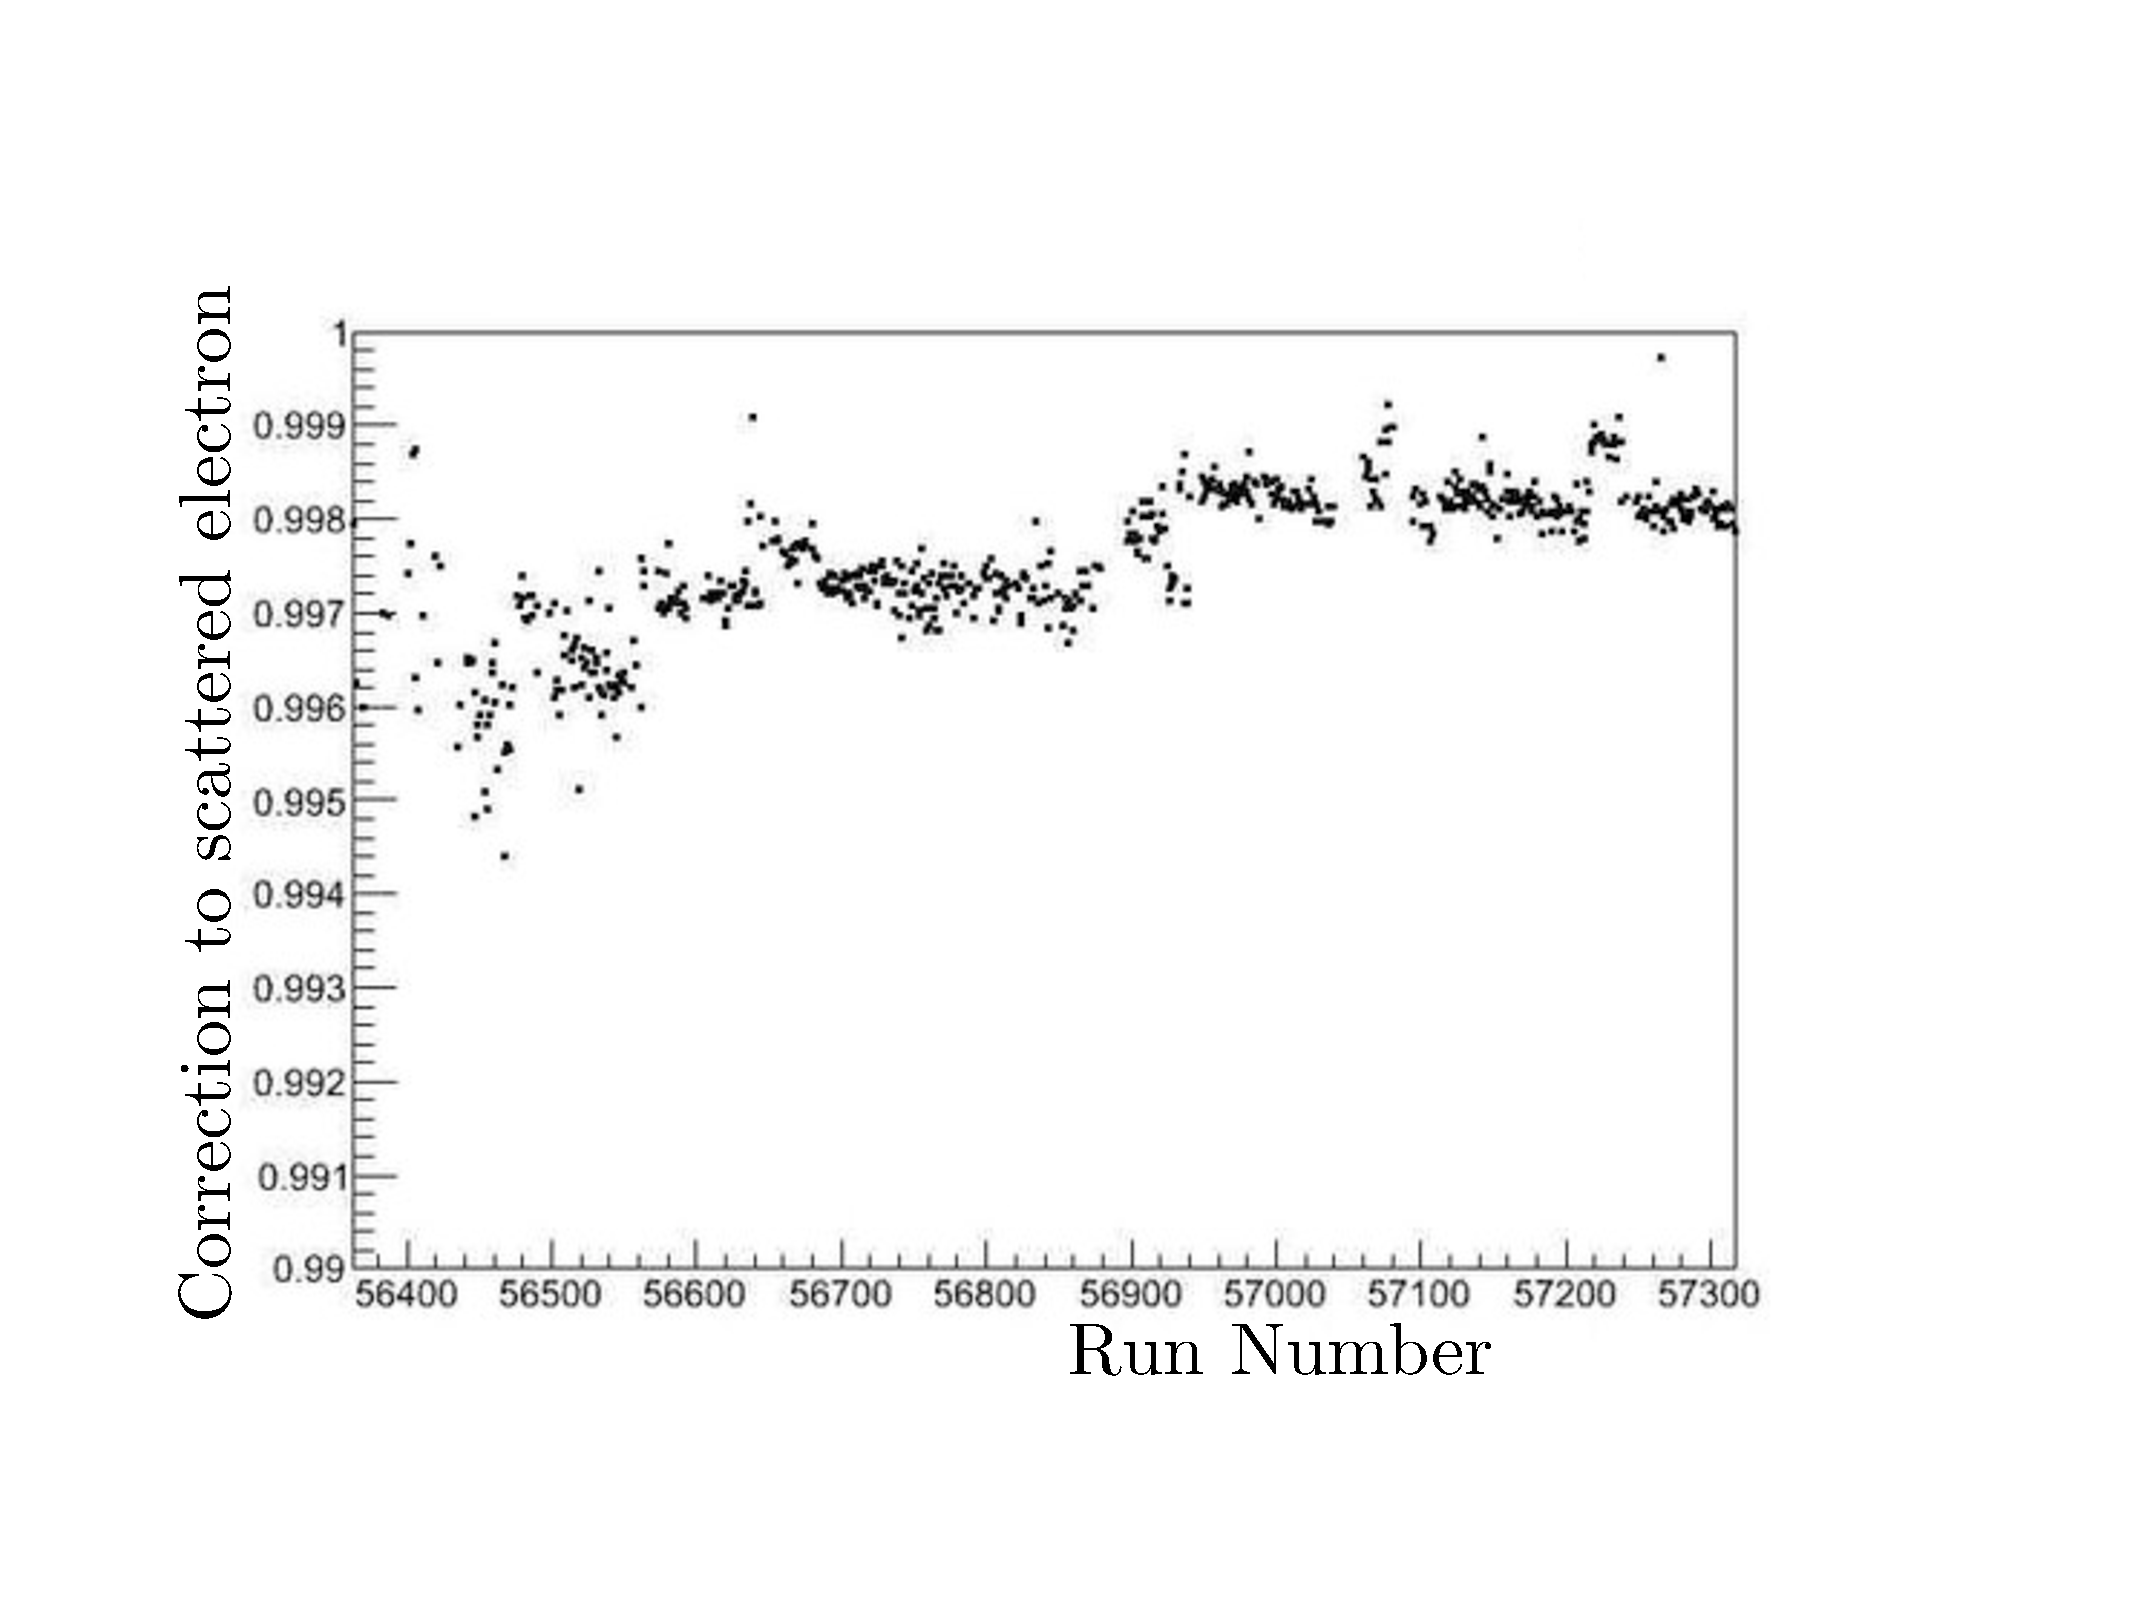
\includegraphics[width=\figwidth,height=0.7\hfigheight]{\figures/analysis/beam_correction/beam_cor.pdf}
    \caption[Plot of the correction factor $x$ as a function of run number]{\label{fig:beamcor.run} Plot of the correction factor $x$ as a function of run number.}
    \end{center}\end{figure}
    
    \begin{figure}[h!]\begin{center}
    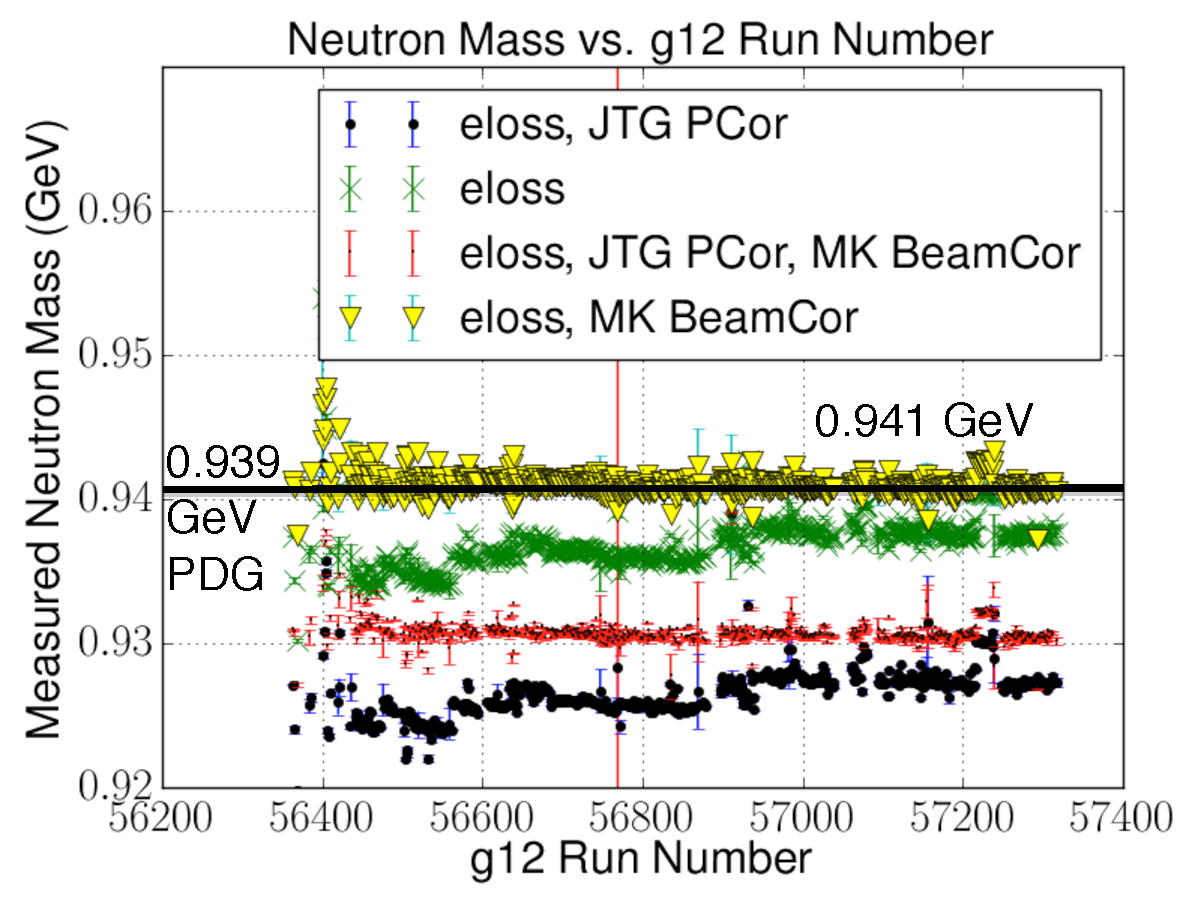
\includegraphics[width=\figwidth,height=0.7\hfigheight]{\figures/analysis/beam_correction/C3pi_allcorr_neutron_rxr.pdf}
    \caption[Plot of missing neutron mass vs. run number using various corrections]{\label{fig:neutron.fixall} Plot of missing neutron mass vs. run number using various corrections. The yellow triangles show a missing neutron mass with only ``energy-loss'' and beam correction applied (MK BeamCor) which was the only corrections needed to correct the \g12 data stream.}
    \end{center}\end{figure}
    
    %
    % Arne Freyberger
    
    \FloatBarrier

\section{Fiducial Cuts}\label{sec:analysis.data.reduction}
This section will describe the various detector performance cuts that were used in this analysis to clean the data due to various subsystems deficiencies. These deficiencies are not understood well enough to be modeled in the \abbr{MC}, therefore some events must be removed from the analysis. 
\subsection{Geometric Fiducial Cuts}\label{sec:analysis.fid_cuts}

 A fiducial cut is required to prevent a significant systematic error contribution from either gaining or loosing events that lie in nonuniform regions, such as space between sectors. This cut, shown in Figs.~\ref{fig:pos:fidcut_all},~\ref{fig:neg:fidcut_all}, was applied to all data, real and simulated, presented in the final result shown in Sec.~\ref{sec:results}. The geometric fiducial cuts analysis was performed by Jason Bono of the FIU group. The package for performing these fiducial cuts has three options for the parameters involved in the removal process. These options are ``loose", ``nominal" and ``tight" and refer to the amount of area that is to be cut in the space between the drift chambers. A detailed specification of this cut is given in~\cite{clas.g12.note}. This analysis used the nominal option. To understand the systematic error caused in this fiducial, the measurement from the ``tight" option was compared to the measurement at the nominal option. This is discussed in Sec.~\ref{sec:results.systematics}.

\begin{figure}[h!]\begin{center}
\subfloat[Positive Charge Particle Before Geometric Fiducial Cut][]{ %Feynman diagram of \piz two photon decay
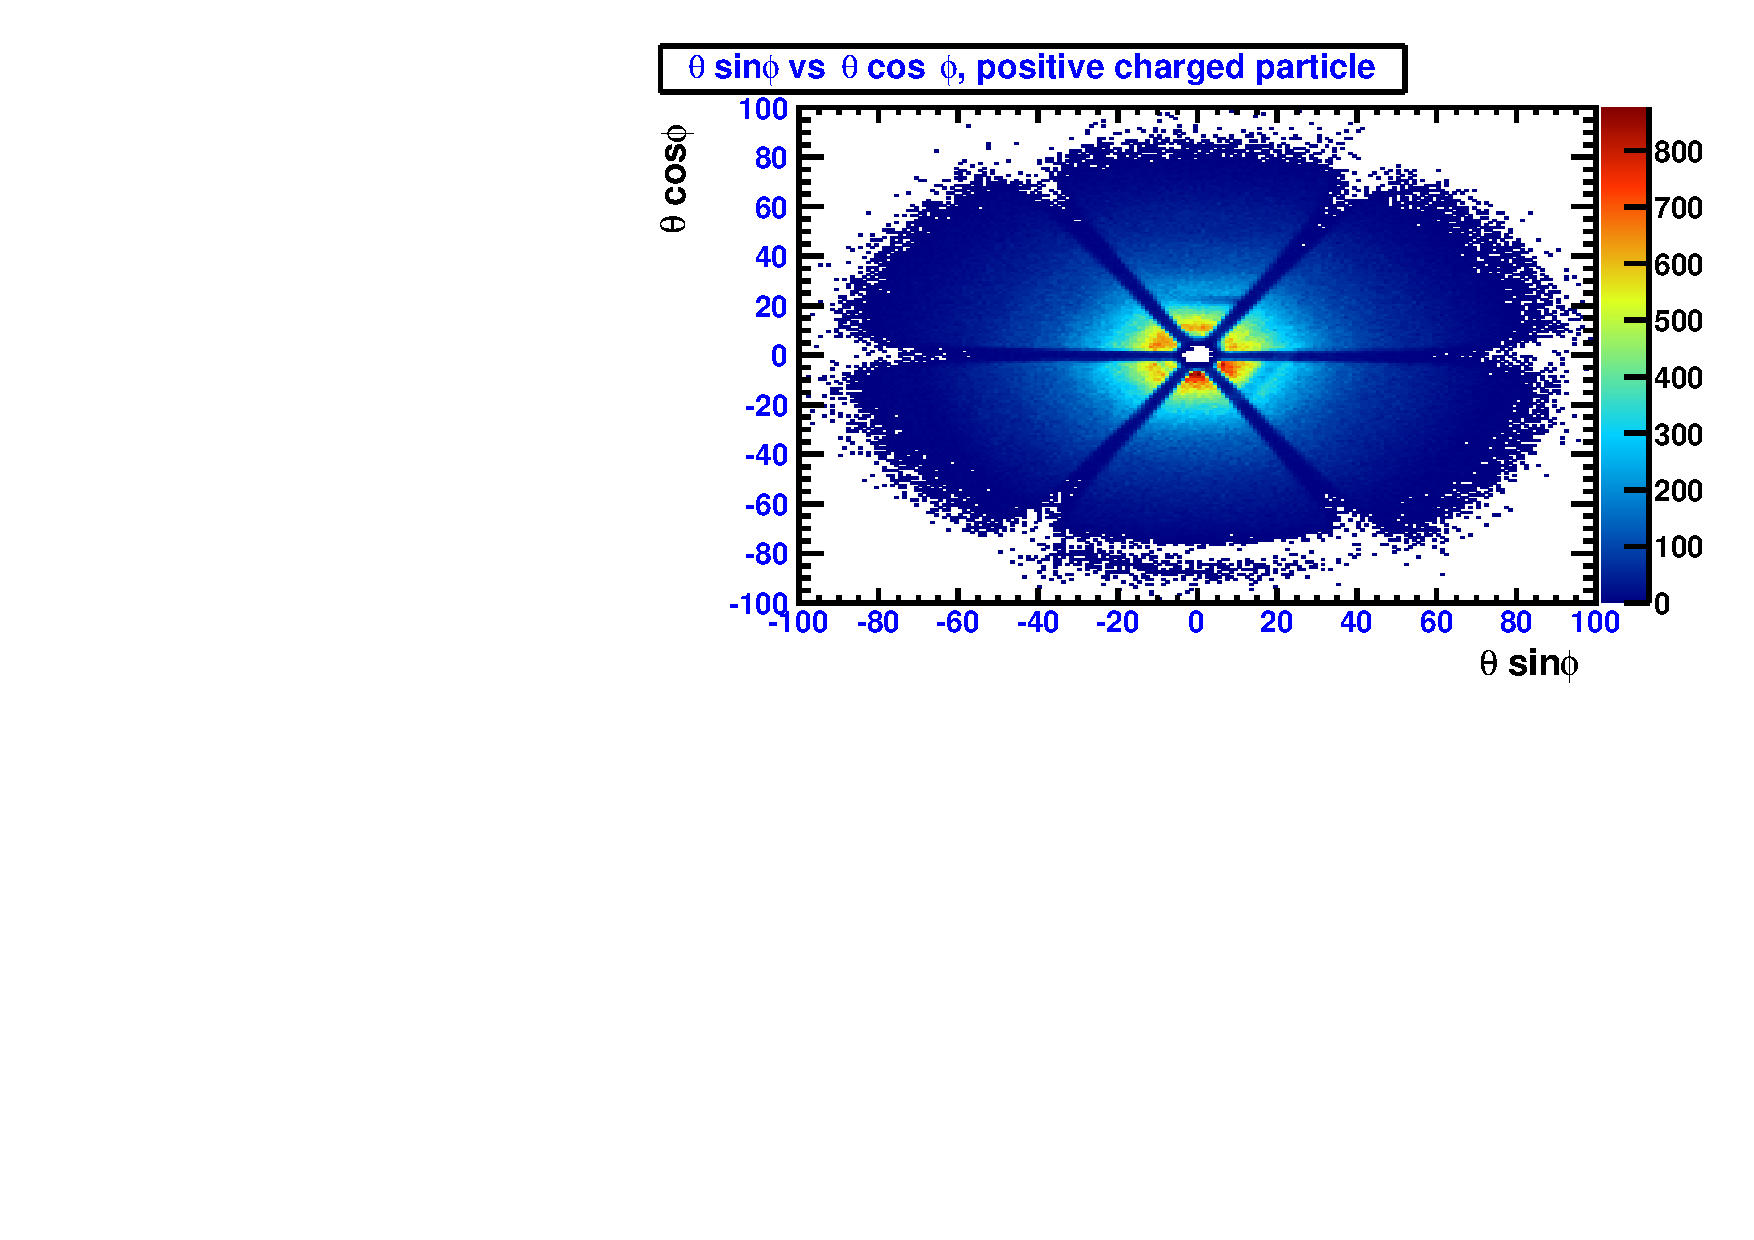
\includegraphics[width=\figwidth,height=\qfigheight]{\grpath/analysis/FIDUCIAL_CUTS/GEOMETRIC/pip_theta_cos_sin_phi_nofid.pdf}\label{fig:pos:fidcut_off}
}\\
\subfloat[Positive Charge Particle After Geometric Fiducial Cut][]{ %Feynman diagram of \piz Dalitz decay
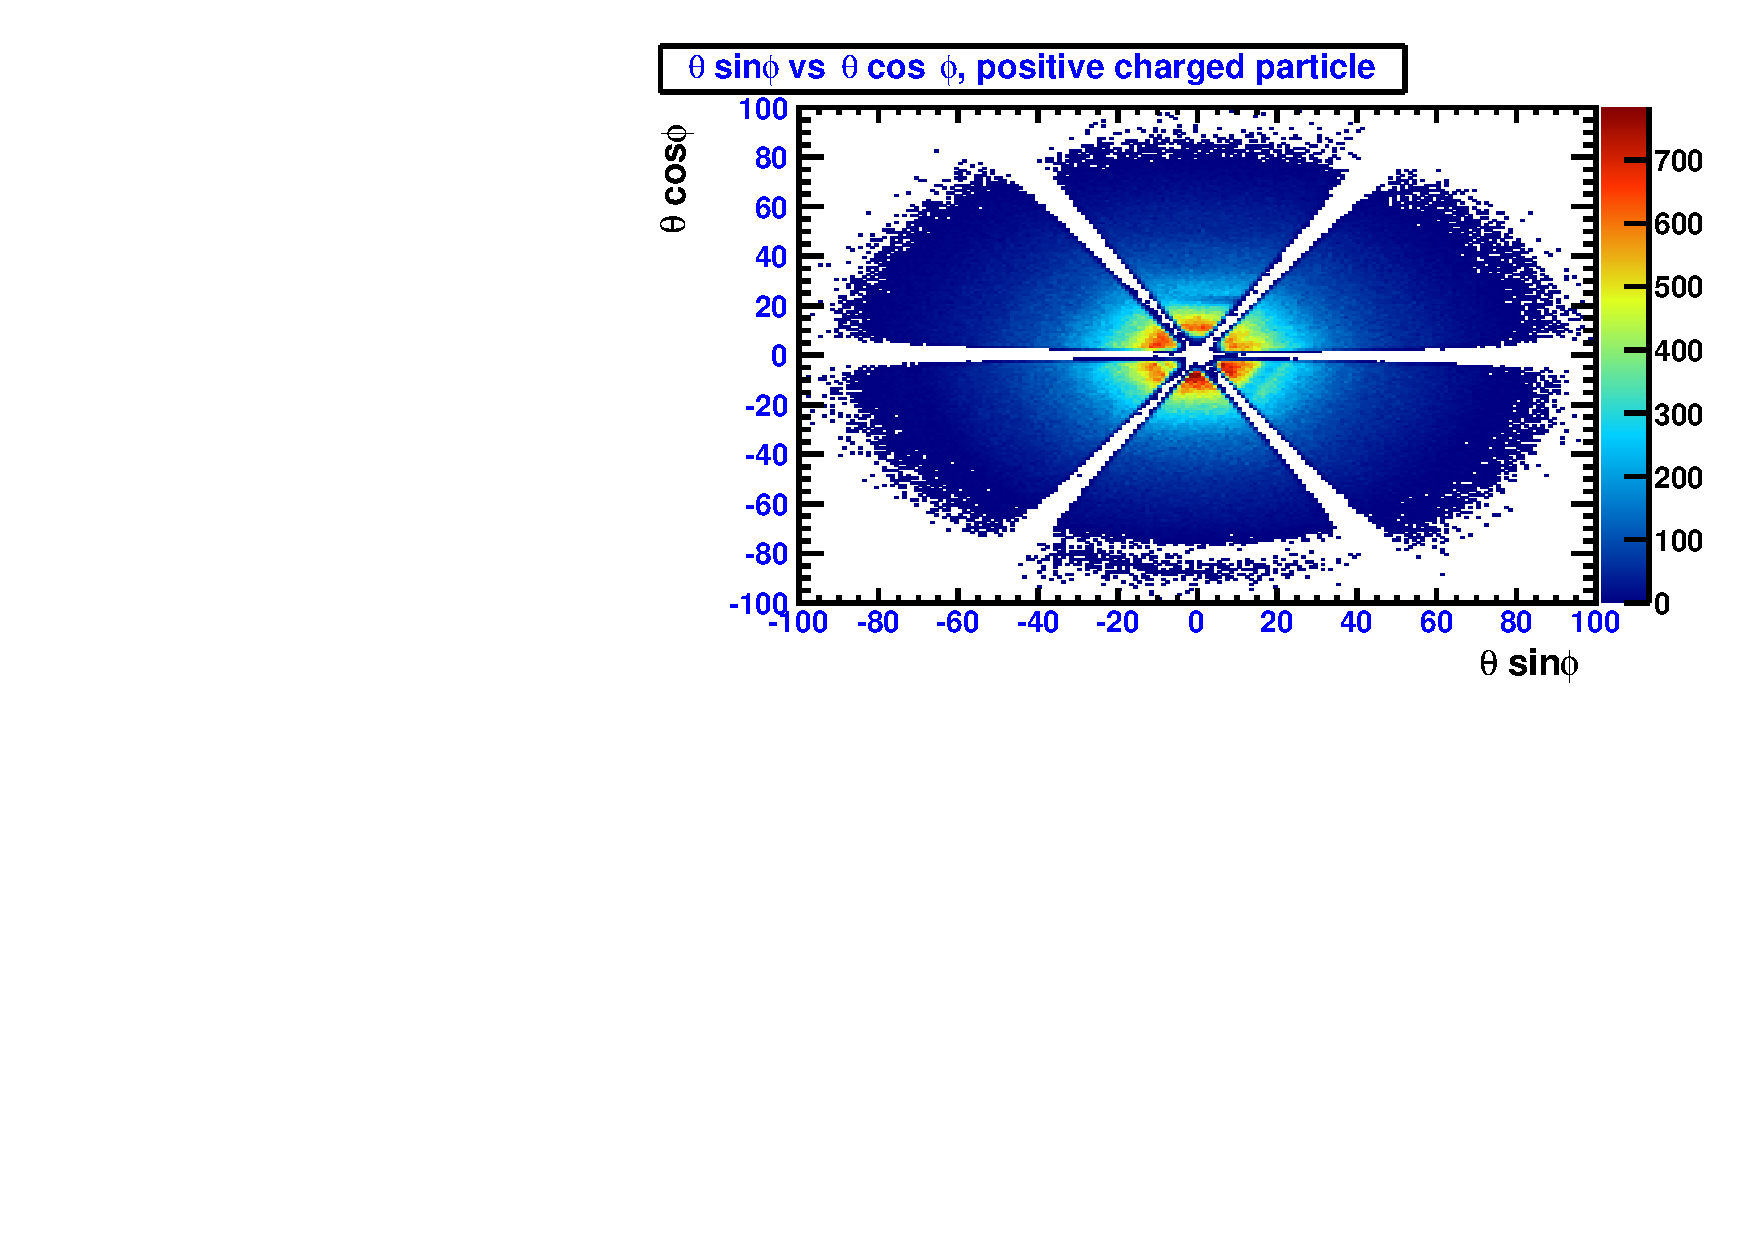
\includegraphics[width=\figwidth,height=\qfigheight]{\grpath/analysis/FIDUCIAL_CUTS/GEOMETRIC/pip_theta_cos_sin_phi_wfid.pdf}\label{fig:pos:fidcut_on}
}
\caption[Positive charged tracks in \abbr{CLAS} \abbr{DC} prior to fiducial cuts being applied, and after being applied]{\label{fig:pos:fidcut_all}Positive charged tracks in \abbr{CLAS} \abbr{DC} prior to fiducial cuts~\subref{fig:pos:fidcut_off} being applied, and after~\subref{fig:pos:fidcut_on} being applied.}

\end{center}\end{figure}
%
\begin{figure}[h!]\begin{center}
\subfloat[Negative Charge Particle Before Geometric Fiducial Cut][]{ %Feynman diagram of \piz two photon decay
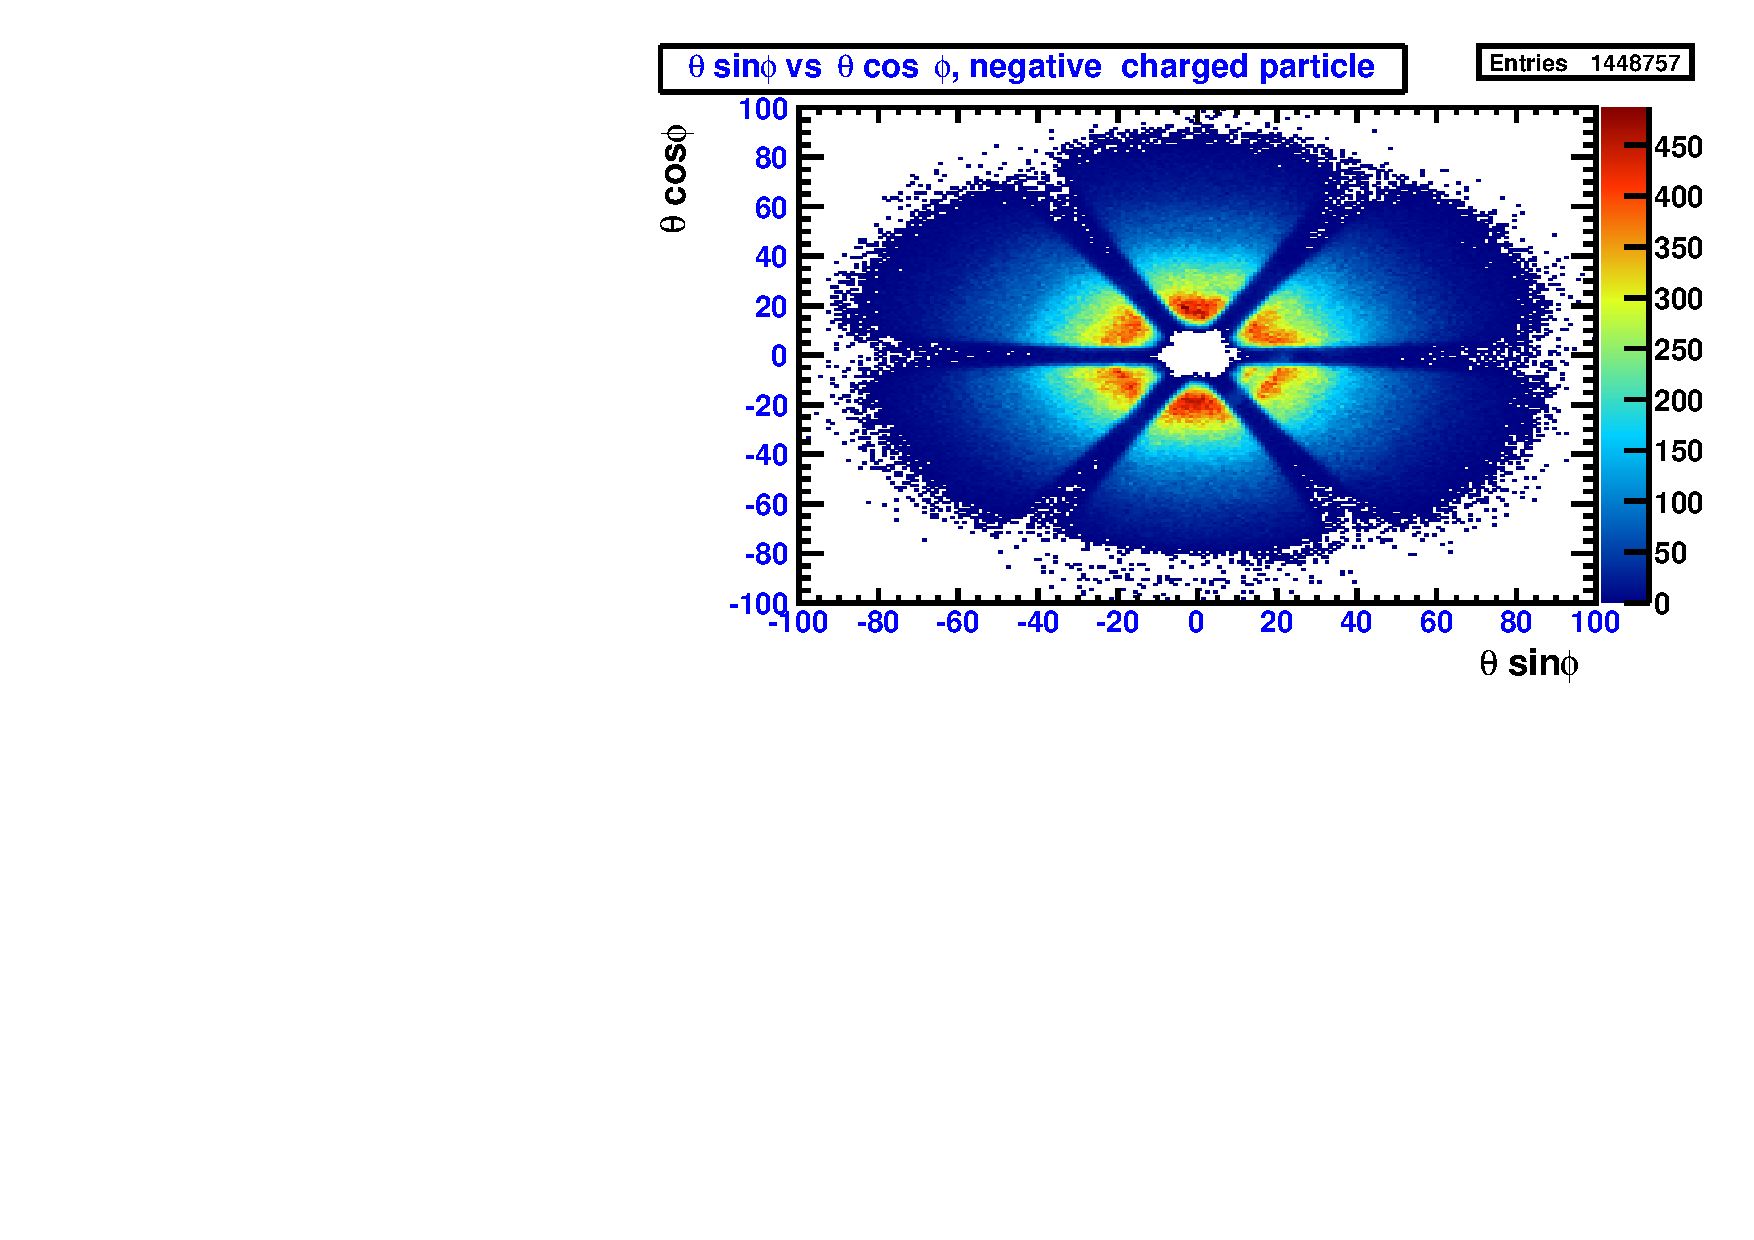
\includegraphics[width=\figwidth,height=\qfigheight]{\grpath/analysis/FIDUCIAL_CUTS/GEOMETRIC/pim_theta_cos_sin_phi_nofid.pdf}\label{fig:neg:fidcut_off}
}\\
\subfloat[Negative Charge Particle After Geometric Fiducial Cut][]{ %Feynman diagram of \piz Dalitz decay
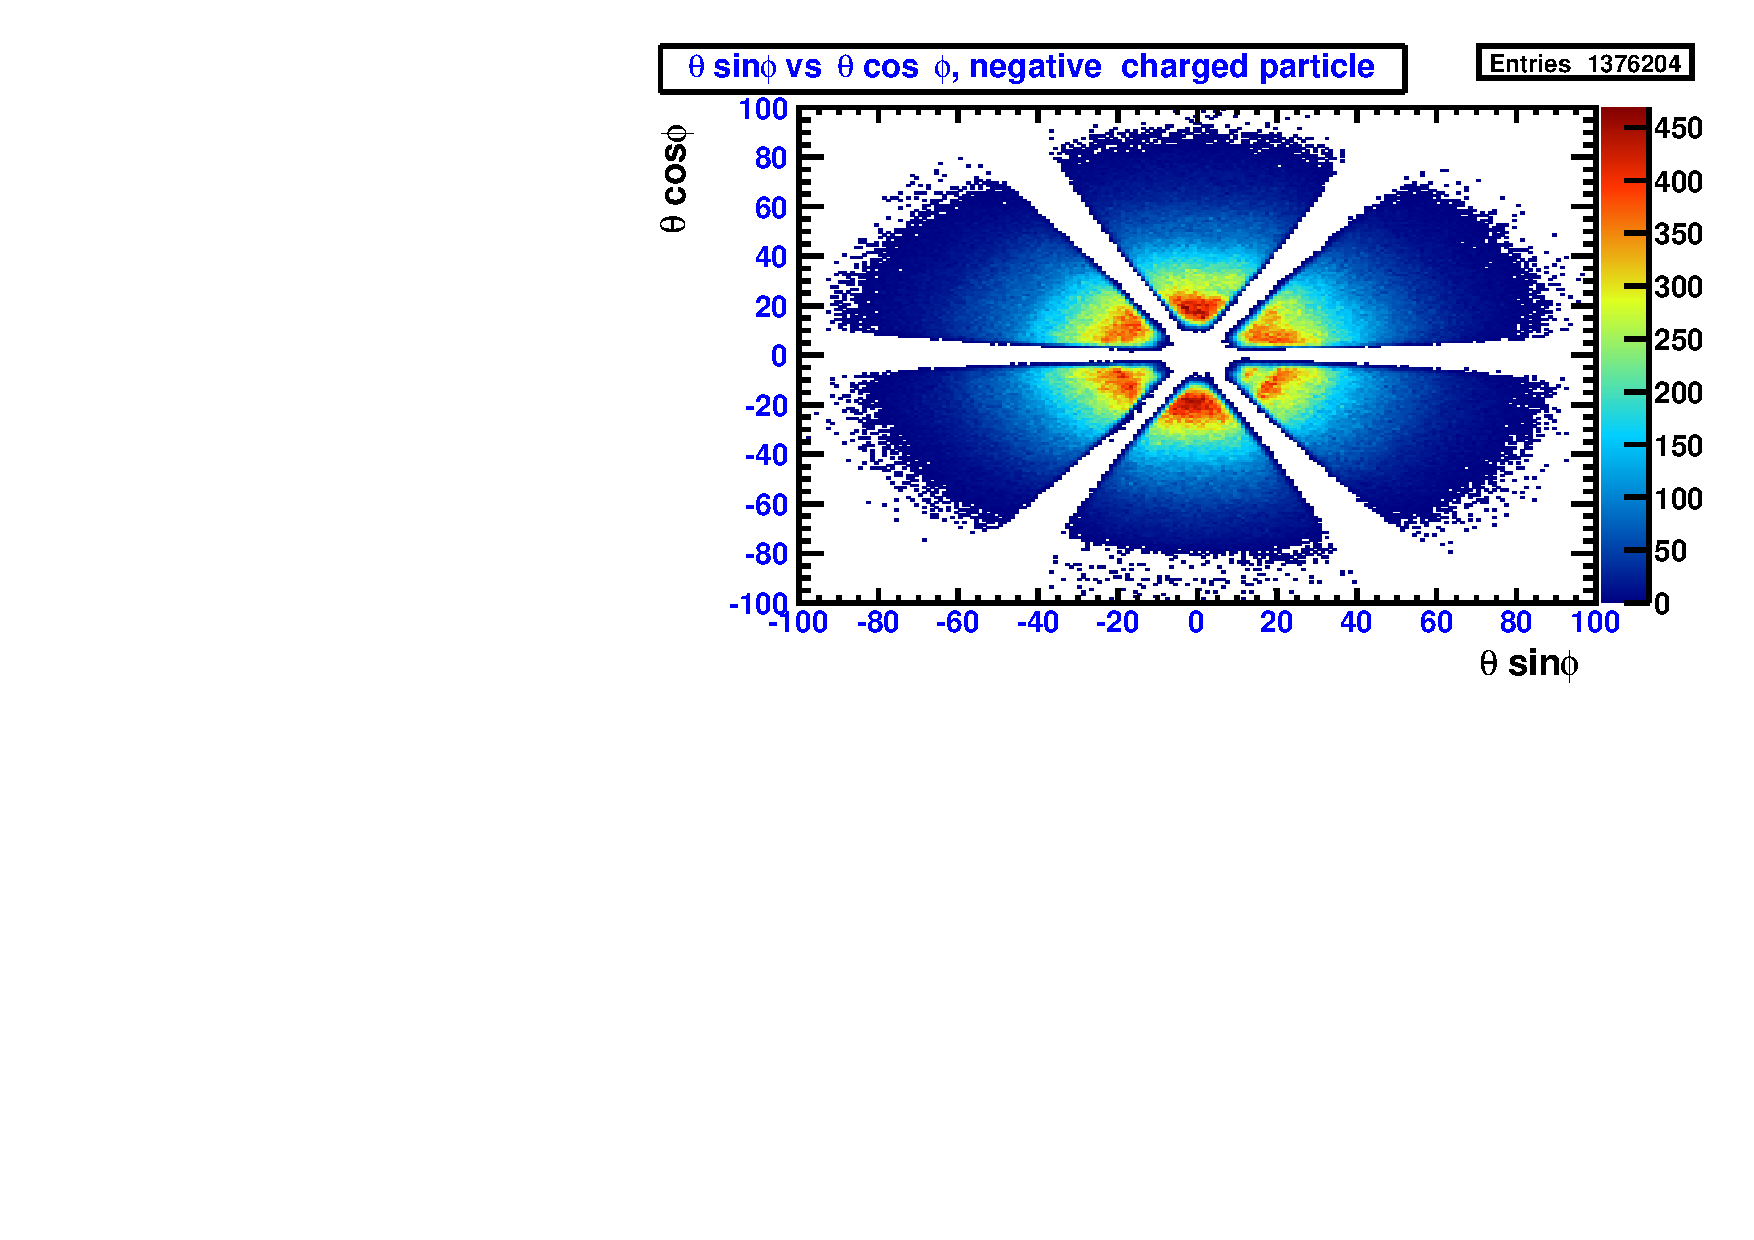
\includegraphics[width=\figwidth,height=\qfigheight]{\grpath/analysis/FIDUCIAL_CUTS/GEOMETRIC/pim_theta_cos_sin_phi_wfid.pdf}\label{fig:neg:fidcut_on}
}
\caption[Negative charged tracks in \abbr{CLAS} \abbr{DC} prior to fiducial cuts being applied, and after being applied]{\label{fig:neg:fidcut_all}Negative charged tracks in \abbr{CLAS} \abbr{DC} prior to fiducial cuts~\subref{fig:pos:fidcut_off} being applied, and after~\subref{fig:pos:fidcut_on} being applied.}

\end{center}\end{figure}

\FloatBarrier

\subsection{\abbr{TOF} Fiducial Cuts}\label{sec:analysis.tof_fid}

The efficiency for the \abbr{TOF} subsystem, described in Sec.~\ref{sec:clas.tof}, is different for each paddle for each section. As a result, there are regions of detection in which are inefficient. The program \abbr{GPP}, Sec.~\ref{sec:analysis.simulation}, was constructed to account for these inefficiencies in the simulation. However the \abbr{MC} indicated a greater efficiency than we measured in the data. Therefore we measured the efficiency of \abbr{CLAS} as a function of particle angle and momentum. The particles $\pi^+$, $\pi^-$ and proton momentum and angular measurements were selected from data and \abbr{MC} to analyze these functions. When an inefficiency was observed in the data, but not the \abbr{MC}, equations were derived in $\theta$ and $\phi$ to use as a cut to account for the inefficiency. Example of such an inefficiency can be seen in Fig~\ref{fig:pos:tofcut_off}, where the top panel depicts the $\pi^+$ azimuthal angle~($\phi$) vs. polar angle~($\theta$) and the bottom panel illustrates momentum~($p$) vs. polar angle~($\theta$) for sector 3.
%\begin{table}[h!]
\begin{minipage}{\textwidth}
\begin{center}
\begin{singlespacing}

\caption[Angular Range for \abbr{TOF} Plots]{\label{tab:tof.pipsec3} Angular range for \abbr{TOF} plots}
\begin{tabular}{c|c|c}
\hline												
$\phi$ Range [$\circ$]	& $\theta$ Range [$\circ$] & Plot Panel \\ \hline 	
$90 < \phi < 120$ & $10 < \theta < 45$ & Top Left \\
$90 < \phi < 120$ & $40 < \theta < 90$ & Top Right \\
$120 < \phi < 150$ & $10 < \theta < 45$ & Middle Left \\
$120 < \phi < 150$ & $40 < \theta < 90$ & Middle Right \\
\hline												
Momentum Range [GeV]	& $\theta$ Range [$\circ$] & Plot Panel \\ \hline 
$0 < \mathrm{P} < 2$ & $10 < \theta < 90$ & Bottom \\
\hline \hline%inserts single line
\end{tabular}

\end{singlespacing}
\end{center}
\end{minipage}
\end{table}
\vspace{20pt}
%At the time of writing this manuscript, there was no reliable hypothesis for dealing with the \abbr{TOF} at the \abbr{TOF} subsystem level or \abbr{TOF} paddle level.
Fig.~\ref{fig:pos:tofcut_off} shows a band of low efficiency pertaining to a inefficient \abbr{TOF} paddle between$\approx 15^\circ < \theta < 21^\circ$. Fig.~\ref{fig:pos:tofcut_off} also shows a ``rib" like structure on the bottom plot, $\theta$ vs. $p$, which is not present in the $\pi^-$ data, therefore was not further investigated as a bad paddle. The inefficient section of sector 3 was removed in data and \abbr{MC}. The effect of this cut can be seen in Fig.~\ref{fig:pos:tofcut_on}. The statistical sample used in Fig.~\ref{fig:pos:tofcut_on} was $1/5$ of the data used to derive the cut equation shown in Fig~\ref{fig:pos:tofcut_off}. There also existed an inefficiency in sector 1. The plots showing the inefficiency along with the other 5 sectors can be found in App.~\ref{sec:app.tof_plots}. The parameters for the \abbr{TOF} cuts are listed in Tab.~\ref{tab:tof.eq}. Placing the cuts described in Tab.~\ref{tab:tof.eq} is equivalent to knocking out \abbr{TOF} paddle by ID number. The variable $\phi_s$ is $\phi$ represented in the interval of $-30\le \phi \le30$ in which the term $f_{mod}$ is the $C++$ function used to perform the operation.
\begin{table}[h!]
\begin{minipage}{\textwidth}
\begin{center}
\begin{singlespacing}

\caption[\abbr{TOF} Cut Parameters]{\label{tab:tof.eq} \abbr{TOF} cut parameters.}
\begin{tabular}{c|c|c|c}
\hline												
Sector	& $\phi [^\circ]$ & $\theta$ Upper Limit ($<=$) & $\theta$ Lower Limit ($>=$)  \\ \hline 	
1 & $\phi<0$ &  $24-\phi(26-24)/30$ & $ 21.5-\phi(23.5-21.5)/30$  \\
1 & $\phi>=0$ & $ 24+\phi(26-24)/30$ & $ 21.5+\phi(23.5-21.5)/30$  \\
3 & $\phi_{s}<0$ & $ 20.5-\phi_{s}(22.-20.5)/30$ & $ 16-\phi_{s}(17.5-16)/30$  \\
3 & $\phi_{s}>=0$ & $ 20.5+\phi_{s}(22-20.5)/30$ & $ 16.+\phi_{s}(17.5-16)/30$  \\
\hline
\multicolumn{4}{c}{$\phi_{s} = fmod(fmod((\phi+390),360),60) - 30$} \\
\hline \hline%inserts single line
\end{tabular}

\end{singlespacing}
\end{center}
\end{minipage}
\end{table}
\vspace{20pt}
%Where $\phi_{s} = fmod(fmod((\phi+390),360),60) - 30$.

%1 & $\phi<0$ &  $\theta <= 24.+((26.-24.)/-30.)\phi$ & $\theta >= 21.5+((23.5-21.5)/-30.)\phi$  \\
%1 & $\phi>=0$ & $ \theta <= 24.+((26.-24.)/30.)\phi$ & $\theta >= 21.5+((23.5-21.5)/30.)\phi$  \\
%3 & $\phi_{s}<0$ & $\theta <= 20.5+((22.-20.5)/-30.)\phi_{s}$ & $\theta >= 16.+((17.5-16.)/-30.)\phi_{s}$  \\
%3 & $\phi_{s}>=0$ & $\theta <= 20.5+((22.-20.5)/30.)\phi_{s}$ & $\theta >= 16.+((17.5-16.)/30.)\phi_{s}$  \\  
%Where $\phi_{s} = fmod(fmod((\phi+390),360),60) - 30$.


\begin{figure}[h!]\begin{center}
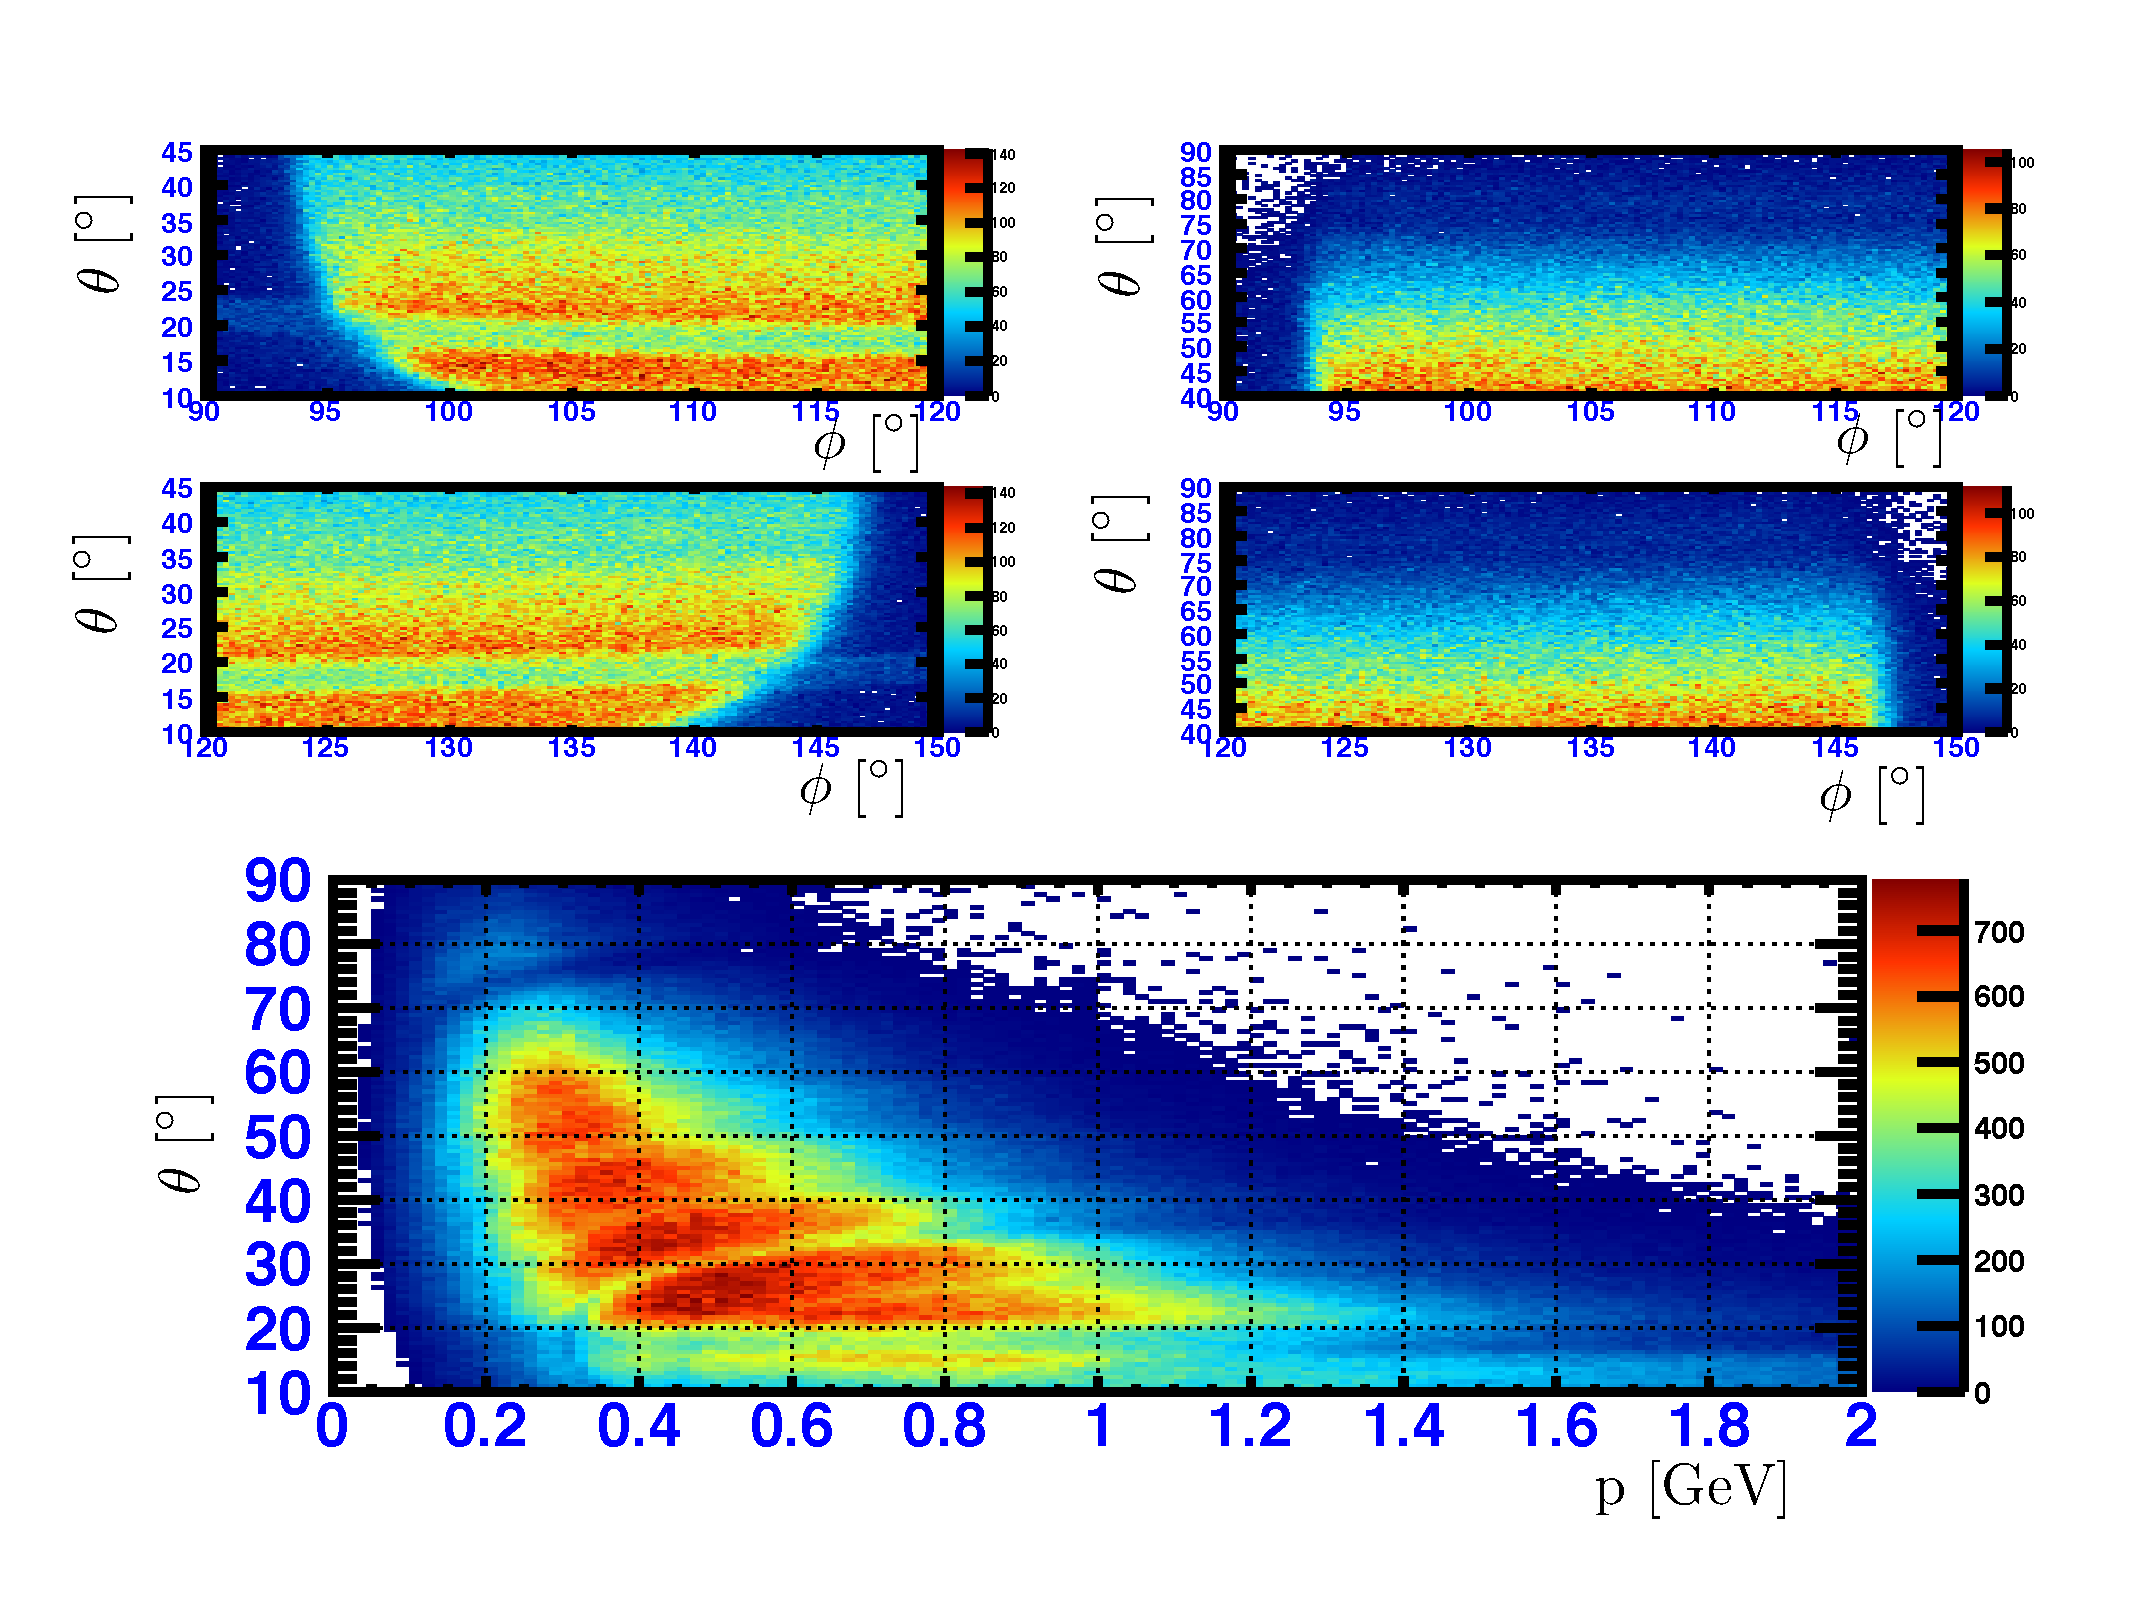
\includegraphics[width=\figwidth,height=\hfigheight]{\grpath/analysis/FIDUCIAL_CUTS/TOF/RAW/pip_sec3.pdf}
\caption[$\theta$ vs. $\phi$ of $\pi^+$ data]{\label{fig:pos:tofcut_off}(Top Left) $\theta$ vs. $\phi$ of $\pi^+$ data. Angular range $90^\circ < \phi < 120^\circ$ and $10^\circ < \theta < 45^\circ$. (Top Right) $\theta$ vs. $\phi$ of $\pi^+$ data. Angular range $90^\circ < \phi < 120^\circ$ and $40^\circ < \theta < 90^\circ$. (Middle Left) $\theta$ vs. $\phi$ of $\pi^+$ data. Angular range $120^\circ < \phi < 150^\circ$ and $10^\circ < \theta < 45^\circ$. (Middle Right) $\theta$ vs. $\phi$ of $\pi^+$ data. Angular range $120^\circ < \phi < 150^\circ$ and $40^\circ < \theta < 90^\circ$. (Bottom) $\theta$ vs. P of $\pi^+$ data. Momentum range $0 < \mathrm{P} < 2$~GeV and $\theta$ range $10^\circ < \theta < 90^\circ$. The z-axis on all plots illustrate the yield of data used in the plot.
Inefficiency seen in \abbr{CLAS} $\pi^{+} \ $data, due to an inefficient \abbr{TOF} paddle.}
\end{center}\end{figure}
%
\begin{figure}[h!]\begin{center}
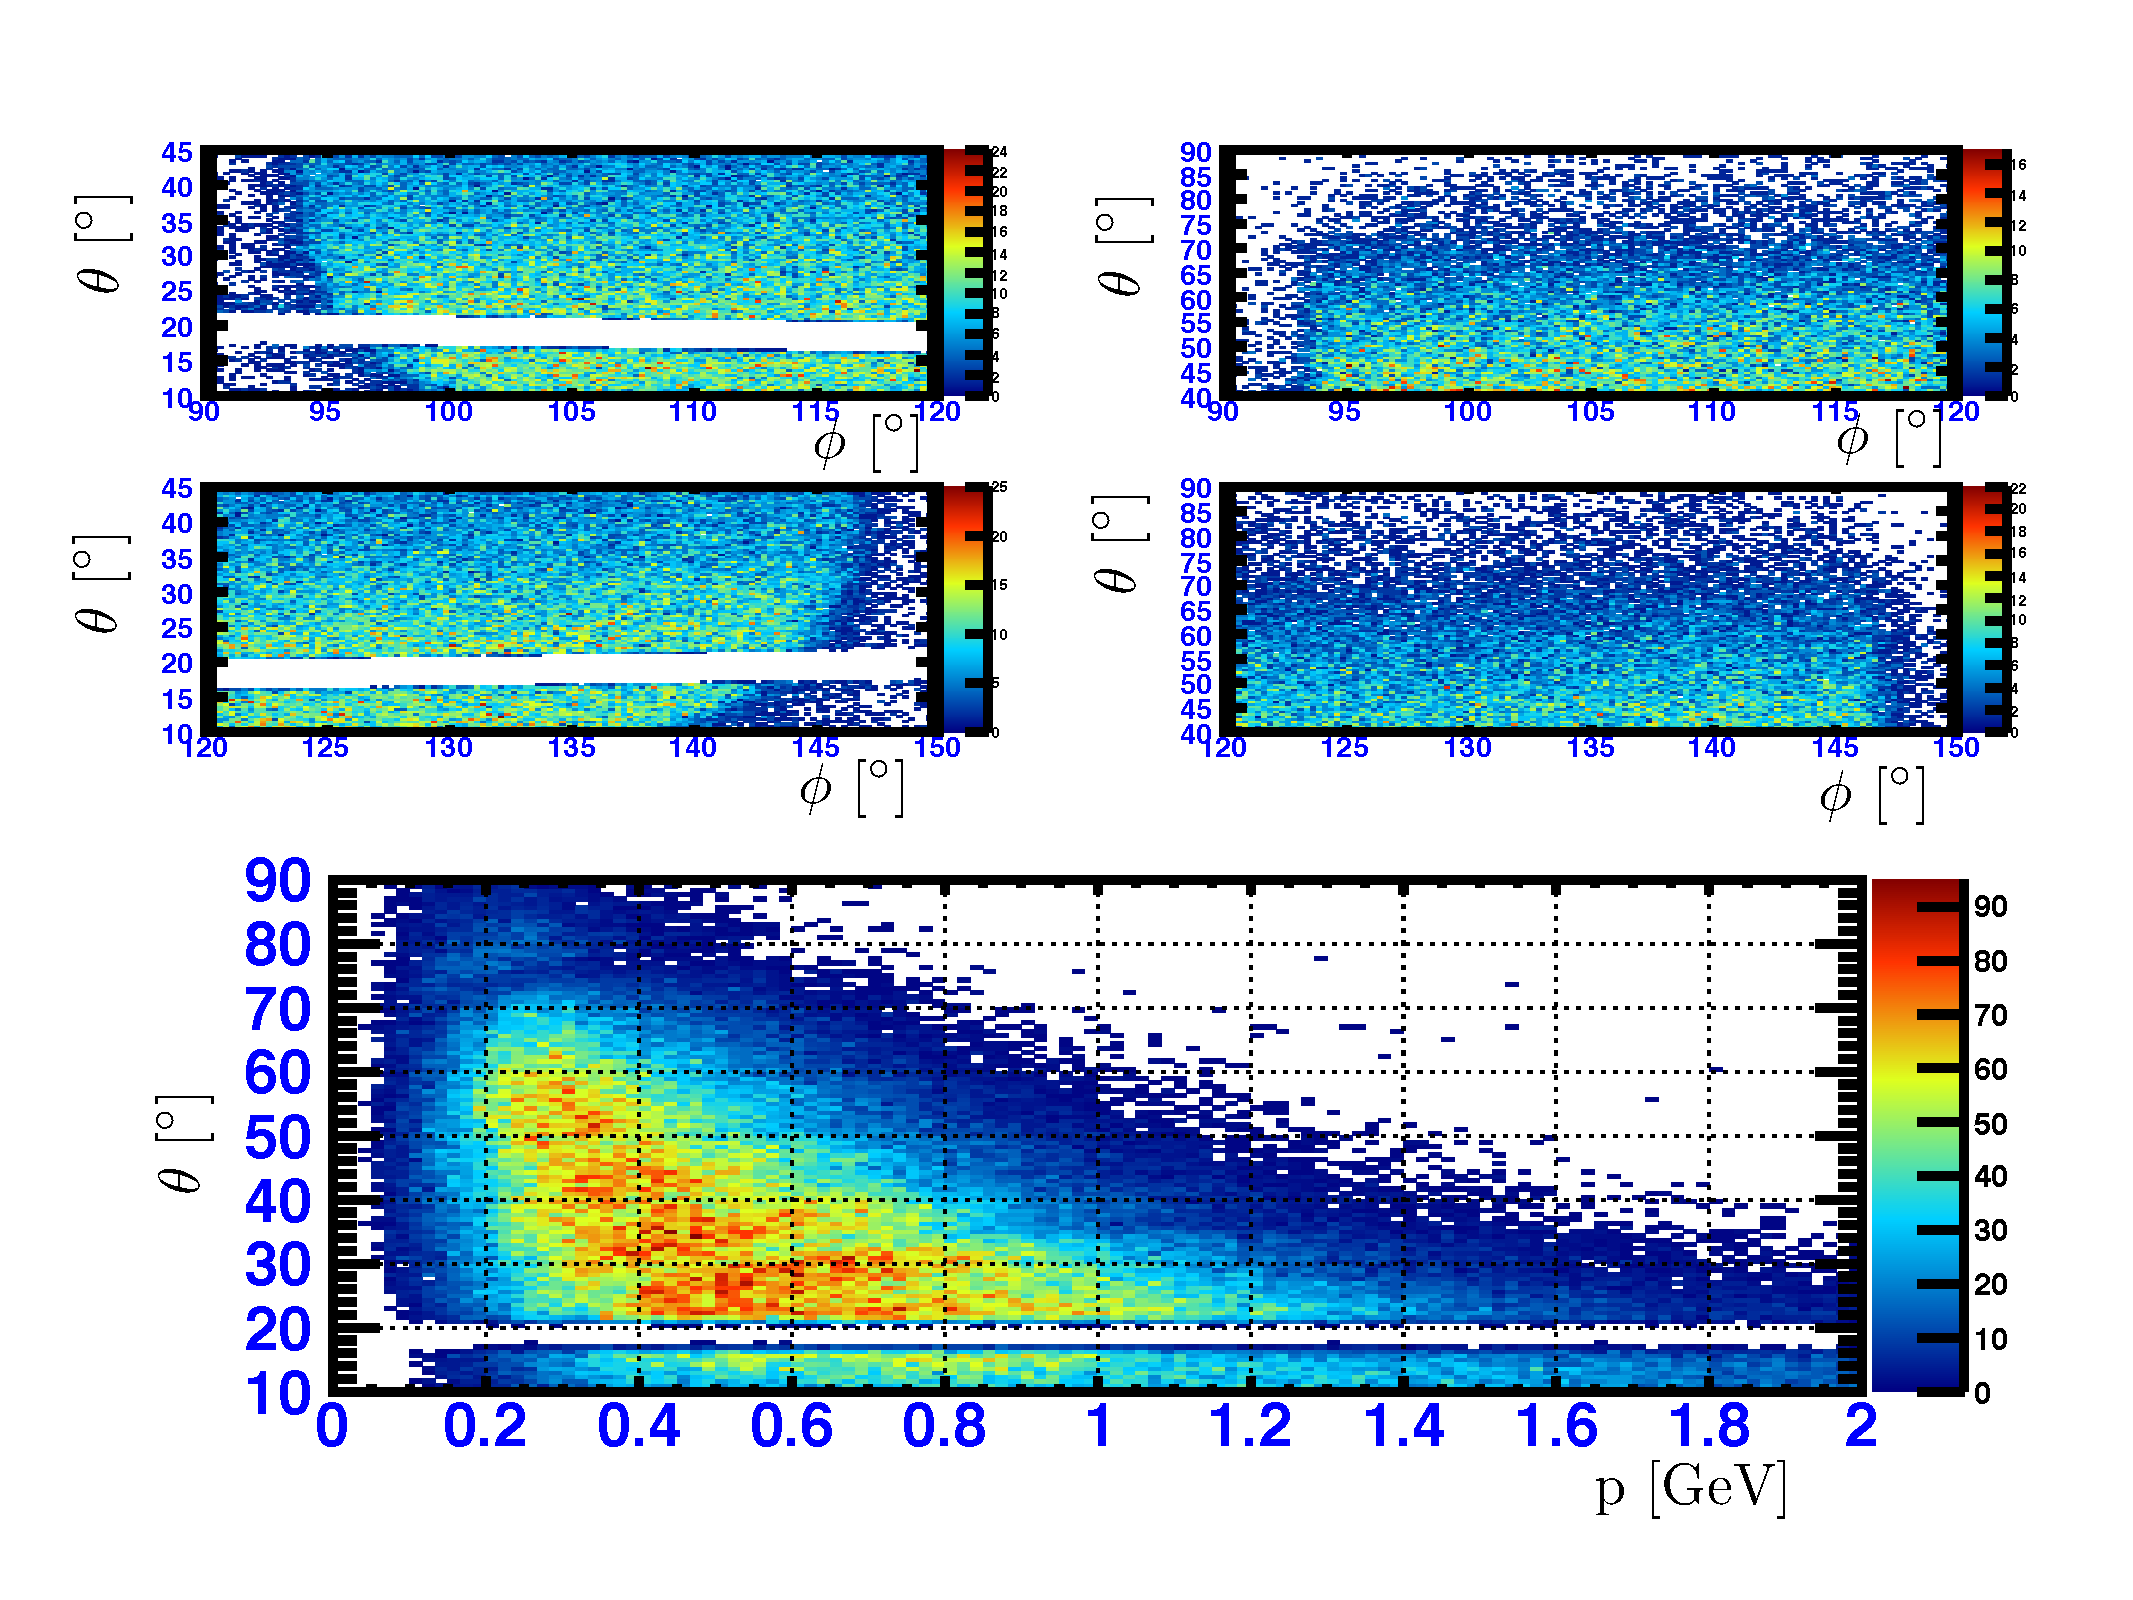
\includegraphics[width=\figwidth,height=\hfigheight]{\grpath/analysis/FIDUCIAL_CUTS/TOF/KNOCK_OUT/pip_sec3_Knockout.pdf}
\caption[Inefficiency cut for $\pi^{+} \ $ and proton data]{\label{fig:pos:tofcut_on}Inefficiency cut for $\pi^{+} \ $ and proton data. Notation same as in Fig.~\ref{fig:pos:tofcut_off}.}
\end{center}\end{figure}

\FloatBarrier
\subsection{\abbr{EC} Fiducial Cuts}\label{sec:analysis.eccc_fid}

The efficiency for the \abbr{EC} subsystem, described in Sec.~\ref{sec:clas.ec}, is different for each strip in the $u$, $v$, $w$ arrangement. As a result, there are regions of detection which are inefficient. An extreme example of this is illustrated in Fig.~\ref{fig:neg:ec.sec5}, where the \abbr{EC} \emph{inner} (top row) and \emph{outer} (bottom row) strips are plotted as a function of the azimuthal angle~($\phi$) for sector 5. A dead or inefficient strip is seen as a horizontal band in Fig.~\ref{fig:neg:ec.sec5}.  The curvature of inefficient strips seen are reflections of inefficieny in an another orientation. For example, the curves seen in the top left plot, $u$ orientation, of Fig.~\ref{fig:neg:ec.sec5} is a reflection of dead or inefficient strips from $v$ and $w$ orientations respectively.
%
\begin{figure}[h!]\begin{center}
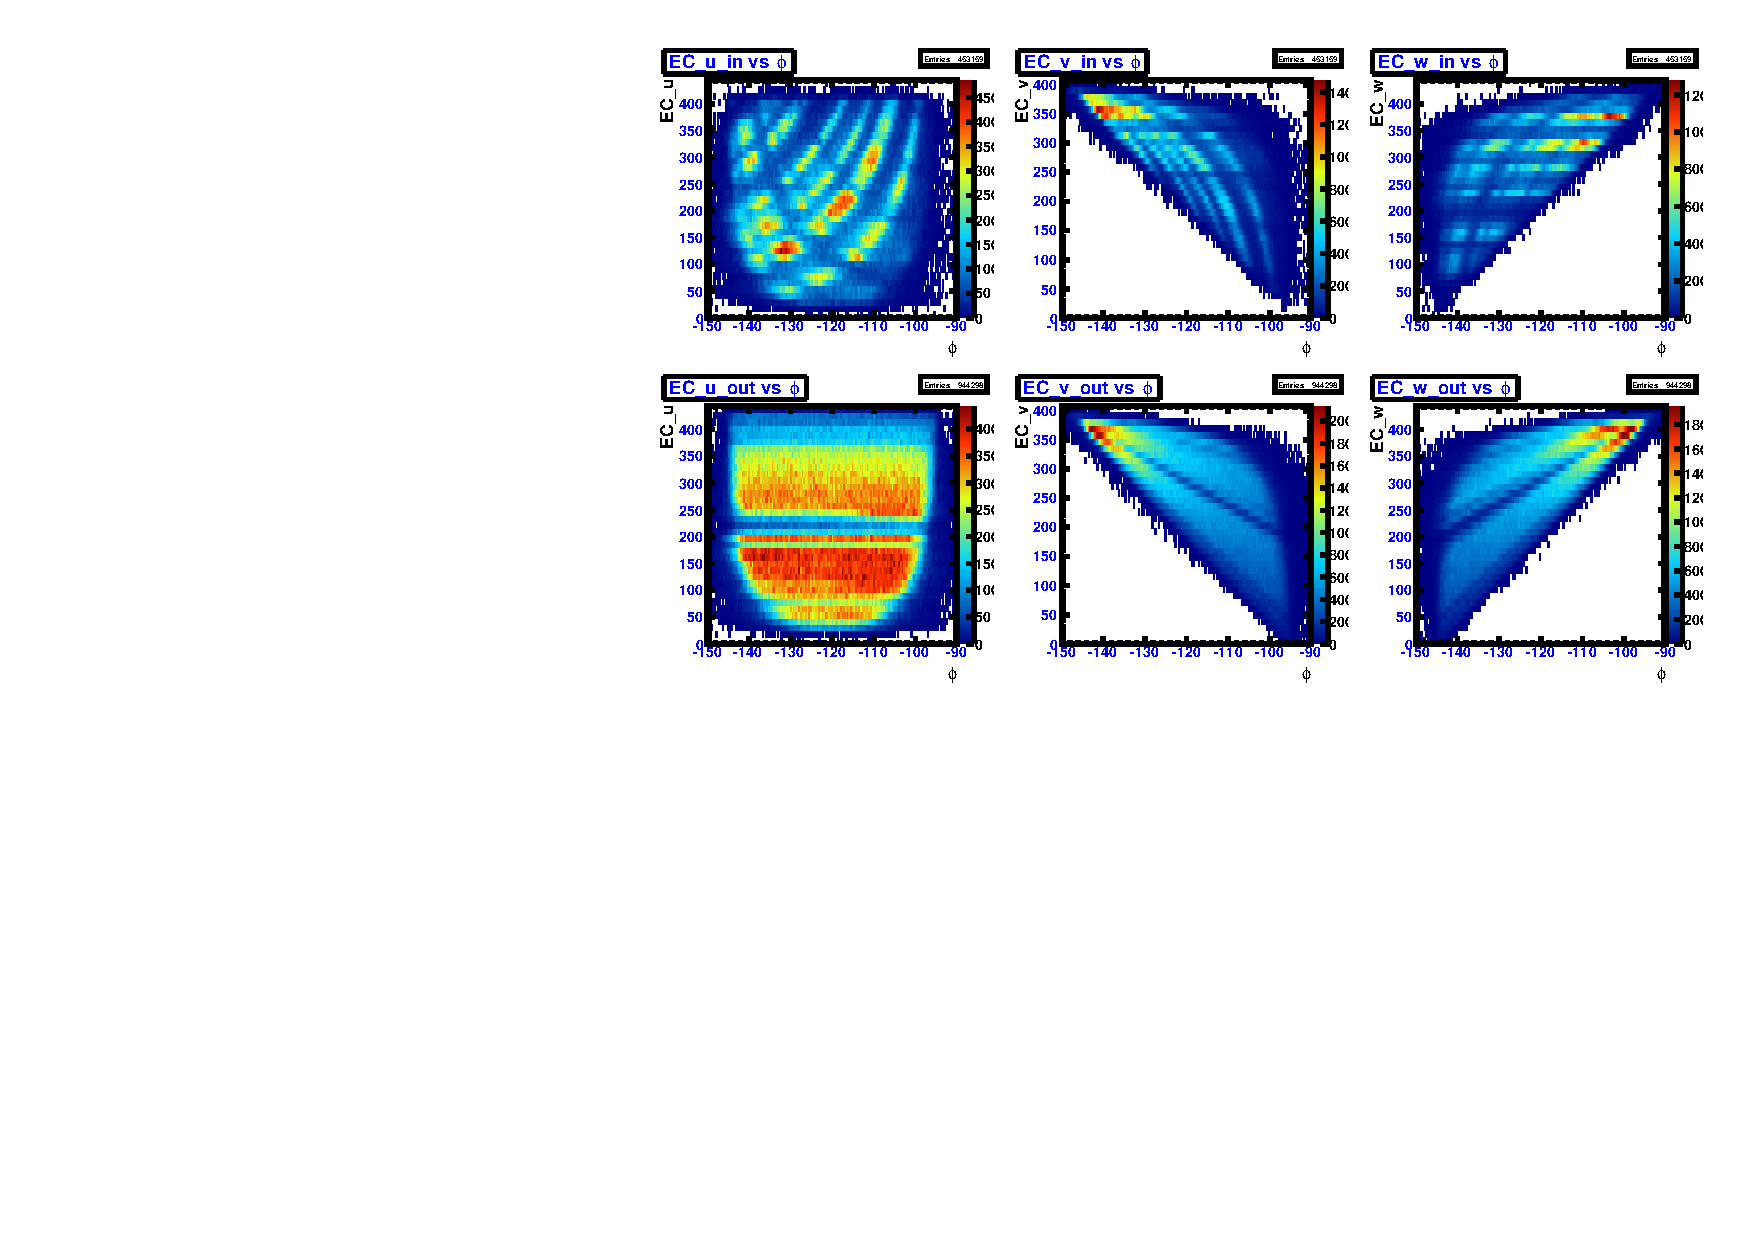
\includegraphics[width=\figwidth,height=\hfigheight]{\grpath/analysis/FIDUCIAL_CUTS/EC/pim_ecuvw_phi_NOKnockout_sec5.pdf}
\caption[Inefficient \abbr{EC} $u$, $v$, $w$ strips vs. $\phi$ for sector 5 in \abbr{CLAS} $e^{-} \ $ data]{\label{fig:neg:ec.sec5}Inefficient \abbr{EC} $u$, $v$, $w$ strips vs. $\phi$ for sector 5 in \abbr{CLAS} $e^{-} \ $ data. Top row depicts the $u$, $v$, $w$ strips for the \emph{inner} \abbr{EC}, while the bottom row depicts the $u$, $v$, $w$ strips for the \emph{outer} \abbr{EC}. The z-axis illustrates the number of hits in the plot.}
\end{center}\end{figure}
%
The projection of Fig.~\ref{fig:neg:ec.sec5} onto the y-axis can be seen in Fig.~\ref{fig:neg.ecstrip.sec5}. This view depicts the actual paddles that are dead or inefficient. It can be seen in either Figs.~\ref{fig:neg:ec.sec5} and~\ref{fig:neg.ecstrip.sec5} that there exists inefficient \abbr{EC} strips for sector 5. 
\begin{figure}[h!]\begin{center}
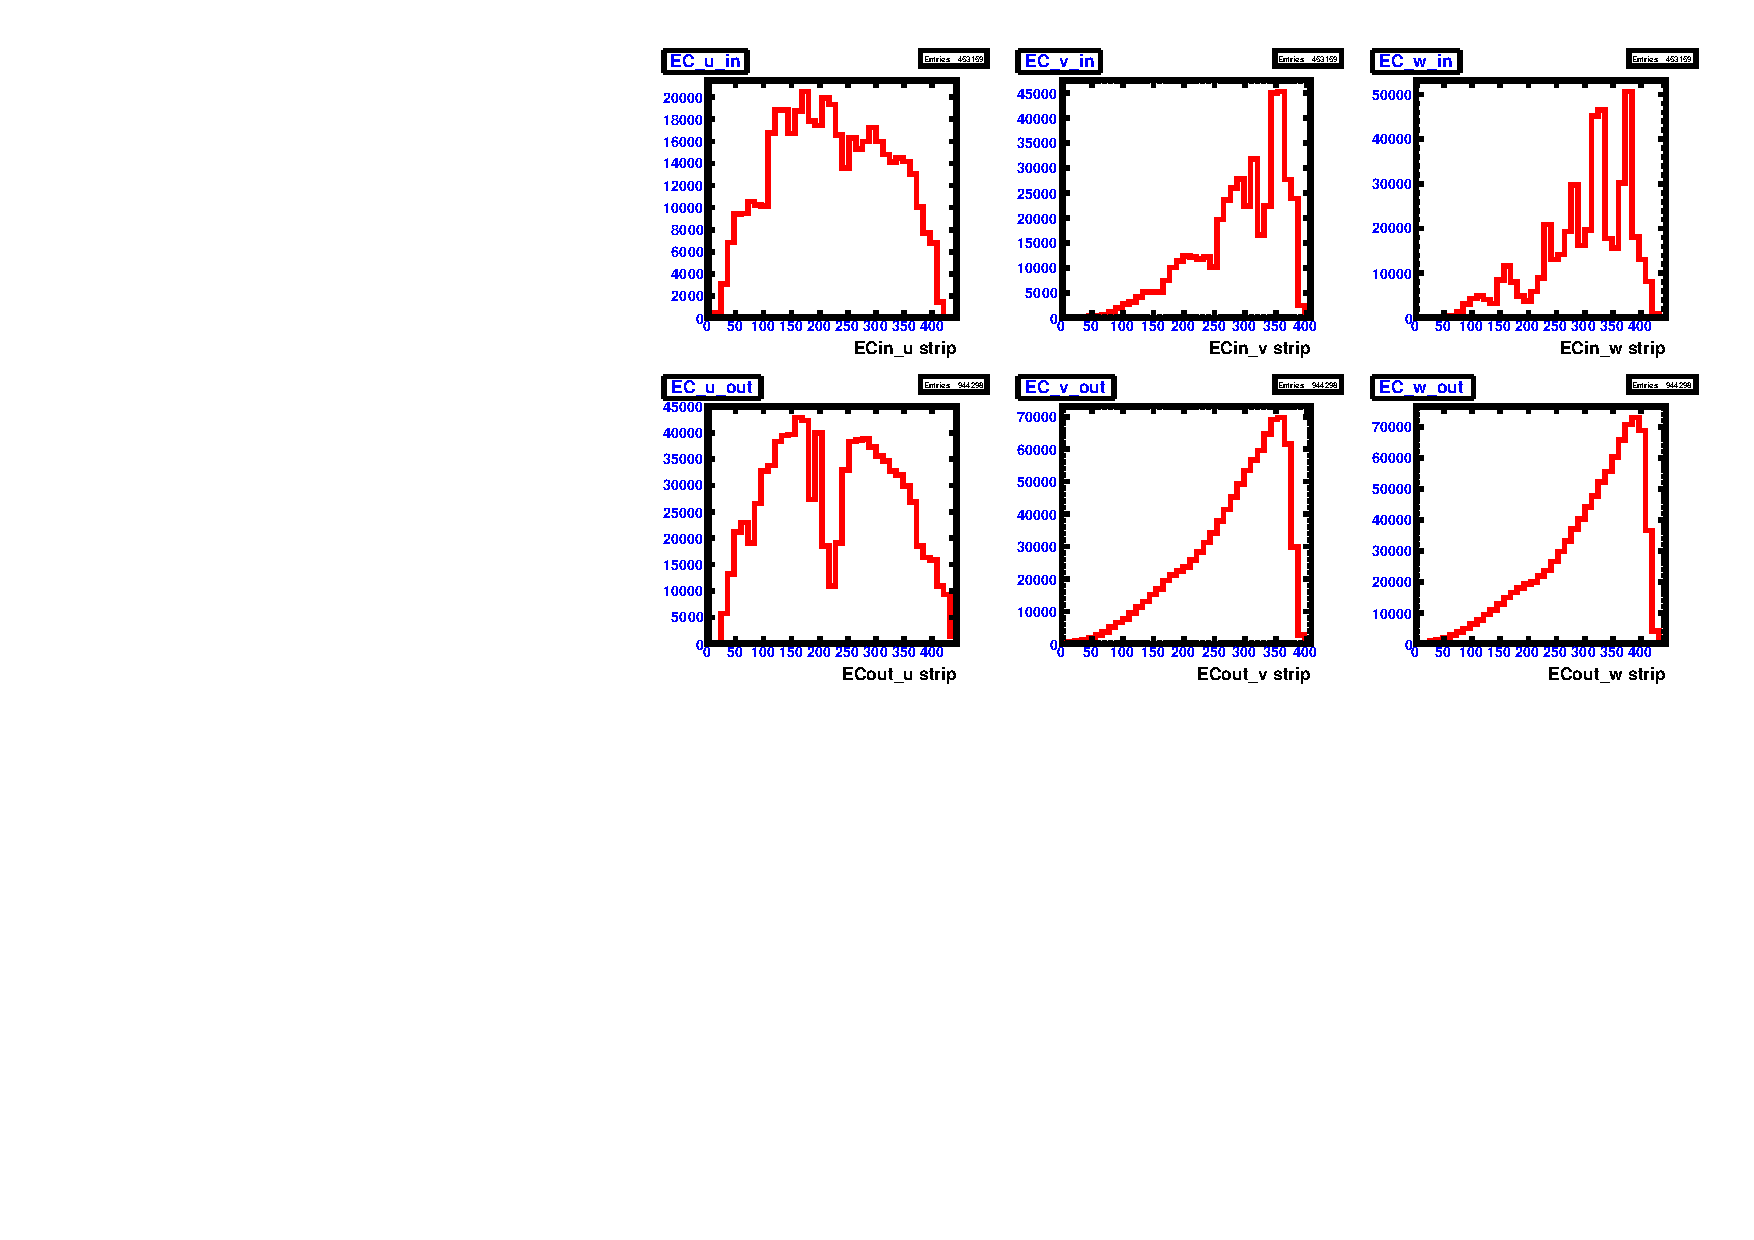
\includegraphics[width=\figwidth,height=\hfigheight]{\grpath/analysis/FIDUCIAL_CUTS/EC/pim_ecuvw_NOKnockout_sec5.pdf}
\caption[Number of hit vs. inefficient \abbr{EC} $u$, $v$, $w$ strips for sector 5 for $e^-$ data]{\label{fig:neg.ecstrip.sec5} Number of hit vs. inefficient \abbr{EC} $u$, $v$, $w$ strips for sector 5 for $e^-$ data. Top row depicts the $u$, $v$, $w$  strips for the \emph{inner} \abbr{EC}, while the bottom row depicts the $u$, $v$, $w$  strips for the \emph{outer} \abbr{EC}}
\end{center}\end{figure}
The inefficient strips were removed in data and \abbr{MC}. The effect of the inefficient strip cut, along with the standard \abbr{CLAS} \abbr{EC} geometric fiducial cuts can be seen in Fig.~\ref{fig:neg:ec.sec5_cut} and Fig.~\ref{fig:neg.ecstrip.sec5_cut}.
%
There also existed an inefficiency in other sectors. The plots to show the total inefficiency of the \abbr{EC} can be found in App.~\ref{sec:app.tof_plots}. The parameters for the \abbr{EC} strip cuts are listed in Tab.~\ref{tab:ec.eq} and the parameters for the good \abbr{EC} fiducial range can be found in Tab.~\ref{tab:ecfid.eq}.
\begin{table}[h!]
\begin{minipage}{\textwidth}
\begin{center}
\begin{singlespacing}

\caption[\abbr{EC} UVW Cut Parameters]{\label{tab:ec.eq} \abbr{EC} UVW cut parameters.}
\begin{tabular}{c|c|c}
\hline												
Sector & \abbr{EC}$_{\mathrm{\emph{inner/outer}}}$	& U  \\ \hline 	
2 & \abbr{EC}$_{\mathrm{\emph{inner}}}$ & $96\le U\le 108  \ || \  324\le U\le 336 $   \\
3 & \abbr{EC}$_{\mathrm{\emph{inner}}}$ & $324\le U\le 336  \ || \  180\le U\le 216  \ || \  324\le U\le 337 $  \\
%
2 & \abbr{EC}$_{\mathrm{\emph{outer}}}$ & $324\le U\le 336.$ \\
3 & \abbr{EC}$_{\mathrm{\emph{outer}}}$ & $131\le U\le 142  \ || \  204\le U\le 216  \ || \  324\le U\le 336 $ \\
5 & \abbr{EC}$_{\mathrm{\emph{outer}}}$ & $180\le U\le 192  \ || \  204\le U\le 240 $  \\
%
\hline
 & 	& V \\
\hline
5 & \abbr{EC}$_{\mathrm{\emph{inner}}}$  & $ 320\le V\le 342  \ || \  254\le V\le 242 $   \\
%
%
\hline
 & 	& W \\
\hline 
1 & \abbr{EC}$_{\mathrm{\emph{inner}}}$ & $312\le W\le 324$  \\
2 & \abbr{EC}$_{\mathrm{\emph{inner}}}$ & $396\le W\le 408$  \\
3 & \abbr{EC}$_{\mathrm{\emph{inner}}}$ & $ 396\le W\le 408$  \\
5 & \abbr{EC}$_{\mathrm{\emph{inner}}}$ & $ 336\le W\le 372  \ || \  288\le W\le 312  \ || \  240\le W\le 276$ \\ 
& & $  \ || \  168\le W\le 228  \ || \  132\le W\le 144$  \\
6 & \abbr{EC}$_{\mathrm{\emph{inner}}}$ & $ W\ge 396$  \\

\hline \hline%inserts single line
\end{tabular}

\end{singlespacing}
\end{center}
\end{minipage}
\end{table}
\vspace{20pt}  
\begin{table}[h!]
\begin{minipage}{\textwidth}
\begin{center}
\begin{singlespacing}

\caption[\abbr{EC} UVW Good Fiducial Parameters]{\label{tab:ecfid.eq} \abbr{EC} UVW good fiducial parameters.}
\begin{tabular}{c|c|c|c}
\hline												
\abbr{EC} Good Fiducial Range & U & V & W  \\ \hline 
& $20\le U\le 400 $  & $V\le 375.0$ & $W\le 405.0$ \\
\hline \hline%inserts single line
\end{tabular}
\end{singlespacing}
\end{center}
\end{minipage}
\end{table}
\vspace{20pt}  

\begin{figure}[h!]\begin{center}
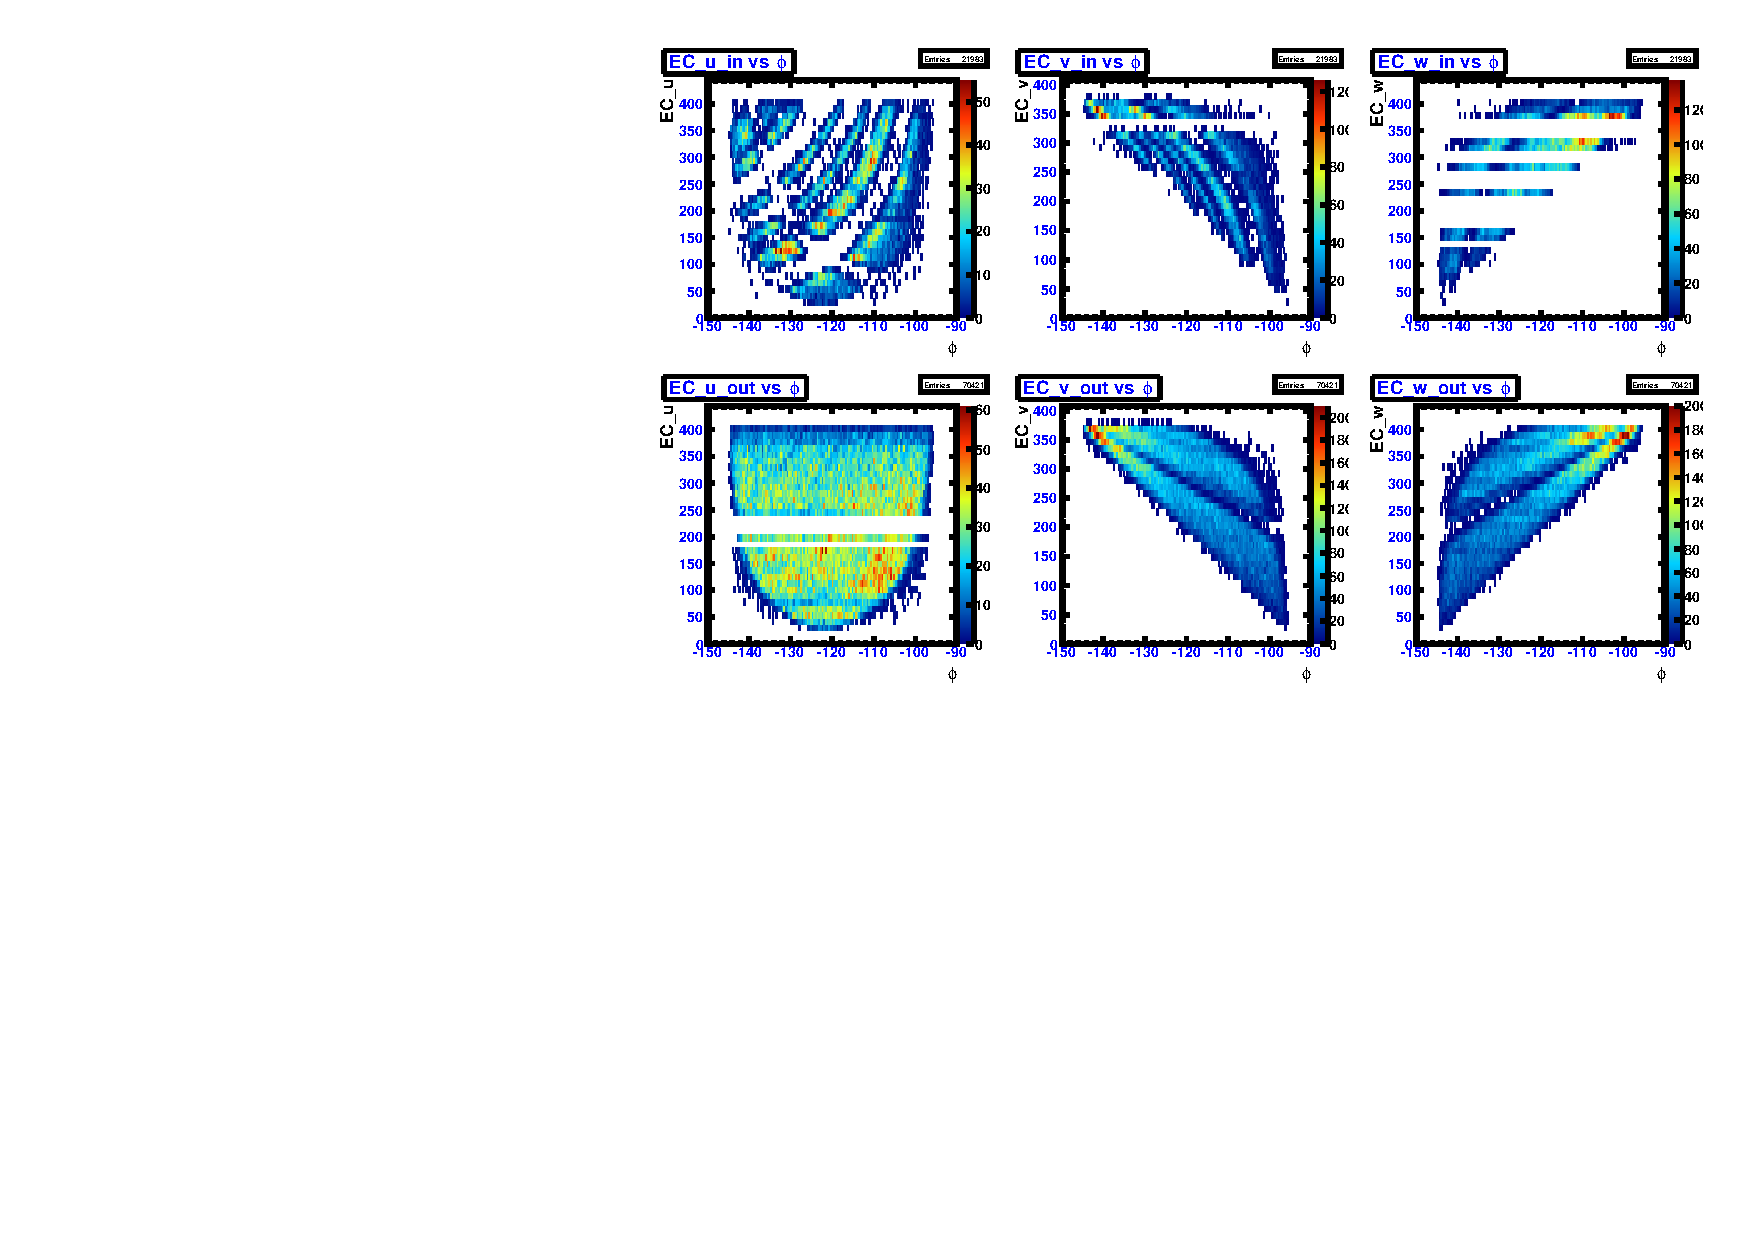
\includegraphics[width=\figwidth,height=\hfigheight]{\grpath/analysis/FIDUCIAL_CUTS/EC/pim_ecuvw_phi_afterGeoFid_sec5.pdf}
\caption[\abbr{EC} $u$, $v$, $w$ strips vs. $\phi$ for sector 5 with fiducial cuts and inefficient paddle knockouts applied to $e^-$ data]{\label{fig:neg:ec.sec5_cut} \abbr{EC} $u$, $v$, $w$ strips vs. $\phi$ for sector 5 with fiducial cuts and inefficient paddle knockouts applied to $e^-$ data. Top row depicts the $u$, $v$, $w$ strips for the \emph{inner} \abbr{EC}, while the bottom row depicts the $u$, $v$, $w$ strips for the \emph{outer} \abbr{EC}. The z-axis illustrates the number of hits in the plot.}
\end{center}\end{figure}
%
\begin{figure}[h!]\begin{center}
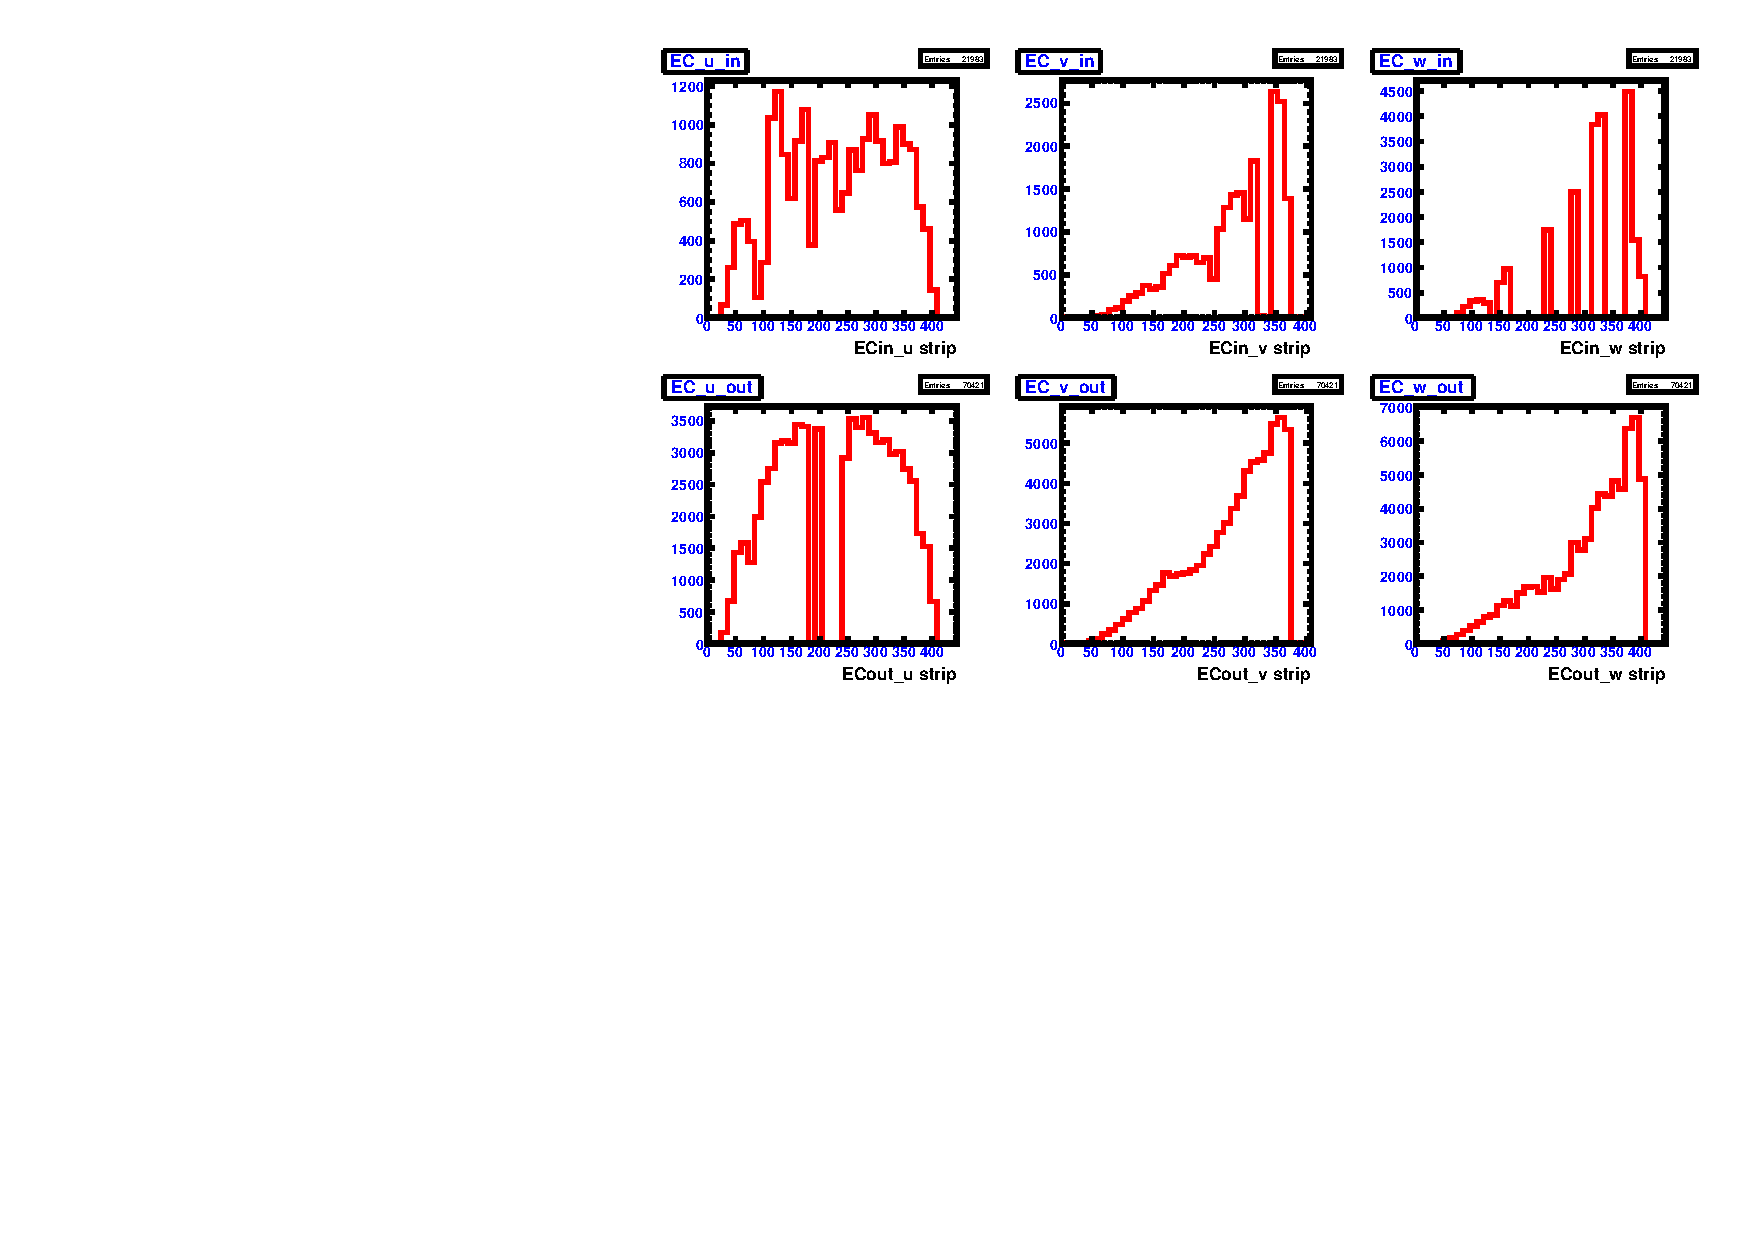
\includegraphics[width=\figwidth,height=\hfigheight]{\grpath/analysis/FIDUCIAL_CUTS/EC/pim_ecuvw_afterGeoFid_sec5.pdf}
\caption[Number of hits vs. \abbr{EC} $u$, $v$, $w$ strips for sector 5 with fiducial cuts and inefficient paddle knockouts applied to $e^-$ data]{\label{fig:neg.ecstrip.sec5_cut}Number of hits vs. \abbr{EC} $u$, $v$, $w$ strips for sector 5 with fiducial cuts and inefficient paddle knockouts applied to $e^-$ data. Top row depicts the $u$, $v$, $w$ strips for the \emph{inner} \abbr{EC}, while the bottom row depicts the $u$, $v$, $w$ strips for the \emph{outer} \abbr{EC}}
\end{center}\end{figure}

\FloatBarrier


\section{Simulation}\label{sec:analysis.simulation}
There are certain kinematic regions of \abbr{CLAS} in which physics events are not being recorded properly i.e.~the area dividing each sector in \abbr{CLAS}. Furthermore each sector in \abbr{CLAS} is asymmetric in the acceptance of events due to subsystem inefficiencies such as inoperable \abbr{DC} wires, \abbr{PMT} inefficiencies, dead scintillator strips the the \abbr{TOF} and \abbr{ST} subsystems. When a triggered event is recorded and reconstructed these asymmetric inefficiencies factors are reflected and must be carefully understood because these factors are properties of the \abbr{CLAS} detector and independent of any physics that occurred. To properly understand the detector effects on the data, \abbr{CLAS} utilizes a \abbr{GEANT} simulation package know as \abbr{GSIM}. To prepare an event for \abbr{GSIM} the program \abbr{GAMP2PART} converts a text file, containing the 4-momentum of the generated event, into a suitable file format for \abbr{GSIM}. \abbr{GSIM} then simulates the passage of these particles through the \abbr{CLAS} detector and generates the associated \abbr{ADC} and \abbr{TDC} information from detector hits. \abbr{GSIM} takes into account detector inefficiencies described in the \abbr{\texttt{CLAS\_CALDB\_RUNINDEX}}. The \abbr{CLAS\_CALDB\_RUNINDEX} is an array of information about each subsystem's inefficiency that was derived during the \g12 calibration process. The \abbr{GSIM} simulated hits are then ``post-processed'' by smearing the \abbr{TDC} and \abbr{ADC} hits to imitate the observed resolution of the detector subsystems using the program \abbr{GPP} (\abbr{GSIM} post-processor). \abbr{GPP} also removes detector hits due to inefficient \abbr{DC} wires. The simulation output processed with \abbr{GPP} is then reconstructed with \texttt{a1c}, the same program used to reconstruct data events. The reconstructed simulation is subject to the same scrutiny as real data events, undergoing all the cuts (Sec.~\ref{sec:analysis.data.reduction}), corrections (Sec.~\ref{sec:analysis.corrections}), and kinematic fitting (Sec.~\ref{sec:analysis.fitting}), as the real data except for beam corrections (Sec.~\ref{sec:analysis.corrections.beam}).

\subsection{Simulation Verification}\label{sec:analysis.accept.verify}
Part of understanding the simulation output is understanding how well the simulation mimics the real data. To investigate this, 26000 real \epem events were treated as generated events and inputted into the \abbr{GAM2PART}$\to$\abbr{GSIM}$\to$\abbr{GPP}$\to$\texttt{a1c} chain. Of the 26000 inputted, only 100 were successfully reconstructed through the simulation chain. The source of this low efficiency was due to the calibrations entries for the \abbr{CC} and \abbr{EC} in the \abbr{CLAS\_CALDB\_RUNINDEX} not having values in which would set the ``PEDESTAL'' values appropriately for simulation. The calibrations constants in the \abbr{CLAS\_CALDB\_RUNINDEX} were correct for data reconstruction, but not for simulation reconstruction of \epem in the \abbr{CC} and \abbr{EC} subsystems. It was also discovered that the \abbr{CC} and \abbr{EC} subsystems should be simulated with ``RUN 10'' constants instead of the normal ``RUN 56855'' used by the \g12 group. ``RUN 56855'' is a special run benchmarked to have the best calibrations and required to properly simulate the \abbr{ST}, \abbr{DC}, and \abbr{TOF} subsystems. To rectify this, a special \abbr{CLAS\_CALDB\_RUNINDEX} was created, changing ``RUN 10'' for to have ``RUN 56855'' constants for all subsystems except the \abbr{CC} and \abbr{EC} subsystems which were kept at ``RUN 10'' constants. Inputting the 26000 real \epem events into the simulation chain using the \abbr{CLAS\_CALDB\_RUNINDEX} \emph{RunIndexg12\_leptons\_and\_photons} outputted $\approx$~24700 \epem reconstructed events, a $\approx$~95~\% efficiency.

The missing 5~\% was a result of ``time-based'' and ``hit-based'' tracking failures as briefly mentioned in Sec.~\ref{sec:data.cook}. The events that failed ``hit-based'' tracking contributes a 3.75~\% overall event inefficiency. The cause of the ``hit-based'' failure was never determined, but it was thought to have also occur in the cooking of the data. Therefore since it did occur in the data reconstruction this was considered to cancel the inefficiency of the simulation.

The ``time-based'' failure was due to a random bug in the processing of the \abbr{TDC} element information of \abbr{ST} (\abbr{STN0}) and the \abbr{ADC} element information of \abbr{ST} (\abbr{STN1}) raw data banks. The bug miscalculated the tracks sector exiting the \abbr{ST} even as the hit element of the \abbr{ST} matched that to the track in the \abbr{DC}. If the track failed due to this error, it usually passed ``time-based'' on the second or third pass of the ``time-based'' tracking if another particle passed ``time-based'' during the initial pass. The probability that a track failed initial ``time-based" tracking was $\approx$~.23\%. The probability that this failed event would pass ``time-based" tracking after another pass was $\approx99.78\%$. The average inefficiency for three charged track events for data was 0.0125\%

%This inefficiency depends on the distance the track is from the z-vertex position and can be seen in Fig.~\ref{fig:classt.ineffII}.
%\begin{figure}[h!]\begin{center}
%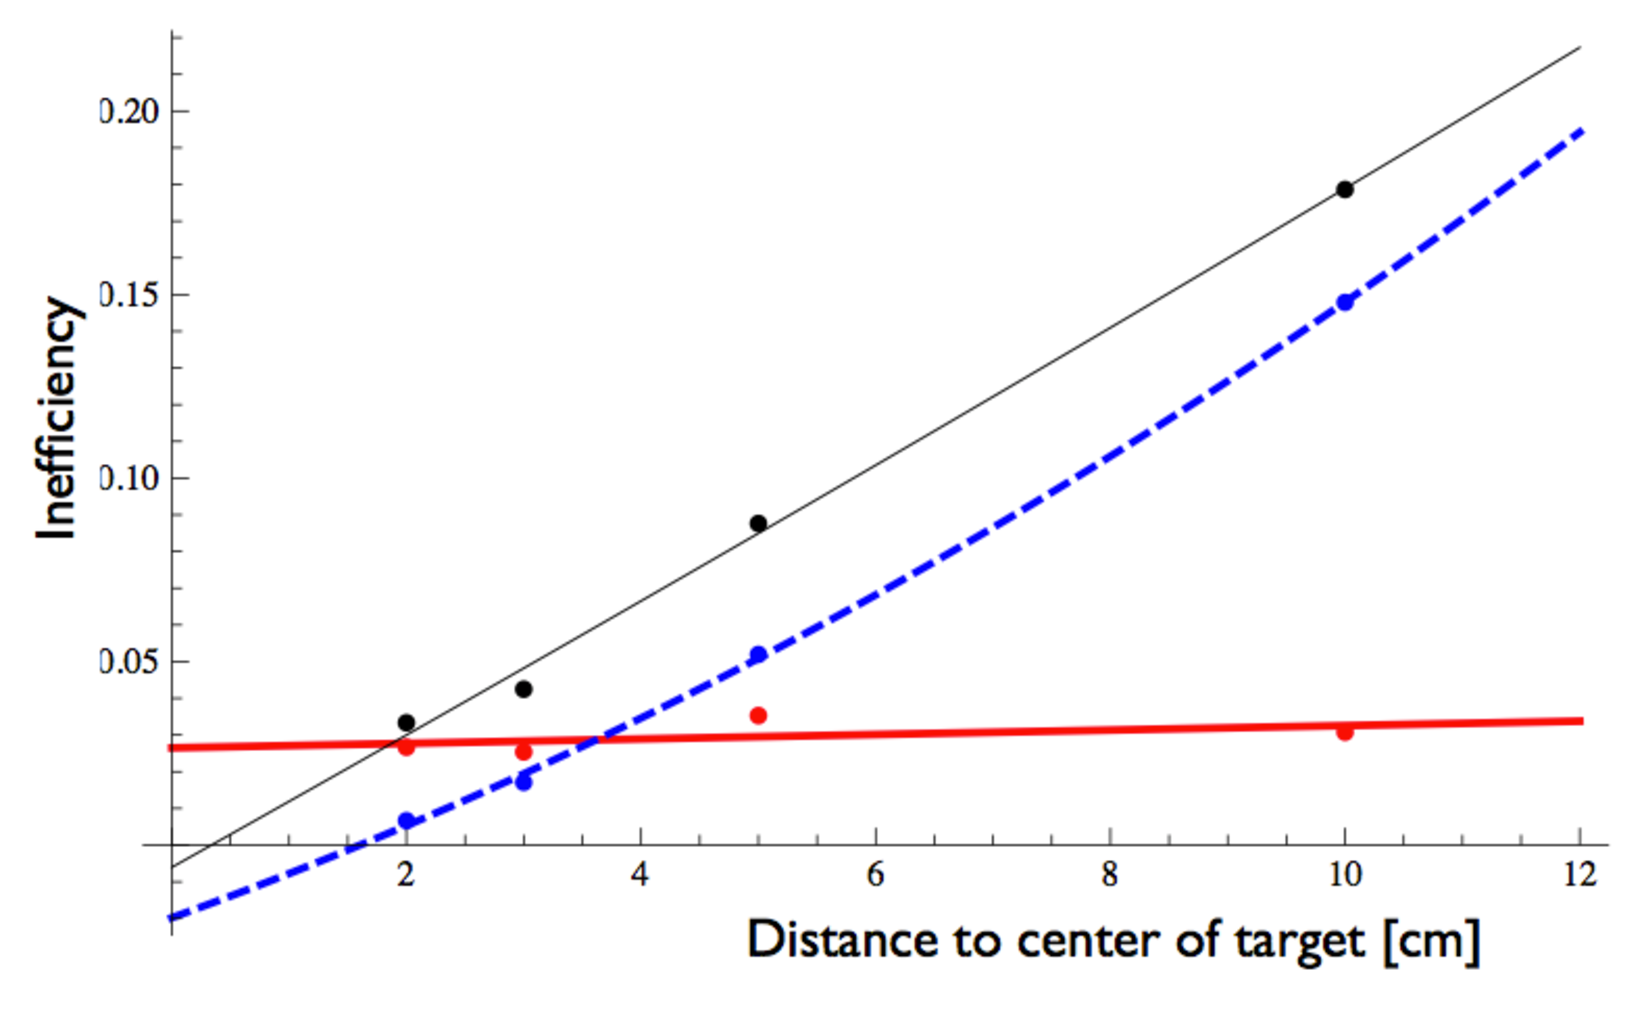
\includegraphics[width=0.8\figwidth,height=0.7\qfigheight]{\grpath/hall-b/st_issue_4_thesis.pdf}
%\caption[Start Counter Inefficiency]{\label{fig:classt.ineffII}{\coloronline}Plot showing the inefficiency of the start counter from data events, red-solid line is the inefficiency of reconstruction based solely on hit-based tracking, blue-dashed line is inefficiency of start counter, black-solid is combined. }
%\end{center}\end{figure}

\FloatBarrier
\subsection{Simulating the Lepton Trigger}\label{sec:analysis.accept.trigger}
During the collection process, for an event to be written by the \abbr{DAQ} it must have passed at least one of the trigger ``bits" defined in Sec.~\ref{sec:clas.g12.conditions.data}. As discussed in Sec.~\ref{sec.data.trig.lepton}, the process of lepton triggering required a coincidence between the \abbr{EC} and the \abbr{CC} subsystems. This coincidence was established by using the voltage sum of the \abbr{CC} for a sector and the voltage sum of the \abbr{EC} for the same sector and comparing each sum to a preset threshold described in Table~\ref{tab:data.ecccthresh}. However when \abbr{GSIM} simulates tracks through the \abbr{CC} and \abbr{EC}, it does not account for the minimum voltage threshold that was required for data collection, moreover the simulation of the trigger must match the trigger efficiency discussed in Sec.~\ref{sec:analysis.trigger.verify}.

Simulation of the \abbr{CC} and \abbr{EC} trigger ``bit 6'', Sec.~\ref{sec.data.trig.lepton}, was performed by writing an algorithm that attempted to mimic the method in which triggered data was recorded. To accomplish this a modified function, written by Simeon McAleer from FSU, was written into the simulation reconstruction algorithm. The routine returned the sector and a boolean of 0 or 1 (pass or fail), that simulated the trigger based on the following criteria;
\begin{enumerate}\label{trig:sim.all}
\item The sector with the highest EC summed energy over threshold. \label{trig:sim.ECtot} 
\item The sector with the highest EC Inner Layer summed energy over threshold. \label{trig:sim.ECinner} 
\item The sector with the highest CC summed energy over threshold. \label{trig:sim.CCtot} 
\item All three above conditions must be in same sector.
\end{enumerate}
Thresholds as described in Table~\ref{tab:data.ecccthresh} are 80~mV, 60~mV and 20~mV for \abbr{EC} \emph{inner}, \abbr{EC}\emph{total} and CC respectively. The \abbr{CC} trigger threshold was applied to groups of eight \abbr{CC} \abbr{PMT}s, called ``sim bits''. The ``sim bits'' were staggered by four \abbr{PMT}s so that each \abbr{PMT} goes into two ``sim bits'', after which all ``sim bits'' were ``\emph{OR}'''d together. If any ``sim bit'' calculated as above threshold, that specific sector was then compared to the remaining sectors to establish the condition listed in~\ref{trig:sim.CCtot}.

The \abbr{EC} \emph{inner} and \abbr{EC} \emph{total} trigger thresholds were applied to all \abbr{EC} strips in a sector. This was done by summing over the energy for every strip in every orientation of the \abbr{EC} per sector. If the energy summation for the \abbr{EC} \emph{inner} was above threshold,   that specific sector was then compared to the remaining sectors to establish the condition listed in~\ref{trig:sim.ECinner}. If the energy summation for the \abbr{EC} \emph{total} was above threshold, that specific sector was then compared to the remaining sectors to establish the condition of the sector with the highest EC summed energy over threshold.

\subsubsection{Validity of Trigger Simulation}
The actual triggered data could have been triggered by the following sceneries;
\begin{enumerate}\label{trig:get.all}
\item $e^-$ \abbr{CC} and \abbr{EC} hit above preset thresholds,
\item $e^+$ \abbr{CC} and \abbr{EC} hit above preset thresholds,
\item $e^-$ \abbr{CC} hit above preset thresholds and $e^+$ \abbr{EC} hit above preset thresholds in the same sector, 
\item $e^-$ \abbr{EC} hit above preset thresholds and $e^+$ \abbr{CC} hit above preset thresholds in the same sector. 
\end{enumerate}
The lepton trigger ``bit 6" was 100\% efficient (see Sec.~\ref{sec:analysis.trigger.verify}) when the data was cut using all the conditions listed above (1, 2, 3, 4) using an ``OR" flag. This means that a $\gamma p \to p e^+ e^-$ event must satisfy at least one of the listed conditions. The reduction in events when at least one of the conditions was satisfied was 69.91\%. Prior to simulating the trigger, cutting the \abbr{MC} with the listed conditions reduced the event yield by 81.91\%. Simulating the trigger and cutting on the \abbr{MC} events with the listed conditions reduced that event yield to 69.48\%. This indicates that the trigger simulation is properly mimicking the trigger configuration used when data is collected. 

%actual physics events recorded by \abbr{CLAS}.
%
%
%When all the conditions listed above are compared together using an ``\emph{OR}'' flag, on \piz data, 69.91\% of events remain. To check the validity of the trigger simulation, events from the \piz reconstructed simulation were placed under the conditions as the actual data. Without placing the boolean of 1 on the simulation, 81.91\% of events remain. Placing the boolean of 1 on the simulation, 69.48\% of events remain, indicating the trigger simulation is mimicking the actual physics events recorded by \abbr{CLAS}. 





\section{PLUTO++ Event Generator}\label{sec:pluto}

Pluto~\cite{PLUTO} is a Monte-Carlo event generator designed for the study of hadronic interactions and heavy ion reactions in \abbr{HADES}, \abbr{FAIR} and upcoming \abbr{PANDA} collaborations. The versatility of Pluto enables its use as an event generator for photoproduction in \abbr{CLAS}. For hadronic interactions, Pluto can generate interactions from pion production threshold to intermediate energies of a few~GeV per nucleon. The entire software package is based on ROOT and uses ROOT's embedded C++ interpreter to control the generation of events. Programming event reaction can be set up with a few lines of ROOT macro code without detailed knowledge of programming. Some features in Pluto are, but not limited to;
\begin{itemize}
\item Ability to generate events in phase space.
\item Ability to generate events with a continuous bremsstrahlung photon beam.
\item Ability to generate events weighted by a user defined $t$-slope.
\item Ability to generate events weighted by a user defined cross-section.
\begin{itemize}
\item Total cross section can be inputted via functional form or histogram.
\item Differential cross sections can be inputted via functional forms or histograms for specific beam energies up to 110 histograms relating to intervals of beam energy.
\end{itemize}
\item Ability to generate events that decay via already established physics parameters, i.e.~transition form factors.
\item Ability to generate events that decay via modified established physics parameters.
\item Ability to generate events with multiple production channels, weighted by user inputted cross-section probability.
\item Ability to generate events with multiple decay channels, weighted by user inputted branching ratio.
\item Ability to perform vertex smearing.
\item Ability to create virtual detectors.
\end{itemize}

For the analysis presented in this work, Pluto was used in conjunction with known differential cross sections to verify simulation momentum smearing and tagger resolution, Sec.~\ref{sec:analysis.simsmear.verify}. Pluto was also utilized as a phase space generator in this analysis, to perform a ``tune'' on the kinematic fitter, Sec.~\ref{sec:analysis.fitting}, to calculate the acceptance corrections Sec.~\ref{sec:results.acceptance}, and to calculate the normalization Sec.~\ref{sec:results.normalization}.
\section{Kinematic Fitting}\label{sec:analysis.fitting}
When \abbr{CLAS} records a triggered event, there is always an error associated with the measurement of the vector $\vec{\eta}$ in the form of,
\begin{align}
\vec{\eta}  = \vec{y} + \vec{\epsilon} \ ,
\end{align}
where $\vec{y}$ are the actual values that would have been measured by CLAS in the absence of measurement errors $\vec{\epsilon}$. To improve the precision of the measurement on $\vec{\eta}$, kinematic fitting is used to impose kinematic constraints by using the method of Lagrange multipliers to perform a least-squares fit of a hypothesis. The hypothesis is dictated by physics constraints, e.g. conservation of 4-momenta. Depending on the physics of interest, the kinematic fitter is able to solve for constraint fits listed in Table~\ref{tab:fitting.constraint}. In Table~\ref{tab:fitting.constraint}, the ``Topology'' column lists the physics of interest with the constraint particle in parenthesis while the ``Extra Constraint'' column lists a secondary inputted constraint used in the fitting process. 
\begin{table}[h!]
{
\centering
\begin{minipage}{\textwidth}
%\begin{center}
\begin{singlespacing}

\caption[Examples of Constraint Fits ]{\label{tab:fitting.constraint}Examples of constraint fits \vspace{0.75mm}}
%γp → K+Σ∗0 → K+Λπ0 → K+pπ−π0 with the notion that the only thing needed to kinematically fit is the p-π−

\begin{tabular}{c|c|c} \hline
%%%%%% Title row starts here
Type of Fit & Topology &Extra Constraint \\ \hline
%%%%%% Row Foo starts here
4-C & $\gamma p \rightarrow p \pi^+\pi^-$ & -  \\
1-C & $\gamma p \rightarrow p e^+e^- (\gamma)$ & - \\
2-C & $\gamma p \rightarrow p e^+e^- (\gamma)$ & $e^+e^- (\gamma) \rightarrow \pi^0$ \\
2-C & $\gamma p \rightarrow K^+\Sigma^{*0}  \rightarrow K^+\Lambda(\pi^0) \rightarrow K^+p\pi^-(\pi^0)$ & $p\pi^- \rightarrow \Lambda$   \\
\hline\hline
\end{tabular}


\end{singlespacing}
%\end{center}
\end{minipage}
}
\end{table}
\vspace{20pt}
The method of kinematic fitting is described in great detail in~\cite{dustin.kinfit}. The kinematic fitter used in \g12 analyses has been written by Dustin Keller~\cite{dustin.kinfit}.
% 
\subsubsection{Confidence Levels and Pull Distributions}
Using the kinematic fitter to select events requires the determination of a ``quality of fit'' for a given physics hypothesis. The ``quality of fit''  is the minimization quantity interpreted from the $\chi^2$ distribution of ($q$ - $d)$ degrees of freedom, where $q$ is the number of measurements and $d$ is the number of unknown parameters. The systematic measure of probability that a $\chi^2$ of the ideal theoretical distribution is greater than or equal to the $\chi^2$ value found from the fit for a full distribution of events is defined as a``confidence level'' and expressed as 
\begin{align}
P(\chi^2)=\int^{\infty}_{\chi^2}f(x,n)dx
\end{align}
where the function $f(x,n)$ is the $\chi^2$ probability density function for $n$ degrees of freedom. ``Confidence levels'' range flat and even from $0<P(\chi^2)<1$  when the fit hypothesis is satisfied, correspondingly the ``confidence level''  is small for events that are poorly described by the fit hypothesis.
The method of checking the quality of the covariance matrix and ensuring the kinematic fit is working properly was done by examining the ``pull" distributions for quantities of a ``test fit'', see Sec.~\ref{analysis.fitting.tune}. The pull distribution is defined as the difference between the measured and the final parameters obtained by the kinematic fit and normalized by the quadratic error difference~\cite{dustin.kinfit}. Defining $\vec{\eta_i}$ and $\vec{\eta_f}$ as the initial and final vector values of the measured quantities and  $\sigma_{\vec{\eta_i}}$ and $\sigma_{\vec{\eta_f}}$ as the errors of vectors $\vec{\eta_i}$ and $\vec{\eta_f}$, the pull distribution is defined as,
\begin{align}
\vec{z} = \frac{\vec{\eta_i} - \vec{\eta_f}}{\sqrt{\sigma_{\vec{\eta_i}}^2 - \sigma_{\vec{\eta_f}}^2}} \ .
\end{align}
%
If the covariance matrix errors are correctly estimated, the pulls will be normally distributed with zero mean and have a unit standard deviation.
\subsubsection{Tuning}\label{analysis.fitting.tune}
In order for the kinematic fitter to perform a $\chi^2$ minimization properly, it has to be provided with an initial covariance matrix that contains the correlations between the kinematic variables of each track as determined during the reconstruction of the track. The covariance matrix recorded by \abbr{CLAS} is inadequate to use in the kinematic fitter because the covariance matrix does not incorporate multiple scattering errors, ``energy loss'' or the error approximation is misrepresented by a systematic. To correct for this, the elements of the covariance matrix are scaled appropriately by the kinematic fitter routine by means of what is called ``tuning''. The process of ``tuning'' determines the nature of the misrepresented errors as a function of a measured variable by studying the shift from the zero mean at different ranges of dependent variables. To perform a ``tune'', a test channel must be chosen in which the event selection must be background free. The multiple scattering option used in this analysis was set to false, therefore an algorithm which attempts to incorporate multiple scattering is not utilized. Instead a directory of parameterization files are called for the scaling of individual particle covariance matrix elements, such as $p$, $\pi^+$, $\pi^-$, $e^+$ and $e^-$. This was done because the multiple scattering algorithm did not perform well for events involving electrons and positrons. 

For this analysis, the channels
\begin{align}
\gamma p \rightarrow \pi^+ \pi^- (p) \label{eq:fit.ptune}\\
\gamma p \rightarrow p \pi^- (\pi^+) \label{eq:fit.piptune}\\
\gamma p \rightarrow \pi^+ p (\pi^-) \label{eq:fit.pimtune}\\
\gamma p \rightarrow p \omega/\rho \rightarrow p e^+ e^- \label{eq:fit.leptune}
\end{align}
%
were chosen as the ``tune'' channels because these channels incorporate the physics and background of the analysis performed. The reactions ~\ref{eq:fit.ptune},~\ref{eq:fit.piptune},~\ref{eq:fit.pimtune} were ``tunes'' done individually for the proton, $\pi^+$ and $\pi^-$ respectively, while ~\ref{eq:fit.leptune} ``tuned'' the electrons and positrons together because of the limit in statistics needed to tune each lepton individually. Once the ``tuning'' for~\ref{eq:fit.ptune},~\ref{eq:fit.piptune},~\ref{eq:fit.pimtune} was complete, the ``tune'' was verified by checking the pull distributions and confidence level for the topology,
\begin{align}
\gamma p \rightarrow p \pi^+ \pi^- \label{eq:fit.ppippimtune} \ .
\end{align}
Figures~\ref{fig:kinfit.LepPullData} and~\ref{fig:kinfit.LepPullMC} illustrate the quality of the ``tuned'' covariance matrix for \g12 data and \g12 simulation of electrons and positrons from ``tune''~\ref{eq:fit.leptune} and Fig.~\ref{fig:kinfit.LepPullProb} illustrates the ``confidence levels'' for \g12 data and simulation of electrons and positrons from ``tune''~\ref{eq:fit.leptune}. Figures~\ref{fig:kinfit.PiPullData} and~\ref{fig:kinfit.PiPullMC} illustrate the quality of the ``tuned'' covariance matrix for \g12 data and \g12 simulation of $\pi^+$ and $\pi^-$ from ``tune''~\ref{eq:fit.ppippimtune} and Fig.~\ref{fig:kinfit.PiPullProb} illustrates the ``confidence levels'' for \g12 data and simulation of $\pi^+$ and $\pi^-$ from ``tune''~\ref{eq:fit.ppippimtune}. The variables $p$ used in Figs.~\ref{fig:kinfit.LepPullData}, ~\ref{fig:kinfit.LepPullMC}, ~\ref{fig:kinfit.PiPullData} and~\ref{fig:kinfit.PiPullMC} represent the lab frame momentum. The $\lambda$ variable is the angle between the track and the ($x_{track}$, $y_{track}$) plane. The $\phi$ variable is the angle in the sector's ($x_{track}$, $y_{track}$) plane relative to the $x_{track}$-axis, or between the track and the beam line~\cite{dustin.kinfit}.

\begin{figure}[h!]\begin{center}
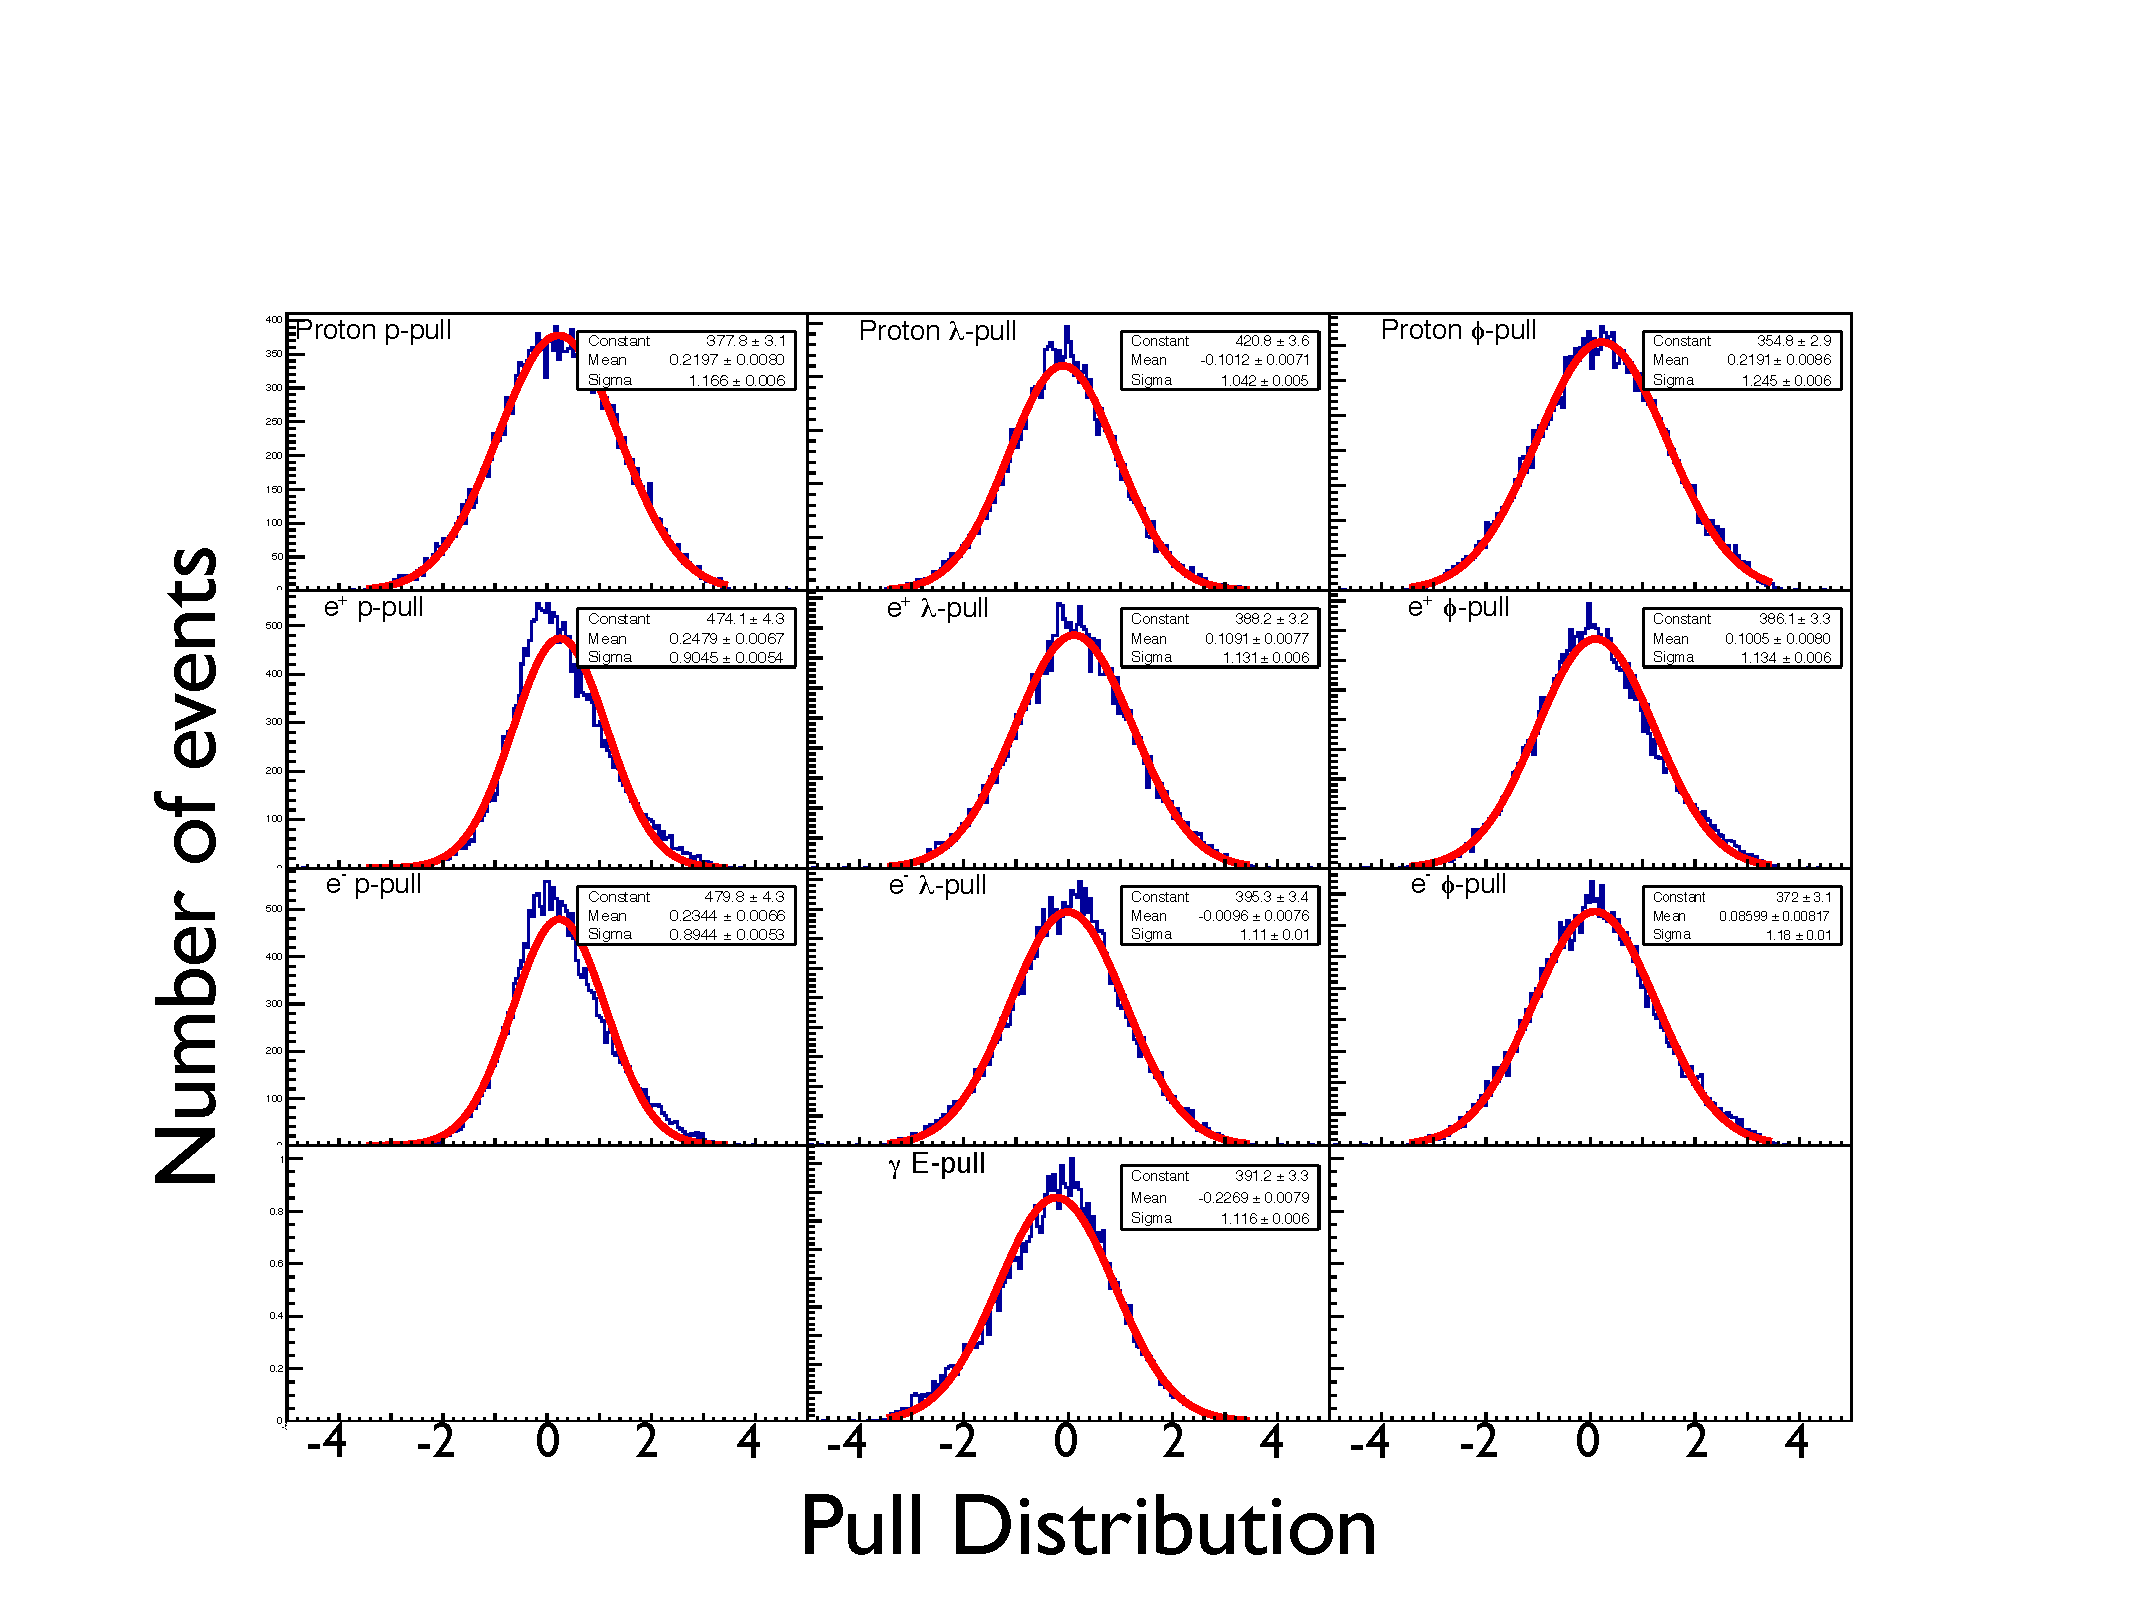
\includegraphics[width=1.2 \figwidth,height= 1.25 \hfigheight]{\figures/analysis/KineFitter/Lep_Pulls_fixII.pdf}
\caption[Number of events vs. Pull distribution for the (4-C) kinematic fit for $\gamma p \rightarrow p e^+ e^-$ for \g12 data with a 1\% Confidence Level cut applied, and a Gaussian fit to each]{\label{fig:kinfit.LepPullData}Number of events vs. Pull distribution for the (4-C) kinematic fit for $\gamma p \rightarrow p e^+ e^-$ for \g12 data with a 1\% Confidence Level cut applied, and a Gaussian fit to each.}
\end{center}\end{figure}
%
%
\begin{figure}[h!]\begin{center}
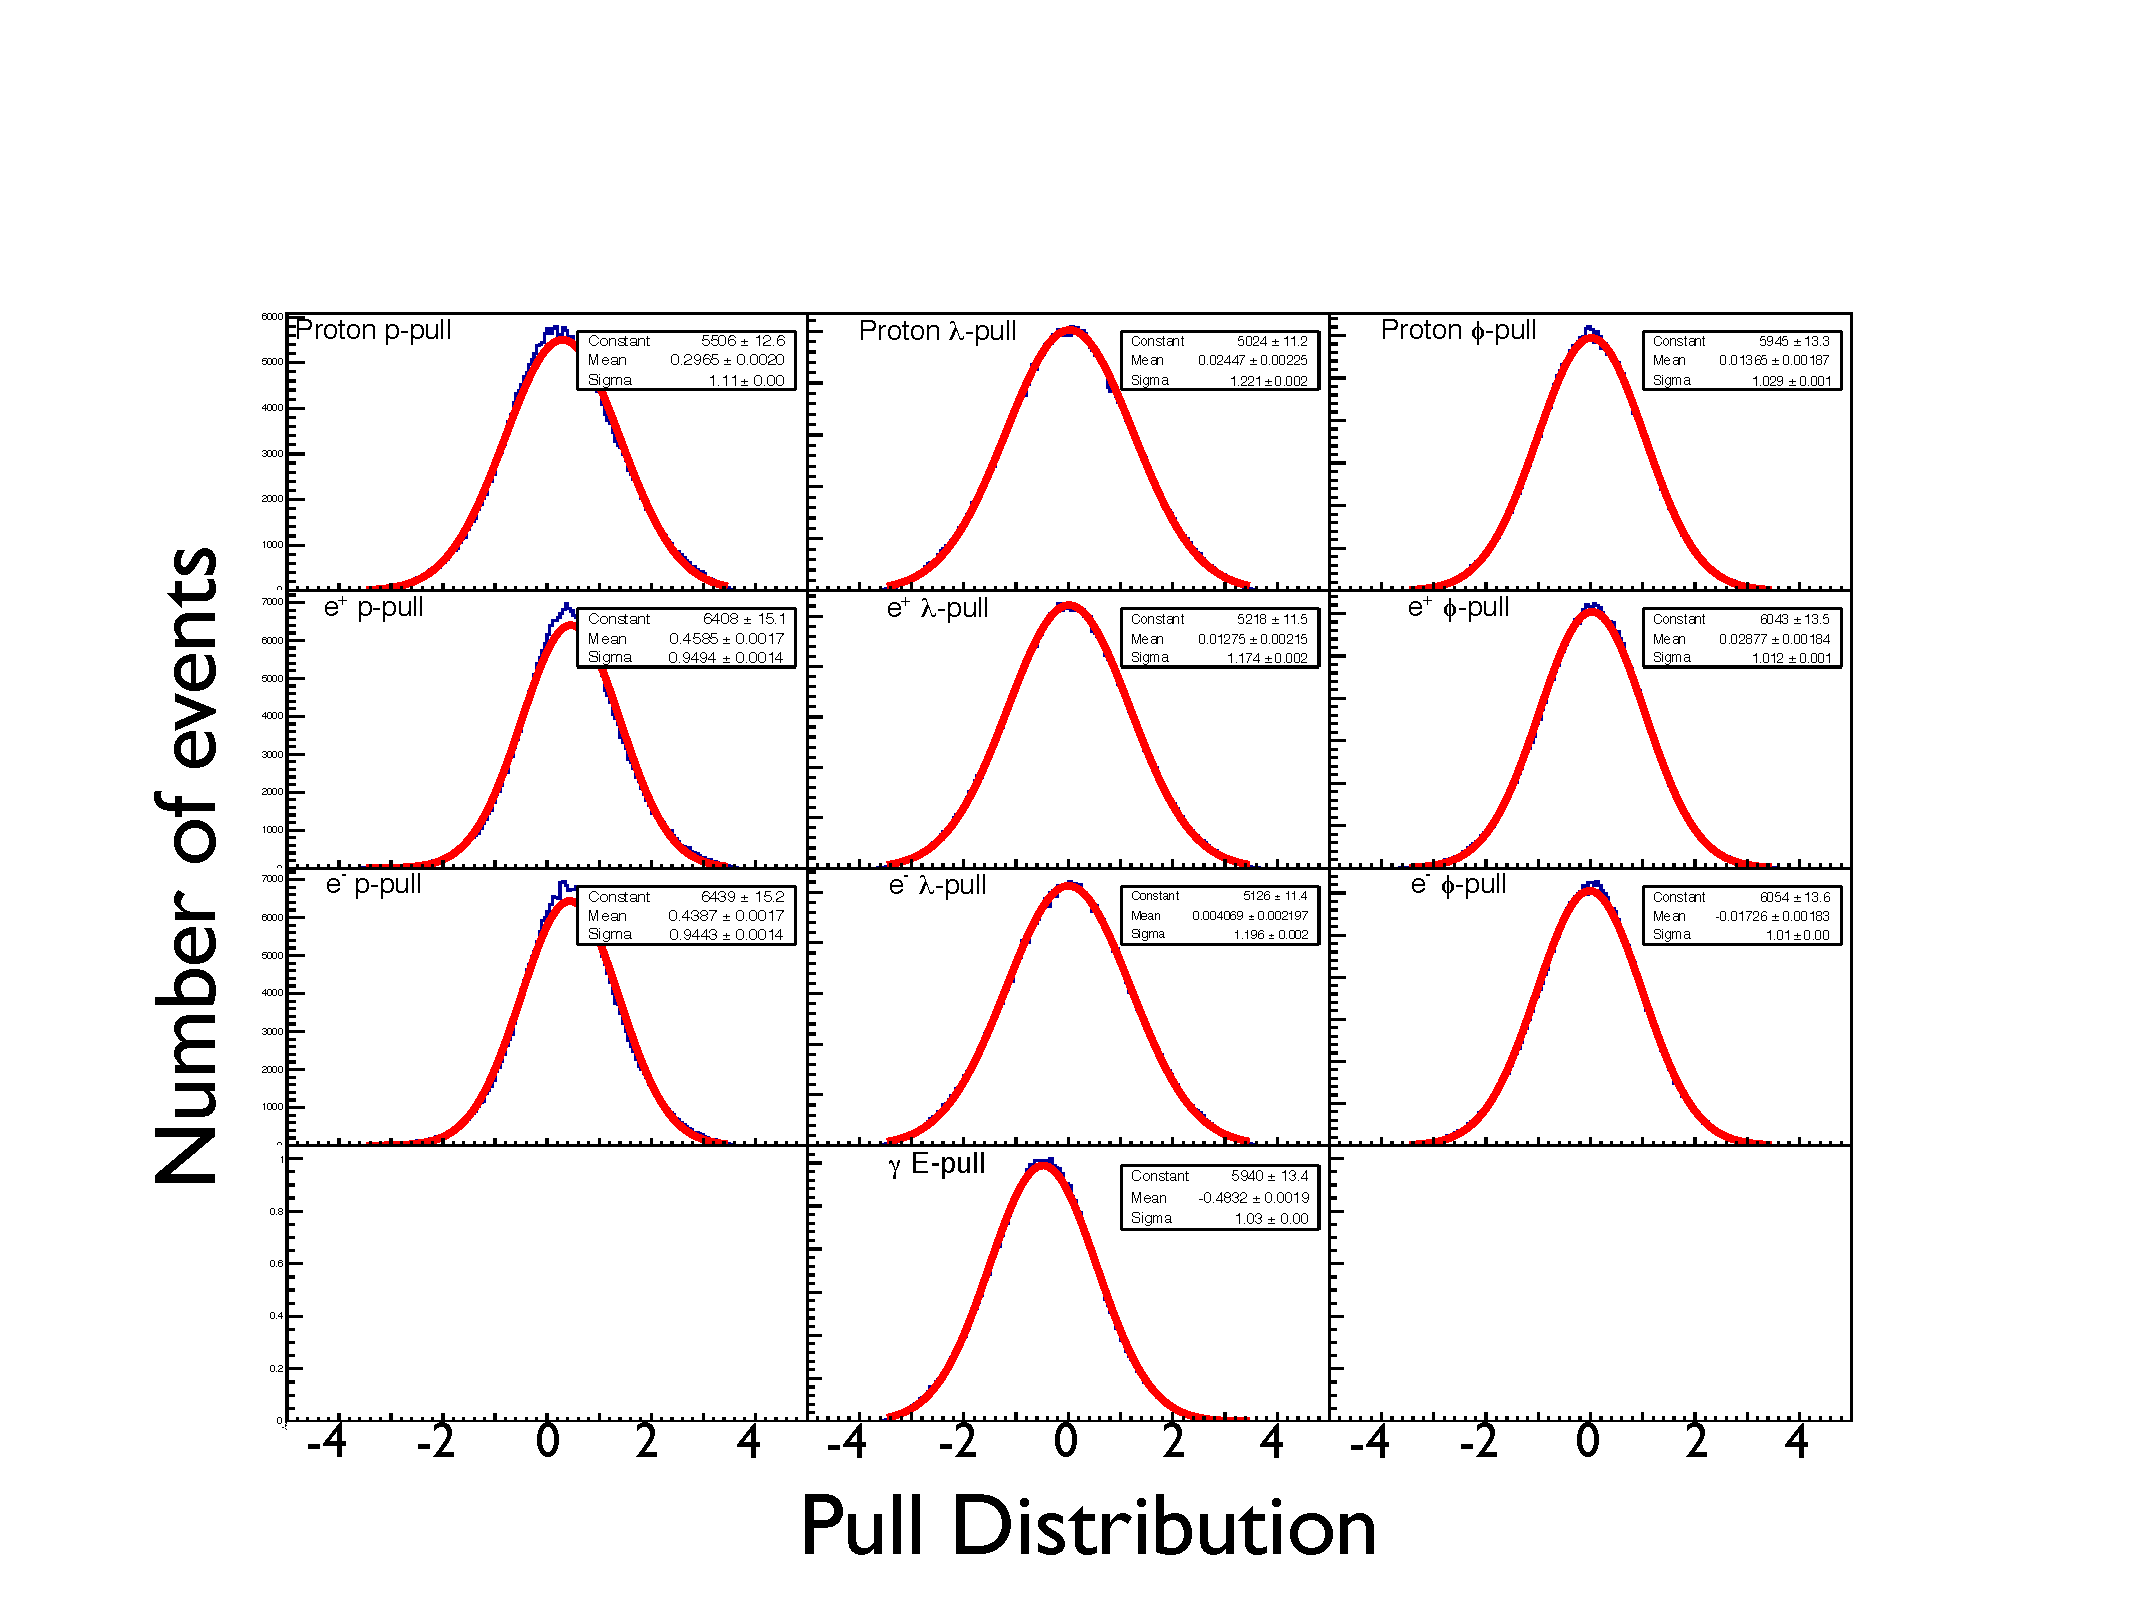
\includegraphics[width=1.2 \figwidth,height= 1.25 \hfigheight]{\figures/analysis/KineFitter/Lep_Pulls_MCII.pdf}
\caption[Number of events vs. Pull distribution for the (4-C) kinematic fit for $\gamma p \rightarrow p e^+ e^-$ for \g12 simulation with a 1\% Confidence Level cut applied, and a Gaussian fit to each]{\label{fig:kinfit.LepPullMC}Number of events vs. Pull distribution for the (4-C) kinematic fit for $\gamma p \rightarrow p e^+ e^-$ for \g12 simulation with a 1\% Confidence Level cut applied, and a Gaussian fit to each.}
\end{center}\end{figure}
%
%
\begin{figure}[h!]\begin{center}
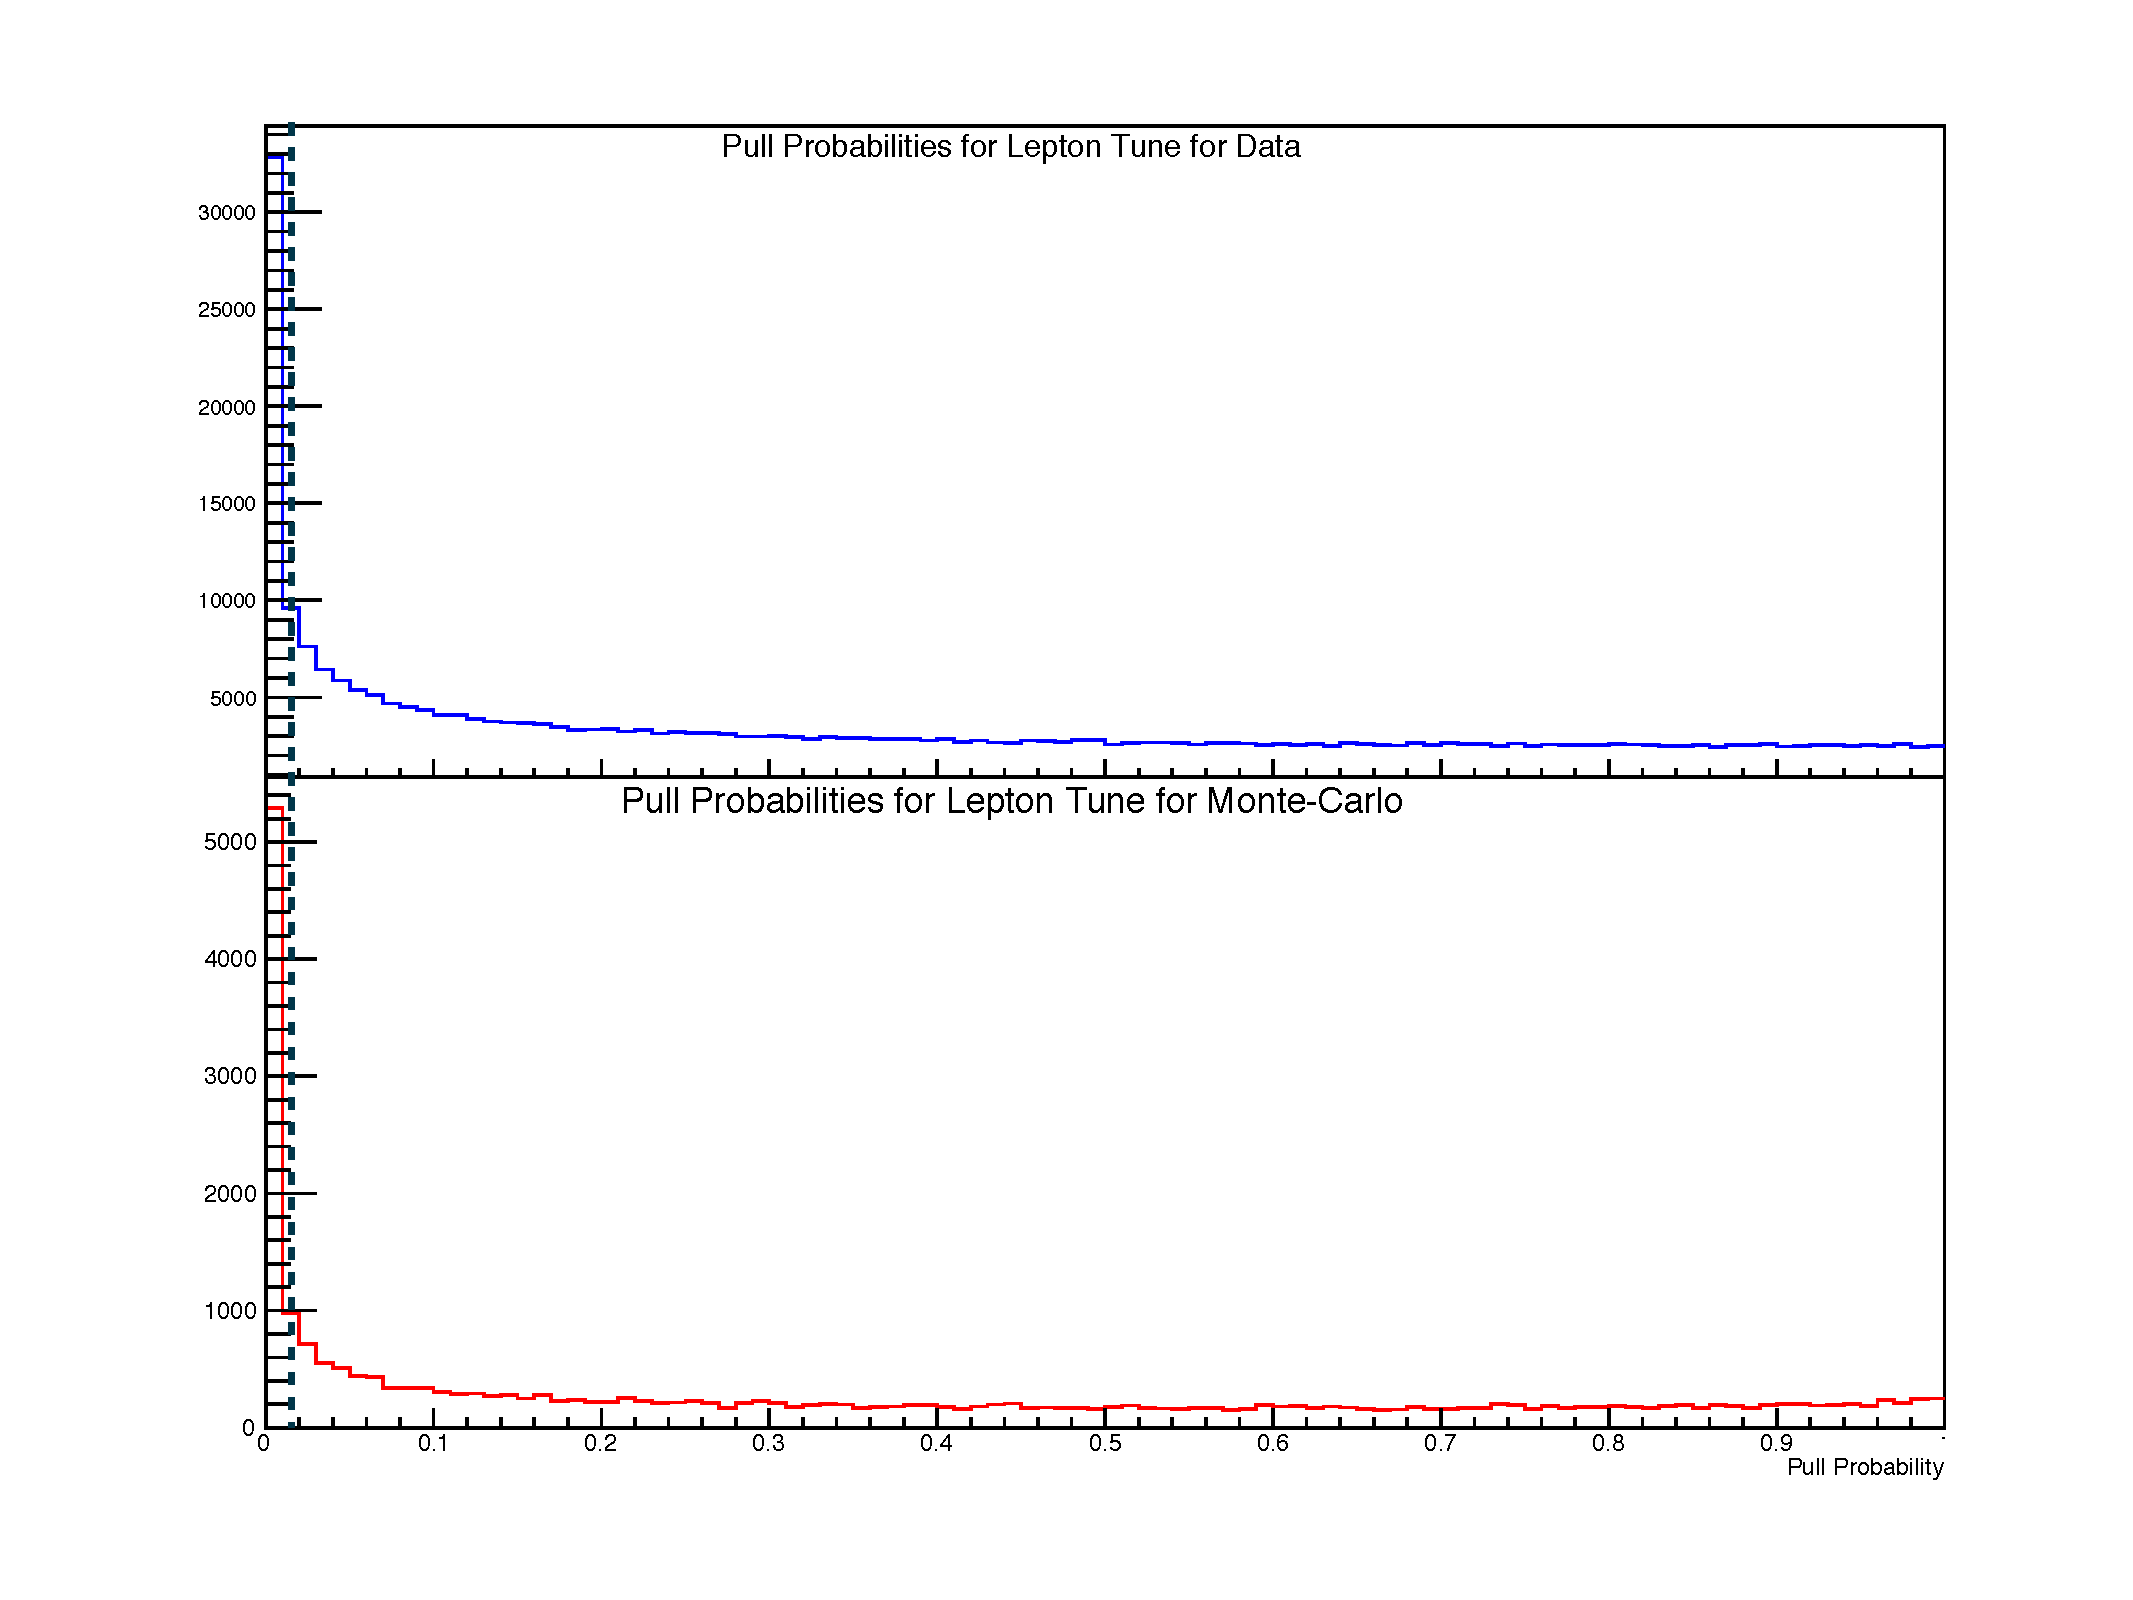
\includegraphics[width=\figwidth,height=  \hfigheight]{\figures/analysis/KineFitter/GP_PEpEm_PullProbThesisII.pdf}
\caption[Number of events vs. Confidence Level for \g12 (top) data and \g12 simulation (bottom) for a (4-C) fit using $\gamma p \rightarrow p e^+ e^-$]{\label{fig:kinfit.LepPullProb}Number of events vs. Confidence Level for \g12 (top) data and \g12 simulation (bottom) for a (4-C) fit using $\gamma p \rightarrow p e^+ e^-$. The black dashed line indicates the cut taken, events with probability $<$1\% are rejected.}
\end{center}\end{figure}
%
\begin{figure}[h!]\begin{center}
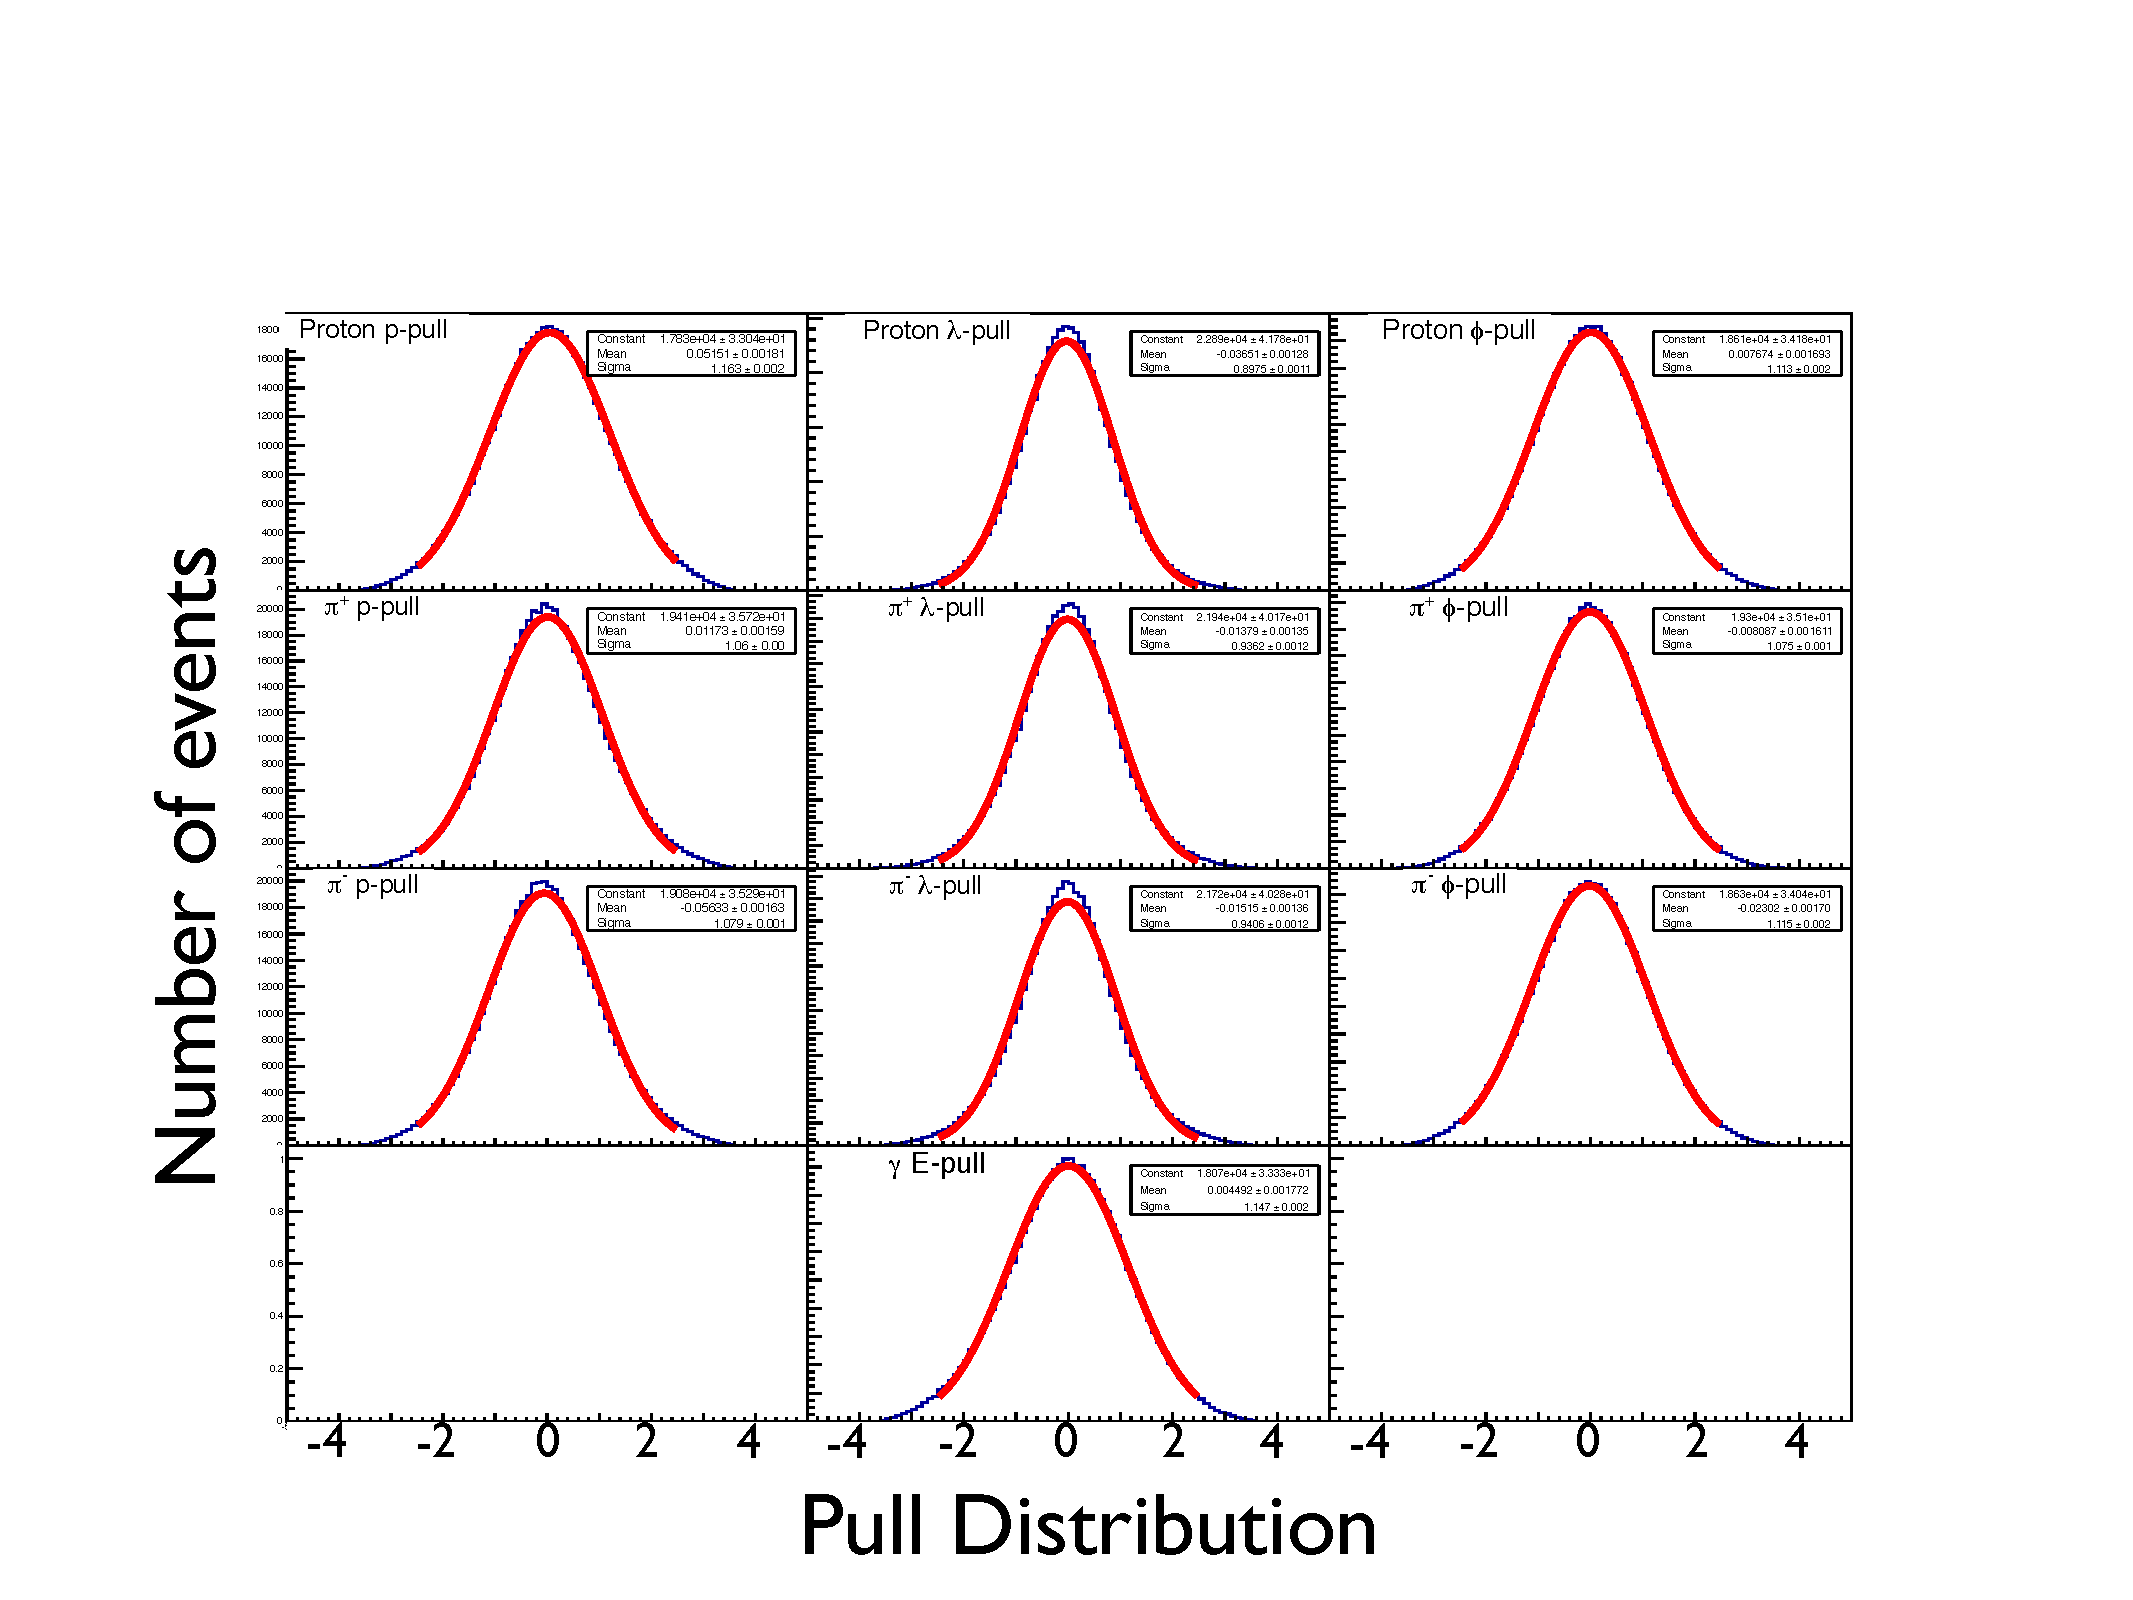
\includegraphics[width=1.2 \figwidth,height= 1.25 \hfigheight]{\figures/analysis/KineFitter/GP_PPipPim_PullsThesisII.pdf}
\caption[Number of events vs. Pull distribution for the (4-C) kinematic fit for $\gamma p \rightarrow p \pi^+ \pi^-$ for \g12 data with a 1\% Confidence Level cut applied, and a Gaussian fit to each]{\label{fig:kinfit.PiPullData}Number of events vs. Pull distribution for the (4-C) kinematic fit for $\gamma p \rightarrow p \pi^+ \pi^-$ for \g12 data with a 1\% Confidence Level cut applied, and a Gaussian fit to each.}
\end{center}\end{figure}
%
%
\begin{figure}[h!]\begin{center}
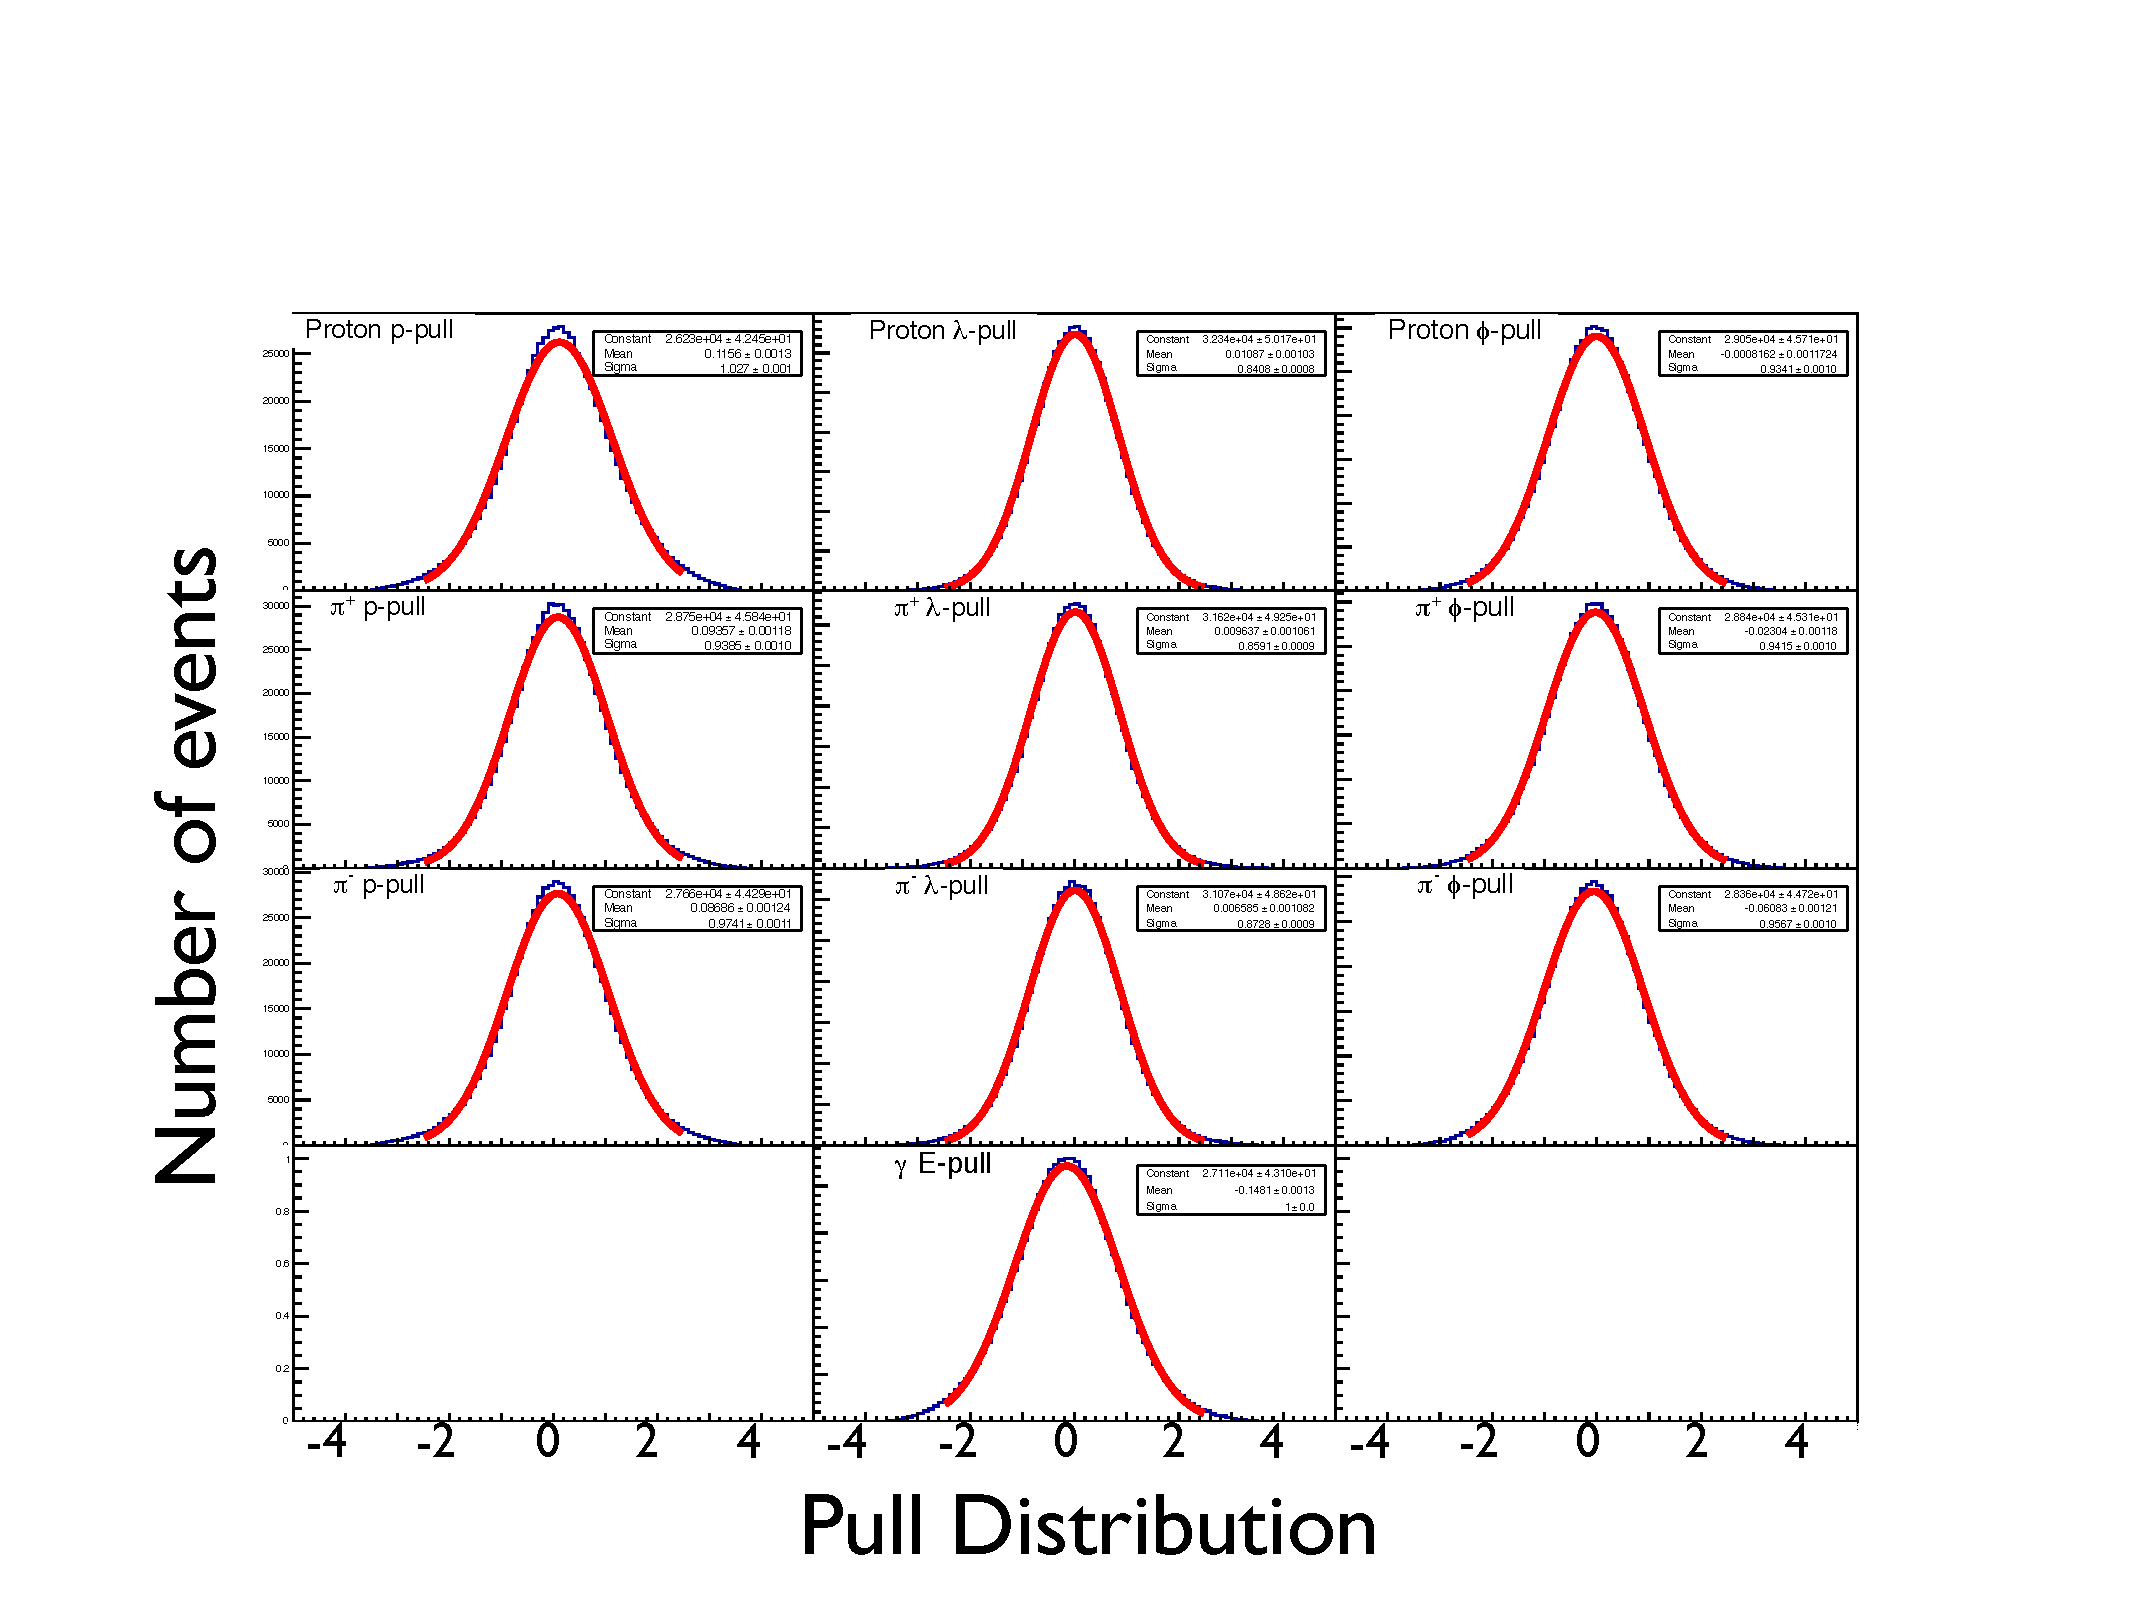
\includegraphics[width=1.2 \figwidth,height= 1.25 \hfigheight]{\figures/analysis/KineFitter/GP_PPipPim_PullsThesis_MCII.pdf}
\caption[Number of events vs. Pull distribution for the (4-C) kinematic fit for $\gamma p \rightarrow p \pi^+ \pi^-$ for \g12 simulation with a 1\% Confidence Level cut applied, and a Gaussian fit to each]{\label{fig:kinfit.PiPullMC}Number of events vs. Pull distribution for the (4-C) kinematic fit for $\gamma p \rightarrow p \pi^+ \pi^-$ for \g12 simulation with a 1\% Confidence Level cut applied, and a Gaussian fit to each.}
\end{center}\end{figure}
%
%
\begin{figure}[h!]\begin{center}
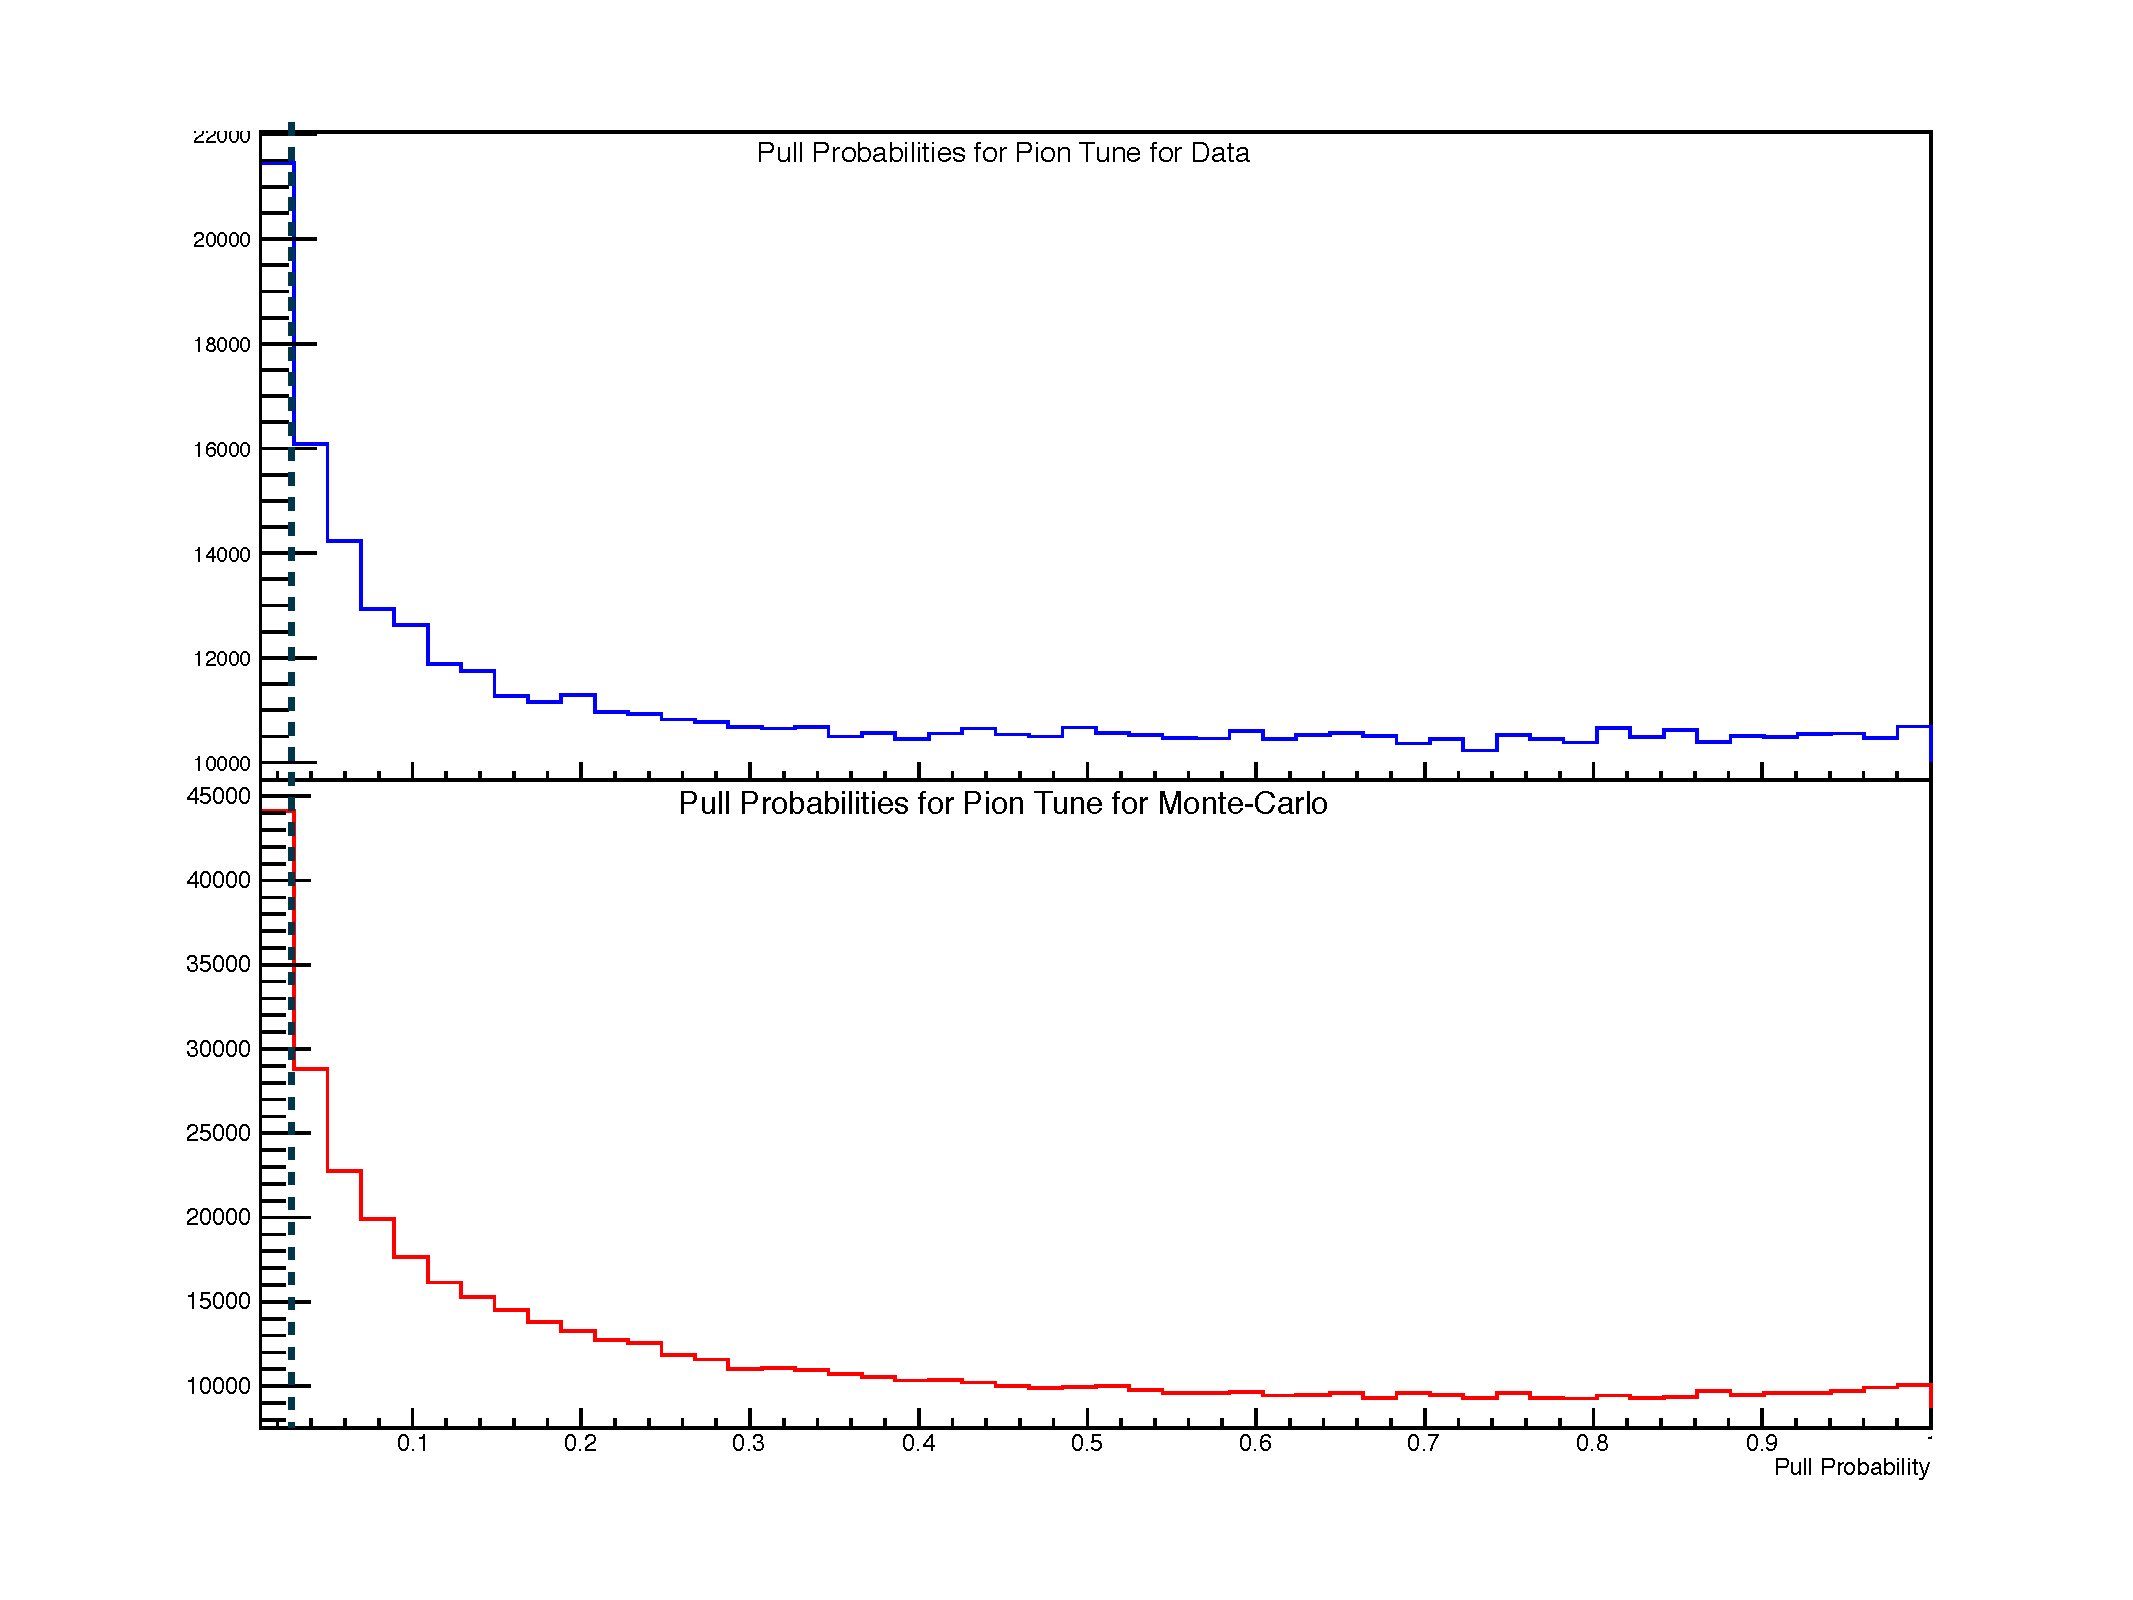
\includegraphics[width=\figwidth,height=  \hfigheight]{\figures/analysis/KineFitter/GP_PPipPim_PullProbThesisII.pdf}
\caption[Number of events vs. Confidence Level for \g12 (top) data and \g12 simulation (bottom) for a (4-C) fit using $\gamma p \rightarrow p \pi^+ \pi^-$]{\label{fig:kinfit.PiPullProb}Number of events vs. Confidence Level for \g12 (top) data and \g12 simulation (bottom) for a (4-C) fit using $\gamma p \rightarrow p \pi^+ \pi^-$. The black dashed line indicates the cut taken, events with probability $<$1\% are rejected.}
\end{center}\end{figure}
%
%
\FloatBarrier
\subsection{Analysis Fitting}\label{sec:analysis.fitting.topology}
This analysis performed three separate kinematic fitting hypotheses, 4-C, 1-C and 2-C. The 4-C fit used the $\gamma p \to p \pi^+ \pi^-$ channel to filter background from double charged pion production from single \piz production. The 1-C fit was used to the topology of $\gamma p \rightarrow p e^+e^-(\gamma)$ to fit to a missing final state photon. The constraint equation for this 1-C fit is given in Eq.~\ref{eq:fit.1C}.
\begin{align}\label{eq:fit.1C}
\mathcal{F} =\left[\begin{array}{c}
E_{beam}+M_p-(E_p+E_{e^+} + E_{e^-} + E_{x}) \\[3pt]
\vec{p}_{beam} - (\vec{p}_{p} +\vec{p}_{e^+} + \vec{p}_{e^-} + \vec{p}_{x})
\end{array}\right]=\vec{0}
\end{align}
The constraint equation for this 4-C fit is given in Eq.~\ref{eq:fit.4C}.
\begin{align}\label{eq:fit.4C}
\mathcal{F} =\left[\begin{array}{c}
E_{beam}+M_p-(E_p+E_{\pi^+} + E_{\pi^-}) \\[3pt]
\vec{p}_{beam} - (\vec{p}_{p} +\vec{p}_{\pi^+} + \vec{p}_{\pi^-})
\end{array}\right]=\vec{0}
\end{align}
The 2-C fit was used to the topology of $\gamma p \rightarrow p e^+e^-(\gamma)$ to fit to a missing final state photon but also to constrain the invariant mass of $e^+e^-(\gamma) = m_{\pi^0}^2$. The constraint equation for this 2-C fit is given in Eq.~\ref{eq:fit.2C}.
\begin{align}\label{eq:fit.2C}
\mathcal{F} =\left[\begin{array}{c}
(E_{e^+} + E_{e^-} + E_{x})^2 - (\vec{p}_{e^+} + \vec{p}_{e^-} + \vec{p}_{x})^2 - M_{\pi^0}^2 \\[3pt]
E_{beam}+M_p-(E_p+E_{e^+} + E_{e^-} + E_{x}) \\[3pt]
\vec{p}_{beam} - (\vec{p}_{p} +\vec{p}_{e^+} + \vec{p}_{e^-} + \vec{p}_{x})
\end{array}\right]=\vec{0}
\end{align}
The ``confidence levels'' for each constraint Eq.~\ref{eq:fit.1C}, ~\ref{eq:fit.4C}, ~\ref{eq:fit.2C} are shown in Fig.~\ref{fig:kinfit.analysispulls} and Fig.~\ref{fig:kinfit.analysispulls_MC} for \g12 data and simulation respectively. These quantities ensure proper mass and energy constraints for this analysis. Cuts on these quantities are discussed in Sec.~\ref{sec:analysis.fitting.compare}. The sparseness of the 4-C fit for simulation is due because background was not simulated for the analysis for reasons discussed in Sec.~\ref{sec:analysis.data.reduction}.
\begin{figure}[h!]\begin{center}
\includegraphics[width=\figwidth,height= 0.75 \hfigheight]{\figures/analysis/KineFitter/LEP_FIT/All_Pulls_uncutII.pdf}
\caption[Number of data events plotted vs. Pull distribution for the 1-C(red), 4-C(black), 2-C(blue) for \g12 data]{\label{fig:kinfit.analysispulls}Number of data events plotted vs. Pull distribution for the 1-C(red,Eq.~\ref{eq:fit.1C}), 4-C(black,Eq.~\ref{eq:fit.4C}), 2-C(blue,Eq.~\ref{eq:fit.2C}) for \g12 data. The orange dashed line illustrates the 1\% cut for all pull distributions.}
\end{center}\end{figure}

\begin{figure}[h!]\begin{center}
\includegraphics[width=\figwidth,height= 0.75 \hfigheight]{\figures/analysis/KineFitter/LEP_FIT/MC/All_Pulls_uncutII.pdf}
\caption[Number of data events plotted vs. Pull distribution for the 1-C(red), 4-C(black), 2-C(blue) for \g12 simulation]{\label{fig:kinfit.analysispulls_MC}Number of data events plotted vs. Pull distribution for the 1-C(red,Eq.~\ref{eq:fit.1C}), 4-C(black,Eq.~\ref{eq:fit.4C}), 2-C(blue,Eq.~\ref{eq:fit.2C}) for \g12 simulation. The orange dashed line illustrates the 1\% cut for all pull distributions.}
\end{center}\end{figure}
\FloatBarrier
%
%
%
\subsection{Kinematic Fitting Analysis and Cuts}\label{sec:analysis.fitting.compare}

The base hypothesis of all corrections performed to the data by the kinematic fitter was the 1-C constraint equation found in Eq.~\ref{eq:fit.1C}. This means that all fitted data will be presented in quantities based upon the hypothesis of a missing photon. The effect of 1-C kinematic fitting for events, prior to any topological cuts, with beam energies less than 3.6~GeV can be seen in Fig.~\ref{fig:kinfit.effect_lep}, while for beam energies greater than 3.6~GeV can be seen in Fig.~\ref{fig:kinfit.effect_mor}. The top panel depicts the unfitted data and the bottom panel depicts the data output from the kinematic fitter. The red data line represents all data while the blue line depicts the data where cuts were placed on \abbr{CC} and \abbr{EC} hits in order to satisfy the trigger as discussed in Sec~\ref{sec.data.trig.lepton}. The red, vertical dashed-dotted line illustrates the production point for two charged pion production. The \abbr{MC} counterpart plots of Figs.~\ref{fig:kinfit.effect_lep}, ~\ref{fig:kinfit.effect_mor} can be seen in Figs.~\ref{fig:kinfit.effect_lepMC}, ~\ref{fig:kinfit.effect_morMC}, where only the \piz signal was simulated.

It can be seen that the effects of the 1-C fit, prior to topological cuts, narrows the \piz signal for events with beam energies less than 3.6~GeV, while for energies greater than 3.6~GeV, the 1-C fit reveals a signal that appears hidden without further cuts for the data.
\begin{figure}[h!]\begin{center}
\includegraphics[width=\figwidth,height= 0.75 \hfigheight]{\figures/analysis/KineFitter/DATA/mm2P_compare_leptrig.pdf}
\caption[Number of data events plotted vs. missing mass $M_x(\gamma p \to p X)$ for uncut data and $E_\gamma < 3.6$~GeV]{\label{fig:kinfit.effect_lep}Number of data events plotted vs. missing mass $M_x(\gamma p \to p X)$ for uncut data and $E_\gamma < 3.6$~GeV. The top panel depicts the unfitted data, where the red data line represents all data while the blue line depicts all data with cuts placed on \abbr{CC} and \abbr{EC}. The bottom panel depicts the data output from the kinematic fitter 1-C fit, where the red data line represents all data while the blue line depicts all data with cuts placed on \abbr{CC} and \abbr{EC}.  }
\end{center}\end{figure}

\begin{figure}[h!]\begin{center}
\includegraphics[width=\figwidth,height= 0.75 \hfigheight]{\figures/analysis/KineFitter/DATA/mm2P_compare_mortrig.pdf}
\caption[Number of data events plotted vs. missing mass $M_x(\gamma p \to p X)$ for uncut data and $E_\gamma > 3.6$~GeV]{\label{fig:kinfit.effect_mor}Number of data events plotted vs. missing mass $M_x(\gamma p \to p X)$ for uncut data and $E_\gamma > 3.6$~GeV. The top panel depicts the unfitted data. The bottom panel depicts the data output from the kinematic fitter 1-C fit.}
\end{center}\end{figure}

\begin{figure}[h!]\begin{center}
\includegraphics[width=\figwidth,height= 0.75 \hfigheight]{\figures/analysis/KineFitter/MC/mm2P_compare_leptrig.pdf}
\caption[Number of \abbr{MC} events plotted vs. missing mass $M_x(\gamma p \to p X)$ for uncut data and $E_\gamma < 3.6$~GeV]{\label{fig:kinfit.effect_lepMC}Number of \abbr{MC} events plotted vs. missing mass $M_x(\gamma p \to p X)$ for uncut data and $E_\gamma < 3.6$~GeV. The top panel depicts the unfitted data, where the red data line represents all data while the blue line depicts all data with cuts placed on \abbr{CC} and \abbr{EC} hits to be present. The bottom panel depicts the data output from the kinematic fitter 1-C fit, where the red data line represents all data while the blue line depicts all data with cuts placed on \abbr{CC} and \abbr{EC} hits to be present.  }
\end{center}\end{figure}

\begin{figure}[h!]\begin{center}
\includegraphics[width=\figwidth,height= 0.75 \hfigheight]{\figures/analysis/KineFitter/MC/mm2P_compare_mortrig.pdf}
\caption[Number of \abbr{MC} events plotted vs. missing mass $M_x(\gamma p \to p X)$ for uncut data and $E_\gamma > 3.6$~GeV]{\label{fig:kinfit.effect_morMC}Number of \abbr{MC} events plotted vs. missing mass $M_x(\gamma p \to p X)$ for uncut data and $E_\gamma > 3.6$~GeV. The top panel depicts the unfitted data. The bottom panel depicts the data output from the kinematic fitter 1-C fit.}
\end{center}\end{figure}
\FloatBarrier

\subsubsection{1-C \& 4-C Cuts}
As mentioned in Sec~\ref{sec:analysis.fitting.topology}, there were 3 constraint equations used in this analysis. The 1-C fit utilizes a constraint equation to a missing photon, while the 4-C fit assumed a $\pi^+\pi^-$ topology instead of the \epem topology. In this analysis a $>$1\% confidence level cut was placed on the 1-C fit to ensure the missing photon is in the event. However, a $<$1\% confidence level cut was placed on the 4-C fit to remove the $\pi^+\pi^-$ background. The effect of the pull distributions after placing these cuts can be seen in Fig.~\ref{fig:kinefit.pull.Data.MC}. The effect of the 1-C and 4-C cut on the data can be seen in Fig.~\ref{kinefit.Mass.Data.MC}, where the blue line depicts the uncut fitted data spectrum, except the trigger cut, the black line depicts after a $>$1\% cut placed on the 1-C and green line depicts the effect of the $<$1\% 4-C fit cut. Top panel illustrates the effect of the cuts on recorded data, bottom panel illustrates the effect of the cuts on \abbr{MC}. The top plot of each panel depicts events of beam energies less than 3.6~GeV, while the bottom plot of each panel depicts events of beam energies greater than 3.6~GeV. It is shown in Fig.~\ref{fig:kinefit.pulleffect.data} that each cut depletes the background while maintaining signal.


\begin{figure}[h!]\begin{center}
\subfloat[Analysis Pull Distributions After Pull Selection for Data][]{ %Feynman diagram of \piz two photon decay
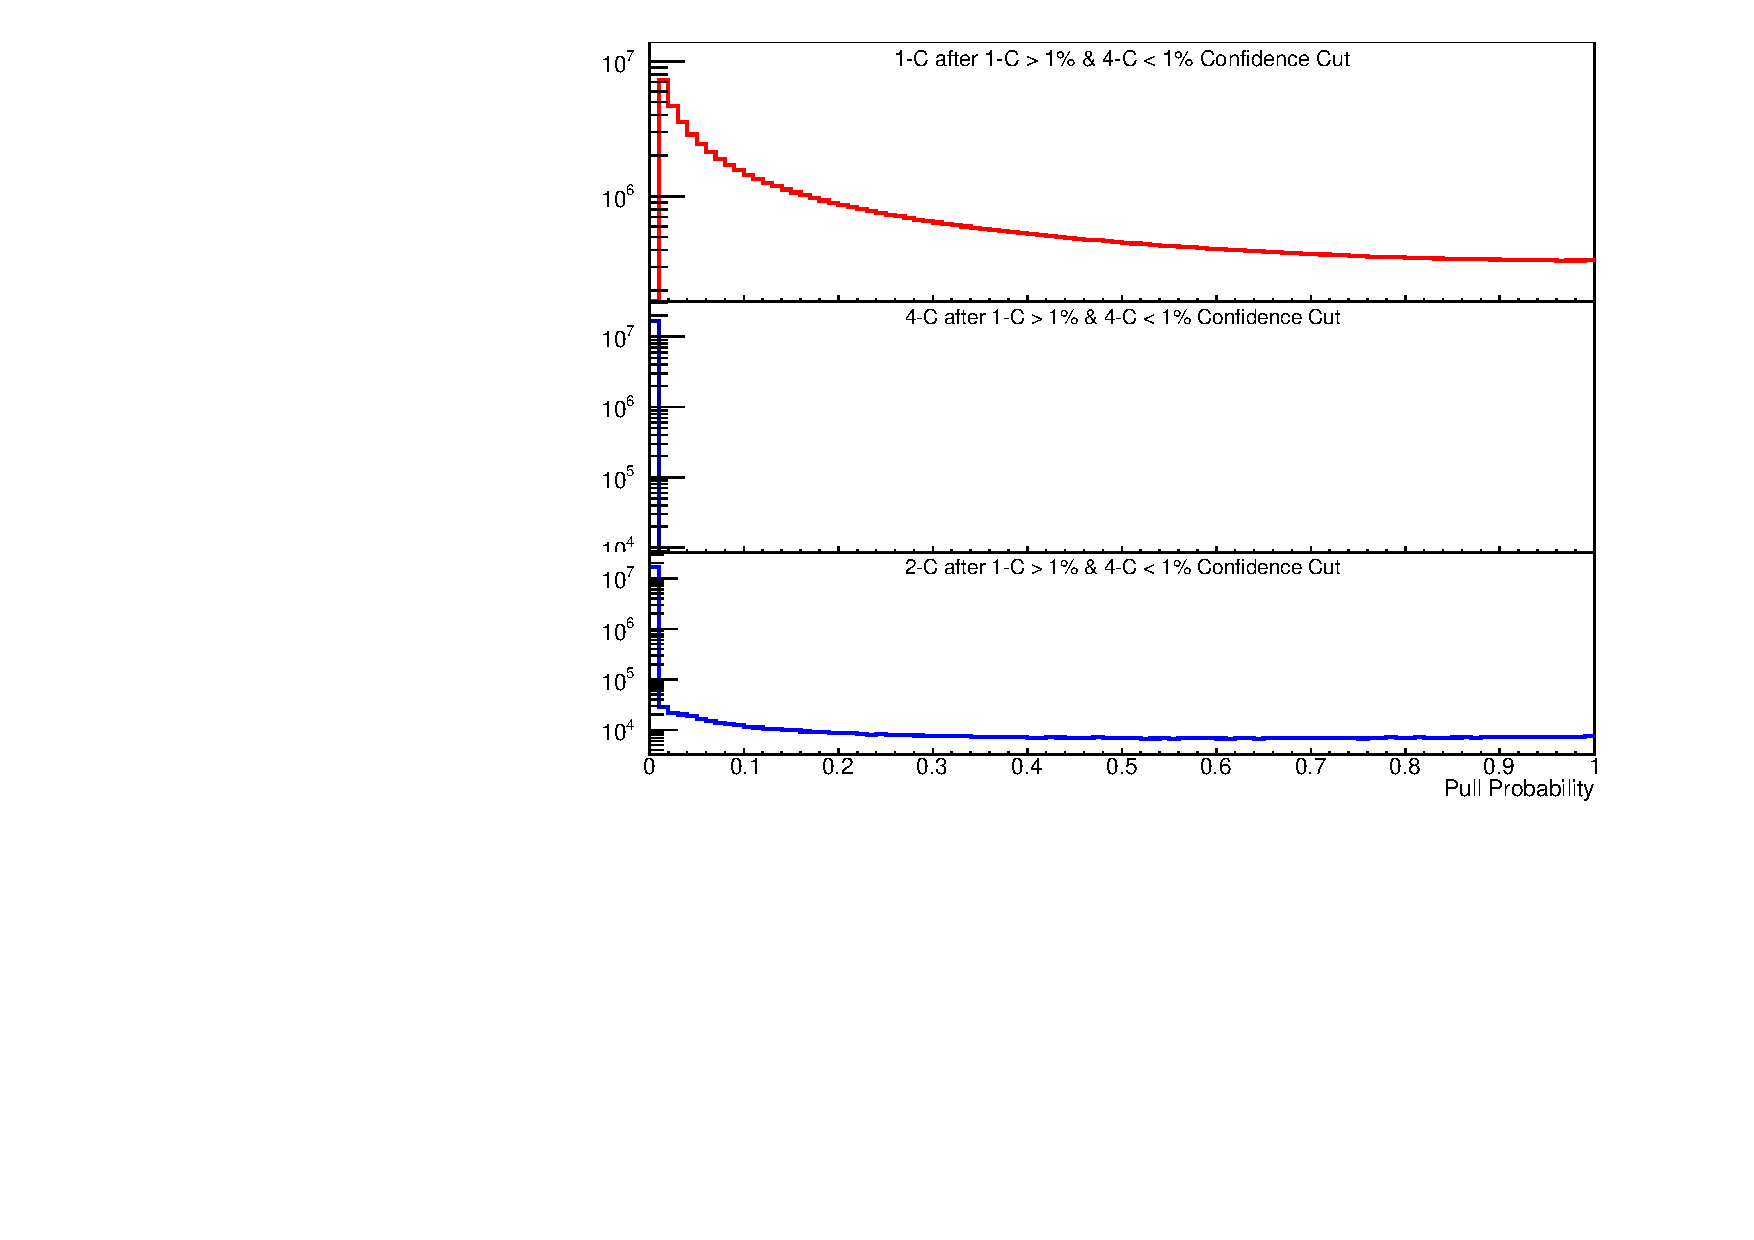
\includegraphics[width=0.8\columnwidth,height=\qfigheight]{\figures/analysis/KineFitter/DATA/All_Pulls_picut.pdf}\label{fig:kinefit.pulldata}
}

\subfloat[Analysis Pull Distributions After Pull Selection for \abbr{MC}][]{ %Feynman diagram of \piz Dalitz decay
\includegraphics[width=0.8\columnwidth,height=\qfigheight]{\figures/analysis/KineFitter/MC/All_Pulls_picut.pdf}\label{fig:kinefit.pullMC}
}
\caption[Number of events vs. Pull distributions after a 1\% cut placed on the 1-C (top plots) and 4-C fit (middle plots) for data and \abbr{MC}]{\label{fig:kinefit.pull.Data.MC}Number of events vs. Pull distributions after a 1\% cut placed on the 1-C (top plots) and 4-C fit (middle plots) for data~\subref{fig:kinefit.pulldata} and \abbr{MC}~\subref{fig:kinefit.pullMC}.}

\end{center}\end{figure}


\begin{figure}[h!]\begin{center}
\subfloat[Mass Distributions After Pull Selection for Data][]{ %Feynman diagram of \piz two photon decay
\includegraphics[width=0.8\columnwidth,height=\qfigheight]{\figures/analysis/KineFitter/DATA/mm2P_w_Pull_cuts.pdf}\label{fig:kinefit.pulleffect.data}
}

\subfloat[Mass Distributions After Pull Selection for \abbr{MC}][]{ %Feynman diagram of \piz Dalitz decay
\includegraphics[width=0.8\columnwidth,height=\qfigheight]{\figures/analysis/KineFitter/MC/mm2P_w_Pull_cuts.pdf}\label{fig:kinefit.pulleffect.MC}
}
\caption[Number of data events plotted vs. missing mass $M_x(\gamma p \to p X)$]{\label{kinefit.Mass.Data.MC}Number of data events plotted vs. missing mass $M_x(\gamma p \to p X)$. Blue lines depict the fitted data prior to pull distribution cuts, black line depicts after a 1\% cut placed on the 1-C and green line depicts the effect of the 1\% 4-C fit cut. Top panel~\subref{fig:kinefit.pulldata} depicts data while bottom panel~\subref{fig:kinefit.pulleffect.MC} depicts \abbr{MC}.}

\end{center}\end{figure}
\FloatBarrier
\subsubsection{Missing Energy  Cut}
The remainder of the background can be attributed to $\pi^+\pi^-$ events. To reduce the background further, a comparison of the missing mass squared off of the proton and the missing energy of the system was performed. This comparison is plotted in Fig.~\ref{kinefit.mm2p.mE.data.MC}, where it can seen that the majority of $\pi^+\pi^-$ background has missing energy less than 75~MeV. To eliminate this background all events with a missing energy less than ~75~MeV were cut out.
\begin{figure}[h!]\begin{center}
\subfloat[$\mathrm{M_x^2(p)}$ vs. $\mathrm{M_E^2(pe^+e^-)}$ for Data][]{ %Feynman diagram of \piz two photon decay
\includegraphics[width=0.8\columnwidth,height=0.75 \hfigheight]{\figures/analysis/KineFitter/DATA/mm2P_vs_mEPEpEm.pdf}\label{fig:kinefit.mm2p.mE.data}
}

\subfloat[$\mathrm{M_x^2(\gamma p \to p X)}$ vs. $\mathrm{M_E^2(\gamma p \to pe^+e^- X)}$ for \abbr{MC}][]{ %Feynman diagram of \piz Dalitz decay
\includegraphics[width=0.8\columnwidth,height=0.75 \hfigheight]{\figures/analysis/KineFitter/MC/mm2P_vs_mEPEpEm.pdf}\label{fig:kinefit.mm2p.mE.MC}
}
\caption[$\mathrm{M_x^2(\gamma p \to p X)}$ vs. $\mathrm{M_E(\gamma p \to pe^+e^- X)}$]{\label{kinefit.mm2p.mE.data.MC}$\mathrm{M_x^2(\gamma p \to p X)}$ vs. $\mathrm{M_E(\gamma p \to pe^+e^- X)}$. The horizontal red dashed-dotted line depicts the 75~MeV cut used in this analysis. The vertical red dashed-dotted line depicts boundary of single \piz to $\pi^+\pi^-$  production. Top panel depicts data, while the bottom panel depicts \abbr{MC}.}

\end{center}\end{figure}

The effect of the 75~MeV missing energy cut on the $M_x^2(p)$ spectrum can be seen in Fig.~\ref{kinefit.mm2p.data.MC}. The signal function (red solid) is the \emph{Crystal Ball Function}~\cite{CBwiki},~\cite{CBjlab} and the background (black) a $3^{rd}$ order polynomial. The contamination of the background under the \piz signal for data events where the beam energy is less than 3.6~GeV is $1.3~\%$. The contamination of the background under the \piz signal for data events where the beam energy is greater than 3.6~GeV is $2.1~\%$. This background can be reduced more with the 2-C cut. 
The Crystal Ball function, named after the Crystal Ball Collaboration, is a probability density function commonly used to model various lossy processes in high-energy physics. It consists of a Gaussian core portion and a power-law low-end tail, below a certain threshold. The function itself and its first derivative are both continuous~\cite{CBjlab}. 
\begin{align}
f(x;\alpha,n,\bar{x},\sigma)=N\cdot
\begin{cases}
\mathrm{exp}(-\frac{(x-\bar{x})^2}{2 \sigma^2}), & \text{for }\frac{x-\bar{x}}{\sigma}>-\alpha \\
A \cdot (B - \frac{x-\bar{x}}{\sigma})^{-n}, & \text{for }\frac{x-\bar{x}}{\sigma} \le -\alpha
\end{cases}
\end{align}
where
\begin{align}
A = \left( \frac{n}{\left| \alpha \right|}\right)^n \cdot \mathrm{exp} \left( - \frac{\left| \alpha \right|^2}{2}\right) \nonumber  \\
B=\frac{n}{\left| \alpha \right|} - \left| \alpha \right|
\end{align}
N is a normalization factor and $\alpha$, $n$, $x$ and $\sigma$ are parameters which are fitted with the data.
\begin{figure}[h!]\begin{center}
\subfloat[Mass Distributions After Pull \& $\mathrm{M_E^2(pe^+e^-)}$ Selection for Data][]{ %Feynman diagram of \piz two photon decay
\includegraphics[width=0.8\columnwidth,height=0.75 \hfigheight]{\figures/analysis/KineFitter/DATA/hdataLEP_MOR_pi0_Combine.pdf}\label{fig:kinefit.mm2p.data}
}

\subfloat[Mass Distributions After Pull \& $\mathrm{M_E^2(pe^+e^-)}$ Selection for \abbr{MC}][]{ %Feynman diagram of \piz Dalitz decay
\includegraphics[width=0.8\columnwidth,height=0.75 \hfigheight]{\figures/analysis/KineFitter/MC/hdataLEP_MOR_pi0_Combine_MC.pdf}\label{fig:kinefit.mm2p.MC}
}
\caption[Number of data events plotted vs. missing mass $M_x(\gamma p \to p X)$ after the 1-C, 4-C and 75~MeV missing energy cut]{\label{kinefit.mm2p.data.MC}Number of data events plotted vs. missing mass $M_x(\gamma p \to p X)$ after the 1-C, 4-C and 75~MeV missing energy cut. Top plots depicts the data. Bottom plot depicts the \abbr{MC}. For both panels, the top plots illustrate events with beam energies less than 3.6~GeV, while the bottom plot illustrates events with beam energies greater than 3.6~GeV. The red solid line are fits using the \emph{Crystal Ball Function}, while the black line illustrates the $3^{rd}$ order polynomial background function. }

\end{center}\end{figure}
\FloatBarrier
\subsubsection{2-C Cut}
The final cut the was utilized in the analysis was the 2-C constraint. The 2-C constraint fits to a missing final state photon but also constrains the invariant mass of $e^+e^-(\gamma) = m_{\pi^0}^2$. The constraint equation for this 2-C fit is given in Eq.~\ref{eq:fit.2C}. This analysis used a $>1\%$ confidence level cut on the 2-C fit, this translates to a $2.5\sigma$ cut of a Gaussian function if a Gaussian was assumed for the signal instead of the \emph{Crystal Ball Function}. The effect of the 2-C cut after the 1-C, 4-C and missing energy cut on the data can be seen in Fig.~\ref{kinefit.mm2pfinal.data}, where the top plot of each panel illustrates the mass spectrum prior to the $>1\%$ 2-C cut and the bottom plot of each panel illustrates the mass spectrum after to the $>1\%$ 2-C cut along with the other cuts. To show the full effect fo the 2-C fit, the bottom plot of each panel has the fits of their top plots superimposed. For events under 3.6~GeV in beam energy, the 2-C cut has little effect, which is expected because this spectrum presented itself almost background free due to the \abbr{CC} and \abbr{EC} trigger constraints. For events above 3.6~GeV in beam energy, the 2-C cut has greater effect, which is expected because this spectrum presented itself with an irreducible $\pi^+\pi^-$ background. The effect of the 2-C cut on \abbr{MC}, Fig.~\ref{kinefit.mm2pfinal.MC}, is minimal as well due to the \piz spectrum being the only topology simulated. The blue lines atop of the data spectrum for each plot in which the 2-C cuts was taken, shows the new fit using the \emph{Crystal Ball Function}. The mass differences from the accepted value~\cite{pdg2014} to the fitted value are 1.2~MeV and 1.7~MeV for the events below 3.6~GeV and above 3.6~GeV respectively.
%The confidence level cut of 2-C fit can be directly translated as $\pm \sigma$ cuts from standard data manipulation cuts, however with the 2-C fit cut it allows for the tails of the distribution to be accepted.   The visual depiction of the pull distributions after placing the 2-C $>1\%$ cut with also the other 1-C and 4-C and missing energy cuts can be seen in Fig.~\ref{fig:kinefit.pull.Data.MC.all}.
%\begin{figure}[h!]\begin{center}
%\subfloat[All Analysis Pull Distributions for Data][]{ %Feynman diagram of \piz two photon decay
%\includegraphics[width=0.8\columnwidth,height=\qfigheight]{\figures/analysis/KineFitter/DATA/All_Pulls_allcuts.pdf}\label{fig:kinefit.pulldata.all}
%}
%
%\subfloat[All Analysis Pull Distributions for \abbr{MC}][]{ %Feynman diagram of \piz Dalitz decay
%\includegraphics[width=0.8\columnwidth,height=\qfigheight]{\figures/analysis/KineFitter/MC/All_Pulls_allcuts.pdf}\label{fig:kinefit.pullMC.all}
%}
%\caption[Analysis Pull Distributions After Pull Selection]{\label{fig:kinefit.pull.Data.MC.all}Pull distributions after a 1\% cut placed on the 1-C, 1\% cut on 4-C fit and 1\% on 2-C fit for data~\subref{fig:kinefit.pulldata.all} and \abbr{MC}~\subref{fig:kinefit.pullMC.all}.}
%
%\end{center}\end{figure}

\begin{figure}[h!]\begin{center}
\subfloat[Mass Distributions After All Confidence Level and Missing Energy Cuts for Data E$_{beam} < 3.6$~GeV][]{ %Feynman diagram of \piz two photon decay
\includegraphics[width=0.8\columnwidth,height=0.75 \hfigheight]{\figures/analysis/KineFitter/DATA/hdataLEP_pi0_Combine.pdf}\label{fig:kinefit.mm2pfinalLEP.data}
}

\subfloat[Mass Distributions After All Confidence Level and Missing Energy Cuts for Data E$_{beam} > 3.6$~GeV][]{ %Feynman diagram of \piz Dalitz decay
\includegraphics[width=0.8\columnwidth,height=0.75 \hfigheight]{\figures/analysis/KineFitter/DATA/hdataMOR_pi0_Combine.pdf}\label{fig:kinefit.mm2pfinalMOR.data}
}
\caption[Number of data events plotted vs. missing mass $M_x(\gamma p \to p X)$ after the 1-C, 4-C, 2-C and 75~MeV missing energy cut]{\label{kinefit.mm2pfinal.data}Number of data events plotted vs. missing mass $M_x(\gamma p \to p X)$ after the 1-C, 4-C and 75~MeV missing energy cut. For both panels, the top plots illustrates events with beam energies less than 3.6~GeV, while the bottom plot illustrates events with beam energies greater than 3.6~GeV. The red solid line are fits using the \emph{Crystal Ball Function}, while the black line illustrates the $3^{rd}$ order polynomial background function. The bottom plot on the bottom panel shows what the background and signal function parameters were without the 2-C cut for comparison.}
\end{center}\end{figure}



\begin{figure}[h!]\begin{center}
\subfloat[Mass Distributions After All Confidence Level and Missing Energy Cuts for \abbr{MC} E$_{beam} < 3.6$~GeV][]{ %Feynman diagram of \piz two photon decay
\includegraphics[width=0.8\columnwidth,height=0.75 \hfigheight]{\figures/analysis/KineFitter/MC/hdataLEP_pi0_Combine_MC.pdf}\label{fig:kinefit.mm2pfinalLEP.MC}
}

\subfloat[Mass Distributions After All Confidence Level and Missing Energy Cuts for \abbr{MC} E$_{beam} > 3.6$~GeV][]{ %Feynman diagram of \piz Dalitz decay
\includegraphics[width=0.8\columnwidth,height=0.75 \hfigheight]{\figures/analysis/KineFitter/MC/hdataMOR_pi0_Combine_MC.pdf}\label{fig:kinefit.mm2pfinalMOR.MC}
}
\caption[Number of \abbr{MC} events plotted vs. missing mass $M_x(\gamma p \to p X)$ after the 1-C, 4-C, 2-C and 75~MeV missing energy cut]{\label{kinefit.mm2pfinal.MC}Number of \abbr{MC} events plotted vs. missing mass $M_x(\gamma p \to p X)$ after the 1-C, 4-C, 2-C and 75~MeV missing energy cut. For both panels, the top plots illustrates events with beam energies less than 3.6~GeV, while the bottom plot illustrates events with beam energies greater than 3.6~GeV. The red solid line are fits using the \emph{Crystal Ball Function}, while the black line illustrates the $3^{rd}$ order polynomial background function. The bottom plot on the bottom panel shows what the background and signal function parameters were without the 2-C cut for comparison.}

\end{center}\end{figure}

\FloatBarrier

\section{Particle Vertex Timing Cuts}\label{sec:analysis.timing}
Another quantity that is used for \abbr{PID} and data cleanliness is the vertex timing $t_{vert}$, which is the time the particle left the target. It can be calculated as;
\begin{align}
t_{vert}= t_{\abbr{TOF}} -  l_{\abbr{TOF}}/(c\beta) \label{eq:tvert.tof}
\end{align}
where $t_{\abbr{TOF}}$ and $l_{\abbr{TOF}}$ are the time and length measurement, respectively, recorded at the \abbr{TOF} subsystem, and $c$ is the speed of light. The value of $\beta$ is calculated using the particles mass, $m$, and momentum, $p$, as measured from the \abbr{DC}. Therefore $\beta = \frac{p}{E} = \frac{p}{\sqrt{p^2+m^2}}$. Another means of calculating $t_{vert}$ is to use the timing of the tagger hit using the RF-corrected tagger time, see tagger calibration in \cite{clas.g12.note}. In this method $t_{vert}$ is calculated as;
\begin{align}
t_{vert}=t_{pho} + t_{prop} \label{eq:tvert.tagger}
\end{align}
where $t_{pho}$ is the RF-corrected time that the photon crossed the center of the target and $t_{prop}$ is the propagation time from the center of the target to the track's vertex. Comparing the two quantities of $t_{vert}$ from Eq.~\ref{eq:tvert.tof} and Eq.~\ref{eq:tvert.tagger} gives information of proper particle timing as well as the \abbr{PID}. In Fig.~\ref{fig:timing.all}, the comparison of the difference $t_{(vert, \ tagger)} - t_{(vert,\ \abbr{TOF})}$ is shown for the detected proton, $e^-$, and $e^+$ for data and \abbr{MC} after all geometric, \abbr{TOF}, \abbr{EC} fiducial cuts as well as all analysis cuts mentioned previously. A cut of $\pm 1.2$~ns was placed on all particles, the effect is minimal.

%Sec.~\cref{sec:analysis.fid_cuts}, Sec.~\ref{sec:analysis.tof_fid}, Sec.~\ref{sec:analysis.eccc_fid} and Sec.~\ref{sec:analysis.analysis_cuts}.

\begin{figure}[h!]\begin{center}
\includegraphics[width=\figwidth,height=\hfigheight]{\figures/analysis/TIMING/Timing_Plots.pdf}
\caption[Number of events vs. $t_{pho} + t_{prop} - (t_{\abbr{TOF}} -  l_{\abbr{TOF}}/(c\beta))$ for \abbr{MC} and data for proton, $e^-$, and $e^+$]{\label{fig:timing.all}Number of events vs. $t_{pho} + t_{prop} - (t_{\abbr{TOF}} -  l_{\abbr{TOF}}/(c\beta))$ for \abbr{MC} and data for proton, $e^-$, and $e^+$.}
\end{center}\end{figure}

\FloatBarrier
\section{$z$ Vertex Cuts}\label{sec:analysis.zvert}
To ensure that \pizT production occurred on the $\ell$H$_2$ target, a cut was placed on the $z$-vertex position to be $-110 \le z \le -70$ (see Fig.). Since the vertex resolution of \abbr{CLAS} is 1~cm, there is a probability of \pizT production on the Kapton endcaps of the target. This effect was studied as a systematic uncertainty (see Sec~\ref{sec:results.systematics}). 
\begin{figure}[h!]\begin{center}
\includegraphics[width=\figwidth,height= 0.75 \hfigheight]{\figures/analysis/TARGET_DENSITY/z-vertex.pdf}
\caption[Number of data events plotted vs. $z$-vertex]{\label{fig:zcut}Number of data events plotted vs. $z$-vertex}
\end{center}\end{figure}
The z-vertex is not flat because of acceptance. At large angles(backward) the acceptance in \g12 was reduced to $\approxeq$100 degrees for single particle detection. For multi-particle detection, the acceptance, at large angles, was reduced to $\approxeq$70 degrees (see Fig.~\ref{fig:Ptheta_z}). For particles that originated from the start of the target, this acceptance effect was prominent. For $\pi^0$ production in \g12, in which the decay of $\pi^0$ was identified with \epem($\gamma$) events, the acceptance was largest when production occurred near the center of the target. When production happened in the forward part of the target, the dilepton acceptance was reduced. 

\begin{figure}[h!]\begin{center}
\includegraphics[width=\figwidth,height= 0.75 \hfigheight]{\figures/analysis/TARGET_DENSITY/PTheta_vs_z.pdf}
\caption[Proton $\theta$ vs. $z$-vertex]{\label{fig:Ptheta_z}Proton $\theta$ vs. $z$-vertex. The z-axis depicts the total number of events.}
\end{center}\end{figure}
\FloatBarrier
\subsubsection{Final Data Distribution}\label{sec.final.data}
The final data selection used for measuring of physics variables from \pizT production for this analysis can be seen in Fig.~\ref{fig:kinfit.final.plot}.

\begin{figure}[h!]\begin{center}
\includegraphics[width=\figwidth,height= 0.75 \hfigheight]{\figures/analysis/KineFitter/DATA/hdataLEP_MOR_pi0_FINAL_PLOTS.pdf}
\caption[Number of data events plotted vs. missing mass $M_x(\gamma p \to p X)$ for $\gamma p \to p e^+ e^- (\gamma)$ events after all cuts and corrections.]{\label{fig:kinfit.final.plot}Number of data events plotted vs. missing mass $M_x(\gamma p \to p X)$ for $\gamma p \to p e^+ e^- (\gamma)$ events after all cuts and corrections.}
\end{center}\end{figure}
\FloatBarrier

\section{Simulation Kinematic Variables Verification}\label{sec:analysis.simsmear.verify}

In the Sec.~\ref{sec:analysis.accept.verify} the simulation was verified for efficiency. Another systematic check on the simulation was performed to investigate the validity of the kinematic variables outputted from the simulation package~\ref{sec:analysis.simulation}. This procedure was also performed as a means to double check the conclusion about the simulation efficiency found in Sec.~\ref{sec:analysis.accept.verify} and to verify whether \abbr{GSIM} simulates \emph{pair-production} properly. To perform this check, first the total number of expected \piz events as well as $\pi^+\pi^-$ events were calculated for the beam energy range 1.1~GeV-2.8~GeV using the total cross-section, $\sigma$, for \piz and $\pi^+\pi^-$ production found in~\cite{durham} and using
\begin{align}
N_{events} = \sigma \rho L \ ,
\end{align}
where $\rho$ and $L$ are the target density and photon flux respectively. The total number of \piz and $\pi^+\pi^-$ events can be seen in Fig.~\ref{fig:simsmear.Ntot}, where the left axis depicts the number of \piz events and the right axis depicts the number of $\pi^+\pi^-$ events.
\begin{figure}[h!]\begin{center}
\includegraphics[width=\figwidth,height= 0.75 \hfigheight]{\figures/simulation/N_events.pdf}
\caption[Total Number of \piz and $\pi^+\pi^-$ Events Expected Between $E_{\gamma}$ 1.1~GeV-2.8~GeV ]{\label{fig:simsmear.Ntot}Total Number of \piz (black open circles) and $\pi^+\pi^-$ (black closed triangles) events expected between $E_{\gamma}$ 1.1~GeV-2.8~GeV. The left axis depicts the events expected for \piz production while the right axis depicts the events expected from $\pi^+\pi^-$ production. }
\end{center}\end{figure} 

Once the total amount of \piz was determined, it was necessary to determine the amount of \piz$\to \gamma \gamma$ and \piz $\to e^+e^- \gamma$ to generate. This was done via the branching ratios of \piz decay. The \piz $\to \gamma \gamma$ has a branching ratio of $98.823 \pm 0.034$\% while \piz$\to e^+e^- \gamma$ has a branching ratio of $1.174 \pm 0.035$\% ~\cite{pdg2014} which lead to $7.03914 \cdot10^8$ \piz $\to \gamma \gamma$ events generated and $8.36237 \cdot10^6$ \piz$\to e^+e^- \gamma$ events generated. Moreover, once the total amount of events were determined, the generation of the events was weighted using the \piz differential cross-section found in the SAID~\cite{SAID} database and the $\pi^+\pi^-$ differential cross-section found in the Durham~\cite{durham} database. After the events were generated, they were processed using the simulation package described in~\ref{sec:analysis.simulation} in which afterward were given the same fiducial cuts described in Sec.~\ref{sec:analysis.data.reduction}, kinematic constraint cuts Sec.~\ref{sec:analysis.fitting.compare} and trigger simulation cuts Sec.~\ref{sec:analysis.accept.trigger}. 

In Figs.~\ref{fig:simsmear.beam},~\ref{fig:simsmear.prot},~\ref{fig:simsmear.Ep},~\ref{fig:simsmear.Em} it is shown that the simulation procedure appears to give an accurate representation of physics events for the incident beam, detected proton positron and electron within \abbr{CLAS}. Furthermore, the overall acceptance and simulation of \emph{pair-production} is within a normalization factor of 1.011, meaning that the number of generated events was correct within 1.1\% or the simulation has an acceptance inefficiency of 1.1\%. The different sources contributing to the final detected \epem topology can be seen in Fig.~\ref{fig:simsmear.EpEm}. 

\begin{figure}[h!]\begin{center}
\subfloat[$\mathrm{M_x^2(p)}$ vs. $\mathrm{M_E^2(pe^+e^-)}$ for Data][]{ %Feynman diagram of \piz two photon decay
\includegraphics[width=\figwidth,height=\qfigheight]{\figures/simulation/ME_vs_MxP.pdf}\label{fig:simsmear.mEMxP.data}
}

\subfloat[$\mathrm{M_x^2(p)}$ vs. $\mathrm{M_E^2(pe^+e^-)}$ for \abbr{MC}]{ %Feynman diagram of \piz Dalitz decay
\includegraphics[width=0.8\columnwidth,height=\qfigheight]{\figures/simulation/ME_vs_MxP_simulation.pdf}\label{fig:simsmear.mEMxP.MC}
}
\caption[$\mathrm{M_x^2(\gamma p \to p X)}$ vs. $\mathrm{M_E^2(\gamma p \to pe^+e^- X)}$ for simulation systematic check]{\label{fig:simsmear.mEMxP.data.MC}$\mathrm{M_x^2(\gamma p \to p X)}$ vs. $\mathrm{M_E^2(\gamma p \to pe^+e^- X)}$ for simulation systematic check. Top panel depicts data, while the bottom panel depicts \abbr{MC}.}

\end{center}\end{figure}
%
%
\begin{figure}[h!]\begin{center}
\includegraphics[width=\figwidth,height= 0.75 \hfigheight]{\figures/simulation/Beam_Kinematics_fitted.pdf}
\caption[Number of events vs. beam momentum for simulation systematic check]{\label{fig:simsmear.beam}Number of events vs. beam momentum for simulation systematic check. Comparison of incident photon beam kinematics for \abbr{MC} (black) events and data (red) when generating \abbr{MC} via differential cross-sections. Normalization factor is 1.011.}
\end{center}\end{figure} 
%
%
\begin{figure}[h!]\begin{center}
\includegraphics[width=\figwidth,height= 0.75 \hfigheight]{\figures/simulation/Proton_Kinematics_fitted.pdf}
\caption[Number of events vs. proton momentum (top), proton $\theta$ (middle) and proton $\phi$ kinematics for \abbr{MC} (black) events and data (red) when generating \abbr{MC} via differential cross-sections]{\label{fig:simsmear.prot}Number of events vs. proton momentum (top), proton $\theta$ (middle) and proton $\phi$ kinematics for \abbr{MC} (black) events and data (red) when generating \abbr{MC} via differential cross-sections. Normalization factor is 1.011. }
\end{center}\end{figure} 
%
%
\begin{figure}[h!]\begin{center}
\includegraphics[width=\figwidth,height= 0.75 \hfigheight]{\figures/simulation/Positron_Kinematics_fitted.pdf}
\caption[Number of events vs. positron momentum (top), positron $\theta$ (middle) and positron $\phi$ kinematics for \abbr{MC} (black) events and data (red) when generating \abbr{MC} via differential cross-sections]{\label{fig:simsmear.Ep}Number of events vs. positron momentum (top), positron $\theta$ (middle) and positron $\phi$ kinematics for \abbr{MC} (black) events and data (red) when generating \abbr{MC} via differential cross-sections. Normalization factor is 1.011.}
\end{center}\end{figure} 
%
%
\begin{figure}[h!]\begin{center}
\includegraphics[width=\figwidth,height= 0.75 \hfigheight]{\figures/simulation/Electron_Kinematics_fitted.pdf}
\caption[Number of events vs. electron momentum (top), electron $\theta$ (middle) and electron $\phi$ kinematics for \abbr{MC} (black) events and data (red) when generating \abbr{MC} via differential cross-sections]{\label{fig:simsmear.Em}Number of events vs. electron momentum (top), electron $\theta$ (middle) and electron $\phi$ kinematics for \abbr{MC} (black) events and data (red) when generating \abbr{MC} via differential cross-sections. Normalization factor is 1.011. }
\end{center}\end{figure} 
%
%
\begin{figure}[h!]\begin{center}
\includegraphics[width=\figwidth,height= 0.75 \hfigheight]{\figures/simulation/EpEm_Sources_fitted_combined.pdf}
\caption[Number of events vs. \epem mass distribution for all \abbr{MC} (black) events and data (red)]{\label{fig:simsmear.EpEm}Top Panel: Number of events vs. \epem mass distribution for all \abbr{MC} (black) events and data (red). Bottom Panel: Number of events vs. \epem mass distribution showing the sources of the \abbr{MC} \epem topology overlaid to the data. Normalization factor is 1.011.}
\end{center}\end{figure} 

\FloatBarrier
\section{Lepton Trigger Efficiency for \piz Candidates}\label{sec:analysis.trigger.verify}
Using all \piz candidates for incident beam energies less than 3.6~GeV, a trigger analysis was performed to investigate the lepton trigger ``bit 6'' efficiency. The normalization is the total number of \piz events as seen in the top panel of Fig.~\ref{fig:kinfit.final.plot} in Sec.~\ref{sec.final.data}. The normalization is done by calculating the total amount of entries for each trigger ``bit" and normalizing by the total amount of events. Since there was no heiarchy in the trigger configuration, a event can be triggered on multiple triggers. It can be seen in Fig~\ref{fig:Leptrigger} that for \piz candidates, below 3.6~GeV beam energy, the trigger ``bit 6'' efficiency is $\approx$100\%.

\begin{figure}[h!]\begin{center}
\includegraphics[width=\figwidth,height= 0.75 \hfigheight]{\figures/analysis/run57130_Twolep_normalizedII.pdf}
\caption[Normalized Lepton Trigger ``Bit 6'' for \piz candidates]{\label{fig:Leptrigger}Normalized lepton trigger ``bit 6'' for \piz candidates. The normalization is based upon the total number of \piz candidates.}
\end{center}\end{figure} 
\section{Target Density}\label{sec:analysis.target_density}

We need to know the target density to calculate the differential cross-section. The procedure for determining the density of $\ell$H$_2$ target in \abbr{CLAS} has already been established in ~\cite{clas.target.density}. In the \g12 experiment, the target temperature and pressure was measured periodically during each run. Each run contained at least 3 measurements of the pressure and temperature. The formula for calculating the target density is;
\begin{align}
\rho = a_1T^2 + a_2P +a_3 \label{eq:target_density} \ ,
\end{align} 
where $T$ and $P$ represent the temperature and pressure respectively and $a_1$, $a_2$, $a_3$ are constants given in Tab.~\ref{tab:targetdensity} taken from ~\cite{mccarty}. Fig.~\ref{fig:target_density} shows the average target density, $\bar \rho$, for each run along with the $\sqrt{\sigma^2}$.
\begin{table}[h!]
\begin{minipage}{\textwidth}
\begin{center}
\begin{singlespacing}

\caption[Target Density Constants]{\label{tab:targetdensity}Constants used in target density measurements \vspace{0.75mm}}

\begin{tabular}{c|c}

%\hline \hline
%
%operation & \multicolumn{3}{c}{Generation} \\
%charge & I & II & III \\

\hline
Parameter & Value \\
\hline

$a_{1}$ & $-2.89 \cdot 10^{-5} \frac{g}{cm^3K^2}$  \\
$a_{2}$ & $1.0 \cdot 10^{-7} \frac{g}{cm^3mbar}$  \\
$a_{3}$ & $8.249 \cdot 10^{-2} \frac{g}{cm^3}$  \\
\hline \hline
\end{tabular}

\end{singlespacing}
\end{center}
\end{minipage}
\end{table}
\vspace{20pt}
The average density, for each run, was calculated as;
\begin{align}
\bar \rho_{run} = \frac{1}{N}\sum_i^N \rho_i \ ,
\end{align} 
while the variance $\sigma^2$ is calculated, for each run, as;
\begin{align}
\sigma^2 = \frac{1}{N - 1}\sum_i^N (\rho_i - \bar \rho)^2 \ .
\end{align}
Once the target density was calculated for each run, the average target density for all \g12 runs was calculated using;
\begin{align}
\bar \rho_{tot} = \frac{1}{N_{run}}\sum_i^{N_{run}} \bar \rho_{run} = 0.0711398 \pm 1.74 \cdot10^{-5}\ ,
\end{align} 
while the variance $\sigma^2$ is calculated, for all \g12 run, as;
\begin{align}
\sigma_{tot}^2 = \frac{1}{N_{run} -1}\sum_i^{N_{run}} (\bar \rho_{run} - \bar \rho_{tot})^2 = 0.00024 \ .
\end{align}
Since the uncertainty, $\sigma$, in the target density is lower than the uncertainty of the physical in the target materials, the target density uncertainty will not be a factor in the total systematic errors, Sec.\ref{sec:results.systematics}. The target length has an inaccuracy of 40~cm $\pm$ 0.2~cm. This gives a systematic of 0.5\%. 

\begin{figure}[h!]\begin{center}
\includegraphics[width=\figwidth,height=\qfigheight]{\grpath/analysis/TARGET_DENSITY/G12_Target_Density.pdf}
\caption[Target density for \g12]{\label{fig:target_density}Target density for \g12}
\end{center}\end{figure}
\FloatBarrier
\section{Photon Normalization}\label{sec:analysis.gflux}
In the calculation of the differential cross-section, Sec.~\ref{sec:results}, accuracy of the total number of photons incident on the target will determine the accuracy of the cross-section measurement. The procedure for determining the total number of photons in CLAS has already been established in~\cite{clas.gflux}. This procedure was performed for the \g12 data set and is discussed further in~\cite{clas.g12.note}. In this analysis, only events which were in the ``good'' scalar interval were considered. A ``good'' scalar interval relates to data recorded when the photon flux was recorded in ``live-time''. ``Live-time'' is the time that the data acquisition was ready to record events in conjunction with CLAS. For this analysis the photon flux, gflux, was binned in increments of 25~MeV and can be seen in Fig.~\ref{fig:gflux}. The 25 MeV binning was chosen to compare past experiments differential cross-sections with this analysis.

It should be noted that beam energies with values $3.025 \pm 25$~MeV, $3.075 \pm25$~MeV, $3.125 \pm25$~MeV and $3.525 \pm25$~MeV bins are excluded from the analysis due to flux calculation problems that arose from dead scintillators in the tagger. 

\begin{figure}[h!]\begin{center}
\includegraphics[width=\figwidth,height= 0.75 \hfigheight]{\figures/analysis/GFLUX/Analysis_GFlux_II.pdf}
\caption[Photon flux for analysis]{\label{fig:gflux}Photon flux for analysis}
\end{center}\end{figure}
\FloatBarrier

%\subsection{Gflux}
\section{Normalization}\label{sec:results.normalization}
\subsection{Normalization History}
In the g11 experiment there is an 18\% discrepancy between the differential cross-sections of $\gamma p \rightarrow p \omega$ measured channels $\gamma p \rightarrow p \pi^+ \pi^- (\pi^0)$ and $\gamma p \rightarrow p \pi^+ (\pi^- \pi^0)$. One method of correction for this effect was to apply a global scale factor to the two track topology. The scale factor was on the order of 18\%. The cause of the inefficiency was unknown but is believed to be due to the high current of the electron beam in conjunction with requiring 3 charged tracks from a 2-prong trigger.
\subsection{\g12 Normalization Procedure}
In this analysis, a normalization constant on the order of 18\% was also needed. The cause of this effect is unknown, but it is also believed to be related to using 3 charged tracks from 2-prong triggers at high current. \abbr{GPP} is responsible for smearing and dropping inefficient parts of the detector but not trigger efficiency. Therefore the normalization could be simulated if it was a trigger effect or another happenstance related to requiring 3 charged tracks in the analysis. To investigate this effect the following 3 topologies; 
\begin{align}\label{eq:eff_topologies}
\gamma p \rightarrow p \pi^+ (\pi^-) \nonumber\\
\gamma p \rightarrow p \pi^- (\pi^+)  \nonumber\\
\gamma p \rightarrow \pi^+ \pi^- (p)
\end{align}  
were skimmed from data and simulated using the prescription chain in Sec.~\ref{sec:analysis.simulation}. In order to eliminate any statistical effects, $\frac{1}{4}$ of the entire \g12 data set was used and over 1 billion events were generated for simulation. Table~\ref{tab:eff_events} lists the number of events analyzed for each of the topologies listed in eq.~\ref{eq:eff_topologies}.
\begin{table}[h!]
\begin{minipage}{\textwidth}
\begin{center}
\begin{singlespacing}

\caption[Number of Events Used in Efficiency Study]{\label{tab:eff_events}Number of Events Used in Efficiency Study \vspace{0.75mm}}

\begin{tabular}{c|c|c}

\hline
Topology & Data Reconstructed & Monte-Carlo Generated/Reconstructed \\
\hline
$\gamma p \rightarrow p \pi^+ (\pi^-)$ & $5.09\cdot10^{10}$ & $1.2\cdot10^9$ / $2.16\cdot10^8$ \\
$\gamma p \rightarrow p \pi^- (\pi^+)$ & $5.43\cdot10^{10}$ & $1.2\cdot10^9$ / $2.17\cdot10^8$ \\
$\gamma p \rightarrow \pi^+ \pi^- (p)$ & $5.34\cdot10^{10}$ & $1.2\cdot10^9$ / $1.08\cdot10^8$ \\
\hline \hline
\end{tabular}

\end{singlespacing}
\end{center}
\end{minipage}
\end{table}
\vspace{20pt}
The data had two orders of magnitude higher statistics than the simulation, this was done to ensure enough events to analyze in the high momentum spectrum. The simulation generated the listed reactions in phase space using PLUTO++~\cite{PLUTO}. The data and simulation were analyzed in the same manner.

The data was skimmed under the conditions of eq.~\ref{eq:eff_topologies}. If the missing particle (particle in parenthesis) was detected, then this information was also recorded. After the data was skimmed, kinematic fits were performed to the missing particles. Nominal geometric fiducial cuts were employed for all detected particles along with a pull probability for each topology  $>1~\%$, see Fig.~\ref{fig:eff_pull}.
\begin{figure}[h!]\begin{center}
\includegraphics[width=1.1 \figwidth,height=\hfigheight]{\figures/analysis/EFFICIENCY/All_Pull_Eff_Plot.pdf}
\caption[Number of events vs. the pull distribution for the reactions used in the normalization study for data]{\label{fig:eff_pull}Number of events vs. the pull distribution for the reactions used in the normalization study for data.}
\end{center}\end{figure}
\begin{figure}[h!]\begin{center}
\includegraphics[width=1.1 \figwidth,height=\hfigheight]{\figures/analysis/EFFICIENCY/All_Pull_Eff_PlotMC.pdf}
\caption[Number of events vs. the pull distribution for the reactions used in the normalization study for \abbr{MC}]{\label{fig:eff_pullMC} Number of events vs. the pull distribution for the reactions used in the normalization study for \abbr{MC}.}
\end{center}\end{figure}


The z-vertex of the two needed particles was determined by method of distance of closest approach of the two vectors. The data was then binned for the fitted missing particle according to the z-vertex position, momentum, $\theta \sin\phi$, and $\theta \cos\phi$. The z-vertex and momentum binning used can be seen in Table~\ref{tab:eff_binning}. If the particle to be fit was detected by \abbr{CLAS}, the information was also binned according $z$-vertex, momentum, $\theta \sin\phi$, and $\theta \cos\phi$. However to ensure that the detected particle and the fitted missing particle were the same, the detected particle must have been in the same momentum bin as the fitted missing particle.
%\begin{table}[h!]
%{
%\centering
%\begin{minipage}{\textwidth}
%%\begin{center}
%\begin{singlespacing}
%
%\caption[Binning Used in Efficiency Study]{\label{tab:eff_binning}Binning Used in Efficiency Study \vspace{0.75mm}}
%
%
%\begin{tabular}{c||c|||c||c} \hline
%%%%%%% Title row starts here
%z bins~cm& Momentum bins~GeV & z bins~cm & Momentum bins~GeV \\ \hline
%%%%%%% Row Foo starts here
%$-105 \textless \ z \ \textless -110$ &
%\begin{tabular}{c}
% 0 - 0.5 \\ 0.5 - 0.75 \\ 0.75 - 1 \\ 1 - 1.5 \\ 1.5 - 2  \\2 - 2.5 \\2.5 - 3 \\3 - 5 
%\end{tabular} &
%$-100 \textless \ z \ \textless -105$ &
%\begin{tabular}{c}
% 0 - 0.5 \\ 0.5 - 0.75 \\ 0.75 - 1 \\ 1 - 1.5 \\ 1.5 - 2  \\2 - 2.5 \\2.5 - 3 \\3 - 5 
%\end{tabular} \\ \hline \hline \hline
%%
%%
%z bins~cm& Momentum bins~GeV & z bins~cm & Momentum bins~GeV \\ \hline
%%%%%%% Row Foo starts here
%$-100 \textless \ z \ \textless -95$ &
%\begin{tabular}{c}
% 0 - 0.5 \\ 0.5 - 0.75 \\ 0.75 - 1 \\ 1 - 1.5 \\ 1.5 - 2  \\2 - 2.5 \\2.5 - 3 \\3 - 5 
%\end{tabular} &
%$-95 \textless \ z \ \textless -90$ &
%\begin{tabular}{c}
% 0 - 0.5 \\ 0.5 - 0.75 \\ 0.75 - 1 \\ 1 - 1.5 \\ 1.5 - 2  \\2 - 2.5 \\2.5 - 3 \\3 - 5 
%\end{tabular} \\ \hline \hline \hline
%%
%%
%%
%z bins~cm& Momentum bins~GeV & z bins~cm & Momentum bins~GeV \\ \hline
%%%%%%% Row Foo starts here
%$-90 \textless \ z \ \textless -85$ &
%\begin{tabular}{c}
% 0 - 0.5 \\ 0.5 - 0.75 \\ 0.75 - 1 \\ 1 - 1.5 \\ 1.5 - 2  \\2 - 2.5 \\2.5 - 3 \\3 - 5 
%\end{tabular} &
%$-85 \textless \ z \ \textless -80$ &
%\begin{tabular}{c}
% 0 - 0.5 \\ 0.5 - 0.75 \\ 0.75 - 1 \\ 1 - 1.5 \\ 1.5 - 2  \\2 - 2.5 \\2.5 - 3 \\3 - 5 
%\end{tabular} \\ \hline \hline \hline
%%
%%
%%
%z bins~cm& Momentum bins~GeV & z bins~cm & Momentum bins~GeV \\ \hline
%%%%%%% Row Foo starts here
%$-80 \textless \ z \ \textless -75$ &
%\begin{tabular}{c}
% 0 - 0.5 \\ 0.5 - 0.75 \\ 0.75 - 1 \\ 1 - 1.5 \\ 1.5 - 2  \\2 - 2.5 \\2.5 - 3 \\3 - 5 
%\end{tabular} &
%$-75 \textless \ z \ \textless -70$ &
%\begin{tabular}{c}
% 0 - 0.5 \\ 0.5 - 0.75 \\ 0.75 - 1 \\ 1 - 1.5 \\ 1.5 - 2  \\2 - 2.5 \\2.5 - 3 \\3 - 5 
%\end{tabular} \\ \hline \hline
%
%%Foo &
%%\begin{tabular}{c} 1 \\ 2 \\ 3 \\ 4 \\
%%\end{tabular} &
%%\begin{tabular}{c} 2 \\ 5 \\ 9 \\ 8 \\
%%\end{tabular} \\ \hline \hline
%%
%%%%%%%% Row Bar starts here
%%Bar &
%%\begin{tabular}{c} 1 \\ 2 \\ 3 \\ 4 \\
%%\end{tabular} &
%%\begin{tabular}{c} 31 \\ 23 \\ 16 \\ 42 \\
%%\end{tabular} \\ \hline
%\end{tabular}
%
%
%\end{singlespacing}
%%\end{center}
%\end{minipage}
%}
%\end{table}
%

\begin{table}[h!]
\begin{minipage}{\textwidth}
\begin{center}
\begin{singlespacing}

\caption[Binning Used in Efficiency Study]{\label{tab:eff_binning}Binning Used in Efficiency Study \vspace{0.75mm}}


\begin{tabular}{c||c} \hline
%%%%%% Title row starts here
z bins~[cm] (5~cm \ increments)& Momentum bins~[GeV]  \\ \hline
%%%%%% Row Foo starts here
$-70~\mathrm{cm} \textless \ z \ \textless -110~\mathrm{cm} $  &
\begin{tabular}{c}
 0 - 0.5 \\ 0.5 - 0.75 \\ 0.75 - 1 \\ 1 - 1.5 \\ 1.5 - 2  \\2 - 2.5 \\2.5 - 3 \\3 - 5 
\end{tabular} \\ \hline \hline 

\end{tabular}

\end{singlespacing}
\end{center}
\end{minipage}
\end{table}
\vspace{20pt}
The $\theta \sin\phi$ and $\theta \cos\phi$ binning was chosen to interpret the geometric x and y space the particle travels, independent of momentum and x and y vertex. These $\theta \sin\phi$ and $\theta \cos\phi$ quantities are plotted as x and y variable of a histogram. To better illustrate this interpretation consider a spherical coordinate system where;
\begin{align}
r=\sqrt{x^2 + y^2 + z^2} \\
x = r\sin\theta\cos\phi \\
y = r\sin\theta\sin\phi
\end{align}
therefore,
\begin{align}
\theta \sin\phi = \left(\frac{\theta}{r\sin\theta}\right)y \label{eq:sin1} \\
\theta \cos\phi = \left(\frac{\theta}{r\sin\theta}\right)x \label{eq:sin2} \ .
\end{align}
It can be seen that plotting Eq~\ref{eq:sin2} versus Eq~\ref{eq:sin1} projects $x-y$ space.

For each type of missing particle, we plotted the number of events versus $\theta \sin\phi$ and $\theta \cos\phi$. We then plotted the number of events where the ``missing" particle was detected. The ratio of the number of detected ``missing" particle to the total number of ``missing" particles is the detection efficiency for that bin in $z$-vertex, p, $\theta \sin\phi$ and $\theta \cos\phi$ (see Figs~\ref{fig:eff_prot_data},~\ref{fig:eff_pip_data} and~\ref{fig:eff_pim_data}). This process was repeated for simulated data (see Figs~\ref{fig:eff_prot_MC},~\ref{fig:eff_pip_MC} and~\ref{fig:eff_pim_MC}). The ratio of the simulated efficiency to the measured efficiency for each particle was used to correct the data (see Figs~\ref{fig:toteff_prot},~\ref{fig:toteff_pip} and~\ref{fig:toteff_pim}).
\FloatBarrier
\subsection{\g12 Normalization Results}
It was noticed that the simulation was over-efficient as compared to the data and the ratio of the efficiency of reconstruction should suffice as a correction to the data. Figures~\ref{fig:eff_prot_data},~\ref{fig:eff_pip_data},~\ref{fig:eff_pim_data} depict the efficiency of data reconstruction for the proton $\pi^+$ and $\pi^-$ respectively. Figures~\ref{fig:eff_prot_MC},~\ref{fig:eff_pip_MC},~\ref{fig:eff_pim_MC} depict the efficiency of the simulation reconstruction for the proton $\pi^+$ and $\pi^-$ respectively. Figures~\ref{fig:toteff_prot},~\ref{fig:toteff_pip},~\ref{fig:toteff_pim} depict the over-efficiency of the simulation to data reconstruction for the proton $\pi^+$ and $\pi^-$ respectively.
% % %PROTON
\begin{figure}[h!]\begin{center}
\includegraphics[width=1.1 \figwidth,height=\hfigheight]{\figures/analysis/EFFICIENCY/Prot_Thesis_EffData_Plot.pdf}
\caption[$\theta \cos\phi$ vs. $\theta \sin\phi$ plot showing the efficiency of detecting the proton with z-vertex $-90\textless z\textless-85$~cm and momentum $0.75\textless p \textless 1$~GeV from a 2 charged track reaction using \abbr{CLAS} detection for \g12]{\label{fig:eff_prot_data} $\theta \cos\phi$ vs. $\theta \sin\phi$ plot showing the efficiency of detecting the proton with z-vertex $-90\textless z\textless-85$~cm and momentum $0.75\textless p \textless 1$~GeV from a 2 charged track reaction using \abbr{CLAS} detection for \g12.}
\end{center}\end{figure}
%
\begin{figure}[h!]\begin{center}
\includegraphics[width=1.1 \figwidth,height=\hfigheight]{\figures/analysis/EFFICIENCY/Prot_Thesis_EffMC_Plot.pdf}
\caption[$\theta \cos\phi$ vs. $\theta \sin\phi$ plot showing the efficiency of reconstructing the proton with z-vertex $-90\textless z\textless-85$~cm and momentum $0.75\textless p \textless 1$~GeV from a 2 charged track reaction using \abbr{CLAS} Monte-Carlo for \g12]{\label{fig:eff_prot_MC} $\theta \cos\phi$ vs. $\theta \sin\phi$ plot showing the efficiency of reconstructing the proton with z-vertex $-90\textless z\textless-85$~cm and momentum $0.75\textless p \textless 1$~GeV from a 2 charged track reaction using \abbr{CLAS} Monte-Carlo for \g12.}
\end{center}\end{figure}
%
\begin{figure}[h!]\begin{center}
\includegraphics[width=1.1 \figwidth,height=\hfigheight]{\figures/analysis/EFFICIENCY/Prot_Thesis_TotEff_Plot.pdf}
\caption[$\theta \cos\phi$ vs. $\theta \sin\phi$ plot showing the over-efficiency of simulating the proton with z-vertex $-90\textless z\textless-85$~cm and momentum $0.75\textless p \textless 1$~GeV from a 2 charged track reaction]{\label{fig:toteff_prot} $\theta \cos\phi$ vs. $\theta \sin\phi$ plot showing the over-efficiency of simulating the proton with z-vertex $-90\textless z\textless-85$~cm and momentum $0.75\textless p \textless 1$~GeV from a 2 charged track reaction.}
\end{center}\end{figure}
% % %PIP
\begin{figure}[h!]\begin{center}
\includegraphics[width=1.1 \figwidth,height=\hfigheight]{\figures/analysis/EFFICIENCY/Pip_Thesis_EffData_Plot.pdf}
\caption[$\theta \cos\phi$ vs. $\theta \sin\phi$ plot showing the efficiency of detecting the $\pi^+$ with z-vertex $-90\textless z\textless-85$~cm and momentum $0.75\textless p \textless 1$~GeV from a 2 charged track reaction using \abbr{CLAS} detection for \g12]{\label{fig:eff_pip_data} $\theta \cos\phi$ vs. $\theta \sin\phi$ plot showing the efficiency of detecting the $\pi^+$ with z-vertex $-90\textless z\textless-85$~cm and momentum $0.75\textless p \textless 1$~GeV from a 2 charged track reaction using \abbr{CLAS} detection for \g12.}
\end{center}\end{figure}
%
\begin{figure}[h!]\begin{center}
\includegraphics[width=1.1 \figwidth,height=\hfigheight]{\figures/analysis/EFFICIENCY/Pip_Thesis_EffMC_Plot.pdf}
\caption[$\theta \cos\phi$ vs. $\theta \sin\phi$ plot showing the efficiency of reconstructing the $\pi^+$ with z-vertex $-90\textless z\textless-85$~cm and momentum $0.75\textless p \textless 1$~GeV from a 2 charged track reaction using \abbr{CLAS} Monte-Carlo for \g12]{\label{fig:eff_pip_MC} $\theta \cos\phi$ vs. $\theta \sin\phi$ plot showing the efficiency of reconstructing the $\pi^+$ with z-vertex $-90\textless z\textless-85$~cm and momentum $0.75\textless p \textless 1$~GeV from a 2 charged track reaction using \abbr{CLAS} Monte-Carlo for \g12.}
\end{center}\end{figure}
%
\begin{figure}[h!]\begin{center}
\includegraphics[width=1.1 \figwidth,height=\hfigheight]{\figures/analysis/EFFICIENCY/Pip_Thesis_TotEff_Plot.pdf}
\caption[$\theta \cos\phi$ vs. $\theta \sin\phi$ plot showing the over-efficiency of simulating the $\pi^+$ with z-vertex $-90\textless z\textless-85$~cm and momentum $0.75\textless p \textless 1$~GeV from a 2 charged track reaction]{\label{fig:toteff_pip} $\theta \cos\phi$ vs. $\theta \sin\phi$ plot showing the over-efficiency of simulating the $\pi^+$ with z-vertex $-90\textless z\textless-85$~cm and momentum $0.75\textless p \textless 1$~GeV from a 2 charged track reaction.}
\end{center}\end{figure}
% % %PIM
\begin{figure}[h!]\begin{center}
\includegraphics[width=1.1 \figwidth,height=\hfigheight]{\figures/analysis/EFFICIENCY/Pim_Thesis_EffData_Plot.pdf}
\caption[$\theta \cos\phi$ vs. $\theta \sin\phi$ plot showing the efficiency of detecting the $\pi^-$ with z-vertex $-90\textless z\textless-85$~cm and momentum $0.75\textless p \textless 1$~GeV from a 2 charged track reaction using \abbr{CLAS} detection for \g12]{\label{fig:eff_pim_data} $\theta \cos\phi$ vs. $\theta \sin\phi$ plot showing the efficiency of detecting the $\pi^-$ with z-vertex $-90\textless z\textless-85$~cm and momentum $0.75\textless p \textless 1$~GeV from a 2 charged track reaction using \abbr{CLAS} detection for \g12.}
\end{center}\end{figure}
%
\begin{figure}[h!]\begin{center}
\includegraphics[width=1.1 \figwidth,height=\hfigheight]{\figures/analysis/EFFICIENCY/Pim_Thesis_EffMC_Plot.pdf}
\caption[$\theta \cos\phi$ vs. $\theta \sin\phi$ plot showing the efficiency of reconstructing the $\pi^-$ with z-vertex $-90\textless z\textless-85$~cm and momentum $0.75\textless p \textless 1$~GeV from a 2 charged track reaction using \abbr{CLAS} Monte-Carlo for \g12]{\label{fig:eff_pim_MC} $\theta \cos\phi$ vs. $\theta \sin\phi$ plot showing the efficiency of reconstructing the $\pi^-$ with z-vertex $-90\textless z\textless-85$~cm and momentum $0.75\textless p \textless 1$~GeV from a 2 charged track reaction using \abbr{CLAS} Monte-Carlo for \g12.}
\end{center}\end{figure}
%
\begin{figure}[h!]\begin{center}
\includegraphics[width=1.1 \figwidth,height=\hfigheight]{\figures/analysis/EFFICIENCY/Pim_Thesis_TotEff_Plot.pdf}
\caption[$\theta \cos\phi$ vs. $\theta \sin\phi$ plot showing the over-efficiency of simulating the $\pi^-$ with z-vertex $-90\textless z\textless-85$~cm and momentum $0.75\textless p \textless 1$~GeV from a 2 charged track reaction]{\label{fig:toteff_pim} $\theta \cos\phi$ vs. $\theta \sin\phi$ plot showing the over-efficiency of simulating the $\pi^-$ with z-vertex $-90\textless z\textless-85$~cm and momentum $0.75\textless p \textless 1$~GeV from a 2 charged track reaction.}
\end{center}\end{figure}
%
The total over-efficiency was calculated as the product of each track's over-efficiency, i.e.,
\begin{align}\label{eq:eff_tot}
\epsilon = \epsilon_{proton}\cdot\epsilon_{\pi^+}\cdot\epsilon_{\pi^-}.
\end{align}
The value of $\epsilon$ from eq.~\ref{eq:eff_tot} is the same quantity used in the cross-section calculation in eq.~\ref{eq:xsection1}.
\FloatBarrier
%
\subsection{Normalization Comparison}
To validate the \g12 normalization results, the \g12 $\pi^0$ differential cross-section was calculated using the \G11 global normalization factor and then compared to the \g12 $\pi^0$ differential cross-section using the \g12 normalization procedure results. It is shown in Fig.~\ref{fig:toteff_compareI} and Fig.~\ref{fig:toteff_compareII} that the 2 methods agree with one another except for the very forward regions of $\cos\theta^{\pi^0}_{C.M.}$, where the cross-section using the dynamic normalization is larger than the cross-section measured with the \G11 global normalization, however the larger cross-sections at forward $\cos\theta^{\pi^0}_{C.M.}$ agree very well with the past results of~\cite{ELSA11}.

\begin{figure}[h!]\begin{center}
\includegraphics[width=1.1 \figwidth,height=\hfigheight]{\figures/analysis/EFFICIENCY/G12_XSection_Normaization_Compare_thesisI.pdf}
\caption[$\frac{d \sigma}{d \Omega}$ vs. $\cos \theta$ plot showing the \g12 \piz differential cross-section when the \G11 global normalization is used (blue) and when the \g12 dynamic normalization is used (red) for various bins of beam energy inside lepton trigger acceptance]{\label{fig:toteff_compareI} $\frac{d \sigma}{d \Omega}$ vs. $\cos \theta$ plot showing the \g12 \piz differential cross-section when the \G11 global normalization is used (blue) and when the \g12 dynamic normalization is used (red) for various bins of beam energy inside lepton trigger acceptance.}
\end{center}\end{figure}

\begin{figure}[h!]\begin{center}
\includegraphics[width=1.1 \figwidth,height=\hfigheight]{\figures/analysis/EFFICIENCY/G12_XSection_Normaization_Compare_thesisII.pdf}
\caption[$\frac{d \sigma}{d \Omega}$ vs. $\cos \theta$ plot showing the \g12 \piz differential cross-section when the \G11 global normalization is used (blue) and when the \g12 dynamic normalization is used (red) for various bins of beam energy above \abbr{MORB} threshold]{\label{fig:toteff_compareII} $\frac{d \sigma}{d \Omega}$ vs. $\cos \theta$ plot showing the \g12 \piz differential cross-section when the \G11 global normalization is used (blue) and when the \g12 dynamic normalization is used (red) for various bins of beam energy above \abbr{MORB} threshold.}
\end{center}\end{figure}

\FloatBarrier

\subsection{Normalization Uncertainties}
The statistical uncertainties of the normalization correction was minimized by ensuring that the statistical sample of the data and \abbr{MC} was sufficient in each bin of $z$-vertex, momentum, $\theta \sin\phi$ and $\theta \cos\phi$. The maximum statistical uncertainty was 0.01\%. The systematic uncertainties of the normalization correction was not calculated, but it is intended to be. 
%\section{General Features of Lepton Data in \g12}\label{sec:analysis.Lepton.general}

Electron and positron energy deposition while propagating through a material was briefly explained in Sec.~\ref{sec:clas.cc} and ~\ref{sec:clas.ec}. To identify electrons and positrons properly in \abbr{CLAS}, quantities obtained from the \abbr{CC} and \abbr{EC} are used to reject charged pions. The \abbr{CC} collects the number of photo-electrons caused by Cherenkov radiation and the \abbr{EC} records the energy deposition of electrons/positrons as well as photons. A previous \abbr{CLAS} experiment \emph{g7} analyzed the properties of medium modifications from the decay of vector mesons through the leptonic decay channel. This experiment derived a set of cits for identifying electron/positrons pairs in \abbr{CLAS} by employing specific cuts to the number of photo-electrons (\abbr{NPE}) detected in the \abbr{CC}, a match in azimuthal angle $\phi$ from a charged track in the \abbr{DC} to the $\phi$ of the \abbr{CC}, as well as comparing the momentum of the charged track to the energy deposited in the \abbr{EC}. These cuts can be found in Table~\ref{tab:ISLEP_cuts}.  
\begin{table}[h!]
\begin{minipage}{\textwidth}
\begin{center}
\begin{singlespacing}

\caption[Electron/Positron PID Cuts]{\label{tab:ISLEP_cuts}Cuts applied to the \abbr{CC} and \abbr{EC} to perform electron/positron \abbr{PID} \vspace{0.75mm}}

\begin{tabular}{c|c|c}

\hline
Subsystem & Quantity & Cut \\
\hline
\multirow{2}{*}{\abbr{CC}}  & \# of photo-electrons (\abbr{NPE})  & \abbr{NPE} $>$ 2.5 \\
 &  \abbr{DC} $\phi$ \& \abbr{CC} $\phi$  & \abbr{DC} $\phi$ = \abbr{CC} $\phi$ \\
\hline
\multirow{2}{*}{\abbr{EC}}  & q$^{\pm}$ momentum threshold (p$\mathrm{_{thres}}$) & \multirow{2}{*}{p$\mathrm{_{thres}^{high}} < \ $E$\mathrm{_{calo}} <$ p$\mathrm{_{thres}^{low}}$ } \\
&  \& \abbr{EC} deposited energy (E$\mathrm{_{calo}}$) & \\
\hline \hline
\end{tabular}

%\begin{tabular}{c|c|c}
%\hline
%Subsystem & Quantity & Cut   \vspace{0.5mm} \\
%\hline
%\multirow{2}{*}{\abbr{CC}}  & \# of photo-electrons (\abbr{NPE})  & \abbr{NPE} $>$ 2.5 \\
% &  \abbr{DC} $\phi$ \& \abbr{CC} $\phi$  & \abbr{DC} $\phi$ = \abbr{CC} $\phi$ \\
%\hline
% \multirow{2}{*}{\abbr{EC}}  & q$^{\pm}$ momentum threshold (p$\mathrm{_{thres}}$) \& \abbr{EC} deposited energy (E$\mathrm{_{calo}}$)& p$\mathrm{_{thres}^{low}}$ $<$E$\mathrm{_{calo}}$ \\
%  &  q$^{\pm}$ momentum \& \abbr{EC} deposited energy  & \abbr{DC} $\phi$ = \abbr{CC} $\phi$ \\
%\hline \hline
%\end{tabular}  


\end{singlespacing}
\end{center}
\end{minipage}
\end{table}
\vspace{20pt}
To validate the \emph{g7} electron/positron \abbr{PID} scheme for \g12, a comparison of  the \abbr{CC} and \abbr{EC} quantities was performed for all charged tracks \abbr{CC}/\abbr{EC} hit signatures and while selecting events from \piz decay. To separate the \piz events from the $\pi^{+}\pi^{-}$ events, all charged pions were assigned the mass of electrons and cuts were placed on the missing energy of $\gamma p \rightarrow p e^+ e^-$ as well as a cut on the missing mass squared of $\gamma p \rightarrow p$, values found in Table~\ref{tab:lep_cuts}. A graphical depiction of the cuts applied to separate \piz events from the $\pi^{+}\pi^{-}$ events is seen in Fig.~\ref{fig:islep.cuts}.
\begin{table}[h!]
\begin{minipage}{\textwidth}
\begin{center}
\begin{singlespacing}

\caption[Cuts To Seperate \piz from $\pi^{+}\pi^{-}$ for \abbr{PID} Validation]{\label{tab:lep_cuts}Cuts applied to seperate \piz evetns from $\pi^{+}\pi^{-}$ events \vspace{0.75mm}}

\begin{tabular}{c|c|c}

\hline
Cut Topology & Topology Quantity & Value  \\
\hline
$\gamma p \rightarrow p e^+ e^-$ & Missing Energy ($\mathrm{M_E}$) & $>0.075$~GeV \\
\hline
\multirow{2}{*}{$\gamma p \rightarrow p $}  & \multirow{2}{*}{Missing mass squared ($\mathrm{M_x^2}$)} & $<$ 0.0779~GeV$^2$ for \piz events \\
&  & $>$ 0.0779~GeV$^2$ for $\pi^{+}\pi^{-}$ events\\
\hline \hline
\end{tabular}

\end{singlespacing}
\end{center}
\end{minipage}
\end{table}
\vspace{20pt} 
The values of the threshold momentum are calculated from empirical studies and are based upon calculations using the momentum obtained from the \abbr{DC }$p$ under the following criteria;
\begin{align}
\mathrm{p_{thres}^{low}} = \alpha p *(p+EC_{P\_LO})/p \nonumber \\
\mathrm{p_{thres}^{high}} = \alpha p *(p+EC_{P\_HIGH})/p \nonumber
\end{align}
where $EC_{P\_LO} = -0.3$, $EC_{P\_HIGH} = 0.5$ and  
\begin{align}
\alpha p =
\begin{cases}
.23*p + .071p^2 - .032p^3, & p<1.0 \mathrm{~GeV} \\
0.272p, & p>1.0 \mathrm{~GeV} \\
\end{cases}\nonumber
\end{align}


\begin{figure}[h!]\begin{center}
\includegraphics[width=\figwidth,height=\hfigheight]{\figures/analysis/LEP_FEATURES/Lepfeature_cuts.pdf}
\caption[Cuts Applied to Isolate \piz and $\pi^{+}\pi^{-}$ for \abbr{PID} Validation]{\label{fig:islep.cuts}Plot of missing mass squared of off proton (horizontal) vs. missing energy of proton e$^+$e$^-$ (vertical). The red dashed vertical line depicts the $\pi^{+}\pi^{-}$ threshold mass cut while the horizontal red dashed line represents the missing energy cut-off used to sepertate $\pi^{+}\pi^{-}$ from \piz.}
\end{center}\end{figure}

\subsubsection{\abbr{CC} Comparison}

The \abbr{NPE} measured by the \abbr{CC} for all positron/electron (e$^+$/e$^-$) candidates can be seen in Fig~\ref{fig:islep.CC}. The sharp decline prior to 2.5 \abbr{NPE} is due to photo-electrons created by electron/positrons, pions traveling through the \abbr{CC} or pions producing delta-electrons which pass through the \abbr{CC}. Delta-electrons are created as an effect of the ionization of gases that could be present when the pion travels through the \abbr{DC}. These types of electrons are typically lower in momentum than the electrons obtained from particle decays in \abbr{CLAS} and thus according to eq.~\ref{eq:cc.NPE} should emit less \abbr{NPE} per unit length.

Through mass conservation, as discussed in Sec.~\ref{sec:analysis.pid}, the particles in the \piz events must be e$^+$/e$^-$ pairs. In comparison to fig.~\ref{fig:islep.CC}, fig.~\ref{fig:islep.CC1} plots the \abbr{NPE} measured by the \abbr{CC} for all e$^+$/e$^-$ pairs for \piz events selected as shown in fig.~\ref{fig:islep.cuts}. It can be seen that the sharp decline prior to \abbr{NPE} = 2.5 is reduced leaving mostly electrons or positrons signatures in the \abbr{CC} concluding that the \emph{g7} \abbr{CC} \abbr{NPE} cut is valid for identifying e$^+$/e$^-$ pairs while rejecting $\pi^+$/$\pi^-$ pairs.
 
%
\begin{figure}[h!]\begin{center}
\includegraphics[width=\figwidth,height=\hfigheight]{\figures/analysis/LEP_FEATURES/CC_nPE.pdf}
\caption[Number of Photo-electrons Measured by \abbr{CC} for All e$^-$ and e$^+$ Candidates]{\label{fig:islep.CC}Plot of \abbr{NPE} measured by \abbr{CLAS} \abbr{CC} subsystem for positron/electron candidates top/bottom respectively. The dashed dotted vertical line depicts the cut applied if using the \emph{g7} lepton \abbr{PID} scheme.}
\end{center}\end{figure}

\begin{figure}[h!]\begin{center}
\includegraphics[width=\figwidth,height=\hfigheight]{\figures/analysis/LEP_FEATURES/CC_NPEcut.pdf}
\caption[Number of Photo-electrons Measured by \abbr{CC} for \piz Events]{\label{fig:islep.CC1}Plot of \abbr{NPE} measured by \abbr{CLAS} \abbr{CC} subsystem when selecting \piz events seen in Fig~\ref{fig:islep.cuts}, positron/electron candidates top/bottom respectively.}
\end{center}\end{figure}
\FloatBarrier
\subsubsection{\abbr{EC} Comparison}
%EC
%
%e-
%

Similarly to the \abbr{CC} comparison, figures~\ref{fig:islep.pimEClow},~\ref{fig:islep.pimEChigh},~\ref{fig:islep.pipEClow},~\ref{fig:islep.pipEChigh} depict the  p$\mathrm{_{thres}^{low}}$ and  p$\mathrm{_{thres}^{low}}$ cuts listed in  Table~\ref{tab:ISLEP_cuts} for the q$^-$ and q$^+$ tracks respectively. After \piz event selection, seen in figures~\ref{fig:islep.pimEC},~\ref{fig:islep.pimECcut} ,~\ref{fig:islep.pipEC} ,~\ref{fig:islep.pipECcut}, the bulk of e$^+$/e$^-$ events reside within the region of the cut acceptance therefore it is evident that the \emph{g7} \abbr{EC} cuts are valid for identifying e$^+$/e$^-$ pairs. The following four plots are for electron($e^-$) \abbr{PID} validation of the \emph{g7} \abbr{EC} cuts described in Table~\ref{tab:ISLEP_cuts}.
%
\begin{figure}[h!]\begin{center}
\includegraphics[width=\figwidth,height=0.7\hfigheight]{\figures/analysis/LEP_FEATURES/Pim_EClow.pdf}
\caption[\abbr{EC} Deposited Energy Comparison to Lower Threshold Track Momentum for q$^-$ Tracks]{\label{fig:islep.pimEClow}Plot of energy deposited measured by \abbr{EC} vs. track momentum p$\mathrm{_{thres}^{low}}$ for negative charged tracks. The red region depicts the cut that would reject events in the \emph{g7} lepton \abbr{EC} \abbr{PID} scheme.}
\end{center}\end{figure}

\begin{figure}[h!]\begin{center}
\includegraphics[width=\figwidth,height=0.7\hfigheight]{\figures/analysis/LEP_FEATURES/Pim_EChigh.pdf}
\caption[\abbr{EC} Deposited Energy Comparison to Upper Threshold Track Momentum for q$^-$ Tracks]{\label{fig:islep.pimEChigh}Plot of energy deposited measured by \abbr{EC} vs. track momentum p$\mathrm{_{thres}^{high}}$ for negative charged tracks. The red region depicts the cut that would reject events in the \emph{g7} lepton \abbr{EC} \abbr{PID} scheme.}
\end{center}\end{figure}


\begin{figure}[h!]\begin{center}
\includegraphics[width=\figwidth,height=0.7\hfigheight]{\figures/analysis/LEP_FEATURES/Pim_EClowcut.pdf}
\caption[\abbr{EC} Deposited Energy Comparison to Track Momentum for e$^-$ Candidates]{\label{fig:islep.pimEC}Plot of energy deposited measured by \abbr{EC} vs. track momentum p$\mathrm{_{thres}^{low}}$ for electrons from \piz events without the \emph{g7} lepton \abbr{EC} \abbr{PID} scheme applied. The red region depicts the cut that would reject events in the \emph{g7} lepton \abbr{EC} \abbr{PID} scheme.}
\end{center}\end{figure}

\begin{figure}[h!]\begin{center}
\includegraphics[width=\figwidth,height=0.7\hfigheight]{\figures/analysis/LEP_FEATURES/Pim_EChighcut.pdf}
\caption[\abbr{EC} Deposited Energy Comparison to Track Momentum for e$^-$ from \piz Events]{\label{fig:islep.pimECcut}Plot of energy deposited measured by \abbr{EC} vs. track momentum p$\mathrm{_{thres}^{high}}$ for electrons from \piz events without the \emph{g7} lepton \abbr{EC} \abbr{PID} scheme applied. The red region depicts the cut that would reject events in the \emph{g7} lepton \abbr{EC} \abbr{PID} scheme.}
\end{center}\end{figure}
\FloatBarrier
The following four plots are for positron($e^+$) \abbr{PID} validation of the \emph{g7} \abbr{EC}
cuts described in Table~\ref{tab:ISLEP_cuts}.
%
%
%e+
%
%
\begin{figure}[h!]\begin{center}
\includegraphics[width=\figwidth,height=0.7\hfigheight]{\figures/analysis/LEP_FEATURES/Pip_EClow.pdf}
\caption[\abbr{EC} Deposited Energy Comparison to Lower Threshold Track Momentum for q$^+$ Tracks]{\label{fig:islep.pipEClow}Plot of energy deposited measured by \abbr{EC} vs. track momentum p$\mathrm{_{thres}^{low}}$ for positive charged tracks. The red region depicts the cut that would reject events in the \emph{g7} lepton \abbr{EC} \abbr{PID} scheme.}
\end{center}\end{figure}

\begin{figure}[h!]\begin{center}
\includegraphics[width=\figwidth,height=0.7\hfigheight]{\figures/analysis/LEP_FEATURES/Pip_EChigh.pdf}
\caption[\abbr{EC} Deposited Energy Comparison to Upper Threshold Track Momentum for q$^+$ Tracks]{\label{fig:islep.pipEChigh}Plot of energy deposited measured by \abbr{EC} vs. track momentum p$\mathrm{_{thres}^{high}}$ for positive charged tracks. The red region depicts the cut that would reject events in the \emph{g7} lepton \abbr{EC} \abbr{PID} scheme.}
\end{center}\end{figure}

\begin{figure}[h!]\begin{center}
\includegraphics[width=\figwidth,height=0.7\hfigheight]{\figures/analysis/LEP_FEATURES/Pip_EClowcut.pdf}
\caption[\abbr{EC} Deposited Energy Comparison to Track Momentum for e$^+$ Candidates]{\label{fig:islep.pipEC}Plot of energy deposited measured by \abbr{EC} vs. track momentum p$\mathrm{_{thres}^{low}}$ for positrons from \piz events without the \emph{g7} lepton \abbr{EC} \abbr{PID} scheme applied. The red region depicts the cut that would reject events in the \emph{g7} lepton \abbr{EC} \abbr{PID} scheme.}
\end{center}\end{figure}

\begin{figure}[h!]\begin{center}
\includegraphics[width=\figwidth,height=0.7\hfigheight]{\figures/analysis/LEP_FEATURES/Pip_EChighcut.pdf}
\caption[\abbr{EC} Deposited Energy Comparison to Track Momentum for e$^+$ from \piz Events]{\label{fig:islep.pipECcut}Plot of energy deposited measured by \abbr{EC} vs. track momentum p$\mathrm{_{thres}^{high}}$ for positrons from \piz events without the \emph{g7} lepton \abbr{EC} \abbr{PID} scheme applied. The red region depicts the cut that would reject events in the \emph{g7} lepton \abbr{EC} \abbr{PID} scheme.}
\end{center}\end{figure}
%


\FloatBarrier
